\documentclass[12pt,lot,lof]{puthesis}
\usepackage{amsfonts}
\usepackage{amssymb}
\usepackage{amsmath}
\DeclareMathOperator\arctanh{arctanh}
\usepackage{amsthm}
\usepackage{latexsym}
\usepackage{graphicx}
\usepackage[hidelinks = true]{hyperref}
%\usepackage[colorlinks=true, allcolors=blue]{hyperref}
%\usepackage{setspace}
\usepackage[square, numbers]{natbib} % for nice bibliography
\bibliographystyle{unsrtnat}
\usepackage{subcaption}
\usepackage{multirow}
\usepackage{accents}
\newlength{\dhatheight}
\newcommand{\doublehat}[1]{%
    \settoheight{\dhatheight}{\ensuremath{\hat{#1}}}%
    \addtolength{\dhatheight}{-0.20ex}%
    \hat{\vphantom{\rule{1pt}{\dhatheight}}%
    \smash{\hat{#1}}}}
\usepackage{xspace}
\usepackage{ptdr-definitions}
\usepackage{lineno}
\linenumbers

% \usepackage[backend=biber,style=numeric,sorting=none]{biblatex}


\title{Search for exotic Higgs decays to light neutral scalars in final states with bottom quarks and tau leptons}
\submitted{May 2024}  %graduation date
\author{Ka Yu Stephanie Kwan}
\dedication{Placeholder dedication}
\adviser{Isobel Ojalvo}
\abstract{
Open questions in particle physics may be addressed by the existence of an extended Higgs sectorm beyond the Higgs boson with mass 125\GeV discovered in 2012 at the Large Hadron Collider (LHC) by the CMS and ATLAS experiments. Many properties of a potential extended Higgs sector remain unconstrained by current measurements, making direct searches of exotic Higgs decays a powerful probe of new physics. In extensions of the Standard Model of particle physics, such as Two Higgs Doublet Models extended with a singlet scalar (2HDM+S), the decay of the 125\GeV Higgs boson into light neutral scalar particles is allowed. We present a search at CMS for exotic decays of a Higgs boson with mass 125\GeV to two light neutral scalars, which respectively decay to two bottom quarks and two tau leptons (denoted $h\rightarrow aa \rightarrow bb\tau\tau$). This analysis is combined with a different search where the light scalars decay to two bottom quarks and two muons. Results are interpreted in various 2HDM+S scenarios. In Two Real Singlet Models (TRSMs), the 125\GeV Higgs boson can decay to two light neutral scalars with unequal mass, denoted $h \rightarrow a_1 a_2$ where $m_{a_1} \neq m_{a_2}$. This scenario has not been searched for to date at the CMS experiment. We present ongoing work on a search for $h\rightarrow a_1 a_2$, where the $a_2$ decays into two $a_1$, resulting in four bottom quarks and two tau leptons in the final state, in the $\mu\tau_{h}$ channel of the $\tau\tau$ decay. 
}

\acknowledgements{
Placeholder acknowledgements.
}

\begin{document}

 
\chapter{Introduction}
The Standard Model is the current prevailing theoretical framework that encompasses all known elementary particles to date and describes their interactions, yet falls short of describing open problems in physics. Here, we introduce the Standard Model (Section \ref{section:SM-history}) and provide a mathematical motivation of the SM a gauge theory (Section \ref{section:SM-as-gauge-theory}). We introduce the Higgs mechanism (Section \ref{section:Higgs-mechanism}), and outline two groups of theoretical extensions to the Standard Model that feature extended Higgs sectors (Sections \ref{section:theory-2HDM} and \ref{section:theory-TRSM}).

\section{History of the Standard Model}
\label{section:SM-history}
The building blocks of our modern-day understanding of particle physics were established over the course of decades by experimental discoveries and theoretical advances, culminating in the development of a theoretical framework known as the Standard Model (SM). In the 1880s, the electron was the first subatomic particle to be identified, through measurements of particles produced by ionizing gas. By the 1930s, atoms were known to consist mostly of empty space, with protons and neutrons concentrated at the center and orbited by electrons. Spurred by advances in particle accelerator technology, the experimental discoveries of the positron, the muon, and the pion, painted an increasingly complicated picture of particle physics that could not be described solely with atomic physics \cite{frampton_journeys_2001}.


In the absence of a theoretical framework describing these particles, in the 1960s and 1970s physicists and mathematicians developed the Standard Model to describe and encompass these fundamental particles and the forces that govern their interactions. The particle content of the Standard Model is shown in Fig. \ref{fig:intro-standard-model}: they are grouped into fermions, which comprise all known matter, and bosons, which mediate the interactions between particles.

\begin{figure}[ht]
    \centering
    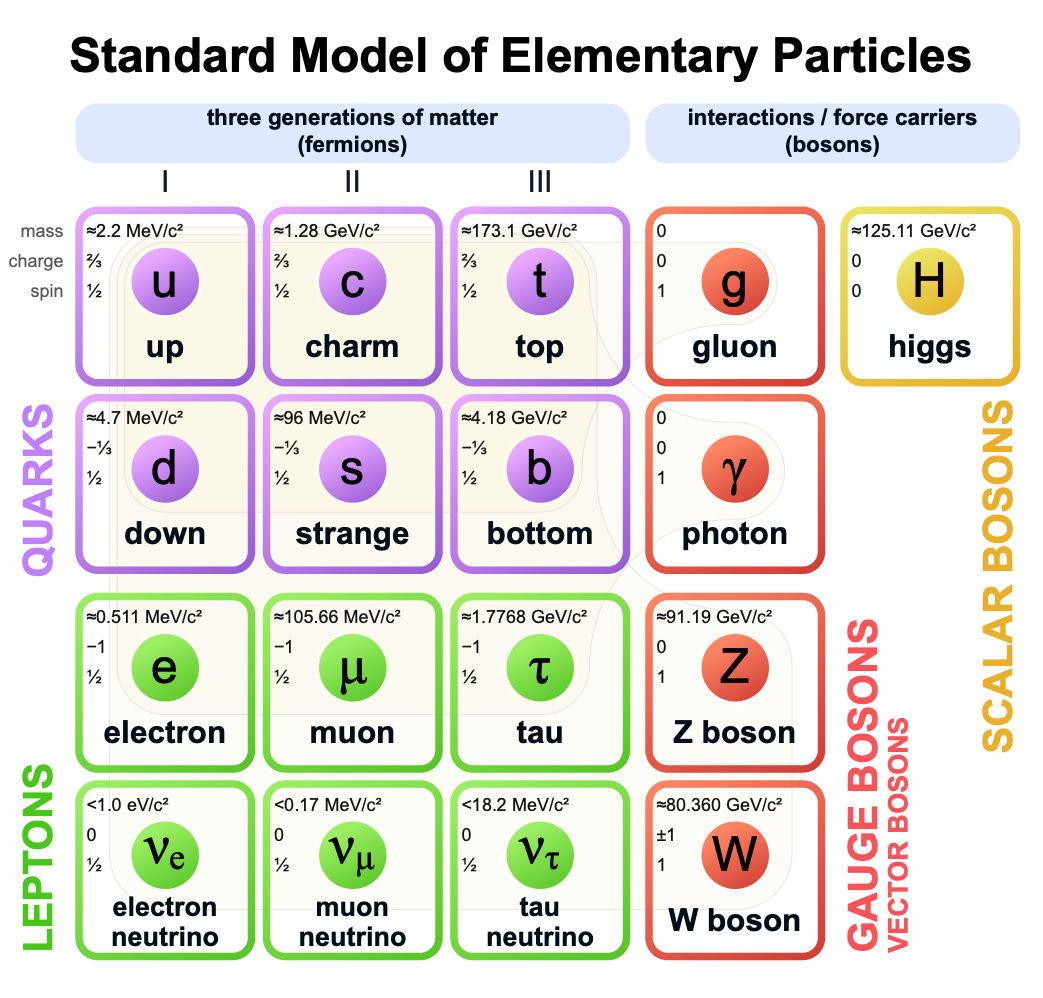
\includegraphics[width=8cm]{figures/ch-1-introduction/Standard_Model_of_Elementary_Particles.png}
    \caption{Table of Standard Model particles showing the grouping of the fermions into three generations of matter and the bosons, responsible for carrying the three fundamental forces in the Standard Model. The masses, charges, and spins of the particles are shown. The antimatter counterparts of the fermions are not shown. The possible interactions between the fermions and gauge bosons are highlighted.}
    \label{fig:intro-standard-model}
\end{figure}


Fermions consist of quarks and leptons, and are grouped into three generations. For example, the electron belongs to the first generation of leptons. The second and third generation counterparts of the electron are the muon and the tau lepton, and are over 200 and 30,000 times heavier than the electron respectively. Bosons are force carriers; the interaction of fermions with bosons corresponds to fundamental forces. The Standard Model describes the electromagnetic force, the strong nuclear force, and the weak nuclear force.


\section{The Standard Model as a gauge theory}
\label{section:SM-as-gauge-theory}

\subsection{Gauge invariance}
Gauge theories of elementary particle interactions originate from a freedom of choice in the mathematical description of particle fields which has no effect on the particles' physical states \cite{Tully+2012}. The existence and form of the particles' interactions, can be deduced from the existence of physically indeterminate, gaugable quantities.

An example of this gauge invariance is classical physics is the electromagnetic interaction, where the fundamental field is the four-vector potential $A^\mu$ \cite{Tully+2012}. The physical electromagnetic fields and Maxwell's equations arise from the elements of the tensor $F_{\mu\nu}(x) = \partial_\mu A_\nu (x) - \partial_\nu A_\mu (x)$. Any two choices of $A^\mu$ that are related by a transformation of the form

\begin{equation}
    A_\mu \rightarrow A_\mu + \partial_\mu \alpha
    \label{eqn:gauge_symmetry}
\end{equation} for any real, differentiable function $\alpha(x)$, describe the same physical configuration, and has no effect on Maxwell's equations. This ``redundancy'' in the choice of gauge in Eqn. \ref{eqn:gauge_symmetry} is called a gauge symmetry.

One important consequence of gauge symmetry comes from the application of Noether's theorem, which states that for every global transformation under which the Lagrangian density is invariant, there exists a conserved quantity. If $\mathcal{L}(\Psi(x), \partial_\mu \Psi(x))$ is invariant under the transformation of the wave function $\Psi(x) \rightarrow \Psi'(x)$, where $\Psi'(x) = \Psi(x) + \delta \Psi(x)$, then there exists a conserved current 
\begin{equation}
    \partial_\mu \left( \frac{\partial\mathcal{L}(x)}{\partial(\partial_\mu \Psi(x))} \delta \Psi(x)  \right) = 0
\end{equation}
In classical mechanics, the conservation of linear momentum, angular momentum, and energy follows from translational invariance, rotational variance, and invariance under translations in time \cite{Tully+2012}. Likewise, charge conservation can be shown to arise from the invariance of the Dirac Lagrangian density $\mathcal{L}_{\text{Dirac}} = \bar{\Psi} (i\gamma^\mu \partial_\mu -m)\Psi$ under the particle wavefunction's phase transformation, $\Psi'(x) = \exp(ie\chi) \Psi(x)$. Thus Noether's theorem establishes a correspondence between a gauge symmetry and a conserved internal property (e.g. charge or momentum).

\subsection{Local gauge symmetries}
Interactions between particles arise if we modify the wave function with a phase transformation $\Psi'(x) = \exp(i e \chi) \Psi(x)$, and allow the phase $\chi$ to be a function of spacetime \cite{Tully+2012}. A wave function of the form
\begin{equation}
    \Psi'(x) = \exp(i e \chi(x)) \Psi(x)
\end{equation}
can be verified to \textit{not} be a solution to the Dirac equation for free particles: $(i \gamma^\mu \partial_\mu - m) \Psi(x) = 0$. This necessitates a modified Dirac equation, where the derivative takes into account that the vector field $V(x)$ needs to be compared at two displaced space-time points in a curvilinear coordinate system: 
\begin{equation}
    \mathcal{D}_\mu \equiv \lim_{\Delta x^\mu \rightarrow 0} \frac{V_{\parallel}(x + \Delta x) - V(x)}
{\Delta x^\mu}\end{equation}
We define a covariant derivative, 
\begin{equation}
    D_\mu = \partial_\mu + i e A_\mu
\label{eqn:modified_dirac}
\end{equation}
where $A_\mu(x)$ is a 4-vector potential. Thus the modified Dirac equation reads:
\begin{equation}
    \left( i \gamma^\mu \mathcal{D}_\mu - m  \right) \Psi(x) = 0
\end{equation}
The simultaneous gauge transformation $A'_\mu(x) = A_\mu(x) - \partial_\mu\chi(x)$ and wavefunction transformation $\Psi'(x) = \exp(ie\chi(x)) \Psi(x)$ leaves the covariant-derivative form of the Dirac equation (Eqn \ref{eqn:gauge_symmetry}) invariant.

The generalization of this result is as follows: if a theory is invariant for unitary transformations $U$ of the particle states according to 
\begin{equation}
    \Psi' = U\Psi
\label{eqn:generic_unitary_transformation}
\end{equation}
One must define a derivative of the form
\begin{equation}
    D^\mu = \partial^\mu + ig B^\mu
\end{equation}
to keep the theory invariant under Eqn. \ref{eqn:generic_unitary_transformation}. The four-potential $B^\mu$ represents the interacting four-potential which must be added to keep the theory invariant.

In the case of the Standard Model, the theory is built around the gauge transformations $G = SU(3) \times SU(2) \times U(1)$. $SU(3)$ is associated to the strong force (subscripted $C$); $SU(2)$ is associated to the weak force (subscripted $L$); and $U(1)$ is hypercharge (subscripted Y). The gauge-covariant derivative  is 
\begin{equation}
    \mathcal{D}_\mu = \partial_\mu - ig' B_\mu \frac{Y}{2} - ig W_{\mu}^{\alpha} \frac{\tau_a}{2} - ig_s G_\mu^{k} \frac{\lambda_k}{2}
\end{equation}
\begin{itemize}
    \item In the $U(1)_Y$ term, $B_\mu$ is the weak hypercharge field.
    \item In the $SU(2)_L$ term, $W_\mu(x) = (W_\mu^1(x), W_\mu^2(x), W_\mu^3(x))$ are a triplet of four-potentials. $\tau/2$ are the Pauli matrices, generators of the $SU(2)$ transformation.
    \item In the $SU(3)_C$ term, the gluon (color) field is $G_\mu$. $\lambda_k$ are the Gell-Man matrices, generators of the $SU(3)$ transformation.
\end{itemize}   
The invariance of the Standard Model under $SU(3)_C \times SU(2)_L \times U(1)_Y$ requires massless fermions and massless force carriers.  

\section{The Higgs Mechanism}
\label{section:Higgs-mechanism}
To introduce mass into the theory, i.e. to change the propagation of the gauge particles and all the fermions, the physical vacuum cannot have all the symmetries of the Standard Model Lagrangian \cite{Tully+2012}. The symmetries of the physical vacuum must be spontaneously broken, without affecting gauge invariance in the Lagrangian. The Higgs mechanism proposes the existence of a scalar field, or fields, with nonzero vacuum expectation values, which reduce the gauge symmetries of the physical vacuum from $SU(3)_C \times SU(2)_L \times U(1)_Y$ down to $SU(3)_C \times U(1)_{EM}$.

The Higgs field interacts with the gauge bosons and fermions throughout space, impeding their free propagation. The resulting broken symmetry correctly predicts the mass ratio of the neutral (Z) and charged (W) massive electroweak bosons, and predicts that at least one physical degree of freedom in the Higgs field is a particle degree of freedom, called the Higgs boson. The location of the minimum of the Higgs potential can be constrained from previously measured Standard Model parameters, but the shape of the mass distribution of the Higgs boson must be experimentally measured.

The minimal choice of Higgs field comes from the breaking of $SU(2)_L \times U(1)_Y$ down to $U(1)_{EM}$. The smallest $SU(2)$ multiplet is the doublet. The existence of three massive electroweak bosons leads the Higgs sector to have at least three degrees of freedom. The minimal single-doublet complex scalar Higgs field is
\begin{equation}
    \Phi(x) = \begin{pmatrix} \phi^+(x) \\ \phi^0(x) \end{pmatrix} 
    = \frac{1}{\sqrt{2}} \begin{pmatrix} \phi_1^+(x) + i\phi_2^+(x) \\ \phi_1^0(x) + i\phi_2^0 (x) \end{pmatrix}
\end{equation}
where $\phi_1^+$, $\phi_2^+$, $\phi_1^0$, and $\phi_2^0$ are real (four degrees of freedom). By convention, the nonzero vacuum expectation value is assigned to $\phi_1^0$.

The minimal self-interacting Higgs potential that is invariant under $SU(2)_L \times U(1)_Y$ is given by
\begin{equation}
    V(\Phi^\dagger \Phi) = -\mu^2 \Phi^\dagger \Phi + \lambda (\Phi^\dagger \Phi)^2, \,\,\, \mu^2 > 0, \, \lambda > 0
\end{equation}
where $\lambda$ is the coupling strength of the four-point Higgs interaction. 
The potential energy is minimized at 
\begin{equation}
    \Phi_{\text{min}} = \frac{1}{\sqrt{2}} \begin{pmatrix} 0 \\ v \end{pmatrix}, \,\,\,\text{where} \, v = \sqrt{\mu^2 / \lambda}
\end{equation}
Choosing a fixed orientation of $\langle \Phi \rangle$ out of a continuous set of possible ground states spontaneously breaks the symmetry of the physical vacuum, as illustrated in Fig \ref{fig:higgs-potential}.

\begin{figure}[ht]
    \centering
    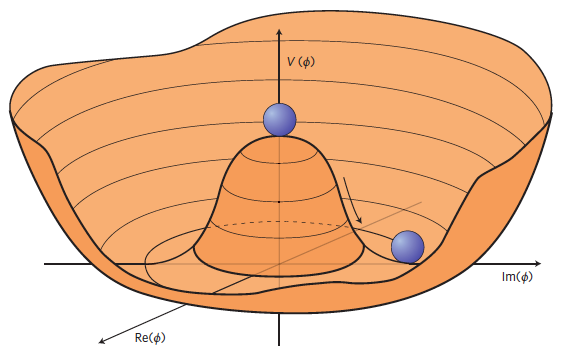
\includegraphics[width=8cm]{figures/ch-1-introduction/higgs-potential.png}
    \caption[An illustration of the Higgs potential.]{An illustration of the Higgs potential \cite{Ellis:2013jnq}. Choosing any of the points at the bottom of the potential breaks spontaneously the rotational $U(1)$ symmetry.}
    \label{fig:higgs-potential}
\end{figure}

The excitations of the Higgs field with respect to the minimum $\Phi_{\text{min}}$ are parameterized by 
\begin{equation}
    \Phi(x) = \exp(i \boldsymbol{\xi}(x) \cdot \boldsymbol{\tau}) \frac{1}{\sqrt{2}} \begin{pmatrix} 0 \\ v + H(x) \end{pmatrix}
\end{equation}
Three degrees of freedom are coupled directly to the electroweak gauge bosons; this is often referred to as the gauge bosons ``eating'' the Goldstone bosons to form the longitudinal polarizations of the massive spin-1 boson states. The $H(x)$ excitation is in the radial direction and corresponds to the free particle state of the Higgs boson. 

\section{Two-Higgs Doublet Models}
\label{section:theory-2HDM}

One of the simplest possible extensions to the Standard Model is adding a doublet to the minimal Higgs sector of the Standard Model, which is a $SU(2)_L$ doublet $H$ with hypercharge $Y = +\frac{1}{2}$, denoted here as $H \sim 2_{+1/2}$. These extensions are found in several theories such as supersymmetry. A general 2HDM can be extended with a light scalar (2HDM+S) to obtain a rich set of exotic Higgs decays \cite{2HDM-PhysRevD.90.075004}. 

The charges of the Higgs fields are chosen to be $H_1 \sim 2_{-1/2}$ and $H_2 \sim 2_{+1/2}$, which acquire vacuum expectation values $v_{1,2}$ which are assumed to be real and aligned \cite{2HDM-PhysRevD.90.075004}. Expanding about the minima yields two complex and four real degrees of freedom:
\begin{align}
    H_1 &= \frac{1}{\sqrt{2}} \begin{pmatrix} v_1 + H^{0}_{1, R} + iH^0_{1, I} \\  
                                              H^-_{1,R} + i H^-_{1, I}   \end{pmatrix} \\
    H_2 &= \frac{1}{\sqrt{2}} \begin{pmatrix} H^+_{2, R} + iH^+_{2, I} \\  
                                              v_2 + H^0_{2,R} + i H^0_{2, I}   \end{pmatrix} 
\end{align}

The charged scalar and pseudoscalar mass matrices are diagonalized by a rotation angle $\beta$, defined as $\tan\beta = v_2/v_1$. One charged (complex) field and one neutral pseudoscalar combination of $H^0_{1, 2, I}$ are eaten by the SM gauge bosons after electroweak symmetry breaking \cite{2HDM-PhysRevD.90.075004}. The other complex field yields two charged mass eigenstates $H^\pm$, which are assumed to be heavy. The remaining three degrees of freedom yield one neutral pseudoscalar mass eigenstate 
\begin{equation}
    A = H^0_{1, I}\sin\beta - H^0_{2, I} \cos\beta
\end{equation}
and two neutral scalar mass eigenstates (where $-\pi/2 \leq \alpha \leq pi/2$)
\begin{equation}
    \begin{pmatrix} h \\ H^0 \end{pmatrix} = \begin{pmatrix} -\sin\alpha & \cos\alpha \\
                                                              \cos\alpha & \sin\alpha \end{pmatrix}
                                             \begin{pmatrix} H^0_{1, R} \\ H^0_{2, R}  \end{pmatrix}
\end{equation}
We assume that the 2HDM is near or in the decoupling limit: $\alpha \rightarrow \pi/2 - \beta$, where the lightest state in the 2HDM is $h$, which we identify as the 125 GeV Higgs particle \cite{2HDM-PhysRevD.90.075004}. In this limit, the fermion couplings of $h$ become identical to the Standard Model Higgs, while the gauge boson couplings are very close to Standard Model-like for $\tan\beta \gtrsim 5$. All of the properties of $h$ are determined by just two parameters: $\tan\beta$ and $\alpha$, and the fermion couplings to the two Higgs doublets. 

2HDM can be extended by a scalar singlet (2HDM+S) \cite{2HDM-PhysRevD.90.075004}:
\begin{equation}
    S = \frac{1}{\sqrt{2}} (S_R + iS_I)
\end{equation}
If this singlet only couples to the Higgs doublets $H_{1,2}$ and has no direct Yukawa couplings, all of its couplings to SM fermions result from mixing with $H_{1,2}$. Under these simple assumptions, exotic Higgs decays $h\rightarrow ss \rightarrow X\bar{X}Y\bar{Y}$ or $h\rightarrow aa \rightarrow X\bar{X}Y\bar{Y}$, and $h \rightarrow aZ \rightarrow X\bar{X}Y\bar{Y}$ are permitted, where $s(a)$ is a (pseudo)scalar mass eigenstate mostly composed of $S_R (S_I)$, and $X, Y$ are Standard Model fermions or gauge bosons. There are two pseudoscalars in the 2HDM+S, and the mostly singlet-like pseudoscalar can be chosen to be the one lighter than the SM-like Higgs. For $m_a < m_h - m_Z \sim 35$ GeV, the exotic Higgs decay $h \rightarrow Za$ is possible, and for $m_a < m_h/2 \approx 63$ GeV, the exotic Higgs decay $h \rightarrow aa$ is possible. 

\begin{figure}[ht]
    \centering
    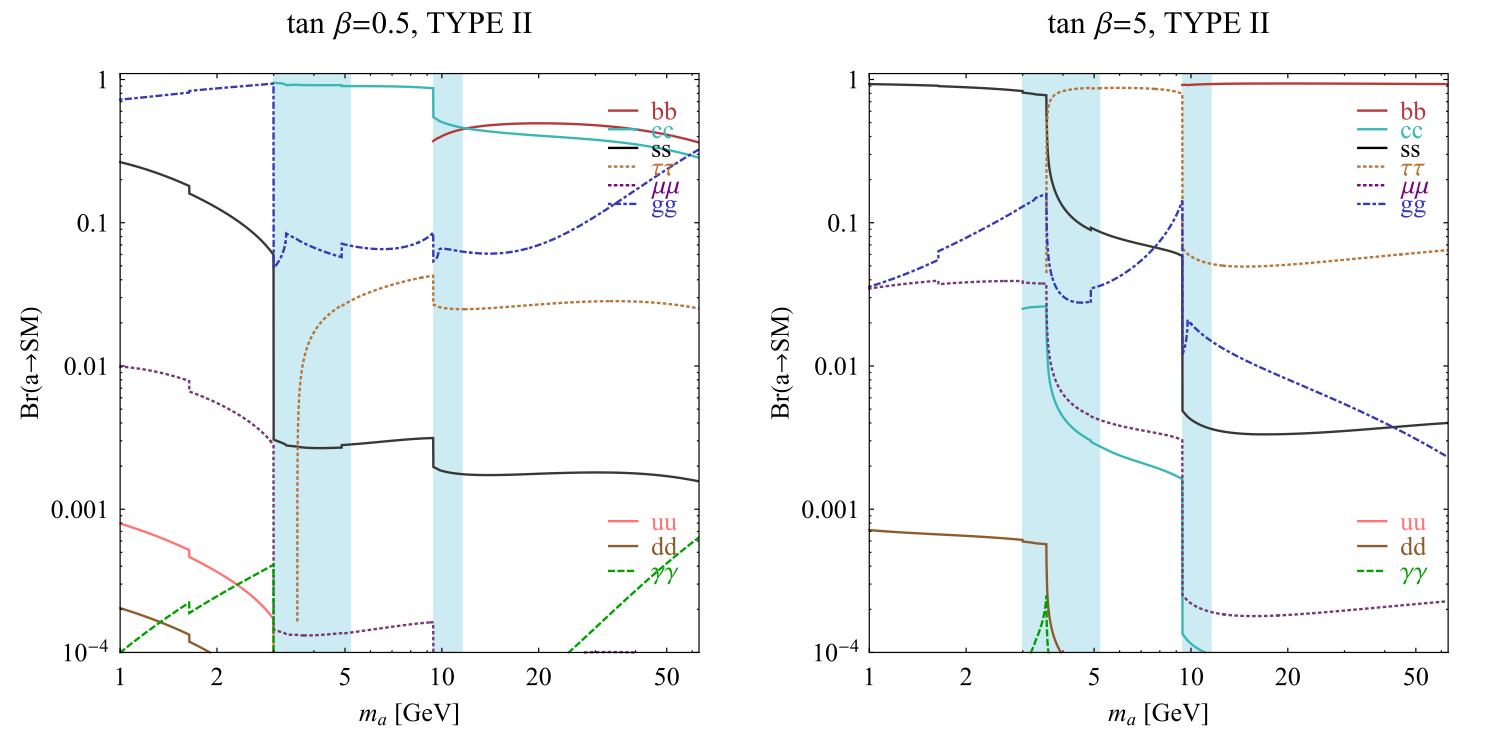
\includegraphics[width=15cm]{figures/ch-1-introduction/curtin-2014-figure-7-BRs-of-singlelike-pseudoscalar-type-II.png}
    \caption[Branching ratios of a singlet-like pseudoscalar in Type II 2HDM+S for $\tan\beta = 0.5$ (left) and $\tan\beta = 5$ (right).]{Branching ratios of a singlet-like pseudoscalar in Type II 2HDM+S for $tan\beta = 0.5$ (\textit{left}) and $\tan\beta = 5$ (\textit{right}) from \cite{2HDM-PhysRevD.90.075004}, showing the dependence of the branching ratios on $\tan\beta$, as well as the prominence of the branching ratios to $bb$ and $\tau\tau$, the channels searched for in the analysis presented here.}
    \label{fig:curtin-2014-fig-4-typeI-BRs}
\end{figure}


In 2HDM, and by extension 2HDM+S, there are four types of fermion couplings commonly discussed in the literature that forbid flavor-changing neutral currents at tree level \cite{2HDM-PhysRevD.90.075004}. These are referred to as Type I (all fermions couple to $H_2$), Type II (MSSM-like, $d_R$ and $e_R$ couple to $H_1$, $u_R$ to $H_2$), Type III (lepton-specific, leptons and quarks couple to $H_1$ and $H_2$ respectively) and Type IV (flipped, with $u_R$, $e_R$ coupling to $H_2$ and $d_R$ to $H_1$). The exact branching ratios of the pseudoscalars to Standard Model particles vary depending on the 2HDM+S model and the value of $\tan\beta$ (e.g. Fig. \ref{fig:curtin-2014-fig-4-typeI-BRs}).

\section{Two Real Singlet Model}
\label{section:theory-TRSM}
The two real singlet model (TRSM) adds two real singlet degrees of freedom to the Standard Model. These are written as two real singlet fields $S$ and $X$. Depending on the vacuum expectation values acquired by the scalars, different phases of the model can be realized \cite{Robens:2019kga}. To reduce the number of free parameters, two discrete $\mathbb{Z}_2$ symmetries are introduced. The fields are decomposed as

\begin{equation}
    \Phi = \begin{pmatrix} 0 \\ \frac{\phi_h + v}{\sqrt{2}} \end{pmatrix}, 
    \,
    S = \frac{\phi_S + v_S}{\sqrt{2}} ,
    \,
    X = \frac{\phi_X + v_X}{\sqrt{2}}
\end{equation}
To achieve electroweak-breaking symmetry, $v  = v_{SM} \sim 246$ 246 GeV is necessary. If the vacuum expectation values $v_S, v_X \neq 0$ the $\mathbb{Z}_2$ are spontaneously broken, and the fields $\phi_{h,S,X}$ mix into three physical scalar states. This is called the broken phase and leads to the most interesting collider phenomenology.

The mass eigenstates $h_{1,2,3}$ are related to the fields $\phi_{h,S,X}$ through a $3\times 3$ orthogonal mixing matrix denoted $R$. The mass eigenstates are assumed to be ordered $M_1 \leq M_2 \leq M_3$. $R$ is parameterized by the three mixing angles $\theta_{hS}$, $\theta_{hX}$, $\theta_{SX}$. The nine parameters of the scalar potential can be expressed in terms of the three physical Higgs masses, the three mixing angles, and the three vacuum expectation values. 

After fixing one of the Higgs masses to the mass of the observed Higgs boson, and fixing the Higgs doublet vacuum expectation value to its Standard Model value, there are seven remaining free parameters of the TRSM \cite{Robens:2019kga}.

In one benchmark scenario of TRSM \cite{Robens:2019kga}, the heaviest scalar state $h_3$ is identified with the 125 GeV Higgs, $h_{125}$, and it can decay asymmetrically $h_{125} \rightarrow h_1 h_2$, which we also denote $h \rightarrow a_1 a_2$ to highlight the similarity with the symmetric decay $h \rightarrow aa$ typically interpreted in 2HDM+S as discussed. The parameter values in TRSM are chosen such that the coupling of $h_3$ to Standard Model particles are nearly identical to the Standard Model predictions. 

\begin{figure}[ht]
    \centering
    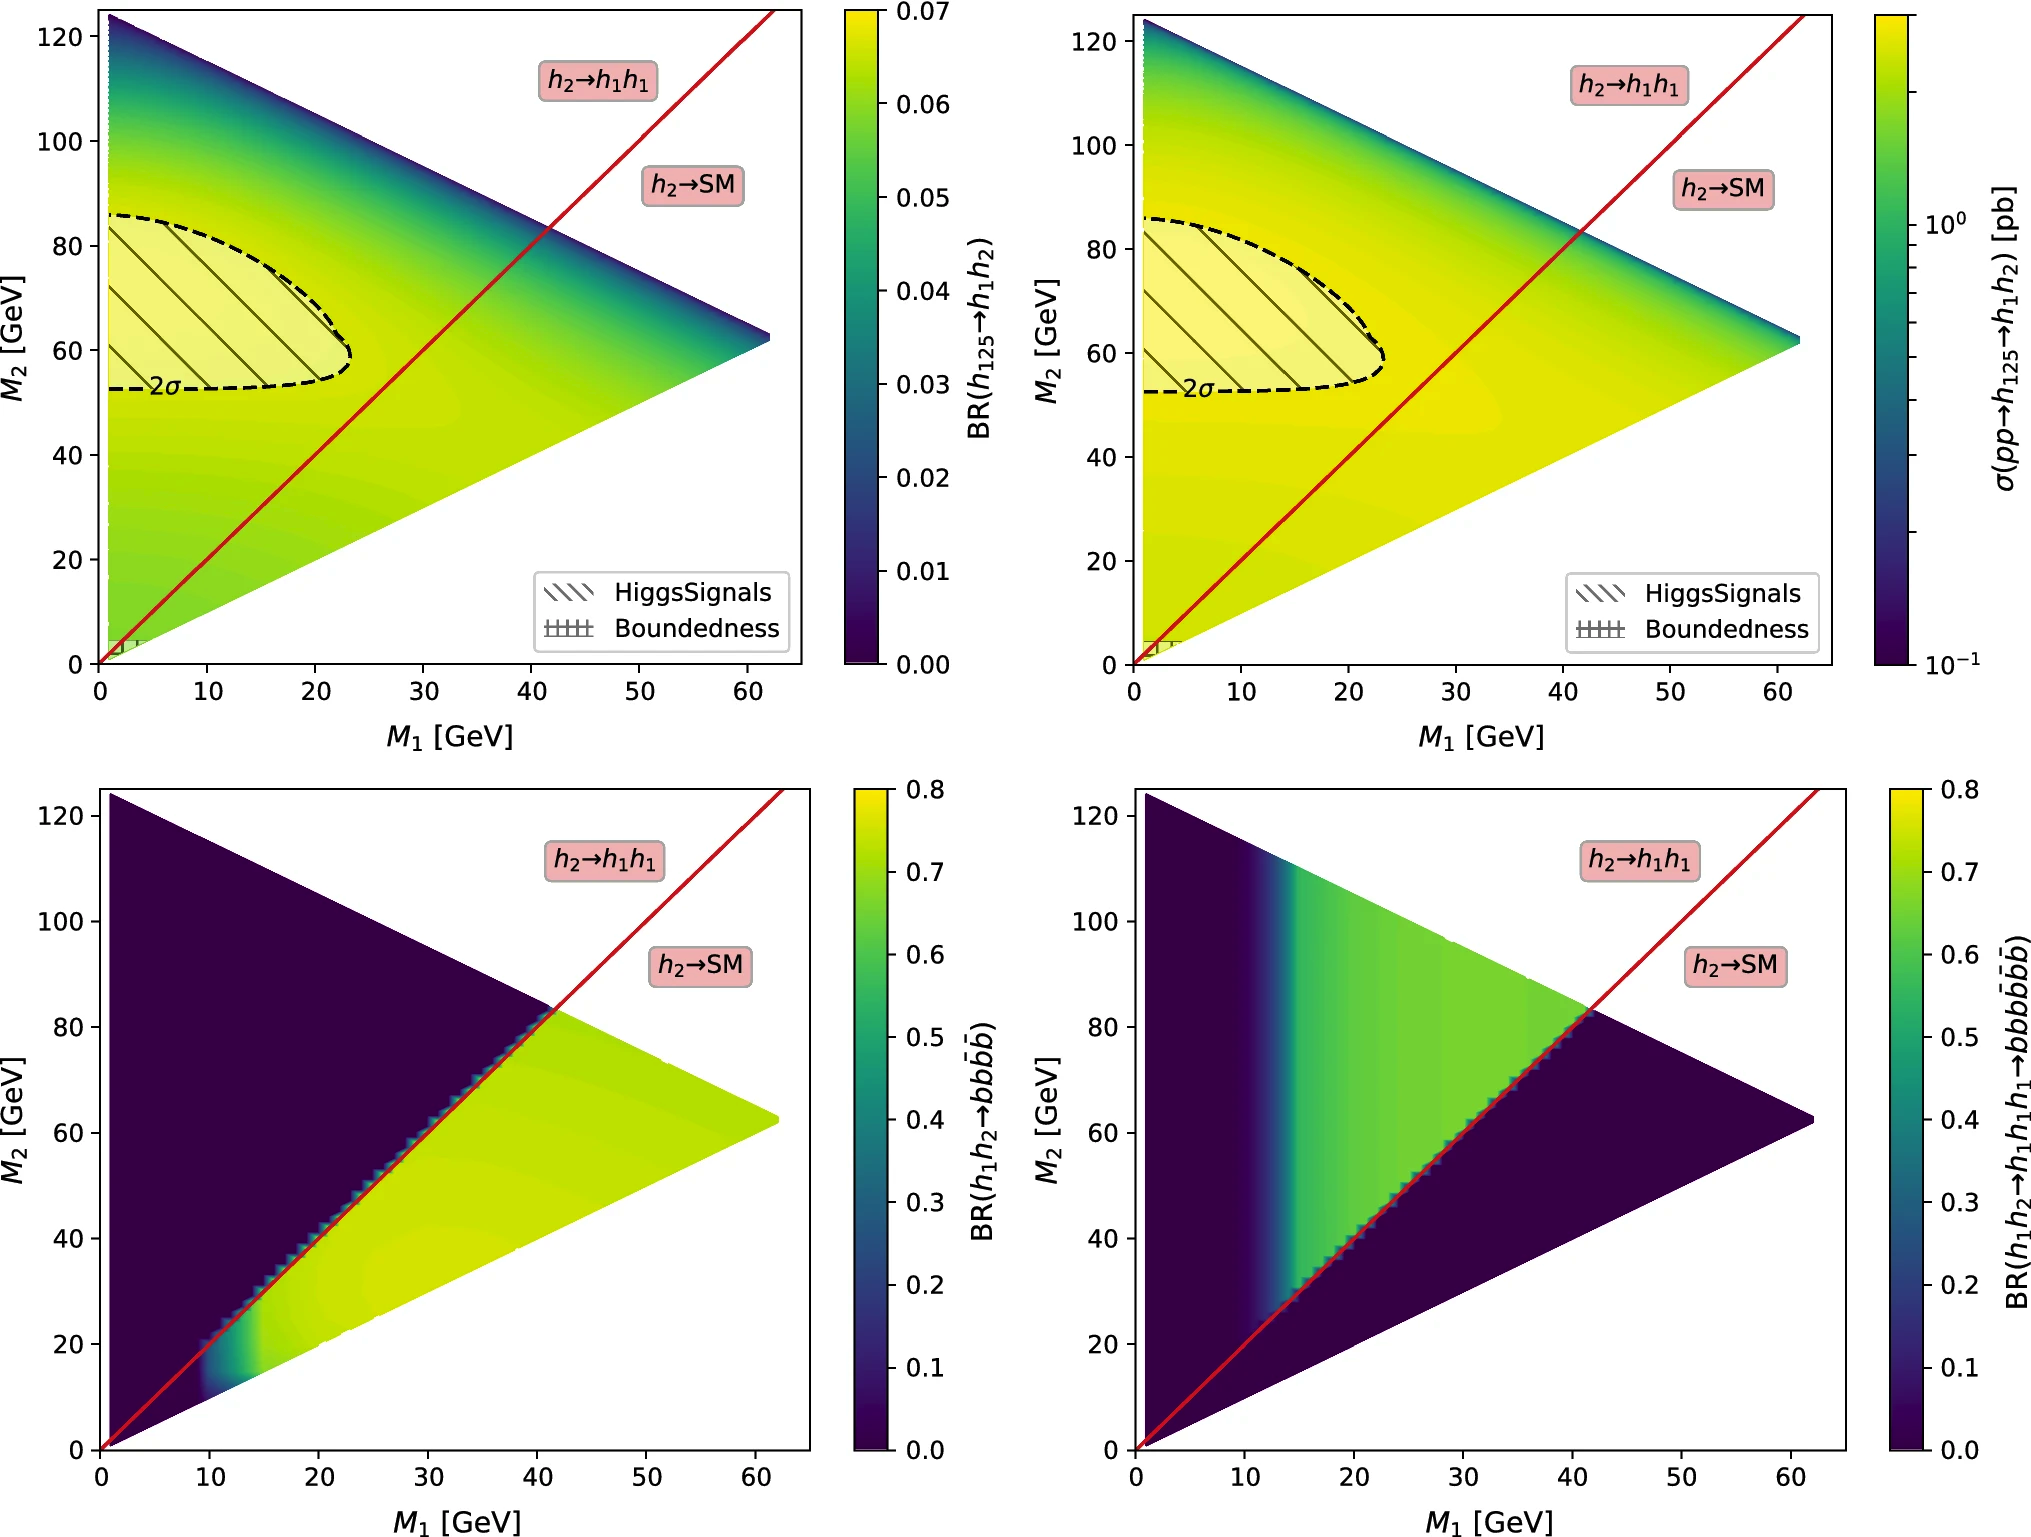
\includegraphics[width=15cm]{figures/ch-1-introduction/Robens-TRSM-Figure-6-BP-1.png}
    \caption[Benchmark plane BP1 for benchmark scenario 1, for the decay signature $h_{125} \rightarrow h_1 h_2$ with $h_{125} \equiv h_3$, defined in the $(M_1, M_2)$ plane.]{Benchmark plane BP1 for benchmark scenario 1 from \cite{Robens:2019kga}, for the decay signature $h_{125} \rightarrow h_1 h_2$ with $h_{125} \equiv h_3$, defined in the $(M_1, M_2)$ plane. The color code shows BR$(h_3 \rightarrow h_1 h_2)$ (\textit{top left}) and the 13 TeV LHC signal rate for $pp \rightarrow h_3 \rightarrow h_1 h_2$ (\textit{top right}). The red line separates the region $M_2 > 2 M_1$, where BR($h_2 \rightarrow h_1 h_1$) $\sim 100\%$, from the region $M_2 < 2 M_1$, where BR($h_2 \rightarrow F_{SM}$) $\sim 100\%$. The \textit{bottom left} and \textit{right} show the branching ratio of the $h_1 h_2$ into (respectively) $b\bar{b}b\bar{b}$, and through a $h_2 \rightarrow h_1 h_1$ cascade to $b\bar{b}b\bar{b}b\bar{b}$. The hatched region indicates where the decay rate slightly exceeds the $2\sigma$ upper limit inferred from the LHC Higgs rate measurements, though the region depends on the parameter choices and experimental searches should cover the whole mass range.}
    \label{fig:trsm_bp1}
\end{figure}

In benchmark scenario 1 (benchmark plane 1, or BP1) (Fig. \ref{fig:trsm_bp1}) \cite{Robens:2019kga}, the maximal branching ratios for $h_3 \rightarrow h_1 h_2$ reach up to $7-8\%$ which translates into a signal rate of around 3 pb. These maximal branching ratios are reached in the intermediate mass state for $h_2$, $M_2 \sim 60 - 80$ GeV. For $M_2 < 40$ GeV, although phase space opens up significantly for light decay products, the branching ratio becomes smaller. 

If the decay channel $h_2 \rightarrow h_1 h_1$ is kinematically open (i.e. $M_2 > 2M_1$), it is the dominant decay mode leading to a significant rate for the $h_1 h_1 h_1$ final state, in a ``cascade" decay. In BP1, $BR(h_2 \rightarrow h_1h_1$) $\simeq 100\%$ above the red line in Fig. \ref{fig:trsm_bp1}. If, in addition, $M_1 \gtrsim 10$ GeV, the $h_1$ decays dominantly to $b\bar{b}$ leading to a sizable rate for the $b\bar{b}b\bar{b}b\bar{b}$ final state as shown in Fig. \ref{fig:trsm_bp1} (\textit{bottom right}).

If the $h_2 \rightarrow h_1 h_1$ decay is kinematically closed (i.e. $M_2 < 2M_1$), both scalars decay directly to Standard Model particles, with branching ratios identical to a Standard Model-like Higgs boson, i.e. with the $b\bar{b}b\bar{b}$ final state dominating, as shown in Fig. \ref{fig:trsm_bp1} (\textit{bottom left}), while at smaller masses, combinations with $\tau$ leptons and eventually final states with charm quarks and muons become relevant \cite{Robens:2019kga}.


\chapter{The Large Hadron Collider and the CMS Experiment}
This chapter introduces the key aspects of the CERN Large Hadron Collider (LHC) and the Compact Muon Solenoid (CMS) experiment where the work for this thesis was conducted. Section \ref{section:LHC} describes the history of accelerator developments at CERN that led to the construction of the LHC, the current LHC configuration, and the largest experiments located at the LHC. The concepts of beam luminosity and pileup, which are critical for understanding and measuring high-energy particle collisions, are described in Section \ref{section:luminosity_and_pileup} and discussed in the context of the High-Luminosity LHC (HL-LHC) upgrade in Section \ref{section:HL-LHC}. Lastly, Section \ref{section:cms-detector} describes the design and function of CMS and its subdetectors, and terminates in a description of data processing at CMS, beginning from online event filtering in the Level-1 Trigger, to processing in the High-Level Trigger, to offline particle reconstruction, and finally long-term storage and processing of measured events.

\section{The Large Hadron Collider}
\label{section:LHC}
CERN, the European Organization for Nuclear Research, is an international organization based in Meyrin, Switzerland which operates the world's largest particle physics laboratory, and is the site of the Large Hadron Collider (LHC) \cite{history_of_CERN}. The very first accelerator built at CERN was the 600 MeV Synchrocyclotron (SC), which initially provided beams for CERN's first experiments. The newer and more powerful Proton Synchrotron (PS), which could accelerate particles to an energy of 28\GeV, began operations in 1959 and is still in use today. The first hadron collider at CERN was the Intersecting Storage Rings (ISR), which consisted of two interlaced rings each with a diameter of 200. The ISR collided protons at a center-of-mass energy of 62\GeV and began measuring collisions in 1971. In 1968 CERN began to accelerate heavy ions in the Super Proton Synchrotron (SPS), which is 7 kilometers in circumference and was the first of CERN's giant underground rings to be built. The SPS became the forefront of CERN's particle physics program in 1976, and in 1981 was converted into a proton-antiproton collider. The final and largest underground ring constructed at CERN was the Large Electron-Positron (LEP) collider, which was commissioned in July 1989 and hosted 5176 magnets and 128 accelerating cavities located around a 27-kilometer circumference. Over 11 years of research, four detectors, ALEPH, DELPHI, L3, and OPAL measured the collisions, with collision energies reaching up to 209\GeV in the year 2000. In November 2000, LEP was closed down to make way for the construction of the LHC in the same tunnel.

In its current configuration, the LHC accelerator complex at CERN is a succession of machines that accelerate particles in stages until they reach their final energy of 6.5 TeV per beam \cite{CERN-OPEN-2000-148} \cite{Linac4-design-report-2020}. In Linear accelerator 4 (Linac4), negative hydrogen ions (hydrogen atoms with an additional electron) are accelerated to 160 MeV, and stripped of their two electrons, leaving only protons, before entering the Proton Synchrotron Booster (PSB). These protons are accelerated to 2\GeV, then to 26\GeV in the Proton Synchrotron (PS), and 450\GeV in the Super Proton Synchrotron (SPS). The protons are transferred to the two beam pipes of the Large Hadron Collider (LHC). The LHC is a 27-kilometer ring of superconducting magnets, inside which one beam circulates clockwise and the other counterclockwise. Each LHC ring takes 4 minutes and 20 seconds to fill, and it takes about 20 minutes for the protons to reach their maximum energy. During normal operating conditions, beams circulate for many hours inside the LHC ring. 

The beams of particles in the LHC are made to collide at a center-of-mass energy of up to 14 TeV, at four positions at particle detector experiments located around the ring: ATLAS, CMS, ALICE, and LHCb. An aerial view of the four major experiments' locations is shown in Fig. \ref{fig:aerial-view-LHC-ring} \cite{OPEN-PHO-ACCEL-2017-005}. ATLAS and CMS are the two general-purpose detectors with broad physics programmes spanning Standard Model measurements and searches for signatures of new physics \cite{ATLAS-TDR-14} \cite{CERN-LHCC-2006-001}. The two experiments use different technical solutions and different magnet system designs. ALICE is a general-purpose detector dedicated to measuring LHC heavy-ion collisions, and is designed to address the physics of strongly interacting matter, and the properties of quark-gluon plasma \cite{ALICE-original-TDR}. The LHCb experiment specializes in investigating CP violation through measuring the differences in matter and antimatter, by using a series of subdetectors to detect mainly forward particles close to the beam direction \cite{LHCb-1998}. 

\begin{figure}[ht]
    \centering
    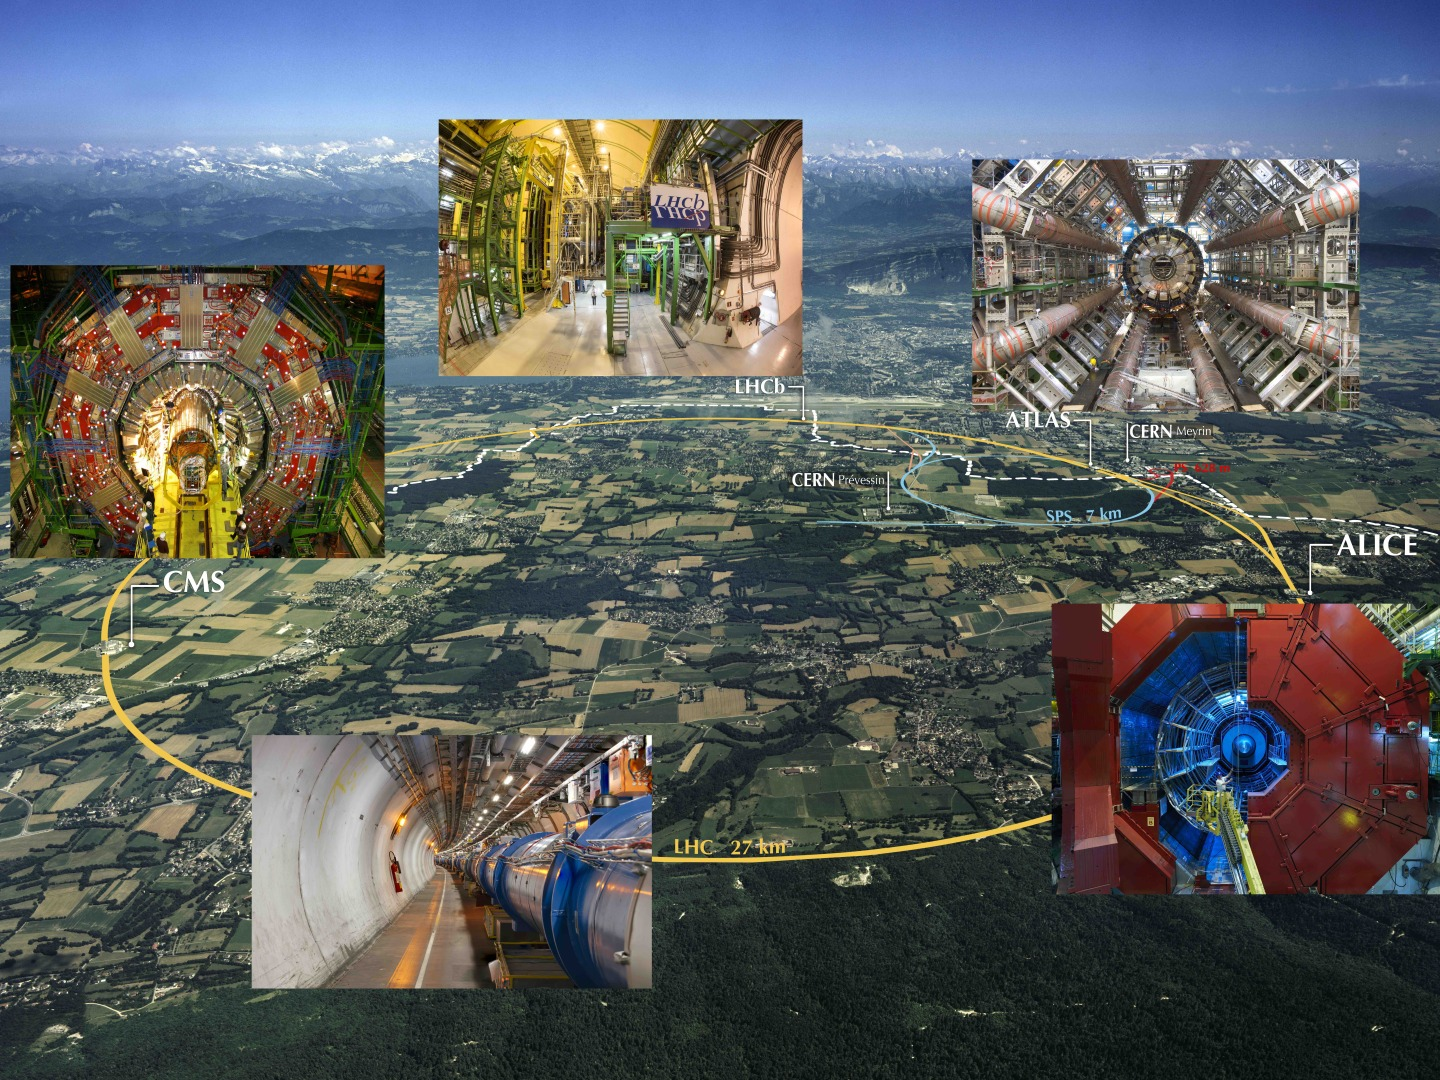
\includegraphics[width=11cm]{figures/ch-2-cern-cms/aerial-view-LHC-ring.jpeg}
    \caption[Aerial view of the Large Hadron Collider (LHC).]{Aerial view of the Large Hadron Collider (LHC) spanning the border of France and Switzerland, and the four major experiments located around the ring: CMS (Compact Muon Solenoid), LHCb (LHC beauty), ATLAS (A Toroidal LHC Apparatus), and ALICE (A Large Ion Collider Experiment) \cite{OPEN-PHO-ACCEL-2017-005}.}
    \label{fig:aerial-view-LHC-ring}
\end{figure}



\section{Luminosity and pileup}
\label{section:luminosity_and_pileup}
In order to search for rare decays, such as those that result from the creation and decay of a Higgs, W, or Z boson, a large number of parton interactions per second are required at the LHC. The number of events generated per second by the LHC collisions is given by
\begin{equation}
     N_{event} = \mathcal{L} \cdot \sigma_{event}
    \label{eqn:nEvents}
\end{equation} 
where $\sigma_{event}$ is the cross-section for the event under study, and $\mathcal{L}$ the instantaneous luminosity. The instantaneous luminosity is measured in units of cm$^{-2}$ s$^{-1}$, and depends only on the beam parameters, and can be written for a Gaussian beam distribution as:
\begin{equation}
    \mathcal{L} = \frac{N_b^2 n_b f_{rev} \gamma_r}{4\pi \epsilon_n \beta^*} F
\end{equation}
where the parameters are as defined, along with some example typical nominal values in Phase-1 of the LHC \cite{CERN-luminosity-accelerator-school-article} \cite{ipac2012-proceedings}:
% reference: material included in introduction to accelerator physics 2021 https://indico.cern.ch/event/1001431/contributions/

\begin{itemize}
    \item $N_b$ is the number of particles per bunch ($N_b \approx 1.15 \times 10^{11}$ protons per bunch)
    \item $n_b$ is the number of bunches per beam (maximum 2808),
    \item $f_{rev}$ is the revolution frequency ($\approx 11$ kHz),
    \item $\gamma_r$ is the relativistic gamma factor,
    \item $\epsilon_n$ is the normalized transverse beam emittance (area in a transverse plane occupied by the beam particles),
    \item $\beta^*$ is the beta function at the collision point ($\beta^* = 0.55$ m),
    \item and $F$ is the geometric luminosity reduction factor due to the crossing angle at the interaction points ($F \approx 0.84$ for Phase-1. Note that complete overlap would give $F = 1$).
\end{itemize}
Peak luminosity at interaction points 1 and 5 reach values of $\sim 1.0 \times 10^{34}$ cm$^{-2}$ s$^{-1}$, with peak luminosity per bunch crossing reaching $\sim 3.56 \times 10^{34}$ cm$^{-2}$ s$^{-1}$.

Per Eqn. \ref{eqn:nEvents}, the integrated luminosity over time is proportional to the number of events produced, and the size of LHC datasets is commonly presented in terms of integrated luminosity. Collider operation aims to optimize the integrated luminosity. Thus the exploration of rare events in the LHC collisions requires both high beam energies and high beam intensities.

The LHC's nominal beam luminosities are sufficiently large for multiple proton-proton collisions to occur in the same time window of 25 nanoseconds in which proton bunches collide \cite{CMS-JME-18-001}. These multiple collisions will lead to particle interactions overlapping in the detector. To measure a proton-proton collision, the single collision must be separated from overlapping collisions, which are called ``pileup'' collisions. A distribution of pileup in the data-taking years 2016-2018 is shown in Fig. \ref{fig:pileup-run-2}. The pileup is defined as the average number of $pp$ collisions per bunch crossing.

CMS reports an inelastic $pp$ cross section of $\sigma_{\text{inel}} = 68.6$ millibarns at a center-of-mass energy of $\sqrt{s} = 13$ TeV \cite{CERN-EP-2018-004-pileup}, which can be used to estimate pileup as follows:
\begin{equation}
    \text{Pileup} = \frac{\mathcal{L} \times \sigma_{\text{inel}}}{ n_b \cdot f}
\end{equation}
With the example values above, pileup can be estimated to be $\sim 22$.

Thus, higher luminosities create more intense pileup conditions, posing a greater challenge to detector performance and particle reconstruction and identification.

\begin{figure}[ht]
    \centering
    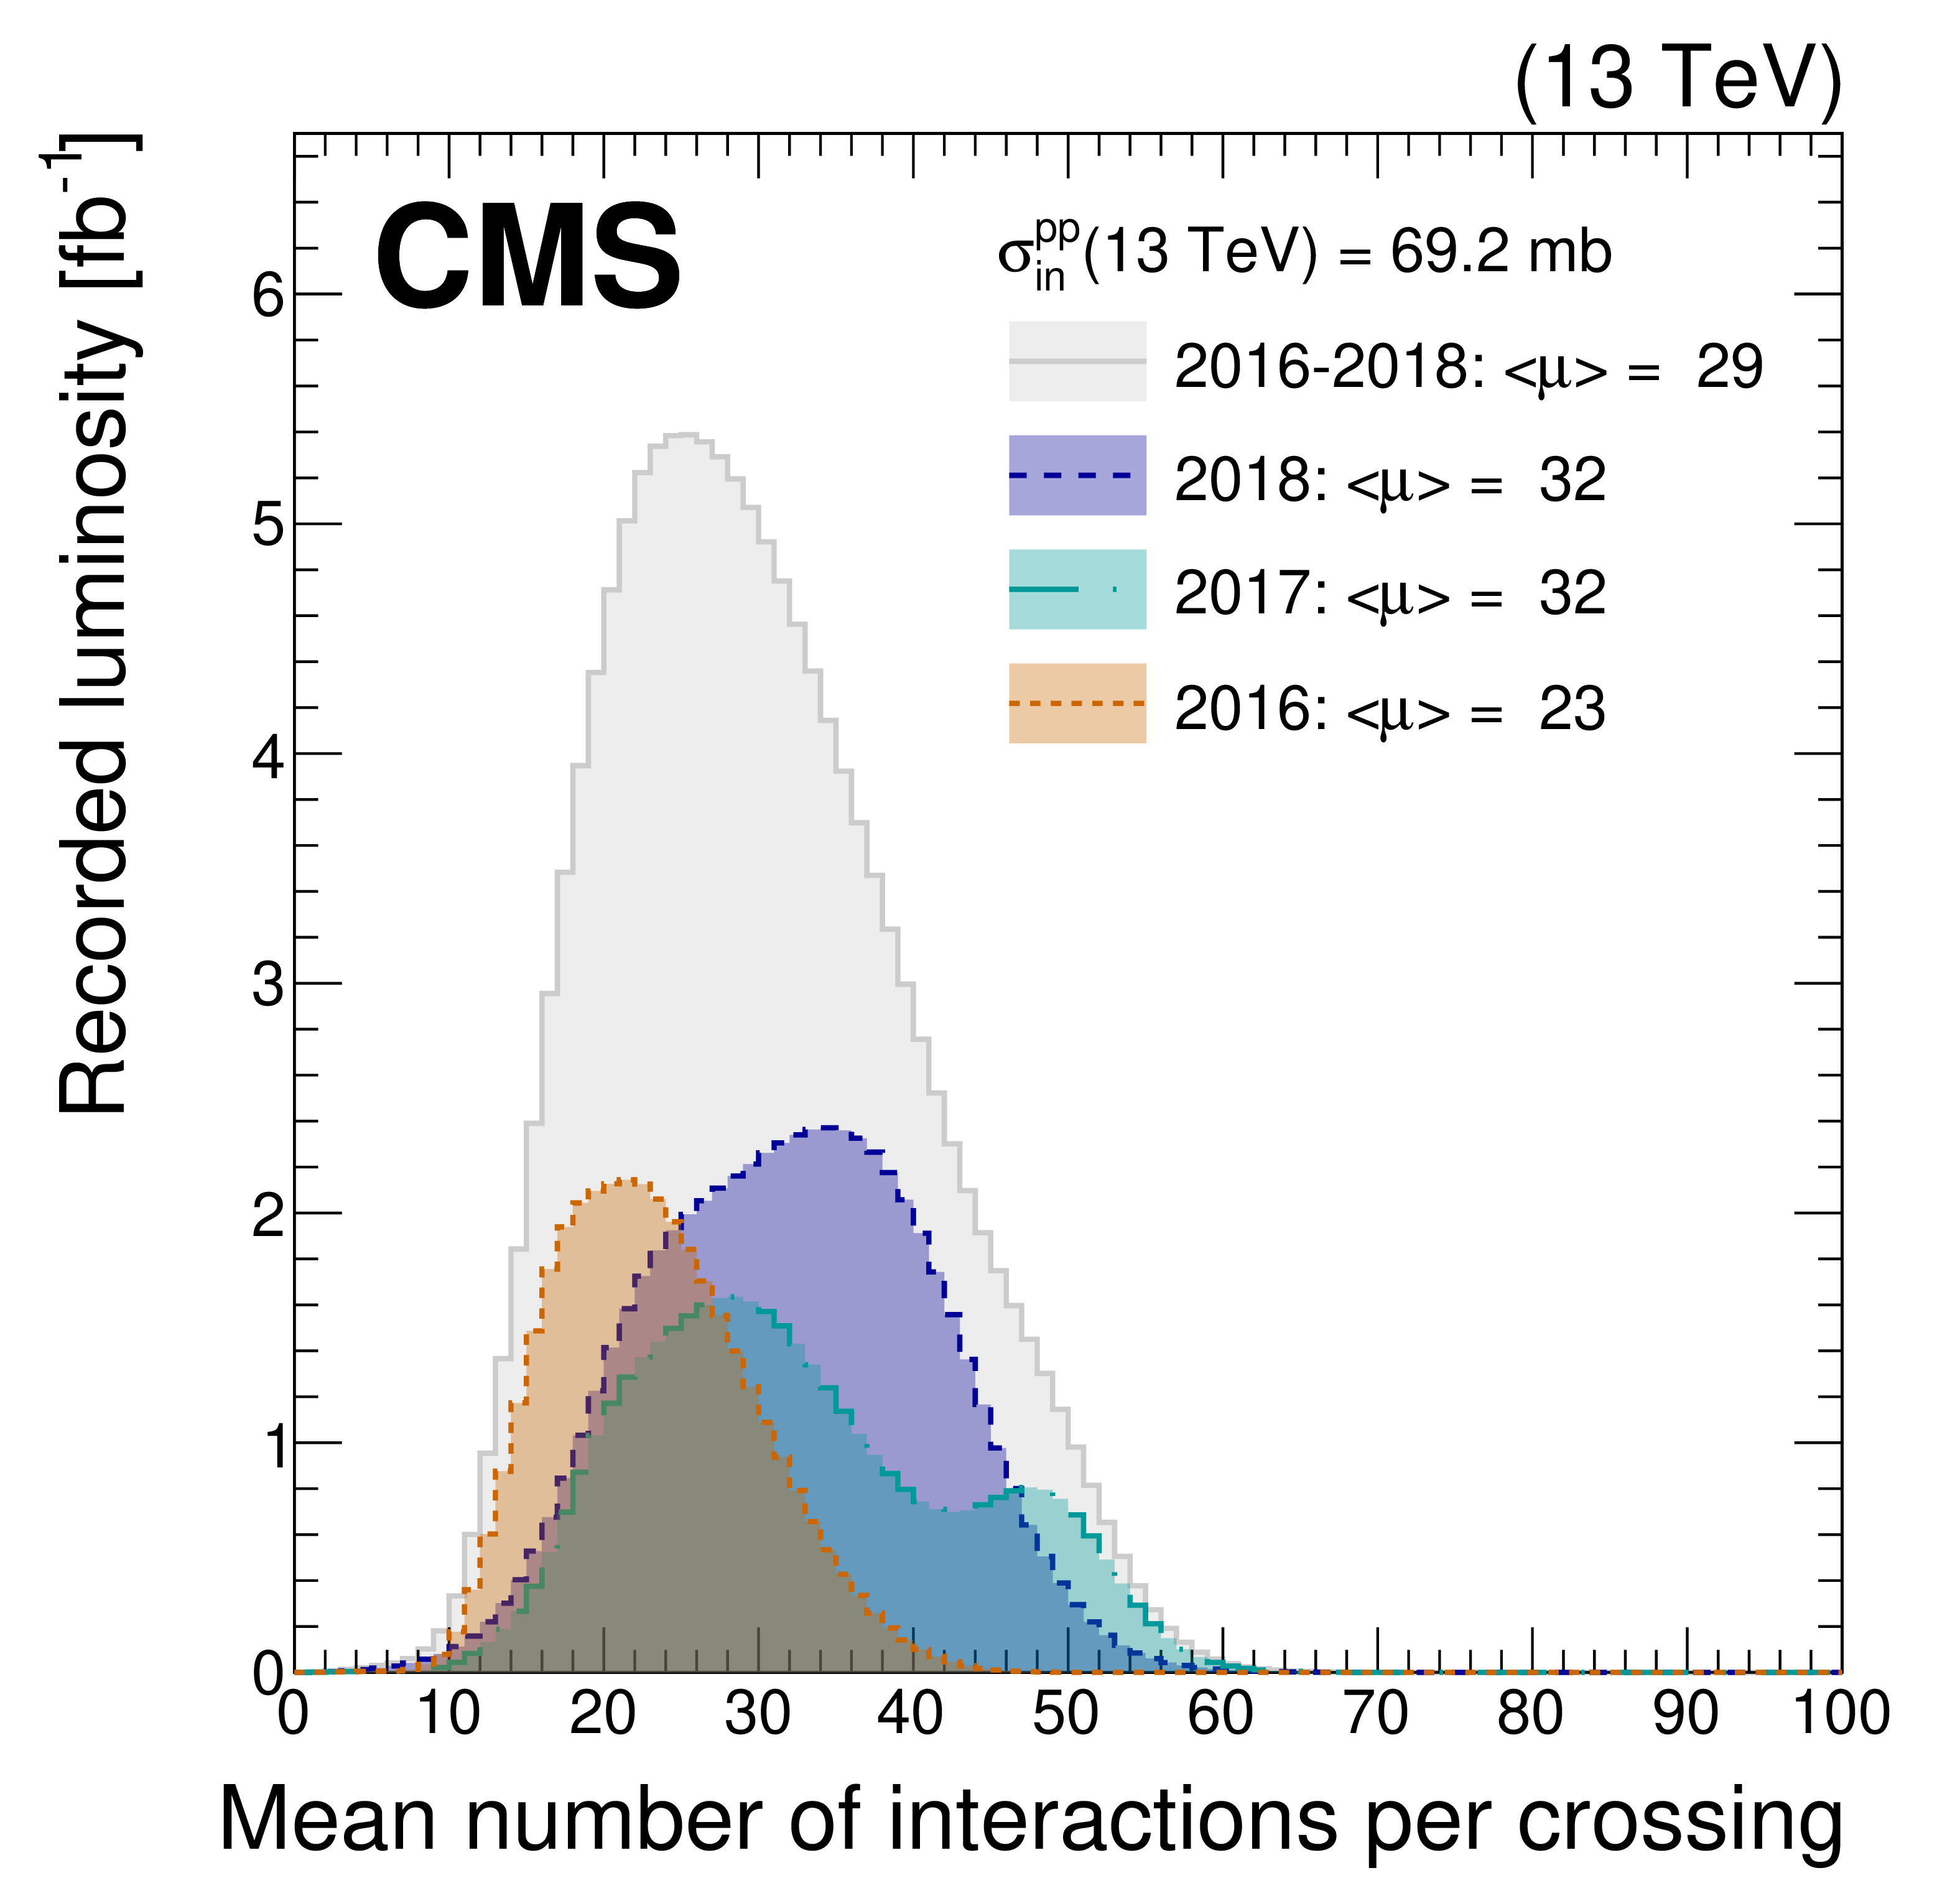
\includegraphics[width=8cm]{figures/ch-2-cern-cms/pileup-run-2-CMS-JME-18-001_Figure_001.png}
    \caption[Distribution of the mean number of inelastic collisions per bunch crossing (pileup) in data, for proton-proton collisions in 2016-2018]{Distribution of the mean number of inelastic collisions per bunch crossing (pileup) in data \cite{CMS-JME-18-001}, for proton-proton collisions in 2016 (\textit{dotted orange}), 2017 (\textit{dotted light blue}), 2018 (\textit{dotted dark blue}), and integrated over 2016-2018 (\textit{solid grey}). A cross-section of inelastic proton-proton collisions of 69.2 mbarns is assumed. In the running conditions of the High-Luminosity LHC, pileup will reach unprecedented levels of up to 200 per bunch crossing \cite{CERN-2020-010-HL-LHC-TDR}.}
    \label{fig:pileup-run-2}
\end{figure}

\section{The High-Luminosity LHC}
\label{section:HL-LHC}
The High-Luminosity LHC (HL-LHC) is a major upgrade of the LHC scheduled to take place in the late 2020s, that will increase the instantaneous luminosity by a factor of of five beyond the original design value, and the integrated luminosity by a factor of ten \cite{CERN-2020-010-HL-LHC-TDR}. This will be accomplished through accelerator technological advances: for instance, reduction of the interaction point $\beta^*$ from 0.55 m down to 0.15 m by installation of new final-focusing magnets, and improvements in the geometric luminosity loss factor $F \approx 1$ through the installation of crab cavities that optimize the orientation of colliding bunches. A further discussion of the HL-LHC upgrades for the CMS detector follows in Chapter \ref{chapter:ch-3:phase-2-upgrade-cms}.

\section{The CMS Detector}
\label{section:cms-detector}

The Compact Muon Solenoid (CMS) experiment was conceived to study proton-proton and lead-lead collisions at a center-of-mass energy of 14 TeV (5.5 TeV nucleon-nucleon) and at luminosities up to $10^{34}$ cm$^{-2}$ s$^{-1}$ ($10^{27}$ cm$^{-2}$ s$^{-1}$) \cite{CMS-2008-JINST-3-S08004} \cite{CERN-EP-2017-110}. Starting from the beam interaction region at the center of the CMS detector, particles first pass through a silicon pixel and strip tracker, in which charged-particle trajectories (tracks) and origins (vertices) are reconstructed from signals (hits) in the sensitive layers. The tracker is immersed in a high-magnetic-field superconducting solenoid that bends the trajectories of charged particles, allowing the measurement of their electric charge and momenta. Electrons and photons are then absorbed in an electromagnetic calorimeter (ECAL) comprised of lead-tungstate scintillating-crystals. The corresponding electromagnetic showers are detected as clusters of energy recording in neighboring cells, from which the direction and energy of the particles can be determined. Charged and neutral hadrons may initiate a hadronic shower in the ECAL as well, which is then fully absorbed in the hadron calorimeter (HCAL). The resulting clusters are used to estimate their direction and energies. Muons and neutrinos pass through the calorimeters with little to no interactions. Neutrinos escaped undetected; muons produce hits in additional gas-ionization chamber muon detectors housed in the iron yoke of the flux-return. A sketch of example particle interactions in a transverse slice of the CMS detector is shown in Fig. \ref{fig:sketch-cms-particle-interactions}. The collision data is recorded with the use of the Level-1 (L1) trigger (discussed in greater detail in \ref{section:phase-1-l1-trigger}), the High-Level Trigger (HLT), and data acquisition systems ensuring high efficiency in selecting physics events of interest. 

\begin{figure}[ht]
    \centering
    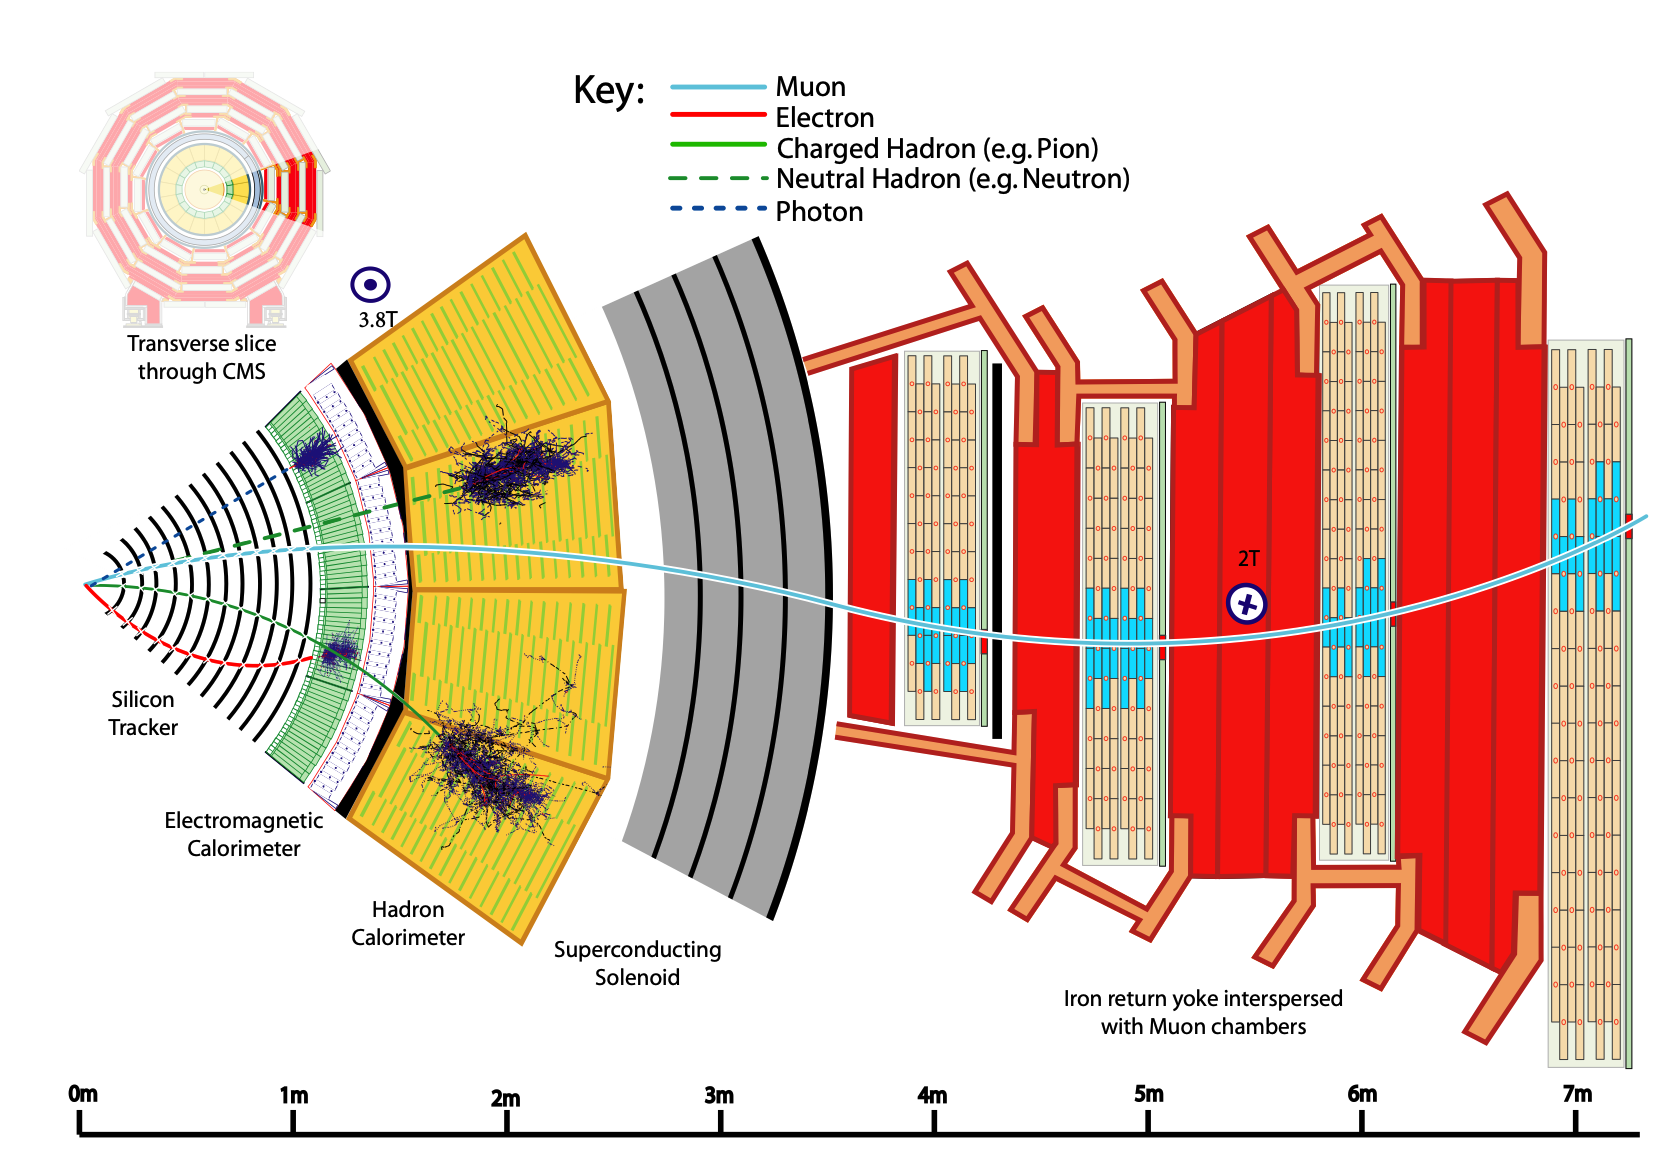
\includegraphics[width=11cm]{figures/ch-2-cern-cms/sketch-cms-particle-interactions.png}
    \caption[Sketch of particle trajectories of muons, electrons, charged and neutral hadrons, and photons in a transverse cross-section of the CMS detector.]{Sketch of particle trajectories of muons, electrons, charged and neutral hadrons, and photons in a transverse cross-section of the CMS detector \cite{CERN-EP-2017-110}.}
    \label{fig:sketch-cms-particle-interactions}
\end{figure}

CMS uses a right-handed coordinate system \cite{CMS-2008-JINST-3-S08004}. The origin is centered at the nominal collision point inside the experiment. The $x$ axis points towards the center of the LHC, and the $y$ axis points vertically upwards. The $z$ axis points along the beam direction. The azimuthal angle, $\phi$, is measured from the $x$ axis in the $x$-$y$ plane, and the radial coordinate in this plane is denoted by $r$. The polar angle, $\theta$, is measured from the $z$ axis. The pseudorapidity, $\eta$, is defined as $\eta = -\ln \tan(\theta/2)$. The momentum and energy transverse to the beam direction, denoted by $p_{T}$ and $E_{T}$ respectively, are computed from the $x$ and $y$ components. The momentum imbalance in the transverse plane is called the missing transverse momentum, and its magnitude is denoted by $E_{T}^{\text{miss}}$.

\section{Sub-detectors of CMS}
This section details the sub-detectors of CMS that operate to identify and precisely measure muons, electrons, photons, and jets over a large energy range. 

\subsection{Inner tracking system}

The CMS Tracker performs robust tracking and detailed vertex reconstruction in the 4 T magnetic field of the superconducting solenoidal magnet. The primary sensors used in the tracker are $p^+$ on $n$-bulk devices, which allow high voltage operation and are radiation-resistant \cite{CERN-LHCC-98-006} \cite{CERN-LHCC-2017-009-tracker-phase2-tdr}. The active envelope of the CMS Tracker extends to a radius of 115 cm, over a length of approximately 270 cm on each side of the interaction point \cite{CERN-LHCC-98-006}.
Charged particles in the region $|\eta| \lesssim 1.6$ benefit from the full momentum measurement precision. In this region, a charged particle with $p_T$ of 1000\GeV has a sagitta of $\sim 195$ $\mu$m. The Tracker acceptance extends further to $|\eta| = 2.5$, with a reduced radius of approximately 50 cm.

The high magnetic field of CMS causes low $p_{T}$ charged particles to travel in helical trajectories with small radii. The majority of events contain particles with a steeply falling $p_{T}$ spectrum, resulting in a track density which rapidly decreases at higher radii. 

A schematic view of the current Phase-1 CMS tracker \cite{CMS-TDR-011-pixel}, including the pixel detector, is shown in Fig. \ref{fig:phase-1-tdr-tracker-schematic}. The Phase-1 pixel detector consists of three barrel layers (BPIX) at radii of 4.4 cm, 7.3 cm, and 10.2 cm, and two forward/backward disks (FPIX) at longitudinal positions of $\pm$ 34.5 cm and $\pm$ 46.5 cm, and extending in radius from about 6 cm to 15 cm. These pixelated detectors produce 3D measurements along the paths of charged particles with single hit resolutions between 10-20 $\mu$m. 


\begin{figure}[ht]
    \centering
    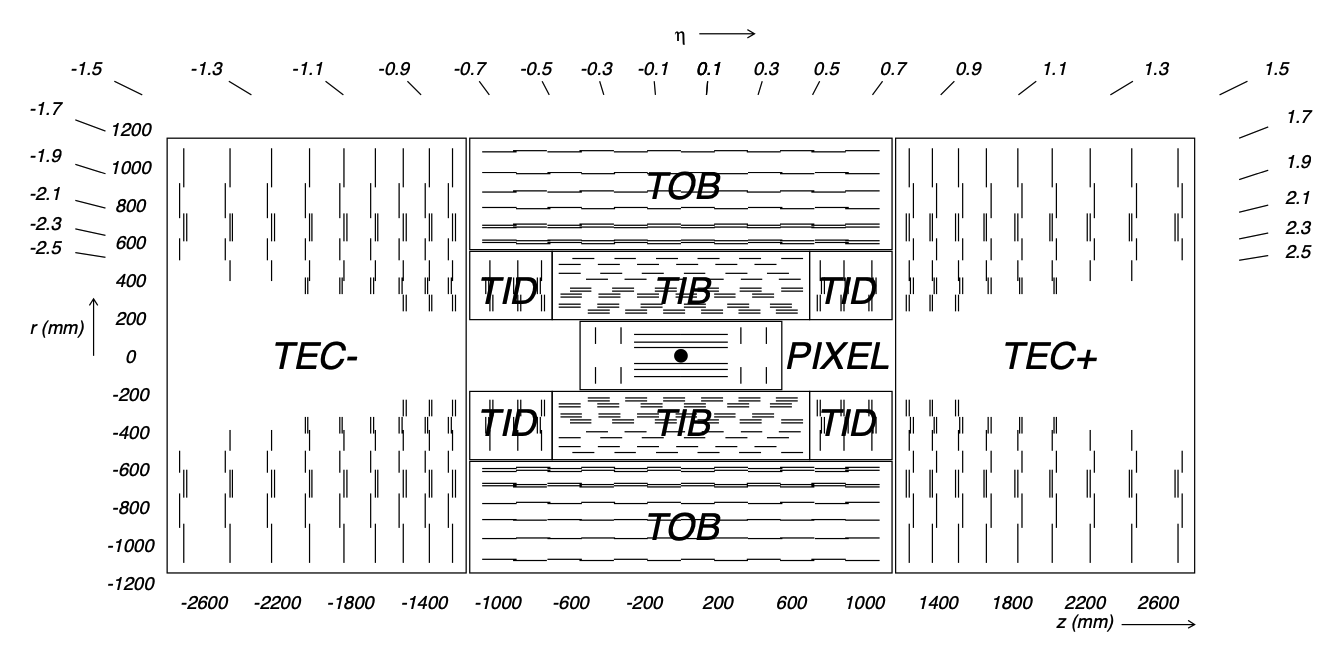
\includegraphics[width=11cm]{figures/ch-2-cern-cms/phase-1-tdr-tracker-schematic.png}
    \caption[Cross section of the current Phase-1 CMS tracker.]{Cross section of the current Phase-1 CMS tracker \cite{CMS-TDR-011-pixel}. Each line represents a detector module. Double lines indicate back-to-back modules which deliver two-dimensional (stereo) hits in the strip tracker.}
    \label{fig:phase-1-tdr-tracker-schematic}
\end{figure}

After the pixel and on their way out of the tracker, particles pass through the silicon strip tracker which reaches out to a radius of 130 cm (Fig. \ref{fig:phase-1-tdr-tracker-schematic}). The sensor elements in the strip tracker are single-sided $p$-on-$n$ type silicon micro-strip sensors \cite{CMS-2008-JINST-3-S08004}. The silicon strip detector consists of four inner barrel (TIB) layers assembled in shells, with two inner endcaps (TID), each composed of three small discs. The outer barrel (TOB) consists of six concentric layers. Two endcaps (TEC) close off the tracker on either end. 


\subsection{ECAL} 
The electromagnetic calorimeter (ECAL) of CMS measures electromagnetic energy deposits with high granularity. One of the driving criteria in the design was the capability of detecting the Standard Model Higgs boson decay to two photons (in fact, the channel in which the 125\GeV Higgs boson was discovered at CMS). 
ECAL is a hermetic homogeneous calorimeter comprised of 61,200 lead tungstate (PbWO$_4$) crystals mounted in the central barrel, with 7,324 crystals in each of the two endcaps \cite{CMS-2008-JINST-3-S08004}. A preshower detector is located in front of the endcap crystals. Avalanche photodiodes (APDs) are used as photodetectors in the barrel and vacuum phototriodes (VPTs) in the endcaps. 

The design of the ECAL is driven by the behaviour of high-energy electrons, which predominantly lose energy in matter via bremsstrahlung, and high-energy photons by $e^+ e^-$ pair production. The characteristic amount of matter traversed for these interactions is the radiation length $X^0$, usually measured in units of g cm$^-2$. The radiation length is also the mean distance over which a high-energy electron loses all but $1/e$ of its energy via bremsstrahlung \cite{workman_review_2022}. Thus high granularity in $\eta$ and $\phi$, and the length of the ECAL crystals, is designed to capture the shower of $e/\gamma$ produced by electrons and photons.

The barrel part of the ECAL (EB) covers the pseudorapidity range $|\eta| < 1.479$ \cite{CMS-2008-JINST-3-S08004}. The barrel granularity is 360-fold in $\phi$ and ($2 \times 85$)-fold in $\eta$. The crystal cross-section corresponds to approximately $0.0174 \times 0.0174$ in $\eta-\phi$ or $22 \times 22$ mm$^2$ at the front face of the crystal, and $26 \times 26$ mm$^2$ at the rear face. The crystal length is 230 mm, corresponding to 25.8 $X_0$.

The ECAL read-out acquires the signals of the photodetectors  \cite{CMS-2008-JINST-3-S08004}. At each bunch crossing, digital sums representing the energy deposit in a trigger tower, comprising $5 \times 5$ crystals in $\eta \times \phi$, are generated and sent to the Level-1 trigger system (detailed in Section \ref{section:phase-1-l1-trigger}).

\subsection{HCAL}
The hadronic calorimeter (HCAL) of CMS measures hadronic energy, which is key to characterizing the presence of apparent missing transverse energy which could arise from hadron jets and neutrinos or exotic particles \cite{CMS-2008-JINST-3-S08004}. A schematic of the components of HCAL are shown in Fig. \ref{fig:phase-1-HCAL-schematic}. The HCAL barrel (HB) and endcaps (HE) are located outside of the tracker and the ECAL, spanning a radius of 1.77 m (outer extent of ECAL) up to 2.95 m (inner extent of the magnet coil). An outer hadron calorimeter (HO) is placed outside the solenoid to complement the barrel calorimeter. Beyond $|\eta| = 3$, the forward hadron calorimeter (HF) at 11.2 m from the interaction point extend the pseudorapidity coverage to $|\eta| = 5.2$.

\begin{figure}[ht]
    \centering
    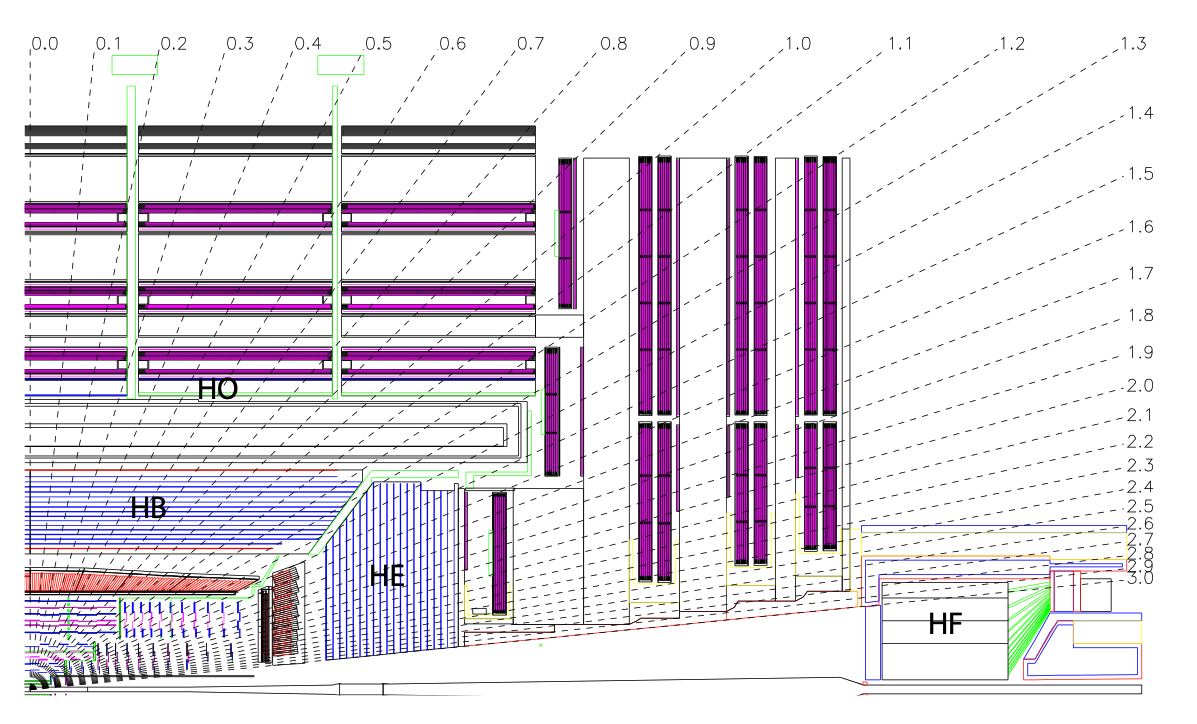
\includegraphics[width=11cm]{figures/ch-2-cern-cms/phase-1-HCAL-schematic.png}
    \caption[Longitudinal view of the CMS detector showing the hadron calorimeter barrel (HB), endcap (HE), outer (HO), and forward (HF) calorimeters.]{Longitudinal view of the CMS detector showing the hadron calorimeter barrel (HB), endcap (HE), outer (HO), and forward (HF) calorimeters from \cite{CMS-2008-JINST-3-S08004}.}
    \label{fig:phase-1-HCAL-schematic}
\end{figure}

The HB is a sampling calorimeter covering the pseudorapidity range $|\eta| < 1.3$ \cite{CMS-2008-JINST-3-S08004}. It consists of 36 identical azimuthal wedges which form two half-barrels (HB+ and HB-), with a segmentation of $(\Delta \eta, \Delta \phi) = (0.087, 0.087)$. The HE covers pseudorapidity $1.3 < |\eta| < 3$. The HB and endcap HE calorimeters are sampling calorimeters which use brass as the absorber and plastic scintillator as the active material. Light from the plastic scintillator is wavelength-shifted and captured in optic fibers which are read out by front-end electronics \cite{CMS-TDR-010-2012}. 

In the central pseudorapidity region, the combined stopping power of EB plus the HB is insufficient to contain hadron showers \cite{CMS-2008-JINST-3-S08004}. To ensure adequate sampling depth, the hadron calorimeter is extended with a tail catcher, the HO. The size and position of the tiles are designed to roughly map the layers of the HB to make towers with the same granularity of $0.087 \times 0.087$ in $\eta$ and $\phi$. HO uses the same active material as the HB and HE calorimeters, but uses the steel return yoke and magnet material of CMS as absorbers \cite{CMS-TDR-010-2012}. 


The HF is a Cherenkov calorimeter based on a steel absorber and quartz fibers which run longitudinally through the absorber and collect Cherenkov light, primarily from the electromagnetic component of showers developed in the calorimeter \cite{CMS-TDR-010-2012}. Photomultiplier tubes are used to  collect light from the quartz fibers. The HF is designed to survive in the harsh radiation conditions and high particle flux of the forward region. On average, 760\GeV per proton-proton interaction is deposited into the two forward calorimeters, compared to only 100\GeV for the rest of the detector \cite{CMS-2008-JINST-3-S08004}. Furthermore, this energy has a pronounced maximum at the highest rapidities.

\subsection{Muon detectors}
The CMS muon system is designed to have the capability of reconstructing the momentum and charge of muons over the kinematic range of the LHC, since muons are a powerful handle on signatures of interesting processes over the high background rate of the LHC \cite{CMS-2008-JINST-3-S08004}. For instance, the decay of the Standard Model Higgs boson into $ZZ$, which in turn decay to 4 leptons, can be reconstructed with high 4-particle mass resolution if all the leptons are muons, since muons are less affected than electrons by radiative losses in the tracker material. 

The muon system consists of a cylindrical barrel section and two planar endcap regions \cite{CMS-2008-JINST-3-S08004}. The barrel muon detector consists of drift tube (DT) chambers covering the pseudorapidity region $|\eta| < 1.2$ (Fig. \ref{fig:phase-1-muon-barrel-DT-schematic}). The DTs can be used as tracking detectors due to the barrel region's characteristic low neutron-induced backgrounds, low muon rate, and relatively uniform 4T magnetic field contained in the steel yoke. 

\begin{figure}[ht]
    \centering
    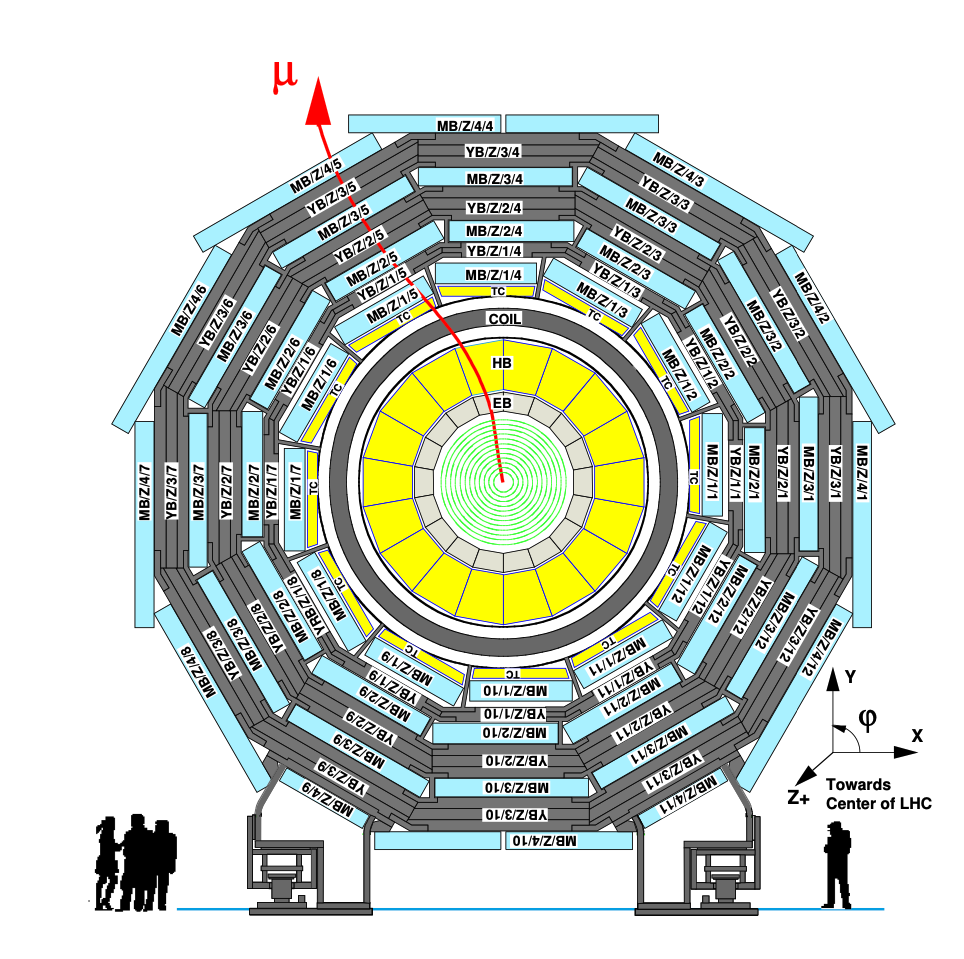
\includegraphics[width=11cm]{figures/ch-2-cern-cms/phase-1-muon-barrel-DT-schematic.png}
    \caption[Layout of the CMS barrel muon drift tube (DT) chambers in one of the five wheels.]{Layout of the CMS barrel muon drift tube (DT) chambers in one of the five wheels from \cite{CMS-2008-JINST-3-S08004}. The DTs are organized in 12 sectors of the yoke barrel (YB). In each of the 12 sectors of the yoke, there are 4 muon chambers per wheel (MB1, MB2, MB3, and MB4).}
    \label{fig:phase-1-muon-barrel-DT-schematic}
\end{figure}

In the two endcap regions, the muon rates and background levels are high and the magnetic field is large and non-uniform \cite{CMS-2008-JINST-3-S08004}. Here, the muon system uses cathode strip chambers (CSCs) to identify muons between $0.9 < |\eta| < 2.4$. The cathode strips of each chamber run radially outwards and provide a precision measurement in the $r-\phi$ bending plane. The anode wires run approximately perpendicular to the strips and are read out in order to measure $\eta$ and the beam-crossing time of a muon. 

% 2008 JINST 3 S08004, page 164
In addition to the DT and CSC, a dedicated trigger system consisting of resistive plate chambers (RPCs) in the barrel and endcap regions provide a fast, independent, and highly-segmented trigger with a sharp $p_T$ threshold over a large portion of the pseudorapidity range ($|\eta| < 1.6$) of the muon system \cite{CMS-2008-JINST-3-S08004}. RPCs have good time resolution but coarser position resolution compared to the DTs or CSCs. The RPCs also play a role in resolving ambiguities in reconstructing tracks from multiple hits in a chamber. 

\subsection{The Level-1 Trigger}
\label{section:phase-1-l1-trigger}
The design performance of the LHC corresponds to an instantaneous luminosity of $10^{34}$ cm$^{-2}$ s$^{-1}$ with a 25 ns bunch crossing rate, giving an average pile-up (number of simultaneous events) of 25 per bunch crossing \cite{CMS-TDR-012}. The large number of minimum bias events per bunch crossing, combined with the small cross-sections of possible physics discovery signatures, necessitates a sophisticated event selection system for filtering this large event rate, as it is impossible to save all events. This data filtering system is implemented by CMS in two stages. The first stage is the Level-1 (L1) Trigger, which is deployed in custom electronic hardware systems and is responsible for reducing the event rate to around 100 kHz. The second stage is the High-Level Trigger (HLT) which is described in Section \ref{section:phase-1-high-level-trigger}. This section describes the Phase-1 configuration of the Level-1 Trigger.


The L1 Trigger data flow of Phase-1 is shown in Fig. \ref{fig:phase-1-level-1-trigger-dataflow} \cite{CMS-TDR-012}, with organization into the L1 calorimeter trigger, the L1 muon trigger, and the L1 global trigger. 

\begin{figure}[ht]
    \centering
    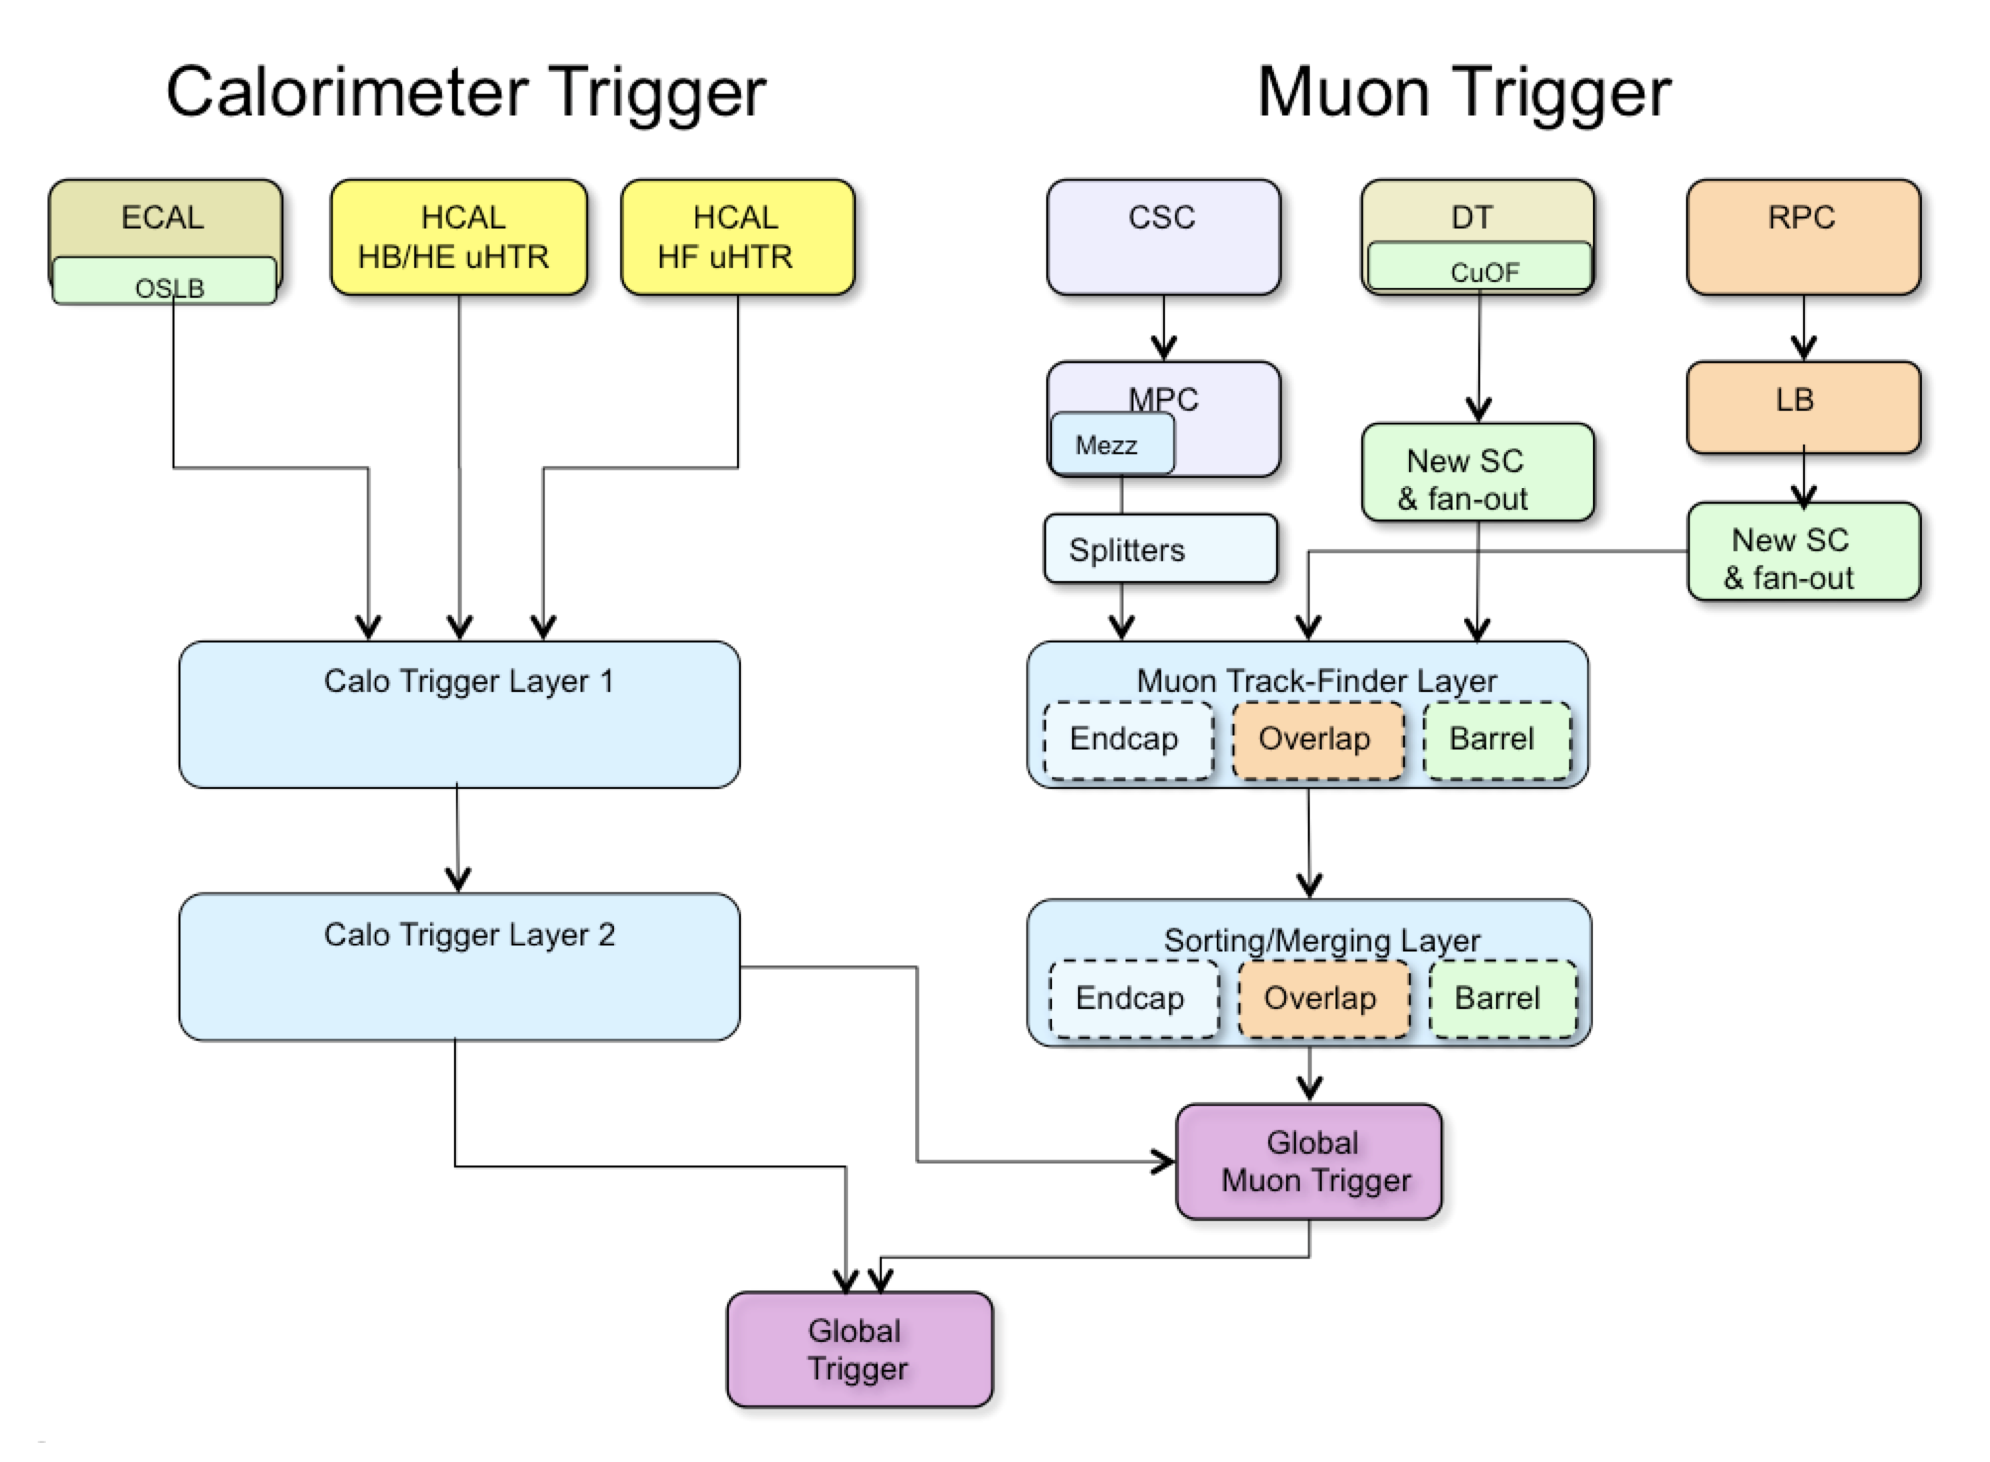
\includegraphics[width=11cm]{figures/ch-2-cern-cms/phase-1-level-1-trigger-dataflow.png}
    \caption[Dataflow for the Phase-1 Level-1 Trigger.]{Dataflow for the Phase-1 Level-1 Trigger \cite{CMS-TDR-012}, which is implemented in custom hardware and is responsible for reducing the event rate from the LHC bunch crossing frequency of 400 MHz (bunch crossings every 25 ns) to a maximum rate of 100 kHz. In Phase-1, the Level-1 Trigger has access to information from the calorimeter and muon detectors.}
    \label{fig:phase-1-level-1-trigger-dataflow}
\end{figure}

The L1 calorimeter trigger begins with trigger tower energy sums formed by the ECAL, HCAL, and HF Trigger Primitive Generator (TPG) circuits from the individual calorimeter cell energies. In the original configuration, the ECAL energies were accompanied by a bit indicating the transverse extent of the electromagnetic energy deposits, and the HCAL energies were accompanied by a bit indicating the presence of minimum ionizing energy \cite{CERN-LHCC-2000-038}. Between Long Shutdowns 1 and 2 (LS1 and LS2), HF was upgraded to provide finer granularity information to the trigger, and the HCAL barrel and endcap front-end electronics were upgraded to provide high-precision timing information and depth segmentation information. 

In the original design of the L1 calorimeter trigger, the trigger primitives are processed by the Regional Calorimeter Trigger (RCT, upgraded to Calo Layer 1 after LS2) which finds isolated and non-isolated electron/photon candidates \cite{CMS-TDR-012}. At this stage, electrons/photons candidates are treated together since they cannot be definitively distinguished at this stage due to lack of tracking information in the L1 trigger. The Global Calorimeter Trigger (GCT, upgraded to Calo Layer 2 after LS2) sorts further the candidate electrons/photons, finds jets (classified as central, forward, and tau) using the $E_T$ sums and performs calibration of the clustered jet energies, and calculates global quantities such as missing $E_T$. It sends the top four candidates of each type to the global trigger (GT) \cite{CMS-TDR-012}.

Each of the L1 muon triggers has its own trigger logic \cite{CERN-LHCC-2000-038}. The RPC strips are connected to a Pattern Comparator Trigger (PACT), which forms trigger segments that are used to build tracks and calculate $p_{T}$. The RPC logic also provides some hit data to the CSC trigger system to resolve ambiguities caused by two muons in the same CSC. The CSCs form local charged tracks (LCTs) from the cathode strips, which are combined with the anode wire information. LCTs are combined into full muon tracks and assigned $p_{T}$ values. 

The Global Muon Trigger (GMT) sorts the RPC, DT, and CSC muon tracks, converts these tracks to the same $\eta$, $\phi$, and $p_{T}$ scale, and validates the muon sign \cite{CERN-LHCC-2000-038}. It improves the trigger efficiency by merging muon candidates that were detected in two complementary sub-systems (i.e. DT+RPC, or CSC+RPC). The GMT also contains logic to correlate the found muon tracks with an $\eta-\phi$ grid of quiet calorimeter towers to determine if the muons are isolated, as well as logic to remove duplicate candidates originating in the overlap regions from both DT and CSC systems. The final collection of muons are sorted based on their initial quality, correlation, and $p_{T}$, and the top four muons are sent to the Global Trigger \cite{CERN-LHCC-2000-038}. 

Information from the GCT and GT are sent to the Global Trigger (GT), which makes the Level-1 Accept (L1A) decision to either discard or accept the bunch crossing \cite{CERN-LHCC-2000-038}. This is accomplished by sorting ranked trigger objects that are accompanied by positional information in $\eta$ and $\phi$, permitting the trigger to applying criteria with thresholds that can vary based on the location of the trigger objects, and/or to require trigger objects to be close to or opposite from each other. The GT L1A decision arrives at the detector front end with a 3.8 $\mu$s latency after the interaction at a rate which is required to be less than 100 kHz, and triggers a full readout of the detector for further processing.



\subsection{The High-Level Trigger}
\label{section:phase-1-high-level-trigger}
The HLT is implemented in software running on a large computer farm of fast commercial processors \cite{CMS-TDR-022-HLT} \cite{Foudas:2008dt}. The algorithms in HLT have access to full data from all CMS sub-detectors, including the tracker, with full granularity and resolution. The HLT reconstruction software is similar to what is used offline for full CMS data analysis. As a result, the HLT can calculate quantities with a resolution comparable to the final detector resolution, compared to the L1 Trigger. The HLT performs more computationally-intensive algorithms, such as combining tau-jet candidates in the calorimeter with high-$p_T$ stubs in the tracker, to form a hadronic tau trigger. The maximum HLT input rate from the L1 Trigger is 100 kHz, and the HLT output rate is approximately 100 Hz. 

The HLT contains trigger paths, each corresponding to a dedicated trigger \cite{twiki_SoftwareGuide_HLT}.  A path consists of several steps implemented as software modules. Each HLT trigger path must be seeded by one or more L1 trigger bits: the first module always looks for a L1 seed, consisting of L1 bit(s) and L1 object(s). Each module performs a well-defined task such as unpacking (raw to digitized quantities), reconstruction of physics objects (electrons, muons, jet, missing transverse energy, etc.), making intermediate decisions that trigger more detailed reconstruction modules, and calculating the final decision for the trigger path. If an intermediate filter decision is negative, the rest of the path is not executed, and the trigger rejects the event.


\subsection{Particle reconstruction}
To build a description of the physics objects present in the particle collision, the basic elements from the detector layers (tracks and clusters of energy) are correlated to identify each particle in the final state. Measurements from different sub-detectors are combined to reconstruct the particle properties. This approach is called particle-flow (PF) reconstruction \cite{CERN-EP-2017-110}. Key to the success of the PF reconstruction is the fine spatial granularity of the detector layers. Coarse-grained detectors can cause the signals from different particles to merge, especially within jets. However, if the subdetectors are sufficiently segmented to separate individual particles, it becomes possible to produce a global event description that identifies all physics objects with high efficiencies and resolution.

\subsection{Data storage and computational infrastructure}

The LHC generates over 15 petabytes (15 million gigabytes) of data every year, necessitating a flexible computing system that can be accessed by researchers working at the four main LHC experiments: ALICE, ATLAS, CMS, and LHCb. The Worldwide LHC Computing Grid (WLCG) \cite{computing-Worldwide:1997398} is a global collaboration of computer centers that links thousands of computers and storage systems in over 170 centers across 41 countries. These centers are arranged in ``tiers'', and provide near real-time access to users processing, analyzing, and storing LHC data. One of the final stages of data analysis at LHC experiments is large-scale data processing taking place over distributing computing, for instance, with the use of Condor \cite{condor-article}, a distributed, scalable, flexible batch processing system which accepts a computing job, allocates a resource to it, executes it, and returns the result back to a user transparently. 
 


\chapter{The Phase-2 Upgrade of CMS}
\label{chapter:ch-3:phase-2-upgrade-cms} 
This chapter gives an overview of the High-Luminosity LHC upgrade of the LHC in Section \ref{section:hl-lhc}, and the upgrades for the Phase-2 CMS Level-1 (L1) Trigger in Section \ref{section:phase-2-l1t}. One of the major upgrades is the new availability of calorimeter crystal-level information to the L1 calorimeter trigger, compared to the current trigger which only has access to tower-level information (a tower being 5 by 5 in crystals). To capitalize on the increased spatial granularity of this information, an upgraded algorithm is presented which reconstructs and identifies electron and photon candidates in the the Layer-1 Calorimeter Trigger. A description of the algorithm and a validation of its performance in Phase-2 conditions is given in Section \ref{section:standalone_barrel_calo_egamma}.

\section{The High-Luminosity LHC}
\label{section:hl-lhc}
In order to sustain and extend the LHC's physics discovery program and maintain operability for a decade or more, the LHC is undergoing a major upgrade to the High-Luminosity LHC (HL-LHC). In its final configuration, the HL-LHC will deliver a peak luminosity of $7.5 \times 10^{34}$ cm$^{-2}$ s$^{-1}$, potentially leading to total integrated luminosity of 4000 fb$^{-1}$ after ten years of operations, scheduled to begin in 2027~\cite{CMS-TDR-021}. This integrated luminosity is about ten times the predicted luminosity reach of the LHC in its initial configuration. To enable the CMS experiment to continue operations and data-taking and to maximize the discovery potential of the unprecedented amount of data, the CMS detector is undergoing Phase-2 upgrades in order to perform high-precision measurements and searches for physics beyond the Standard Model in the intense running conditions of the HL-LHC. 

\section{The Phase-2 Level-1 Trigger}
\label{section:phase-2-l1t}
To achieve the goals of the HL-LHC program and to ensure the collection of information-rich datasets in the HL-LHC, the Phase-2 upgrade of the CMS Level-1 Trigger~\cite{CMS-TDR-021} must be upgraded in conjunction with the CMS sub-detectors and their readouts, to maintain physics selectivity. The HL-LHC will produce an intense hadronic environment corresponding to 200 simultaneous collisions per beam crossing, necessitating comprehensive upgrades of the trigger system outlined below.

In order to cope with the increased pile-up and high occupancies of the HL-LHC, the latency of the L1 trigger system (time available to produce a L1 Accept signal) will be increased significantly from 3.8 $\mu$s to 12.5 $\mu$s, with an increased maximum output bandwidth of 750 kHz~\cite{CMS-TDR-021}. With the increased latency, in addition to information from calorimeters and muon detectors (as in the Phase-1 system), information from the new tracker and high-granularity endcap calorimeter can also be included at L1 for the first time. This is illustrated in the functional diagram of the architecture of the Phase-2 trigger system in Fig. \ref{fig:phase-2-l1-architecture}. 

\begin{figure}[ht]
    \centering
    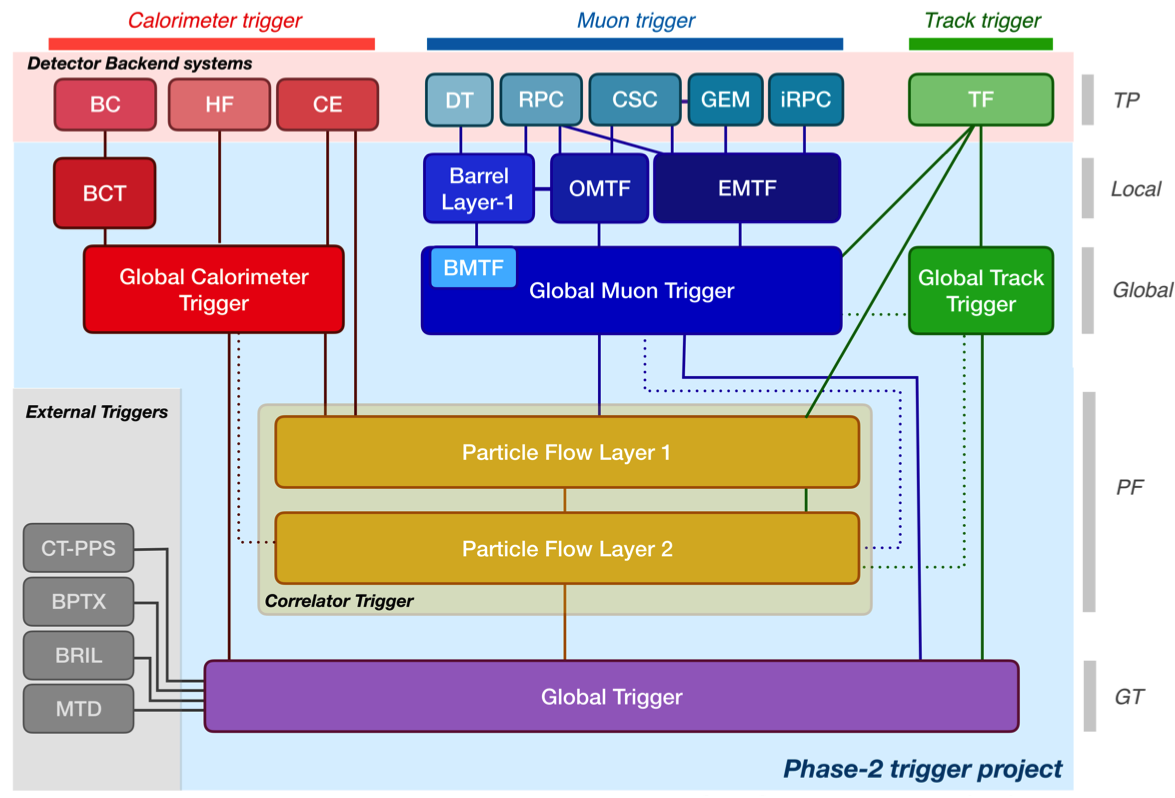
\includegraphics[width=15cm]{figures/ch-3-phase2/phase-2-l1-architecture.png}
    \caption[Functional diagram of the CMS L1 Phase-2 upgraded trigger design.]{Functional diagram of the CMS L1 Phase-2 upgraded trigger design~\cite{CMS-TDR-021}, showing the four trigger paths: calorimeter, muon, track, and Particle Flow. For the first time, tracking information will be available as early as the L1 Trigger.}
    \label{fig:phase-2-l1-architecture}
\end{figure}

The key feature of the Phase-2 L1 Trigger is the introduction of a correlator layer, where algorithms produce higher-level trigger objects by combining information from sub-detectors, with a selectivity approaching that of offline reconstruction in the HLT~\cite{CMS-TDR-021}. Four independent data processing paths (grouped together in Fig. \ref{fig:phase-2-l1-architecture}) are implemented: tracking, calorimetry, muon systems, and particle-flow techniques:
\begin{itemize}
    \item \textbf{Calorimeter Trigger path:} (\textit{red}, Fig. \ref{fig:phase-2-l1-architecture}) A barrel calorimeter trigger (BCT) and the HGCAL backend are used to process crystal-level information from the calorimeters to produce high-resolution clusters and identification variables used for later processing. Outputs from the BCT, HGCAL, and the HF are sent to a global calorimeter trigger (GCT), where calorimeter-only objects such as $e/\gamma$ candidates, hadronically decaying tau lepton candidates, jets, and energy sums are built.
    \item \textbf{Track Trigger path:} (\textit{green}, Fig. \ref{fig:phase-2-l1-architecture}) Tracks from the Outer Tracker are reconstructed in the track finder (TF) processors as part of the detector backend. A global track trigger (GTT) will reconstruct the primary vertices of the event, along with tracker-only based objects, such as jets and missing transverse momentum.
    \item \textbf{Muon Trigger path:} (\textit{blue}, Fig. \ref{fig:phase-2-l1-architecture}) Trigger primitives are processed by muon track finder algorithms, again separated into the barrel (barrel muon track finder, BMTF), overlap (overlap muon track finder, OMTF), and endcap (endcap muon track finder, EMTF). Standalone muons and stubs containing information such as position, bend angle, and timing, as well as L1 tracks, are sent to the global muon trigger (GMT).
    \item \textbf{Particle-Flow Trigger path:} (\textit{yellow}, Fig. \ref{fig:phase-2-l1-architecture}) The correlator trigger (CT) aims to approach the performance of offline Particle Flow, and is implemented in two layers. ``Layer-1'' produces the particle-flow candidates from matching calorimeter clusters and tracks. ``Layer 2'' builds and sorts final trigger objects and applies additional identification and isolation criteria.
\end{itemize}

The outputs from the above trigger paths are combined in the Global Trigger (GT) (\textit{purple}, Fig. \ref{fig:phase-2-l1-architecture}), which calculates the final trigger decision (Level-1 Accept), transmitting it to the Trigger Control and Distribution System (TCDS), which distributes it to the detector backend systems, initiating the readout to the DAQ. The GT also provides the interface to external triggers (\textit{grey}, Fig. \ref{fig:phase-2-l1-architecture}), such as triggers for the precision proton spectrometer (PPS), beam position and timing monitors (BPTX), and luminosity and beam monitoring (BRIL) detectors~\cite{CMS-TDR-021}. The design of the Phase-2 Level-1 Trigger allows for future inclusion of triggering information, for instance information about minimum ionizing particles (MIPs) from the MIP Timing Detector (MTD)~\cite{CERN-LHCC-2017-027}.

\section{Standalone Barrel Calorimeter electron/photon reconstruction}
\label{section:standalone_barrel_calo_egamma}
The reconstruction and identification of electrons and photons ($e/\gamma$) begin with the trigger primitives of the barrel ECAL and HCAL detectors and endcap HGCAL calorimeters, covering the pseudorapidity region $|\eta| < 3$. The barrel and endcap regions of the detector are intrinsically different enough to warrant different approaches to $e/\gamma$ reconstruction. This work presents a firmware-based emulator for the standalone $e/\gamma$ reconstruction in the barrel calorimeter (Fig. \ref{fig:phase-2-summary-trigger-TP-algo-physics}). ``Standalone" refers to the fact that the tracker information is not used in this particular reconstruction chain. This firmware-based emulator is based on the parallelized, computational logic that will be deployed in the firmware of the Phase-2 Level-1 trigger. The emulator uses fixed-precision integers to represent all values, such as in the computation of cluster energies, and closely mimics the firmware logic which uses arrays and performs computations in flattened loops. It represents an improved, more realistic understanding of the trigger, compared to the previous emulator which used idealized logic such as vector operations, and floats to represent all values~\cite{CMS-TDR-021}.

\begin{figure}[ht]
    \centering
    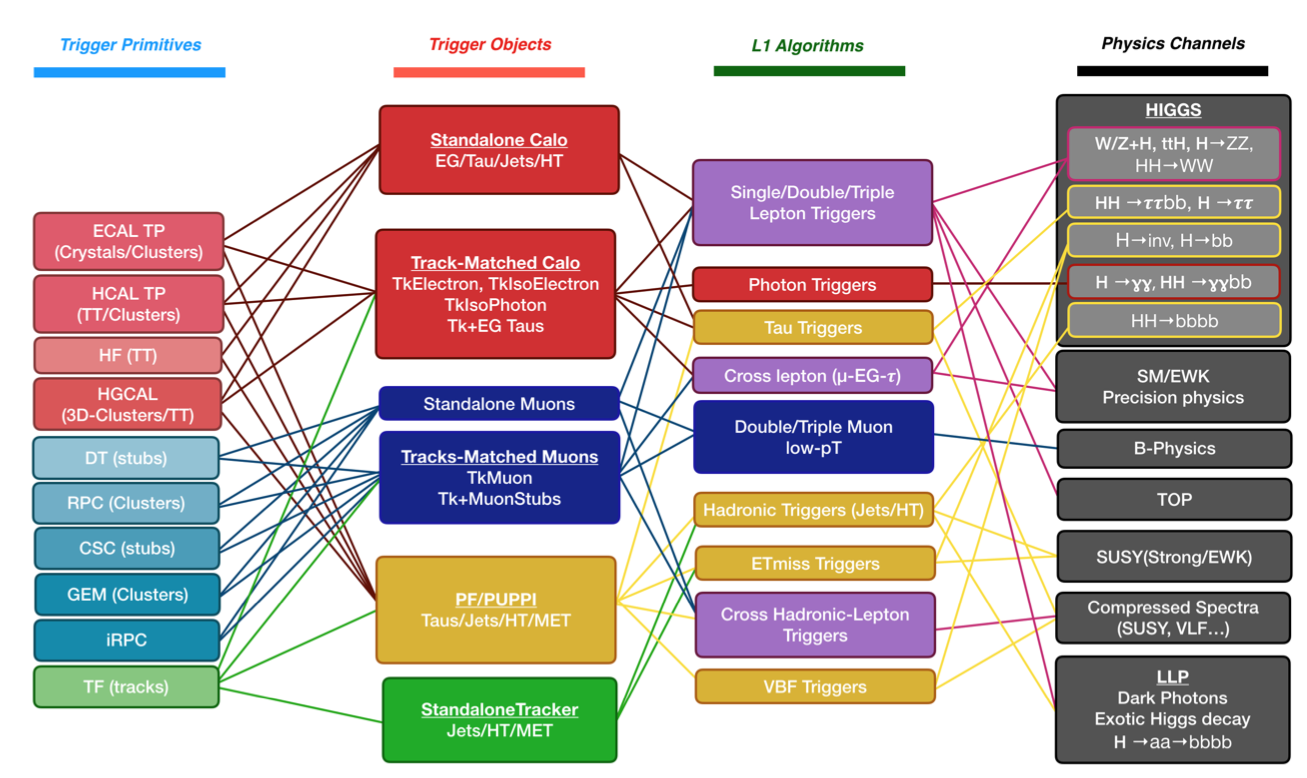
\includegraphics[width=15cm]{figures/ch-3-phase2/phase-2-summary-trigger-TP-algo-physics.png}
    \caption[Summary of the links between the trigger primitives, the trigger objects, the Level-1 algorithms, and the physics channels in the Phase-2 menu.]{Summary of the links between the trigger primitives (\textit{first column}), the trigger objects (\textit{second column}), the Level-1 algorithms used in the menu (\textit{3rd column}), and the physics channels (\textit{4th column}), from~\cite{CMS-TDR-021}, where a full description of the Phase-2 L1 algorithms can be found. This work focuses on developments for the Standalone Calorimeter electron and photon ("EG") reconstruction algorithm.}
    \label{fig:phase-2-summary-trigger-TP-algo-physics}
\end{figure}

\subsection{Electron/photon standalone barrel procedure}
% https://cds.cern.ch/record/2714892/files/CMS-TDR-021.pdf  
% Section 2.2.1, on page 36-37
In Phase-2, the upgrade of both on-detector and off-detector electronics of the barrel calorimeters' trigger primitive generator (TPG) will enable the streaming of single crystal data from the on-detector to the backend electronics. Currently in Phase-1, the ECAL and HCAL TPGs is restricted to providing lower-granularity information of trigger tower sums of $5 \times 5$ crystals to the Level-1 Trigger~\cite{CMS-TDR-021}. A schematic of the geometry of the ECAL barrel in the Phase-2 Regional Calorimeter Trigger (RCT) is shown in Fig. \ref{fig:phase-2-rct-cards-schematic}. The barrel is spanned by 36 RCT cards, each spanning $17 \times 4$ towers in $\eta \times \phi$. Each RCT card is subdivided into five ``regions'' as shown in Fig. \ref{fig:phase-2-one-rct-card-schematic-landscape}.  After initial clustering and processing, the outputs of the RCT card are sent to the Global Calorimeter (GCT) trigger, which is processed in three cards as shown in Fig. \ref{fig:phase-2-gct-cards-schematic}. The reconstruction algorithm is detailed below.
\begin{figure}[!ht]
    \centering
    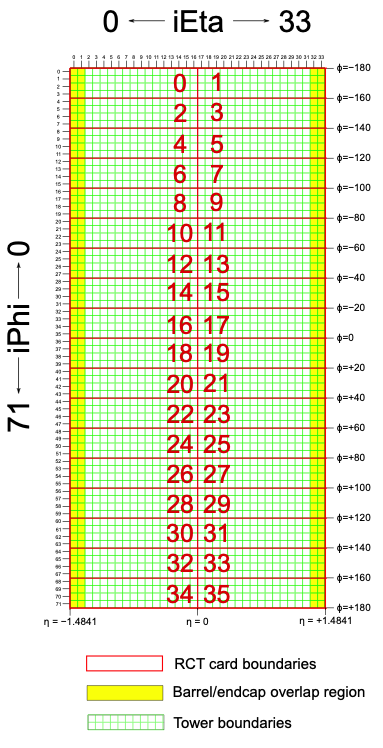
\includegraphics[width=5cm]{figures/ch-3-phase2/phase-2-rct-cards-schematic.png}
    \caption{Schematic of the geometry of the Phase-2 ECAL barrel in the Regional Calorimeter Trigger (RCT), showing the division of the barrel region into 36 Regional Calorimeter Trigger (RCT) cards (\textit{red}). Each card spans $17 \times 4$ towers in $\eta \times \phi$ (\textit{green}), and each tower is $5\times 5$ in single crystals in $\eta \times \phi$. Towers in the overlap region (\textit{shaded yellow}) are read out to both the barrel and endcap.}
    \label{fig:phase-2-rct-cards-schematic}
\end{figure}


\begin{figure}[ht]
    \centering
    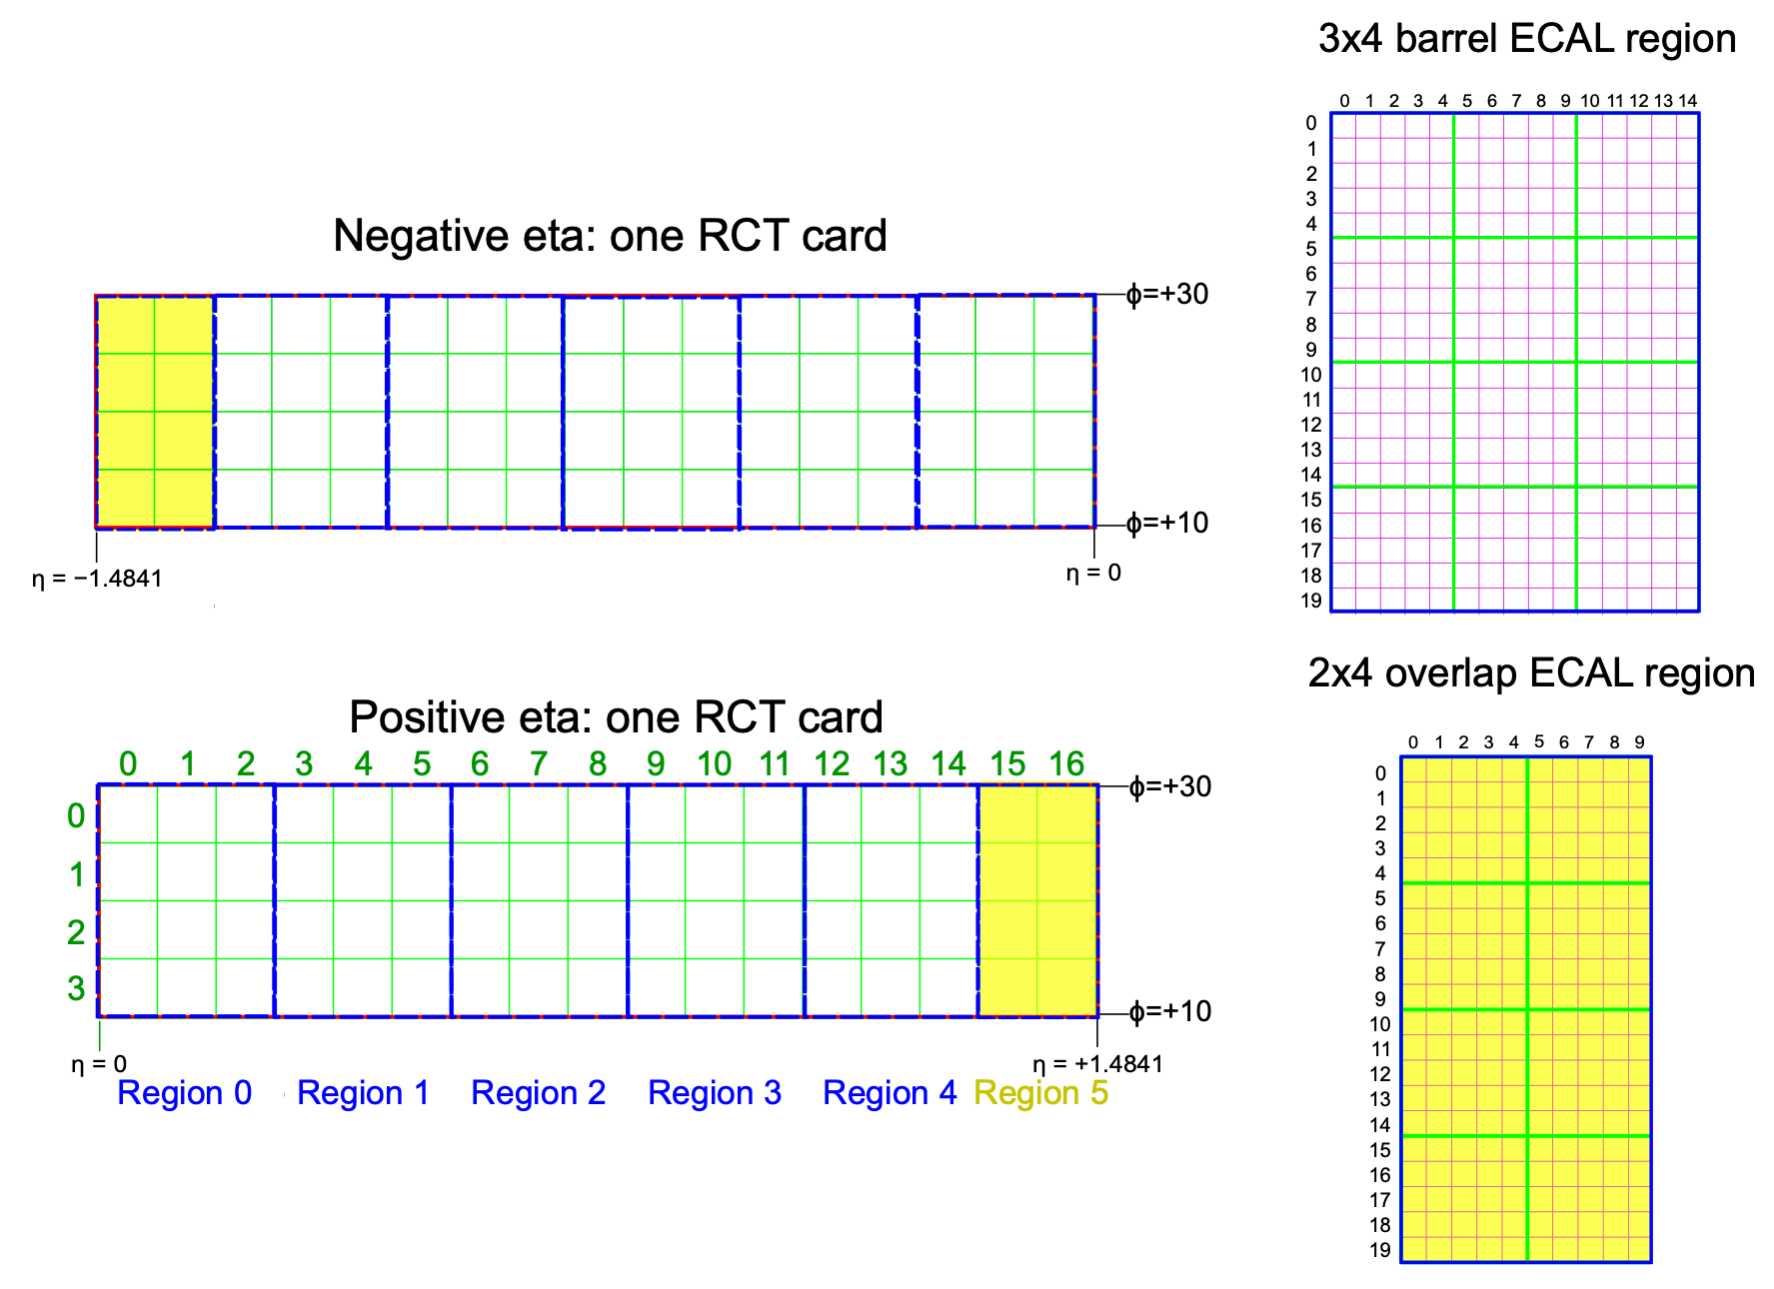
\includegraphics[width=11cm]{figures/ch-3-phase2/phase-2-one-rct-card-schematic-landscape.png}
    \caption{Schematic of two example RCT cards in the negative eta (\textit{top left}) and positive eta (\textit{bottom left}) regions of the ECAL barrel. Each RCT card is divided into six regions: five regions are of size $3 \times 4$ towers in $\eta \times \phi$ (\textit{top right}), and a sixth smaller overlap region of size $2 \times 4$ towers (\textit{bottom right}). Each tower is $5 \times 5$ ($\eta\times\phi$) in crystals.}
    \label{fig:phase-2-one-rct-card-schematic-landscape}
\end{figure}


\begin{figure}[ht]
    \centering
    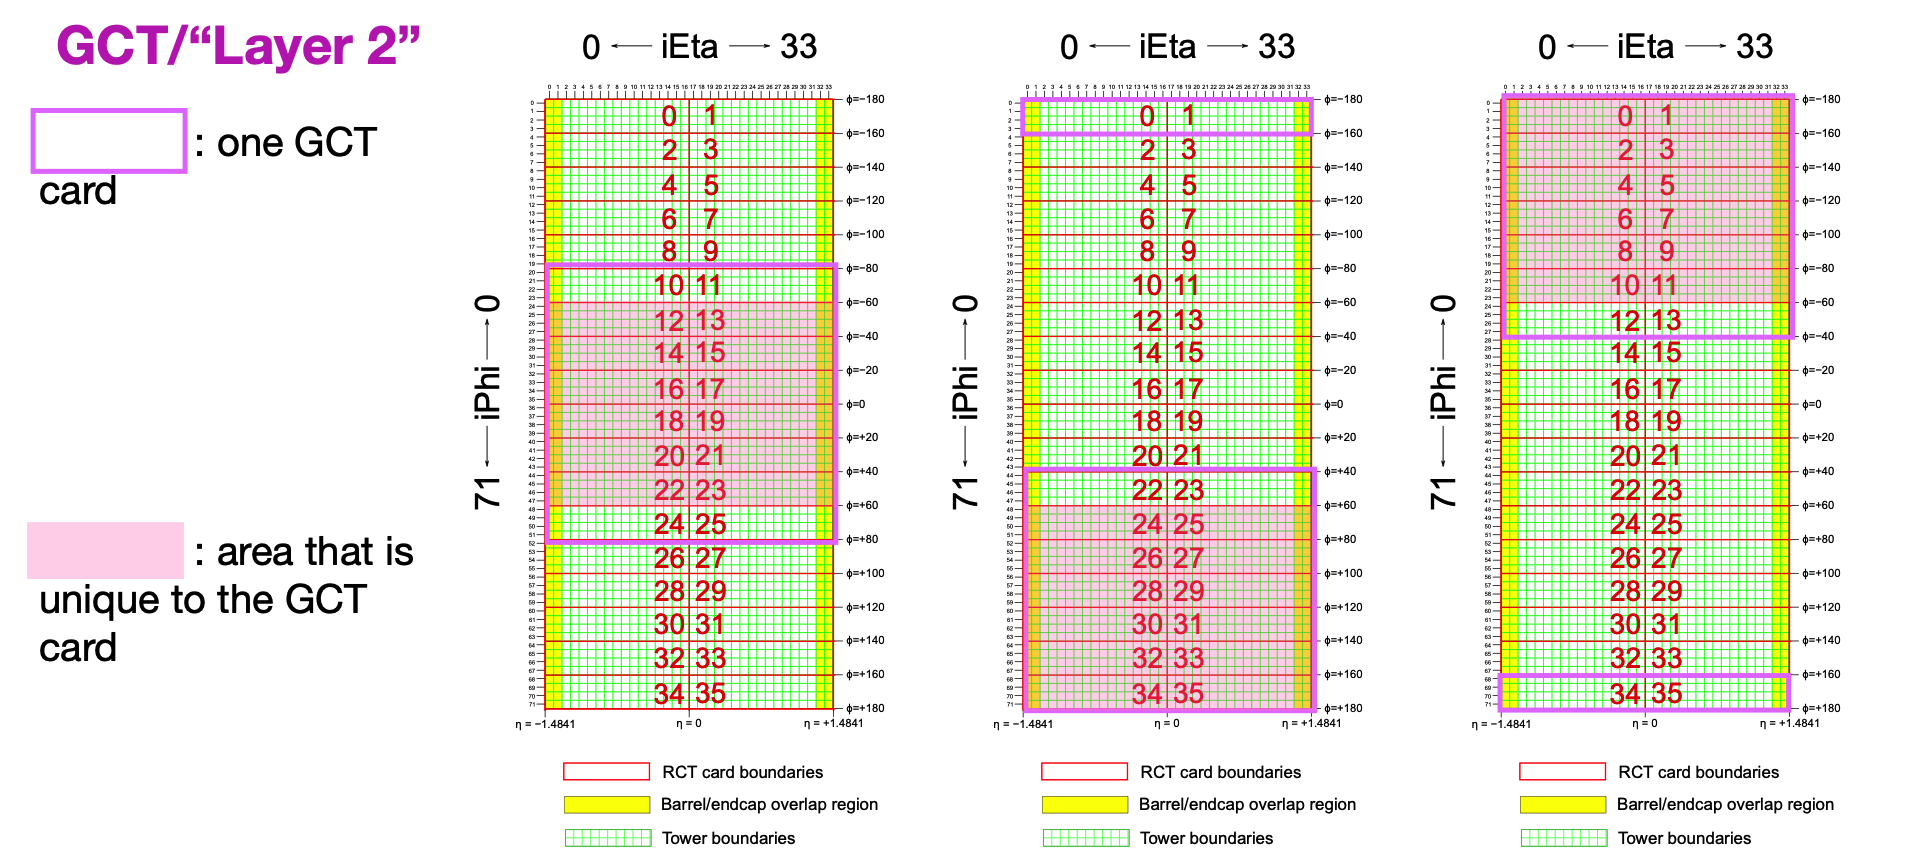
\includegraphics[width=15cm]{figures/ch-3-phase2/phase-2-gct-cards-schematic.png}
    \caption{Schematic of the Phase-2 ECAL barrel in the Global Calorimeter Trigger (GCT), which will process the outputs of the Regional Calorimeter Trigger (RCT) in three GCT cards (\textit{purple borders}). Each card in the GCT processes the equivalent of sixteen RCT cards, with the center twelve RCT cards being unique to that GCT card (\textit{shaded pink}), and the remaining four RCT cards overlapping with one other GCT card.}
    \label{fig:phase-2-gct-cards-schematic}
\end{figure}

The standalone barrel algorithm for reconstructing and identifying electrons and photons in the Phase-2 Level-1 Trigger takes as input the digitized response of each crystal of the barrel ECAL, with a granularity $0.0175 \times 0.0175$ in $\eta \times \phi$, which is 25 times higher than the input to the Phase-1 trigger, which consisted of trigger towers with a granularity of $0.0875 \times 0.0875$. In HCAL the tower size of $0.0875 \times 0.0875$ is unchanged. The trigger algorithm is designed to closely reproduce the algorithm used in the offline reconstruction, with limitations and simplifications due to trigger latency. 

\begin{figure}[ht]
    \centering
    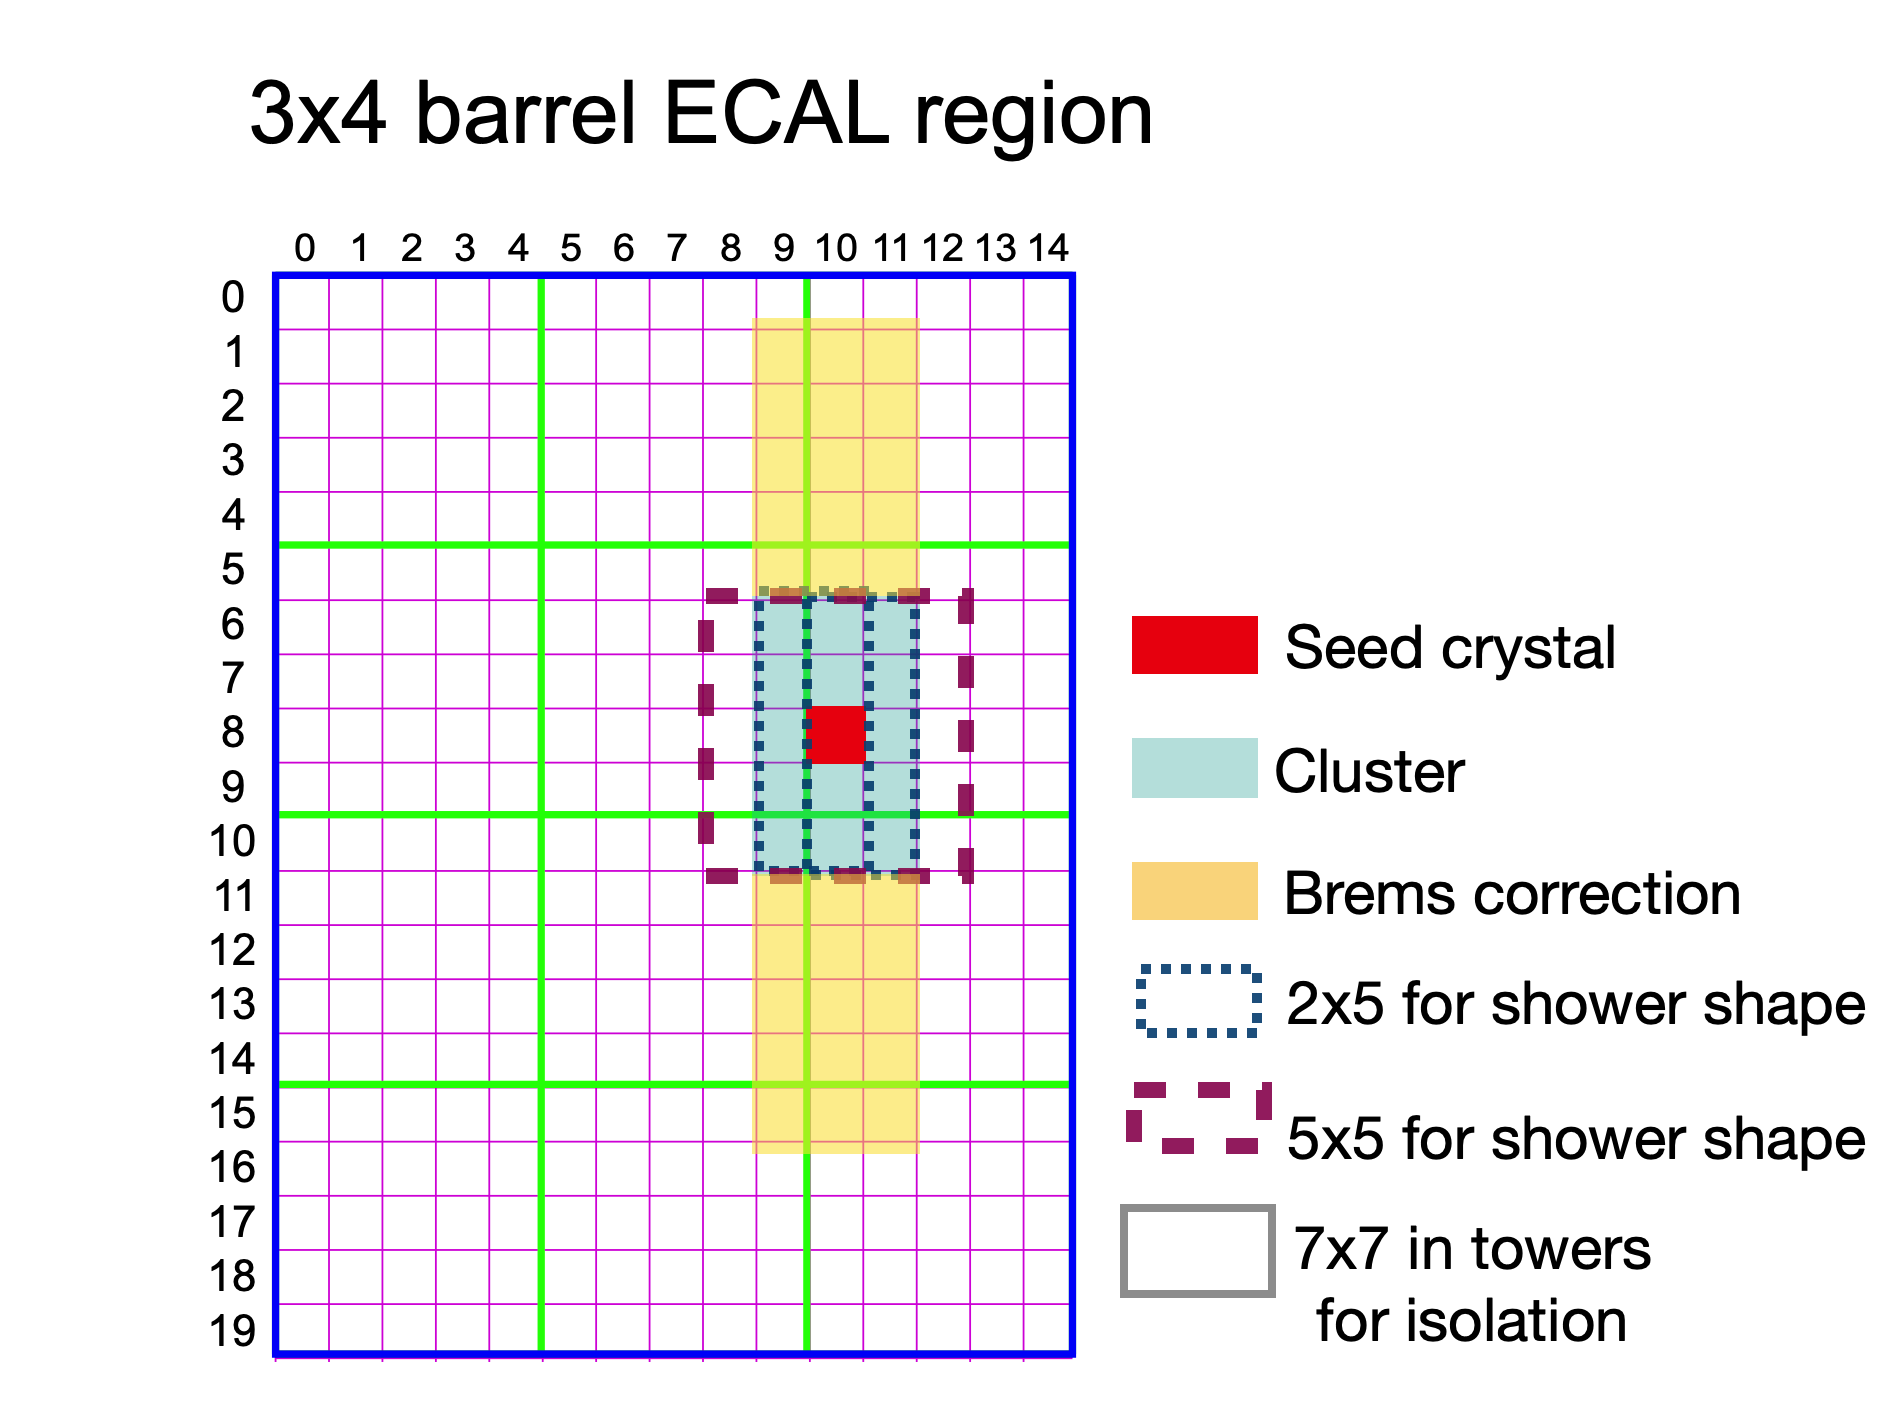
\includegraphics[width=12cm]{figures/ch-3-phase2/phase-2-cluster-footprint.png}
    \caption{Illustration of an example electron/photon ($e/\gamma$) cluster in the Phase-2 Level-1 Trigger standalone barrel $e/\gamma$ reconstruction, in a region of $15\times 20$ crystals ($3\times 4$ towers) in $\eta \times \phi$. Each small pink square is one crystal, the highest-granularity ECAL trigger primitives available to the L1 Trigger in Phase-2. The core cluster consists of the energy sum in a $3\times 5$ window of crystals (\textit{shaded light blue}), centered around the seed crystal (\textit{red}). The presence of energy lost to bremsstrahlung radiation is checked in the adjacent $3\times 5$ windows in the $\phi$ direction (\textit{shaded light yellow}). The ratio of the total energies in windows of size $2\times 5$ and $5\times 5$ in crystals (\textit{dashed dark blue and dark red}) around the seed crystal, is computed and compared to the core cluster energy to obtain shower shape flags. Lastly, the isolation, defined as the sum of the energy in a large window of size $7\times 7$ in towers (not shown in figure) is computed, and compared to the core cluster energy to obtain isolation flags.}
    \label{fig:phase-2-cluster-footprint}
\end{figure}


In the RCT, an initial requirement of $p_{T} > 0.5$ GeV is imposed on the input trigger primitives (i.e. energies from the ECAL crystals and HCAL towers) to reject contribution from pile-up. In one of the regions inside a RCT card (Fig. \ref{fig:phase-2-one-rct-card-schematic-landscape}), the crystal containing the highest energy deposit is identified as the seed crystal, as shown in Fig. \ref{fig:phase-2-cluster-footprint}. The energy in the crystals in a window of size $3\times 5$ in $\eta\times\phi$ around the seed cluster is added into a cluster. The energy is considered ``clustered''. The process is repeated with the remaining ``unclustered" energy, until up to four clusters are produced in the region. 

To improve $e/\gamma$ identification and to reduce background contributions, identification and reconstruction algorithms are implemented at this stage:
\begin{itemize}
    \item Shower shape: The energy deposit sums around the seed crystal is computed in windows of size $2 \times 5$ and $5 \times 5$ (Fig. \ref{fig:phase-2-cluster-footprint}, \textit{dashed lines}), with true $e/\gamma$ clusters tending to produce showers that deposit most of their energy in a $2 \times 5$ region. 
    \item Bremsstrahlung recovery: $e/\gamma$ tend to spread in the $\phi$ direction due to charged particles being bent by the magnetic field of the CMS solenoid. If sufficient energy comparable to the core $3 \times 5$ cluster is found in the adjacent $3 \times 5$ windows (Fig. \ref{fig:phase-2-cluster-footprint}, \textit{shaded yellow}), the energy is added to the core cluster and no longer considered unclustered energy.
\end{itemize}

After parallel processing in the regions, the clusters in a RCT card are stitched together if they are located directly along the borders of a region (Fig. \ref{fig:phase-2-rct-cards-schematic}). The remaining unclustered ECAL energy is summed into ECAL towers. 

From each RCT card, the twelve highest-energy clusters, as well as any remaining unclustered energy, are sent to the GCT. Since each GCT card has information from sixteen RCT cards (Fig. \ref{fig:phase-2-gct-cards-schematic}), final stitching across the boundaries of the RCT cards is performed. One more identification algorithm is performed at this stage:
\begin{itemize}
    \item Isolation: One handle to reject backgrounds from e.g. pile-up, comes from the tendency for background to be spread more uniformly across a large area in the detector, whereas genuine $e/\gamma$ are expected to produce showers concentrated in the $3 \times 5$ crystal window. The energy sum in a large window of $7 \times 7$ in towers is computed and used to reject background.
\end{itemize}
Flags that provide discrimination power between genuine $e/\gamma$ and background, are computed using the relative isolation and shower shape quantities. The standalone working point (WP) is defined as the logical OR of the relative isolation and shower shape flags. 

\subsection{Electron/photon standalone barrel output and results}
The performance of the current emulator of the standalone barrel $e/\gamma$ algorithm in Phase-2 conditions is quantified in efficiencies and rates. Efficiency is the fraction of true electrons that the algorithm can reconstruct and identify, and is evaluated in a Monte Carlo simulated sample containing electrons with transverse momentum $p_{T}$ ranging from 1 to 100\GeV.  The efficiencies of the current and previous emulaors as a function of the electron generator-level $p_{T}$ are shown in Fig. \ref{fig:results-egamma-efficiency-gt25}. 

The rates are the event rates that this reconstruction and identification algorithm would obtain if it were deployed in a trigger, assuming that proton-proton collisions are occurring at the 40 MHz event rate of the HL-LHC. The rate is reported as a function of the minimum energy threshold required by the trigger, and is estimated using a simulated sample of minimum bias events, i.e. generic proton-proton collisions without any specific physics selections. The rates for the current and previous emulator are shown in Fig. \ref{fig:results-egamma-rates}. 

\begin{figure}[ht]
    \centering
    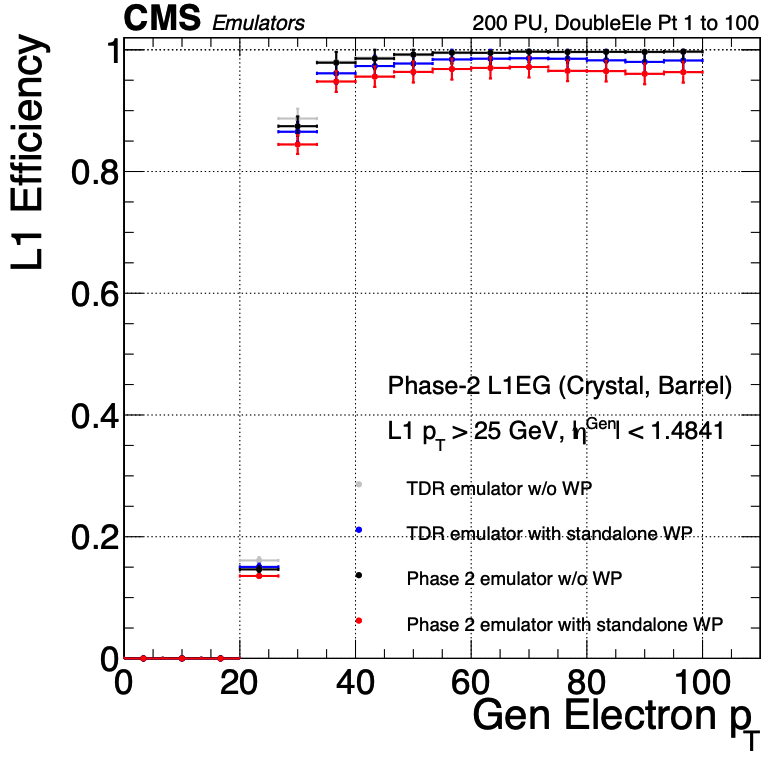
\includegraphics[width=12cm]{figures/ch-3-phase2/results-egamma-efficiency-gt25.png}
    \caption{Efficiencies of the current and previous emulators of the standalone barrel $e/\gamma$ algorithm for the Phase-2 Level-1 Trigger, evaluated in a simulated sample containing electrons, as a function of the electron's generator-level transverse momentum $p_{T}$. The standalone working point (WP) is defined as the logical OR of the isolation flag and shower shape flag. The efficiencies with and without requiring the standalone WP, are shown for the current emulator (labeled ``Phase 2", \textit{black, red}) and the previous emulator (labeled ``TDR", \textit{dark blue, grey}).}
    \label{fig:results-egamma-efficiency-gt25}
\end{figure}

\begin{figure}[h]
    \centering
    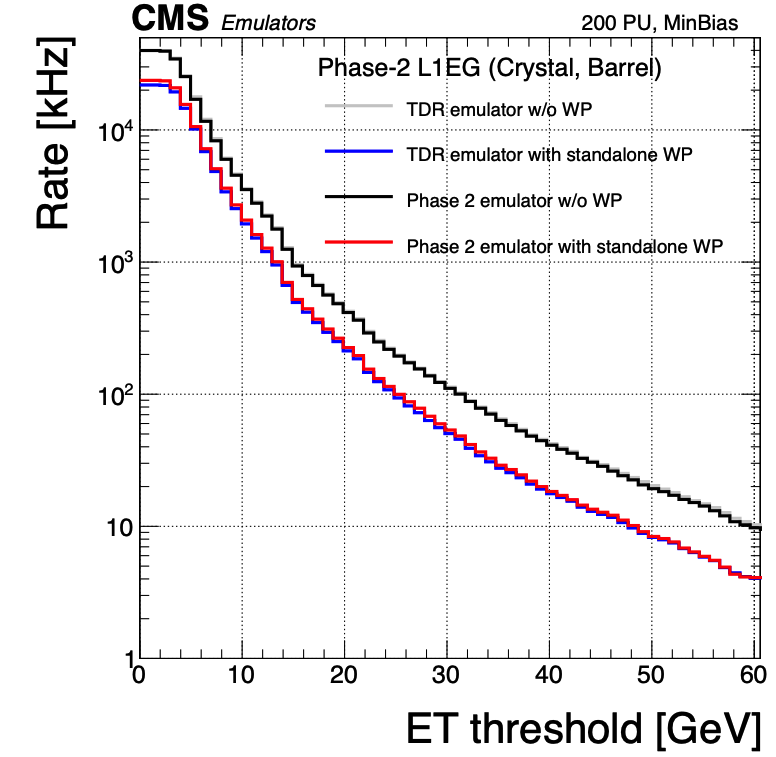
\includegraphics[width=12cm]{figures/ch-3-phase2/results-egamma-rates.png}
    \caption{Rates in kHz of the current Phase-2 and previous (``TDR") emulators of the standalone barrel $e/\gamma$ algorithm for the Phase-2 Level-1 Trigger, evaluated on a minimum bias (MinBias) sample with 200 pile-up (PU), measured as a function of the minimum energy ($E_T$) required of the reconstructed $e/\gamma$ object in each event. The standalone working point (standalone WP) is defined to be the logical OR of the isolation flag and the shower shape flag. The rates with and without requiring the standalone WP, are shown for the current emulator (labeled ``Phase 2", \textit{black, red}) and the previous emulator (labeled ``TDR", \textit{dark blue, grey}).}
    \label{fig:results-egamma-rates}
\end{figure}

% TODO: discuss performance in menu

The information of the clusters in the event, including their energies, crystal-level position, the relative isolation flag, the shower shape flag, the standalone WP, and the ratio of the HCAL over ECAL energies, are sent in digitized ``words" of 64 bits to the Correlator Trigger and the Global Trigger. The towers in the event are computed as the sum of all unclustered energy in the ECAL with the corresponding HCAL energy at each tower location, and their energies are sent to the Correlator Trigger.

% TODO: talk about how the outputs are used

\chapter{Datasets and Monte Carlo samples}
\section{Datasets used}
The $h \rightarrow aa \rightarrow 2b2\tau$ analysis (CMS CADI line HIG-22-007) is based on proton-proton collision data at a center-of-mass energy of 13 TeV collected in full Run-2 (2016-18) with the CMS detector. The data analyzed corresponds to a total integrated luminosity of 138 fb$^{-1}$ (36.33 fb$^{-1}$ for 2016, 41.53 fb$^{-1}$ for 2017, and 59.74 fb$^{-1}$ for 2018) \cite{CMS-LUM-17-001} \cite{CMS-LUM-17-004} \cite{CMS-LUM-18-002}. 

Data collected with the single muon trigger is used for the $\mu\tau_{h}$ channel. For the $e\tau_{h}$ channel, data collected with the single electron trigger is used; and for the $e\mu$ channel, data collected with the electron $+$ muon trigger is used. A more in-depth discussion of the triggers used follows in a later section.

A full list of samples used can be found in the full documentation \cite{CMS-HIG-22-007} \cite{CMS-PAS-HIG-22-007}.

\section{Monte Carlo samples}
Modeling and computing observables originating from arbitrary physics processes at the tree level and at next-to-leading order (NLO) is performed by Monte Carlo (MC) event generators, such as Powheg and MadGraph5\_amC\@NLO \cite{Alwall_2014} \cite{Frederix_2018}. The information generated, e.g. the computation of the differential cross sections and kinematics of the final state particles, is saved in a compressed file and used to generate MC samples that are used in physics analyses. The samples are digitized using GEANT4 \cite{agostinelli_geant4simulation_2003}, a platform used at the LHC and other facilities to comprehensively simulate the passage of particles through matter. The digitized samples are passed through the same detector reconstruction as real data events collected in the detector.

The samples for modeling the signal ($h \rightarrow aa \rightarrow 2b2\tau$ and $h\rightarrow a_1 a_2$) in the 2HDM+S and TRSM are generated at tree-level, for a range of masses of the light neutral scalar $a$. For $h \rightarrow aa$, the mass hypotheses for the $a$ range from $m_a = (12 \,\text{GeV}, 62.5 \,\text{GeV})$. For $h \rightarrow a_1 a_2$, the mass hypotheses for the two light scalars span combinations of $m_{a1}$, $m_{a2}$ ranging from $(12 \,\text{GeV}, 62.5 \,\text{GeV})$ for the two scalars.


\section{Embedded samples}
\label{sec:embedded-samples}
An embedding technique is used to estimate background from the Standard Model $Z$ boson decaying to $\tau\tau$, from data with minimal simulation input \cite{CMS-TAU-18-001}. In data events selected to have $Z \rightarrow \mu\mu$ decays, all energy deposits of the recorded muons are removed from the event, and replaced with simulated tau leptons with the same kinematic properties as the removed muons. This results in a hybrid data format containing information from both observed and simulated events. The advantage of the Embedded samples is that the portions of the event that are difficult to model and describe (e.g. the underlying event or production of additional jets) are directly taken from data. 


\chapter{Object reconstruction and corrections applied}
\section{Object reconstruction}

We review the properties of the particles most pertinent to the analyses presented in this work (taus, muons, electrons, jets, and b-jets), their signatures in the CMS detector, and dedicated reconstruction techniques used at CMS.

\subsection{Taus}
The tau ($\tau$) is the heaviest known lepton. With a rest mass of 1776.86 MeV, it can decay to not only electrons and muons, but also hadrons. The mean lifetime of the $\tau$ is $\tau = 290 \times 10^{-15}$ seconds, corresponding to $c\tau = 87.03$ $\mu$m, which is short enough that taus decay in the CMS detector before reaching the detector elements. 

In two thirds of the cases, $\tau$ leptons decay hadronically, typically into one or three charged mesons (predominantly $\pi^+$, $\pi^-$), often accompanied by neutral pions (that decay $\pi^0 \rightarrow \gamma\gamma$), and a $\nu_{\tau}$. These hadronic decays are denoted $\tau_{h}$. In the remainder of the decays, the tau decays to the lighter leptons (electron or muon), termed leptonic decays. In all cases, at least one neutrino is produced, resulting in missing transverse energy in the CMS detector. The tau's largest decay branching ratios (proportional to probability of decay) are listed below \citep{workman_review_2022}: 
\begin{itemize}
    \item 17.8\% decay to $e^- \bar{\nu}_e \nu_{\tau}$
    \item 17.4\% decay to $\mu^- \bar{\nu}_\mu \nu_{\tau}$
    \item 25.5\% decay to $\pi^- \pi^0 \nu_{\tau}$ ($\rho^-$ resonance at 770 MeV)
    \item 10.8\% decay to $\pi^- \nu_{\tau}$ % (excluding $K^0, \omega$)
    \item 9.3\% decay to $\pi^- \pi^0 \pi^0 \nu_{\tau}$  ($a_1^-$ resonance at 1200 MeV)
    \item 9.0\% decay to $\pi^- \pi^- \pi^+ \nu_{\tau}$ ($a_1^-$ resonance at 1200 MeV)
\end{itemize}

The neutrinos escape undetected from the CMS detector and are not considered in the reconstruction. Charged hadrons leave tracks in the tracking detector before being absorbed in the hadronic calorimeter; in CMS tau reconstruction terminology, they are often called ``prongs'', i.e. the dominant $\tau_{h}$ decay modes are termed ``1 prong" ($\pi^\pm$), ``1 prong + $\pi^0$(s)", and ``3-prong''. Neutral pions decay to two photons which lose their energy in the electromagnetic calorimeter. Taus that decay to electrons and muons, are typically triggered on and reconstructed as electrons and muons respectively. 

\subsubsection{Hadron plus strips (HPS) reconstruction of \texorpdfstring{$\tau_{h}$}{tauh}}
At CMS, hadronically decaying tau leptons are reconstructed with the hadron plus strips (HPS) algorithm \citep{CMS-TAU-14-001} \cite{2012-JINST-7-P01001}. The HPS algorithm capitalizes on photon conversions in the CMS tracker material, which originate from the neutral pion ($\pi^0$) decaying to two photons. The bending of electron/positron tracks due to the CMS solenoid magnetic field leads to a spread of the neutral pions' calorimeter signatures in the $\phi$ direction. This motivates the reconstruction of photons in ``strips": objects that are built out of PF photons and electrons. The strip reconstruction starts with centering a strip on the most energetic electromagnetic particle in a PF jet. Among other electromagnetic particles located in a window of size $\Delta \eta = 0.05$ and $\Delta \phi = 0.20$ around the strip center, the most energetic one is associated with the strip and its momentum is added to the strip momentum. This is repeated iteratively until no further particles can be associated. Lastly, strips satisfying a requirement of $p_{T}^{\text{strip}} > 1$ GeV are combined with charged hadrons to reconstruct individual $\tau_{h}$ decay modes, where $h$ stands for both $\pi$ and $K$:
\begin{itemize}
    \item \textit{Single hadron}: $h^- \nu_{\tau}$ and $h^- \pi^0 \nu_{\tau}$ decay modes, in which the neutral pions have too little energy to be reconstructed as strips.
    \item \textit{One hadron + one strip}: $h^- \pi^0 \nu_{\tau}$ decay modes, where the photons from the $\pi^0$ decay are close together in the calorimeter.
    \item \textit{One hadron + two strips}: $h^- \pi^0 \nu_{\tau}$ decay modes, where the photons from the $\pi^0$ decay are well separated. 
    \item \textit{Three hadrons}: $h^- h^+ h^- \nu_{\tau}$ decay modes. The three charged hadrons are required to originate from the same secondary vertex.
\end{itemize}
The $h^- \pi^0 \pi^0 \nu_{\tau}$ and $h^- h^+ h^- \pi^0 \nu_{\tau}$ decay modes do not have their own treatment are reconstructed with the above topologies. 

In the HPS algorithm, the direction of the reconstructed tau momentum $\vec{p}^{\tau_{h}}$ is required to fall within a distance of $\Delta R = 0.1$ from the original PF jet. All charged hadrons and strips are required to be contained within a cone of size $\Delta R = (2.8 \,\text{GeV})/p_{T}^{\tau_{h}}$, from the $\tau_{h}$ as reconstructed by the HPS. 

All charged hadrons are assumed to be pions, and they are required to be consistent with the masses of the intermediate meson resonances (if applicable), with the following allowed windows for candidates: 50-200 MeV for $\pi^0$, 0.3-1.3 GeV for $\rho$, and 0.8-1.5 GeV for $a_1$. If the $\tau_{h}$ decay is compatible with more than one hypothesis, the one giving the highest $p_{T}^{\tau_{h}}$ is chosen. Lastly, an isolation requirement is applied: aside from the $\tau_{h}$ decay products, no charged hadrons or photons can be present within an isolation cone of size $\Delta R = 0.5$ around the direction of the $\tau_{h}$. The outputs of the HPS algorithm are the reconstructed decay mode and the visible four-momentum (i.e. the four-momenta of all decay products excluding the neutrinos).

\subsubsection{DeepTau for identifying \texorpdfstring{$\tau_{h}$}{tauh}}
The identification of $\tau_{h}$ candidates in CMS has historically been divided into separate discriminators against jets, electrons, and muons. Discriminators versus jets and electrons use information from derived quantities, such as the $p_{T}$ sum of particles near the $\tau_{h}$ axis. Building on the previous multivariate analysis (MVA) classifier \cite{CMS-TAU-16-003} based on a boosted decision tree (BDT), DeepTau is a more recent classifier based on a deep neural network (DNN) that simultaneously discriminates against jets, electrons, and muons. The DNN uses a combination of high-level inputs, similar to previous algorithms, and also uses convolutional layers in $\eta$-$\phi$ space to process information from all reconstructed particles near the $\tau_{h}$ axis. Convolutional layers are based on the principle that an image can be processed independently of its position. 

The final DeepTau discriminators against jets, muons, and electrons are given by 
\begin{equation}
    D_\alpha(y) = \frac{y_{\tau}}{y_{\tau} + y_{\alpha}}
\end{equation}
where $y_\tau$ ($y_\alpha$) are estimates of the probabilities for the $\tau_{h}$ candidate to come from a genuine $\tau_{h}$ (jet, $\mu$, $e$). Working points for each discriminator with different $\tau_{h}$ identification efficiencies are defined for $D_{e}$, $D_{\mu}$, and $D_{\text{jet}}$, for usage in physics analyses and derivation of data-to-simulation corrections \cite{2022-PRD-DeepTau}. 

\subsection{Muons}
\label{section:ch-5-muon-reconstruction}
Muons are the next lightest lepton after taus, with a mass of $105.66$ MeV and a mean lifetime of $\tau = 2.20 \times 10^{-6}$ seconds, or $c\tau = 658.64$ m. At CMS, muons are identified with requirements on the quality of the track reconstruction and on the number of measurements in the tracker and the muon systems \citep{CMS-MUO-10-004}. In the standard CMS reconstruction, tracks are first reconstructed independently in the inner tracker (tracker track) and in the muon system (standalone-muon track). Next, these tracks are processed in two different methods.

The first is Global Muon reconstruction (outside-in) \citep{CMS-MUO-10-004}, which fits combined hits from the tracker track and standalone-muon track, using the Kalman-filter technique. At large transverse momenta, $p_{T} \gtrsim 200$ GeV, the global-muon fit can improve the momentum resolution compared to the tracker-only fit. 

The second is Tracker Muon reconstruction (inside-out) \citep{CMS-MUO-10-004}, which starts with tracker tracks with $p_{T} > 0.5$ GeV and total momentum $p_{T} > 2.5$ GeV. These tracks are extrapolated outwards to the muon system and matched to detector segments there, taking into account the magnetic field, expected energy losses, and multiple Coulomb scattering in the detector material. Tracker Muon reconstruction is more efficient than the Global Muon reconstruction at low momenta, $p \lesssim 5$ GeV, because it only requires a single muon segment in the muon system, where as Global Muon reconstruction typically requires segments in at least two muon stations.

To further suppress fake muons from decay in flight, isolation cuts are used. A relative isolation variable is defined to quantify the energy flow of particles near the muon trajectory.
A relative isolation is defined similarly for muons and electrons:
\begin{equation}
    I^\ell \equiv \frac{\sum_{\text{charged}} p_{T} + \text{max}\left( 0, \sum_{\text{neutral}} p_{T} - \frac{1}{2}  \sum_{\text{charged, PU}} p_{T}  \right)}{p_{T}^\ell}
    \label{eqn:definition-relative-isolation}
\end{equation}
where $\sum_{\text{charged}} p_{T}$ is the scalar sum of the $p_{T}$ of the charged particles originating from the primary vertex and located in a cone of size $\Delta R = \sqrt{(\Delta \eta)^2 + (\Delta \phi)^2} = 0.4 (0.3)$ centered on the direction of the muon (electron). The sum $\sum_{\text{neutral}} p_{T}$ is the equivalent for neutral particles. The sum $\sum_{\text{charged, PU}} p_{T}$ is the scalar sum of the $p_{T}$ of the charged hadrons in the cone originating from pileup vertices. The factor $1/2$ comes from simulation estimations, which find that the ratio of neutral to charged hadron production in the hadronization process of inelastic $pp$ collisions is $1/2$. Thus the subtracted term is intended to subtract contribution from pileup, from the neutral particle contribution to the isolation sum. Finally, this is divided by the lepton transverse momentum, $p_{T}^\ell$. 


\subsection{Electrons}
Electrons are the lighest lepton with a mass of $0.511$ MeV. At CMS, electrons are reconstructed by associating a track reconstructed in the silicon tracking detector with a cluster of energy in the ECAL. Performance is maximized via a combination of a stand-alone approach and the complementary global particle-flow approach \citep{JINST-2015-10-P06005}. 

In the stand-alone approach, the electron energy, which is typically spread over several crystals of the ECAL, is clustered with the ``hybrid'' algorithm in the barrel and the ``multi-$5\times 5$'' in the endcaps \citep{JINST-2015-10-P06005}. The hybrid algorithm collects energy in a small window in $\eta$ and an extended window in $\phi$. It identifies a seed crystal, and adds arrays of $5 \times 1$ crystals in $\eta \times \phi$ in a range of $N = 17$ crystals in both directions of $\phi$, if their energies exceed a minimum threshold, thus forming a supercluster (SC).  In the endcap, crystals are not arranged in an $\eta \times \phi$ geometry; instead clusters are build around seed crystals in clusters of $5\times 5$ crystals that can partly overlap. Nearby clusters are grouped into a supercluster, and energy is recovered from associated deposits in the preshower. 

In the PF reconstruction \citep{JINST-2015-10-P06005}, PF clusters are reconstructed by aggregating around a seed all contiguous crystals with energies two standard deviations above the electronic noise observed at the beginning of a data-taking run. The energy of a given crystal can be shared among two or more clusters.

The electron track reconstruction is performed in two ways \citep{JINST-2015-10-P06005}: the ECAL-based seeding, which begins with the SC energy and positioning, and the tracker-based seeding (part of the PF reconstruction algorithm), which uses tracks reconstructed from the general algorithm for charged particles, extrapolated towards the ECAL and matched to an SC. Kalman filter (KF) tracks with a small number of hits or that are not well-fitted, are re-fitted with a dedicated Gaussian sum Filter (GSF).

A global identification variable \citep{JINST-2015-10-P06005} is defined using a multivariate analysis (MVA) technique that combines information on track observables (kinematics, quality of the KF track and GSF track), the electron PF cluster observables (shape and pattern), and the association between the two (geometric and kinematic observables). For electrons seeded only through the tracker-based approach, a weak selection is applied on this MVA variable. For electrons seeded through both approaches, a logical OR is taken. 

Electron isolation, i.e. the presence of energy deposits near the electron trajectory, is a separate key handle in rejecting significant background. Compared to isolated electrons, electrons from misidentified jets or genuine electrons within a jet resulting from semileptonic decays of $b$ or $c$ quarks tend to have significant energy deposits near the primary trajectory \citep{JINST-2015-10-P06005}. Offline analyses benefit from the PF technique for defining isolation, which sums the PF candidates reconstructed located within a specified isolation cone around the electron candidate, as in Eqn. \ref{eqn:definition-relative-isolation}.

\subsection{Jets}
The vast majority of processes of interest at the LHC contains quarks or gluons in the final state, but these particles cannot be observed directly. In a process called hadronization, they fragment into spatially-grouped collections of particles called jets, which can be detected in the tracking and calorimeter systems. Hadronization and the subsequent decays of unstable hadrons can produce hundreds of nearby particles in the CMS detector. Jets are reconstructed by the PF algorithm (PF jets), or from the sum of the ECAL and HCAL energies deposited in the calorimeter towers (Calo jets). In PF jets, typically used in offline analyses, jets are built using the anti-$k_T$ (AK) clustering algorithm \cite{CMS-BTV-12-001}. The anti-$k_T$ algorithm iterates over particle pairs and finds the two that are closest in a distance measure $d$, and determines whether to combine them:
\begin{equation}
    d_{ij} = \text{min} \left(p_{T, i}^{-2}, \, p_{T, j}^{-2} \right) \frac{\Delta_{ij}^2}{R^2}, \, \,
    \text{combine when $d_{ij} < p_{T,i}^{-2}$; stop when $d_{ij} > p_{T, i}^{-2}$}
    \label{eqn:anti-kT}
\end{equation}
where $\Delta_{ij}^2 = (\eta_i - \eta_j)^2 + (\phi_i - \phi_j)^2$ and $p_{T, i}$, $\eta_i$, $\phi_i$ are the transverse momentum, rapidity, and azimuthal angle of particle $i$. The power $-2$ means that higher-momentum particles are clustered first, leading to jets that tend to be centered on the hardest (highest $p_T$) particle.

There are several methods to remove contributions of pileup collisions from jet clustering \cite{CMS-PAS-JME-14-001}:
\begin{itemize}
    \item Charged hadron subtraction (CHS), which removes all charged hadron candidates associated with a track that is not associated with the primary vertex.
    \item PileUp Per Particle Identification (PUPPI), which weighs input particles based on their likelihood of arising from pileup. QCD particles tend to have a collinear structure, compared to soft diffuse radiation coming from pileup. The local shape for charged pileup, used as a proxy for all pileup particles, is used on an event-by-event basis to calculate a weight for each particle. PUPPI is deployed in Run-2 and is more performant than CHS in high pileup scenarios.
\end{itemize}

\subsection{B jets}
Jets that arise from bottom-quark hadronization (b jets) have overwhelming background from processes involving jets from gluons (g) and light-flavour quarks (u, d, s), and from c-quark fragmentation. The ability to identify b jets, or b-tagging, exploits the b hadrons' relatively large masses, long lifetimes, and daughter particles with hard momentum spectra \cite{CMS-BTV-12-001}. 

The impact parameter (IP) of a track is the 3-dimensional distance between the track and the primary vertex (PV) at the point of closest approach. The IP is positive if the track originates from the decay of particles travelling along the jet axis. The resolution of the IP depends on the $p_{T}$ and $\eta$ of the track, motivating the use of the impact parameter significance $S_{\text{IP}}$ (ratio of the IP to its estimated uncertainty) as an observable \cite{CMS-BTV-12-001}.

Because of the large but finite lifetimes of the b hadrons, b hadrons tend to travel a short distance before decaying at a secondary vertex (SV), which can be measured and reconstructed separately from the primary vertex due to the excellent position resolution of the pixel detector \cite{CMS-BTV-12-001}. Previous b-tagging algorithms (e.g. CSV, cMVAv2, and DeepCSV) have capitalized on variables such as the presence of a SV, the flight distance and direction (computed from the vector between the PV and the SV), and kinematics of the system of associated secondary tracks (e.g. track multiplicity, mass, and energy). 

The DeepJet (formerly known as DeepFlavour) algorithm \cite{CMS-DP-2017-013} is a deep-neural-network multi-classification algorithm, which uses 16 properties of up to 25 charged and 6 properties of 25 neutral particle-flow jet constituents, as well as 17 properties from up to 4 secondary vertices associate with the jet. Compared to the previous classifying algorithm DeepCSV, DeepJet has been demonstrated to have higher efficiency with lower misidentification probability in Phase-1 data \cite{CMS-DP-2018-058}. 



\section{Reconstruction of the \texorpdfstring{$\tau\tau$}{tautau} mass}

The final signal extraction is done to the total $\tau\tau$ mass, which is estimated from the visible $\tau\tau$ mass using the FastMTT algorithm \cite{2014_SVFit_Bianchini}. FastMTT is based on the SVFit algorithm, originally developed for the Standard Model $H \rightarrow \tau\tau$ analysis \cite{CMS-HIG-13-004}. Both the SVFit algorithms, and the FastMTT algorithm, are described below, to give a complete picture of how tau decays are parameterized.

To specify a hadronic $\tau$ decay, six parameters are needed \cite{CMS-HIG-13-004}: the polar and azimuthal angles of the visible decay product system in the $\tau$ rest frame, the three boost parameters from the $\tau$ rest frame to the laboratory frame, and the invariant mass $m_{\text{vis}}$ of the visible decay products. For a leptonic $\tau$ decay, two neutrinos are produced, and a seventh parameter, the invariant mass of the two-neutrino system, is necessary. The unknown parameters are constrained by four observables that are the components of the four-momentum of the system formed by the visible decay products of the $\tau$ lepton, measured in the laboratory frame. The remaining unconstrained parameters for hadronic and leptonic $\tau$ decays are thus:

\begin{itemize}
    \item The fraction of the $\tau$ energy in the laboratory frame carried by the visible decay products,
    \item $\phi$, the azimuthal angle of the $\tau$ direction in the laboratory frame,
    \item $m_\nu\nu$, the invariant mass of the two-neutrino system in leptonic $\tau$ decays (for hadronic $\tau$ decays, $m_{\nu\nu}$ is set to 0).
\end{itemize}
$E_{x}^{\text{miss}}$ and $E_{y}^{\text{miss}}$, the $x$ and $y$ components of the missing transverse energy $E_{T}^{\text{miss}}$ provide two further constraints. 

\subsection{Original SVFit \texorpdfstring{``standalone"}{"standalone"}: maximum likelihood}
In one of the original versions of SVFit, called ``standalone'' SVFit \cite{CMS-HIG-13-004}, a maximum likelihood fit method is used to reconstruct the mass $m_{\tau\tau}$ by combining the measured observables $E_{x}^{\text{miss}}$ and $E_{y}^{\text{miss}}$ with a likelihood model that includes terms for the $\tau$ decay kinematics and the $E_{T}^{\text{miss}}$ resolution \cite{CMS-HIG-13-004}. The likelihood function $f(\vec{z}, \vec{y}, \vec{a}_1 \vec{a}_2)$ of the parameters $\vec{z} = (E_{x}^{\text{miss}}, E_{y}^{\text{miss}})$ in an event is constructed, where the remaining parameters are the kinematics of the two $\tau$ decays, denoted $\vec{a}_1 = (x_1, \phi_1, m_{\nu\nu, 1})$ and $\vec{a}_2 = (x_2, \phi_2, m_{\nu\nu, 2})$, and the four-momenta of the visible decay products with the measured values $\vec{y} = (p_1^{\text{vis}}, p_2^{\text{vis}})$.

The likelihood $f$ is the product of three likelihood functions. The first two likelihood functions model the decay parameters $\vec{a}_1$ and $\vec{a}_2$ of the two $\tau$ leptons. For leptonic decays, the likelihood function is modeled using matrix elements for $\tau$ decays, and integrated over the allowed phase space $0 \leq x \leq 1$ and $0 \leq m_{\nu\nu} \leq m_{\tau} \sqrt{1-x}$. For hadronic $\tau$ decays, a model based on the two-body phase space is used and integrated over $m_{\text{vis}}^2/ m_{\tau\tau}^2 \leq x \leq 1$. The third likelihood function quantifies the compatibility of a $\tau$ decay hypothesis with the reconstructed $\vec{E}_{T}^{\text{miss}}$ in an event, assuming the neutrinos are the only source of missing transverse energy. The expected $\vec{E}_{T}^{\text{miss}}$ resolution is represented by a covariant matrix, estimated on an event-by-event basis using a significance algorithm \cite{CMS-JME-10-009}.

\subsection{\texorpdfstring{``Classic SVFit"}{"Classic SVFit} with matrix element}
Classic SVFit is an improved algorithm of the original ``standalone" SVFit using the formalism of the matrix element (ME) method \cite{2014_SVFit_Bianchini}. In the ME method, an estimate for the unknown model parameter $\Theta$ (here, the mass $m_{\tau\tau}$) is obtained by maximizing the probability density $\mathcal{P}$. The key ingredients of the probability density are the squared modulus of the matrix element $|\mathcal{M}(\mathbf{p}, \Theta)|^2$ and the transfer function $W(\mathbf{y}|\mathbf{p})$ (probability density to observe the measured observables $\mathbf{y}$ given the phase space point $\mathbf{p}$). The best estimate $m_{\tau\tau}$ is obtained by computing the probability density $\mathcal{P}$ for a range of mass hypotheses and finding the value of $m_{\tau\tau}$ that maximizes $\mathcal{P}$.

Distributions illustrating the performance of the classic matrix element SVFit algorithm are shown in Fig. \ref{fig:classic_svfit_resolution} from \cite{2014_SVFit_Bianchini}, showing the di-tau mass after and before application of SVFit to recover energy lost to neutrinos. The SVFit algorithm is found to improve the sensitivity of the Standard Model $H \rightarrow \tau\tau$ analysis performed by CMS by about 30\%, compared to performing the same analysis using only the visible mass $m_{\text{vis}}$. 

\begin{figure}[ht]
    \centering
    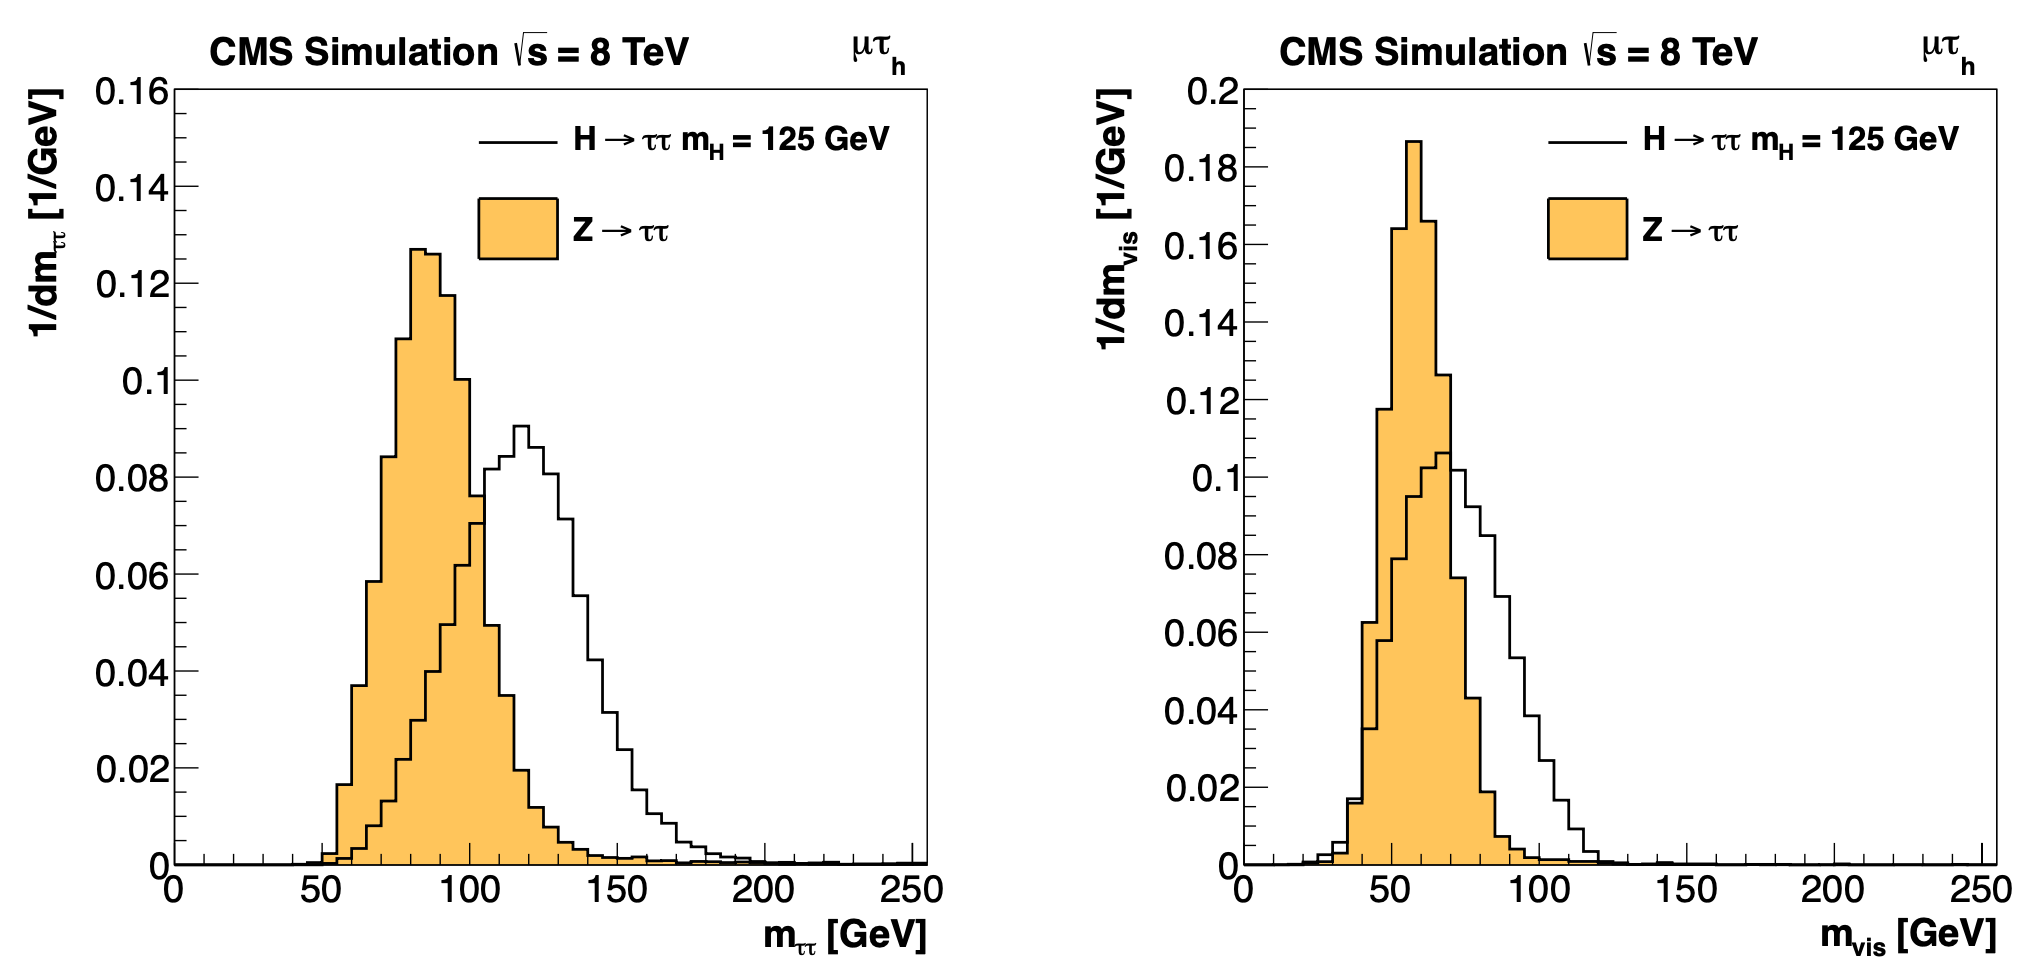
\includegraphics[width=15cm]{figures/ch-5-object-reconstruction-and-corrections-applied/original_SVFit_resolution_2014_SVFit_Bianchini.png}
    \caption[Distributions of $m_{\tau\tau}$ reconstructed by the classic SVFit algorithm, and masses of visible tau decay products (before SVFit).]{Distributions from \cite{2014_SVFit_Bianchini}, of $m_{\tau\tau}$ after reconstruction with the original SVFit algorithm (\textit{left}), and before SVFit with only the visible tau decay products (\textit{right}), for $H \rightarrow \tau\tau$ signal events of mass $m_H = 125$ GeV (\textit{black line}) and the $Z/\gamma^* \rightarrow \tau\tau$ background (\textit{orange, solid}), in the decay channel $\tau\tau \rightarrow \mu\tau_{h}$.} 
    \label{fig:classic_svfit_resolution}
\end{figure}


\subsection{FastMTT: optimized SVFit}
FastMTT \cite{CMS-AN-19-032-FastMTT} is a further simplification to the matrix element method of Classic SVFit which has comparable performance but is about 100 times faster. FastMTT drops the matrix element component of the computation without significant impact on the final mass resolution, and simplifies the computation of the transfer functions. The opening angle of the $\tau$ decay products with respect to the initial $\tau$ momenta approaches 0 for $\tau$ with high $\gamma = E_{\tau}/m_{\tau}$, with typical $\tau$ decays from the Z boson decays already satisfying this condition. In this collinear approximation, the dimensionality of the transfer function can be reduced in the computation of FastMTT, while still yielding similar results to Classic SVFit \cite{CMS-AN-19-032-FastMTT}. 

\section{Corrections applied to simulation}
\label{sec:corrections_applied}

Corrections are applied to simulated samples to account for known effects in the event modeling and reconstruction and data-taking, and are intended to bring simulations in closer agreement with data. Corrections fall into two broad categories: \textit{energy scale corrections} applied to physics objects, and \textit{event-level corrections}. Energy scale corrections are multiplicative factors applied to the energy and transverse momentum $p_{T}$ of simulated objects (e.g. leptons or jets), and bring the average reconstructed energies of simulated particles into better agreement with those of objects reconstructed from data. Event-level corrections are applied as a per-event multiplicative weight, and account for effects such as mis-modeling in simulations of the underlying physics process, or changing detector operating conditions during data-taking. Event-level corrections change the shapes of the distributions of all the physical observables.  

Uncertainties in scale factors and corrections are also sources of systematic errors in the analysis, detailed in Chapter \ref{chapter:ch-8:systematic-uncertainties}. Systematic uncertainties in the tau, muon, and electron energy scales can shift the $p_{T}$ of the leptons up or down, which can change whether events pass or fail the offline $p_{T}$ thresholds for the trigger paths described in the previous section, i.e. change the number of events in the signal region.  

\subsection{Tau energy scale}
\label{sec:tau_energy_scale}

An energy scale is applied to the transverse momentum $p_{T}$ and mass of the hadronic tau $\tau_{h}$ in the $\mu\tau_{h}$ and $e\tau_{h}$ channels, to correct for a deviation of the average reconstructed $\tau_{h}$ energy from the generator-level energy of the visible $\tau_{h}$ decay products. These correction factors are derived centrally \cite{CMS-TAU-16-003}, by fitting to events in $e\tau_{h}$ and $\mu\tau_{h}$ final states in $Z/\gamma^*$ events separately for the $h^\pm$, $h^\pm \pi^0$, and $h^\pm h^\mp h^\pm$ decays. The values used are shown in Table \ref{table:tau-ES}.

When applying the energy scale to the $\tau_{h}$, the 4-momentum of the missing transverse energy (MET) is adjusted such that the total 4-momenta of the $\tau_{h}$ and the MET remains unchanged \cite{twiki_TAU_POG_tauidrecommendationforrun2}.

\begin{table}[ht]
    \centering
    \begin{tabular}{|c|c|c|c|c|}
    \hline
    \multicolumn{5}{|c|}{Tau energy scale factor}                                   \\ \hline
    \hline
    Decay mode      & 2018              & 2017              & 2016 pre-VFP      & 2016 post-VFP     \\ \hline
    0               & 0.991 $\pm$ 0.008 & 0.986 $\pm$ 0.009 & 0.987 $\pm$ 0.01  & 0.993 $\pm$ 0.009 \\
    1               & 1.004 $\pm$ 0.006 & 0.999 $\pm$ 0.006 & 0.998 $\pm$ 0.006 & 0.991 $\pm$ 0.007 \\
    10              & 0.998 $\pm$ 0.007 & 0.999 $\pm$ 0.007 & 0.984 $\pm$ 0.008 & 1.001 $\pm$ 0.007 \\
    11              & 1.004 $\pm$ 0.009 & 0.996 $\pm$ 0.01  & 0.999 $\pm$ 0.011 & 0.997 $\pm$ 0.016 \\ \hline
    \end{tabular}
    \caption{Energy scales applied to genuine hadronic tau decays $\tau_{h}$ by data-taking year/era and decay mode, along with systematic errors.}
    \label{table:tau-ES}
\end{table}

\subsection{Muon energy scale}
\label{sec:muon_energy_scale}

An energy scale is applied to the $p_{T}$ and mass of genuine muons from $\tau$ decays in the $e\mu$ and $\mu\tau_{h}$ channels \cite{twiki_MUON_POG_recommendation}. The applied values are the same for MC and embedded samples and are shown in Table \ref{table:muon-ES}. Following the SM $H \rightarrow \tau\tau$ analysis, Rochester corrections are not applied, and instead prescriptions from \cite{twiki_MUO_simplified_ES} are followed.


\begin{table}[ht]
    \centering
    \begin{tabular}{|c|c|}
    \hline
    \multicolumn{2}{|c|}{Muon energy scale factor}      \\ \hline
    \hline
    Eta range                & Value for all years \\ \hline
    $|\eta| \in [0.0, 1.2)$  & 1.0 $\pm$ 0.004 \\
    $|\eta| \in [1.2, 2.1)$  & 1.0 $\pm$ 0.009 \\
    $|\eta| \in [2.1, 2.4)$  & 1.0 $\pm$ 0.027 \\
    \hline
    \end{tabular}
    \caption[Energy scales and systematic errors applied to genuine muons.]{Energy scales and systematic errors applied to genuine muons. The values are the same for MC and embedded for all years \cite{twiki_HiggsToTauTauWorkingLegacyRun2} \cite{twiki_MUO_simplified_ES}.}
    \label{table:muon-ES}
\end{table}


\subsection{Electron energy scale}
\label{sec:electron_energy_scale}

Corrections to the electron energy scale are applied to genuine $e$ from $\tau$ decays, and are binned in two dimensions by electron $p_{T}$ and $\eta$ for barrel vs. endcap \cite{twiki_Electron_POG_recommendation}. The scale factors are binned in $p_{T}$ and $\eta$ for MC samples: e.g. values for 2018 are shown in Fig. \ref{fig:egamma-POG-UL-egamma-scale-factors} from \cite{twiki_Electron_UL_2016_2017_2018}. For embedded samples the electron energy scale is taken as only binned in $\eta$ (Table \ref{table:ele-ES-embedded}).

% https://twiki.cern.ch/twiki/pub/CMS/EgammaUL2016To2018/egammaEffi.txt_Ele_wp90noiso_egammaPlots.pdf
\begin{figure}[h]
    \centering
    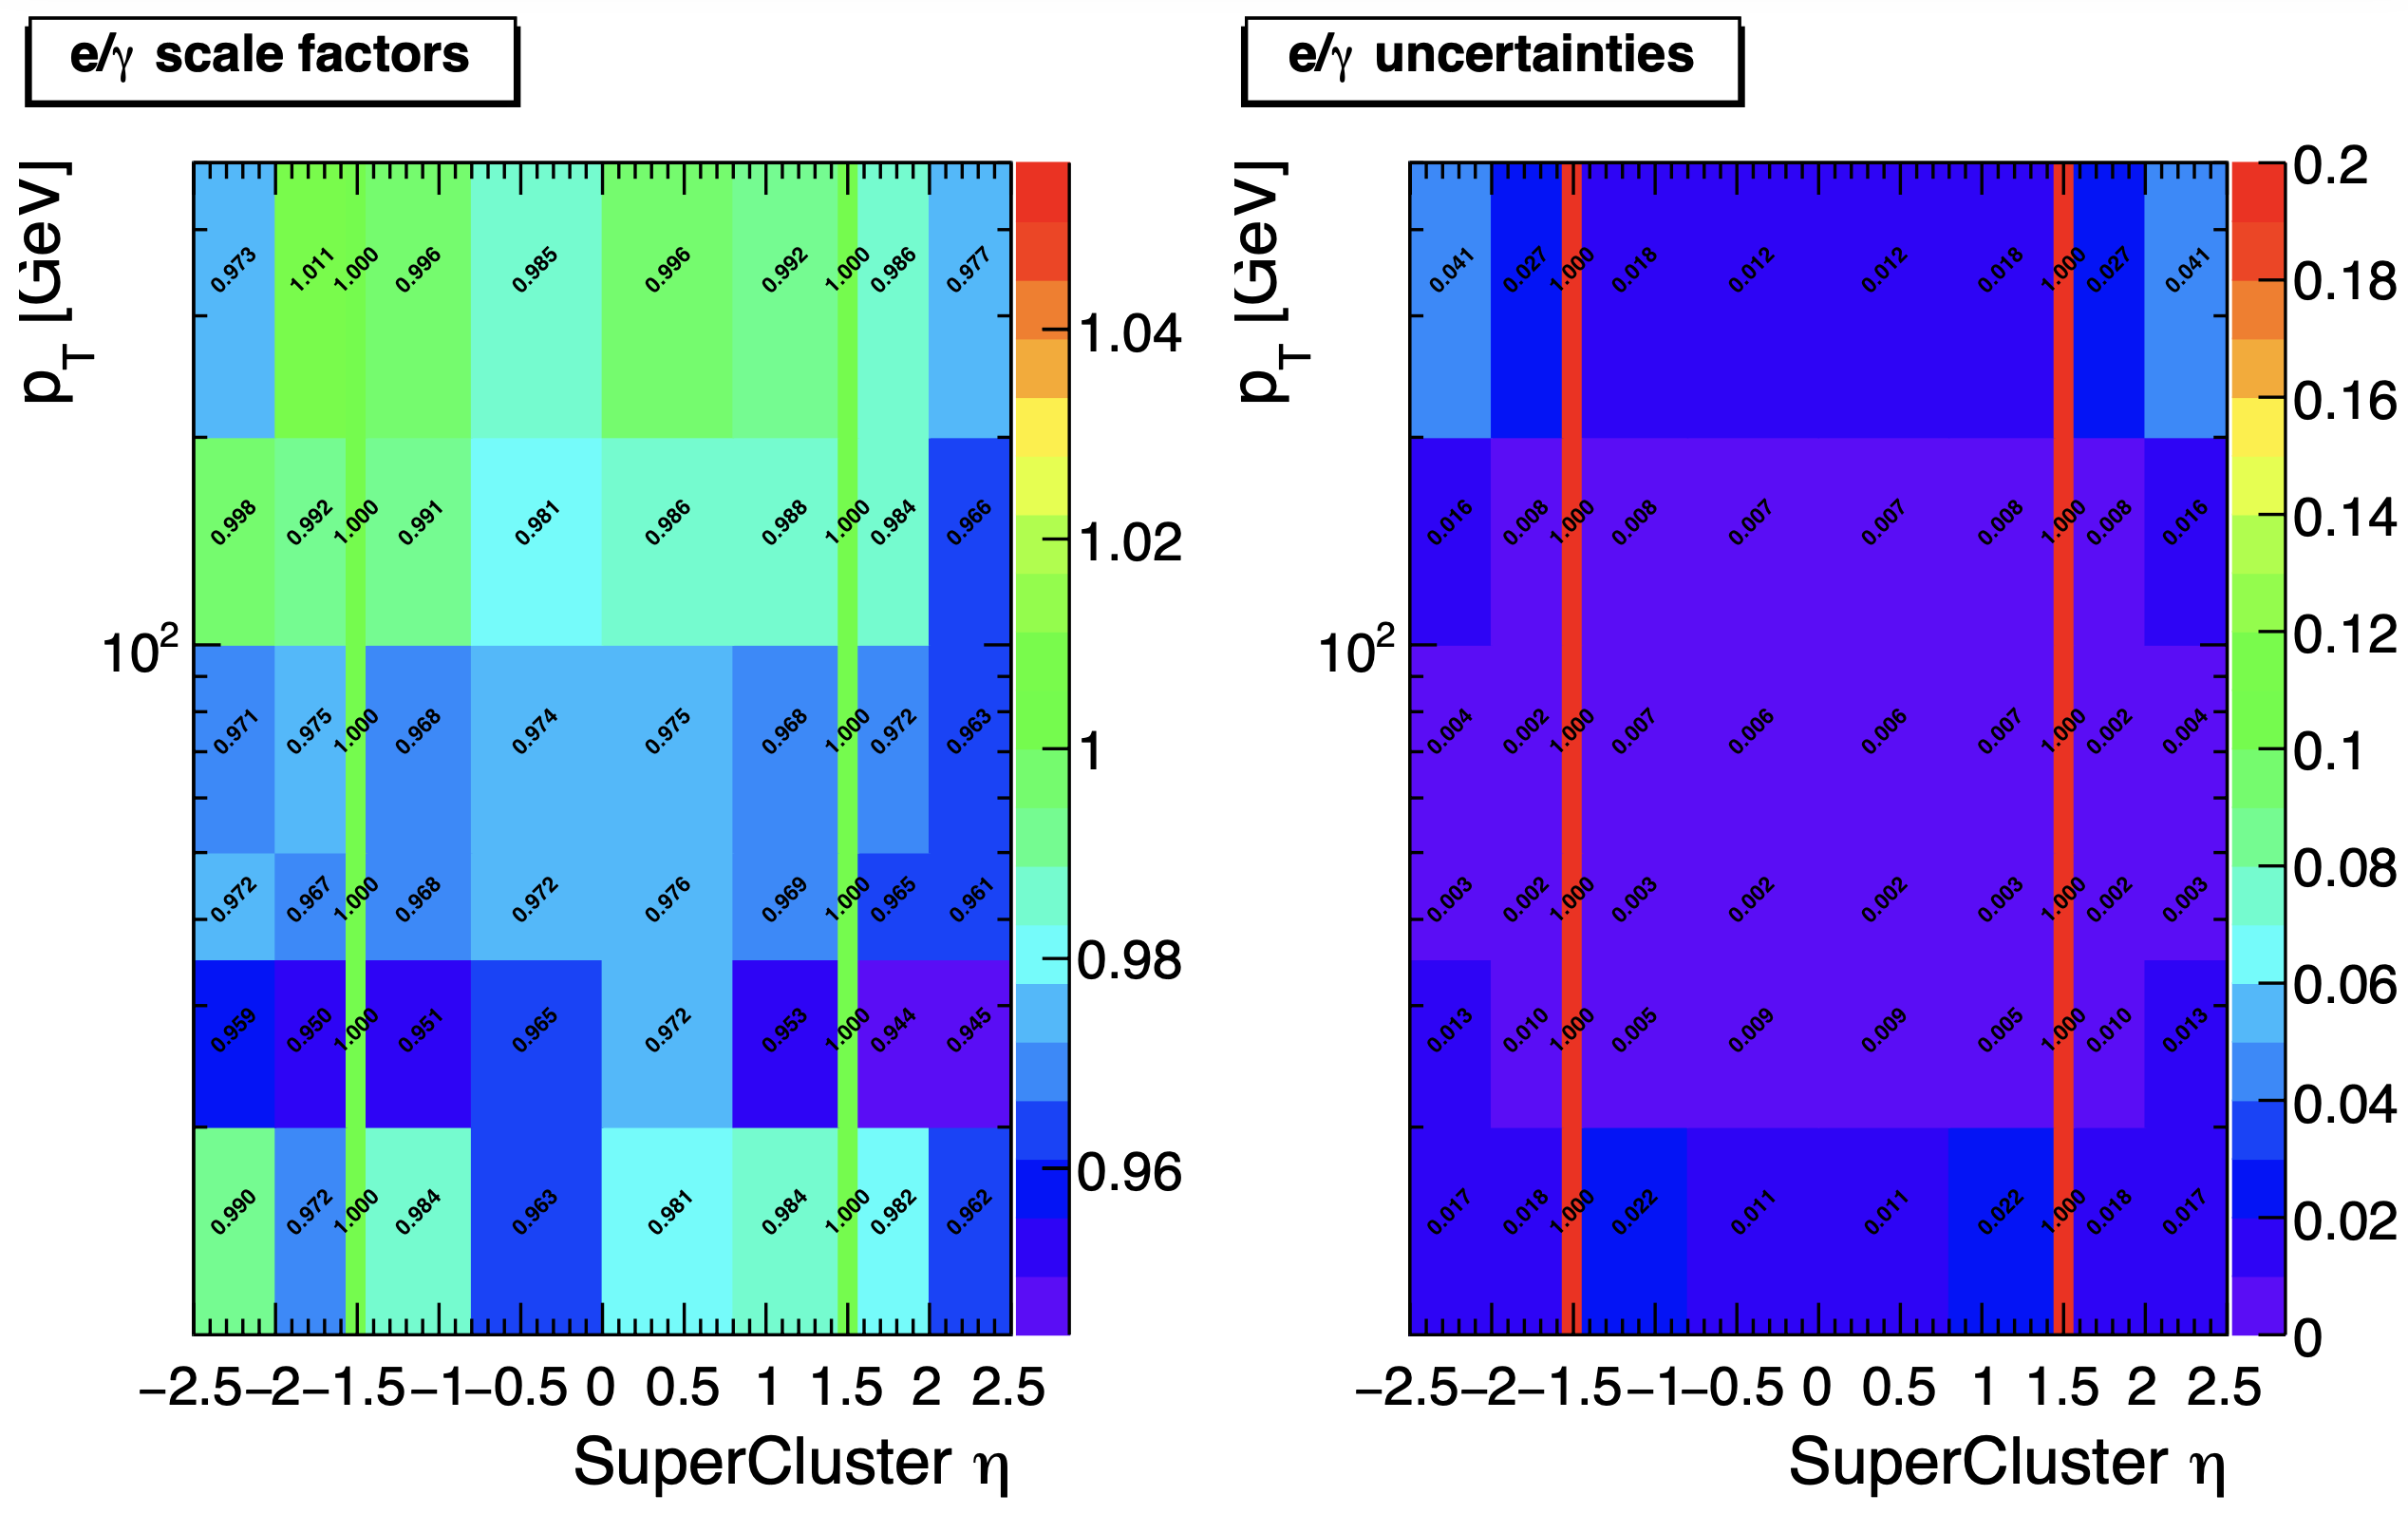
\includegraphics[width=15cm]{figures/ch-5-object-reconstruction-and-corrections-applied/egamma-POG-UL-egamma-scale-factors.png}
    \caption[Electron/photon energy scale factors and uncertainties for 2018.]{Electron/photon energy scale factors (\textit{left}) and corresponding uncertainties (\textit{right}) binned in the electron $\eta$ and $p_{T}$, for the data-taking year 2018 \cite{twiki_Electron_UL_2016_2017_2018}.} 
    \label{fig:egamma-POG-UL-egamma-scale-factors}
\end{figure}


\begin{table}[h]
    \centering
    \begin{tabular}{|c|c|c|c|}
    \hline
    \multicolumn{4}{|c|}{Electron energy scale factor for embedded samples}                                   \\ \hline
    \hline
    Eta range                   & 2018               & 2017               & 2016     \\ \hline
    $|\eta| \in [0.0, 1.479)$   & 0.973 $\pm$ 0.005  & 0.986 $\pm$ 0.009  & 0.9976 $\pm$ 0.0050 \\
    $|\eta| \in [1.479, 2.4)$   & 0.980 $\pm$ 0.0125 & 0.887 $\pm$ 0.0125 & 0.993 $\pm$ 0.0125 \\ \hline
    \end{tabular}
    \caption[Energy scales and systematic errors applied to electrons in embedded samples by data-taking year/era.]{Energy scales and systematic errors applied to electrons in embedded samples, binned in the electron $\eta$, by data-taking year \cite{twiki_embedded_preUL_2016} \cite{twiki_embedded_preUL_2017} \cite{twiki_embedded_preUL_2018}.}
    \label{table:ele-ES-embedded}
\end{table}

\subsection{\texorpdfstring{$\tau_{h}$}{tauh} identification efficiency}
\label{sec:tauh_id_efficiency}

The $\tau_{h}$ identification efficiency can differ in data and MC \cite{twiki_TAU_POG_tauidrecommendationforrun2}. Recommended corrections are provided by the Tau POG, and we use the medium DeepTau vs. jet working point values. The identification efficiency is measured in $Z \rightarrow \tau\tau$ events in the $\mu\tau_{h}$ final state, and is binned in $p_{T}$ due to clear $p_{T}$ dependence of the DeepTau ID. 


\begin{table}[h]
    \centering
    \begin{tabular}{|c|c|c|c|c|c|c|}
    \hline
    \multicolumn{7}{|c|}{Tau ID efficiency for DeepTau Medium vs. jet WP in 2018}                                   \\ \hline
    \hline
    $p_{T}$ (GeV)  & $<20$  & $(20, 25]$ & $(25, 30]$ & $(30, 35]$ & $(35, 40]$ & $(40, 500] $   \\ \hline
    Central value  & 0      & 0.945      & 0.946      & 0.916      & 0.921      & 1.005 \\
    Up value       & 0      & 1.001      & 0.981      & 0.946      & 0.950      & 1.035 \\
    Down value     & 0      & 0.888      & 0.981      & 0.883      & 0.893      & 0.953 \\ \hline
    \end{tabular}
    \caption[Tau ID efficiency for the DeepTau vs. jet medium working point, with central, up, and down values for 2018, binned in the tau $p_{T}$.]{Tau ID efficiency for the DeepTau vs. jet medium working point, with central, up, and down values for 2018, binned in the tau $p_{T}$ \cite{twiki_TAU_POG_tauidrecommendationforrun2}.}
    \label{table:tauIDeff_deepTau_vs_jet_medium_WP}
\end{table}


\subsection{Trigger efficiencies}

Scale factors are applied to correct for differences in trigger efficiencies between MC and embedded vs. data, with values taken from tools provided by the Standard Model $H \rightarrow \tau\tau$ working group which uses the same trigger paths \cite{twiki_HiggsToTauTauWorkingLegacyRun2}. In the following sections we review relevant trigger efficiencies in data, which form the basis of the trigger efficiency corrections applied to MC and embedded.

\subsection{Tau trigger efficiencies}
The efficiencies in data of the single-$\tau_{h}$ leg in $\mu\tau_{h}$, $e\tau_{h}$, and di-$\tau_{h}$ triggers is computed centrally per using a Tag and Probe (TnP) method \cite{CMS-DP-2019-012} which is outlined here. In this method, $Z \rightarrow \tau\tau \rightarrow \mu\tau_{h}$ are selected in data and a Drell-Yan simulated sample ($Z \rightarrow \ell\ell, \ell = e, \mu, \tau_{h}$) with high purity. Cuts are applied to reject events not in this final state, e.g. suppressing $Z \rightarrow \mu\mu$ by vetoing events with a single loose ID muon. An isolated muon candidate (the tag) with online $p_{T} > 27$ GeV and $|\eta| < 2.1$ is identified and matched to an offline $\mu$. An offline $\tau_{h}$ candidate (the probe) is selected, which is separated from the tag $\mu$, and has $p_{T} > 20$ GeV and $|\eta| < 2.1$. The probe $\tau_{h}$ must pass anti-muon and anti-electron discriminators to avoid fakes from muons and electrons, and must pass the medium MVA tau isolation to suppress fakes from QCD jets. The trigger efficiency in the TnP method is calculated as 
\begin{equation}
    \text{Efficiency} = \frac{\text{Number of events passing the TnP selection with fires the HLT path}}{\text{Number of events passing the TnP selection}}
\end{equation}


The efficiencies for the hadronic tau legs in the relevant channels of this analyses ($\mu\tau_{h}$ and $e\tau_{h}$) as a function of the offline tau $p_{T}$ and $\eta$, are shown for data taken in 2016, 2017, and 2018 in Figures \ref{fig:mutauEfficiencyPt_eachYear_mediumTauMVA_Data} and \ref{fig:etauEfficiencyPt_eachYear_mediumTauMVA_Data} \cite{CMS-DP-2019-012} \cite{twiki_Tau_Lepton_Run_2_trigger_performance}. In both figures, the different HLT thresholds and differences in the L1 seed result in higher efficiencies in 2016 and differences in shapes of the 2016 efficiencies compared to 2017 and 2018. The low pileup in 2016 also leads to higher efficiencies in that year.


\begin{figure}[h]
    \centering
    \begin{subfigure}{0.45\textwidth}
        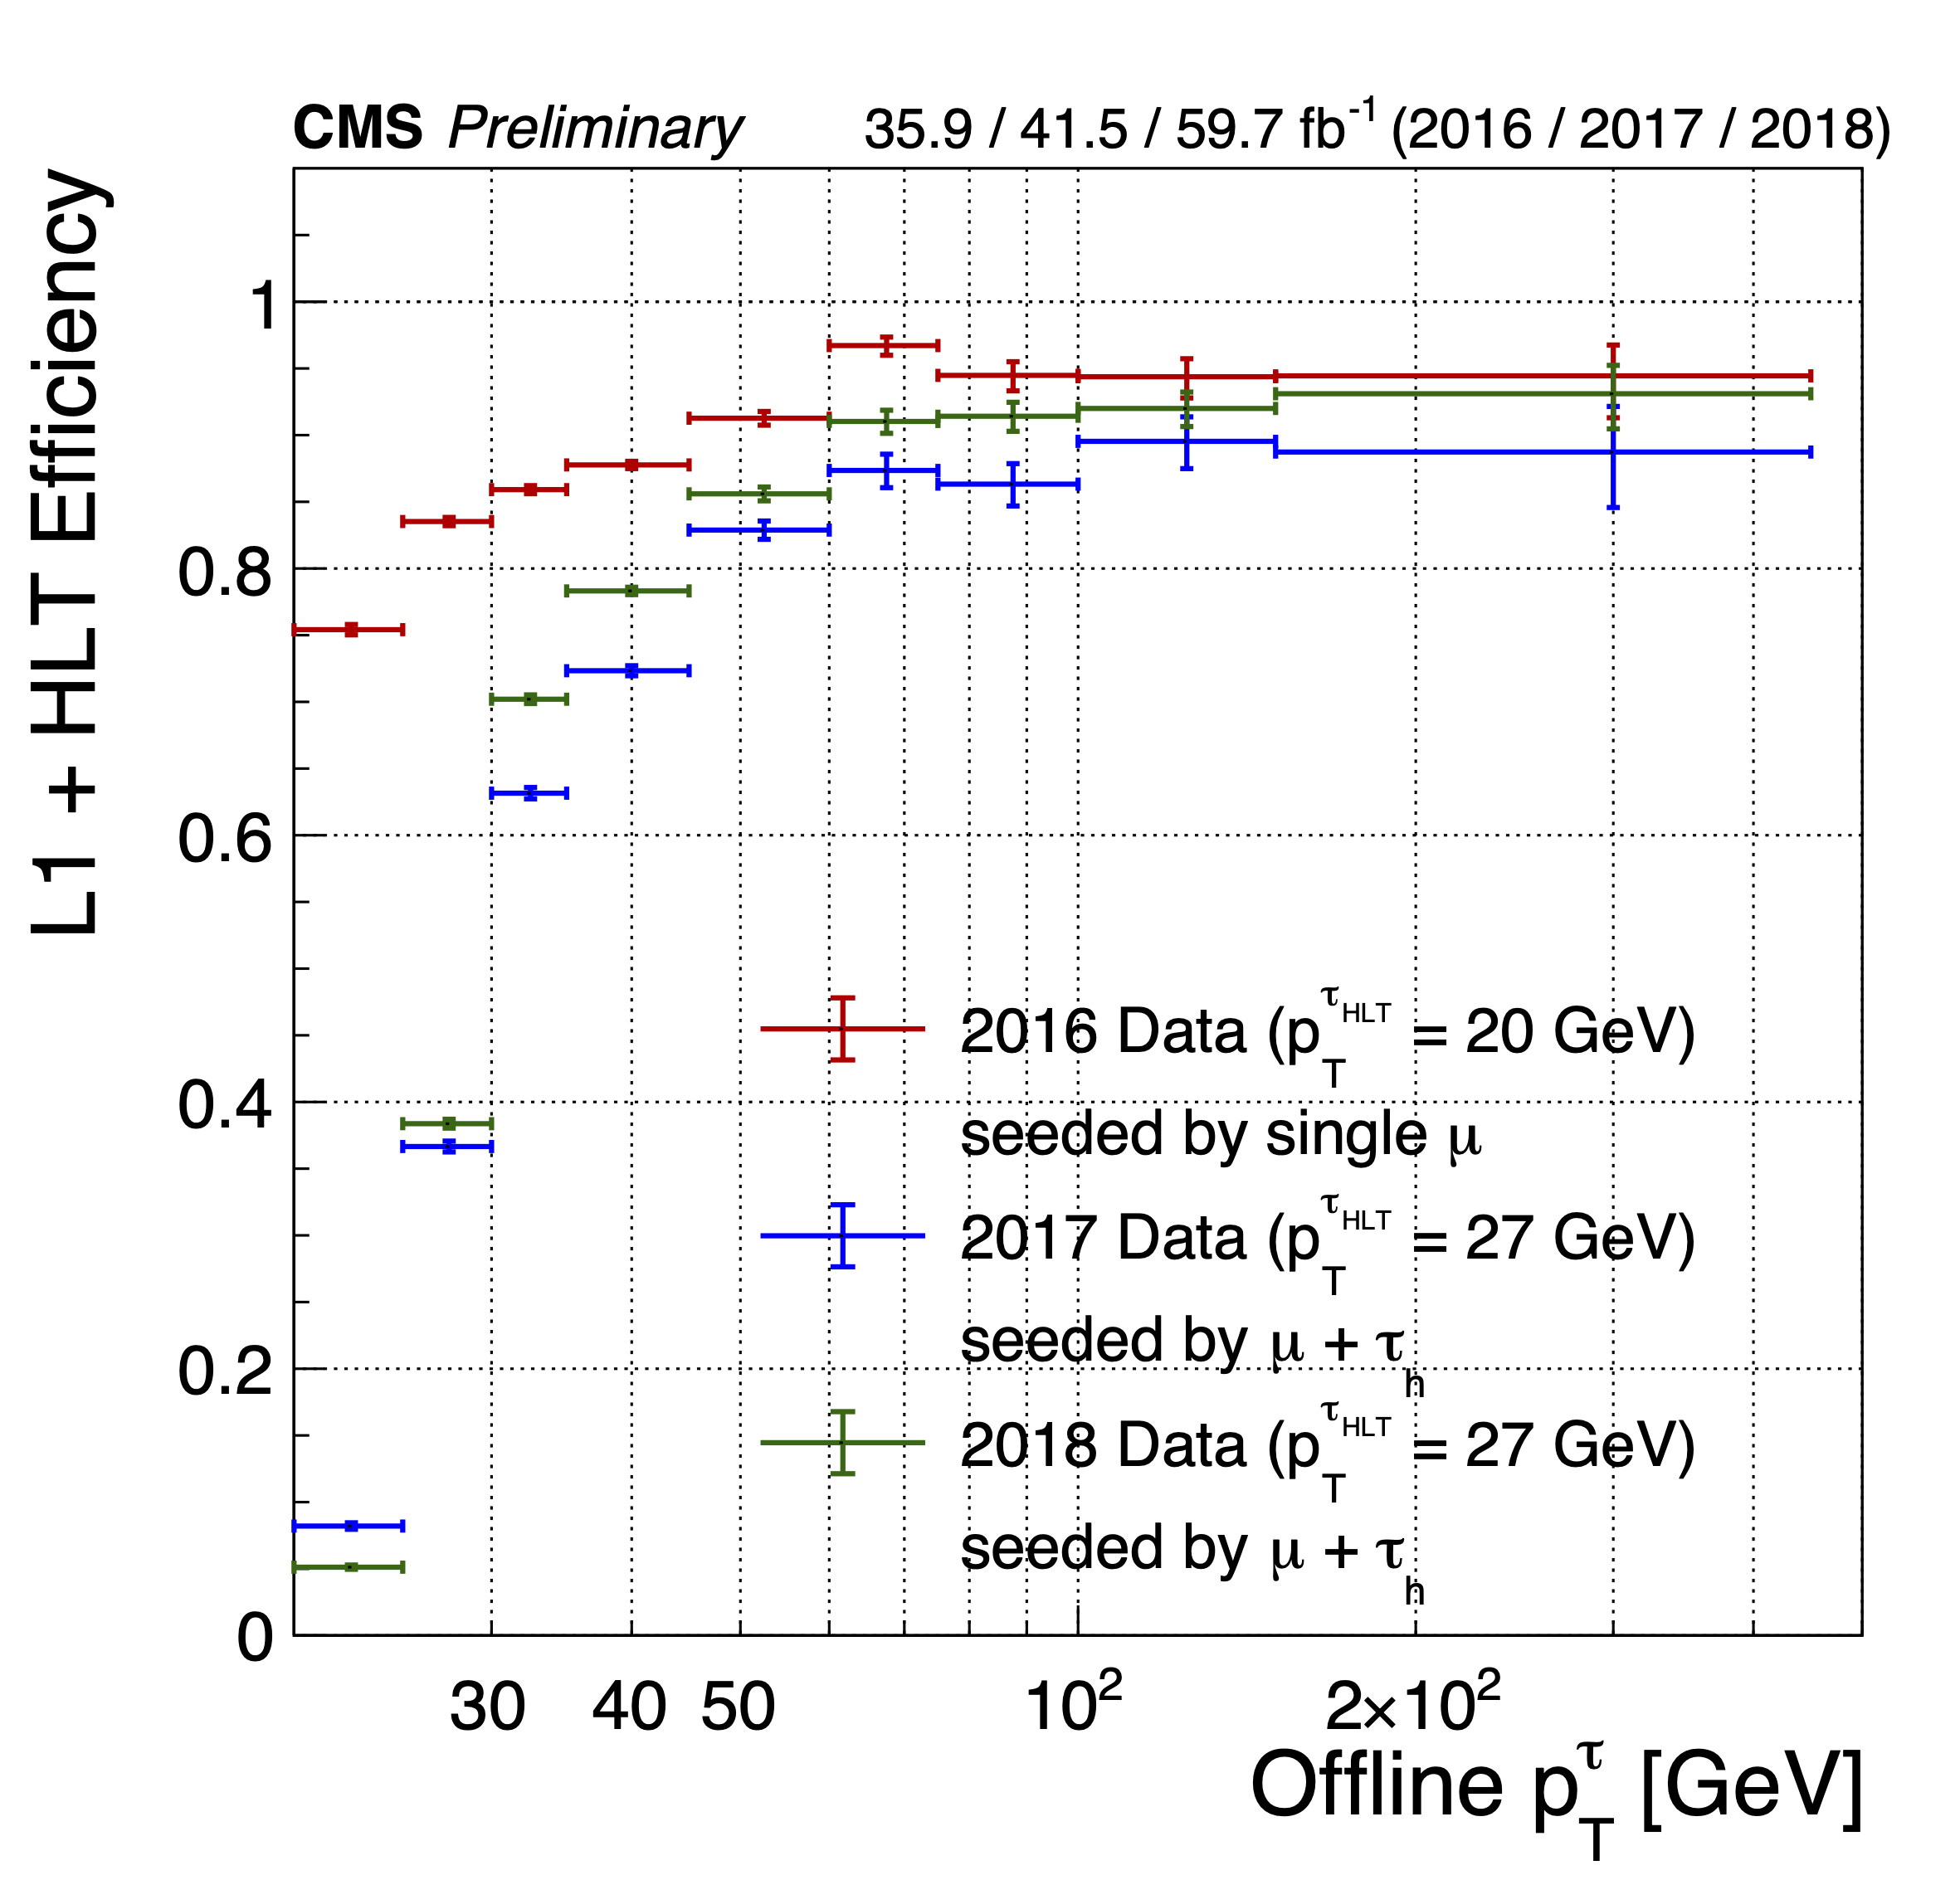
\includegraphics[width=1.0\textwidth]{figures/ch-5-object-reconstruction-and-corrections-applied/mutauEfficiencyPt_eachYear_mediumTauMVA_Data.png}
        \caption{$\tau_{h}$ efficiency from $\mu\tau_{h}$ trigger.}
        \label{fig:mutauEfficiencyPt_eachYear_mediumTauMVA_Data}
    \end{subfigure}
    \hfill
    \begin{subfigure}{0.45\textwidth}
        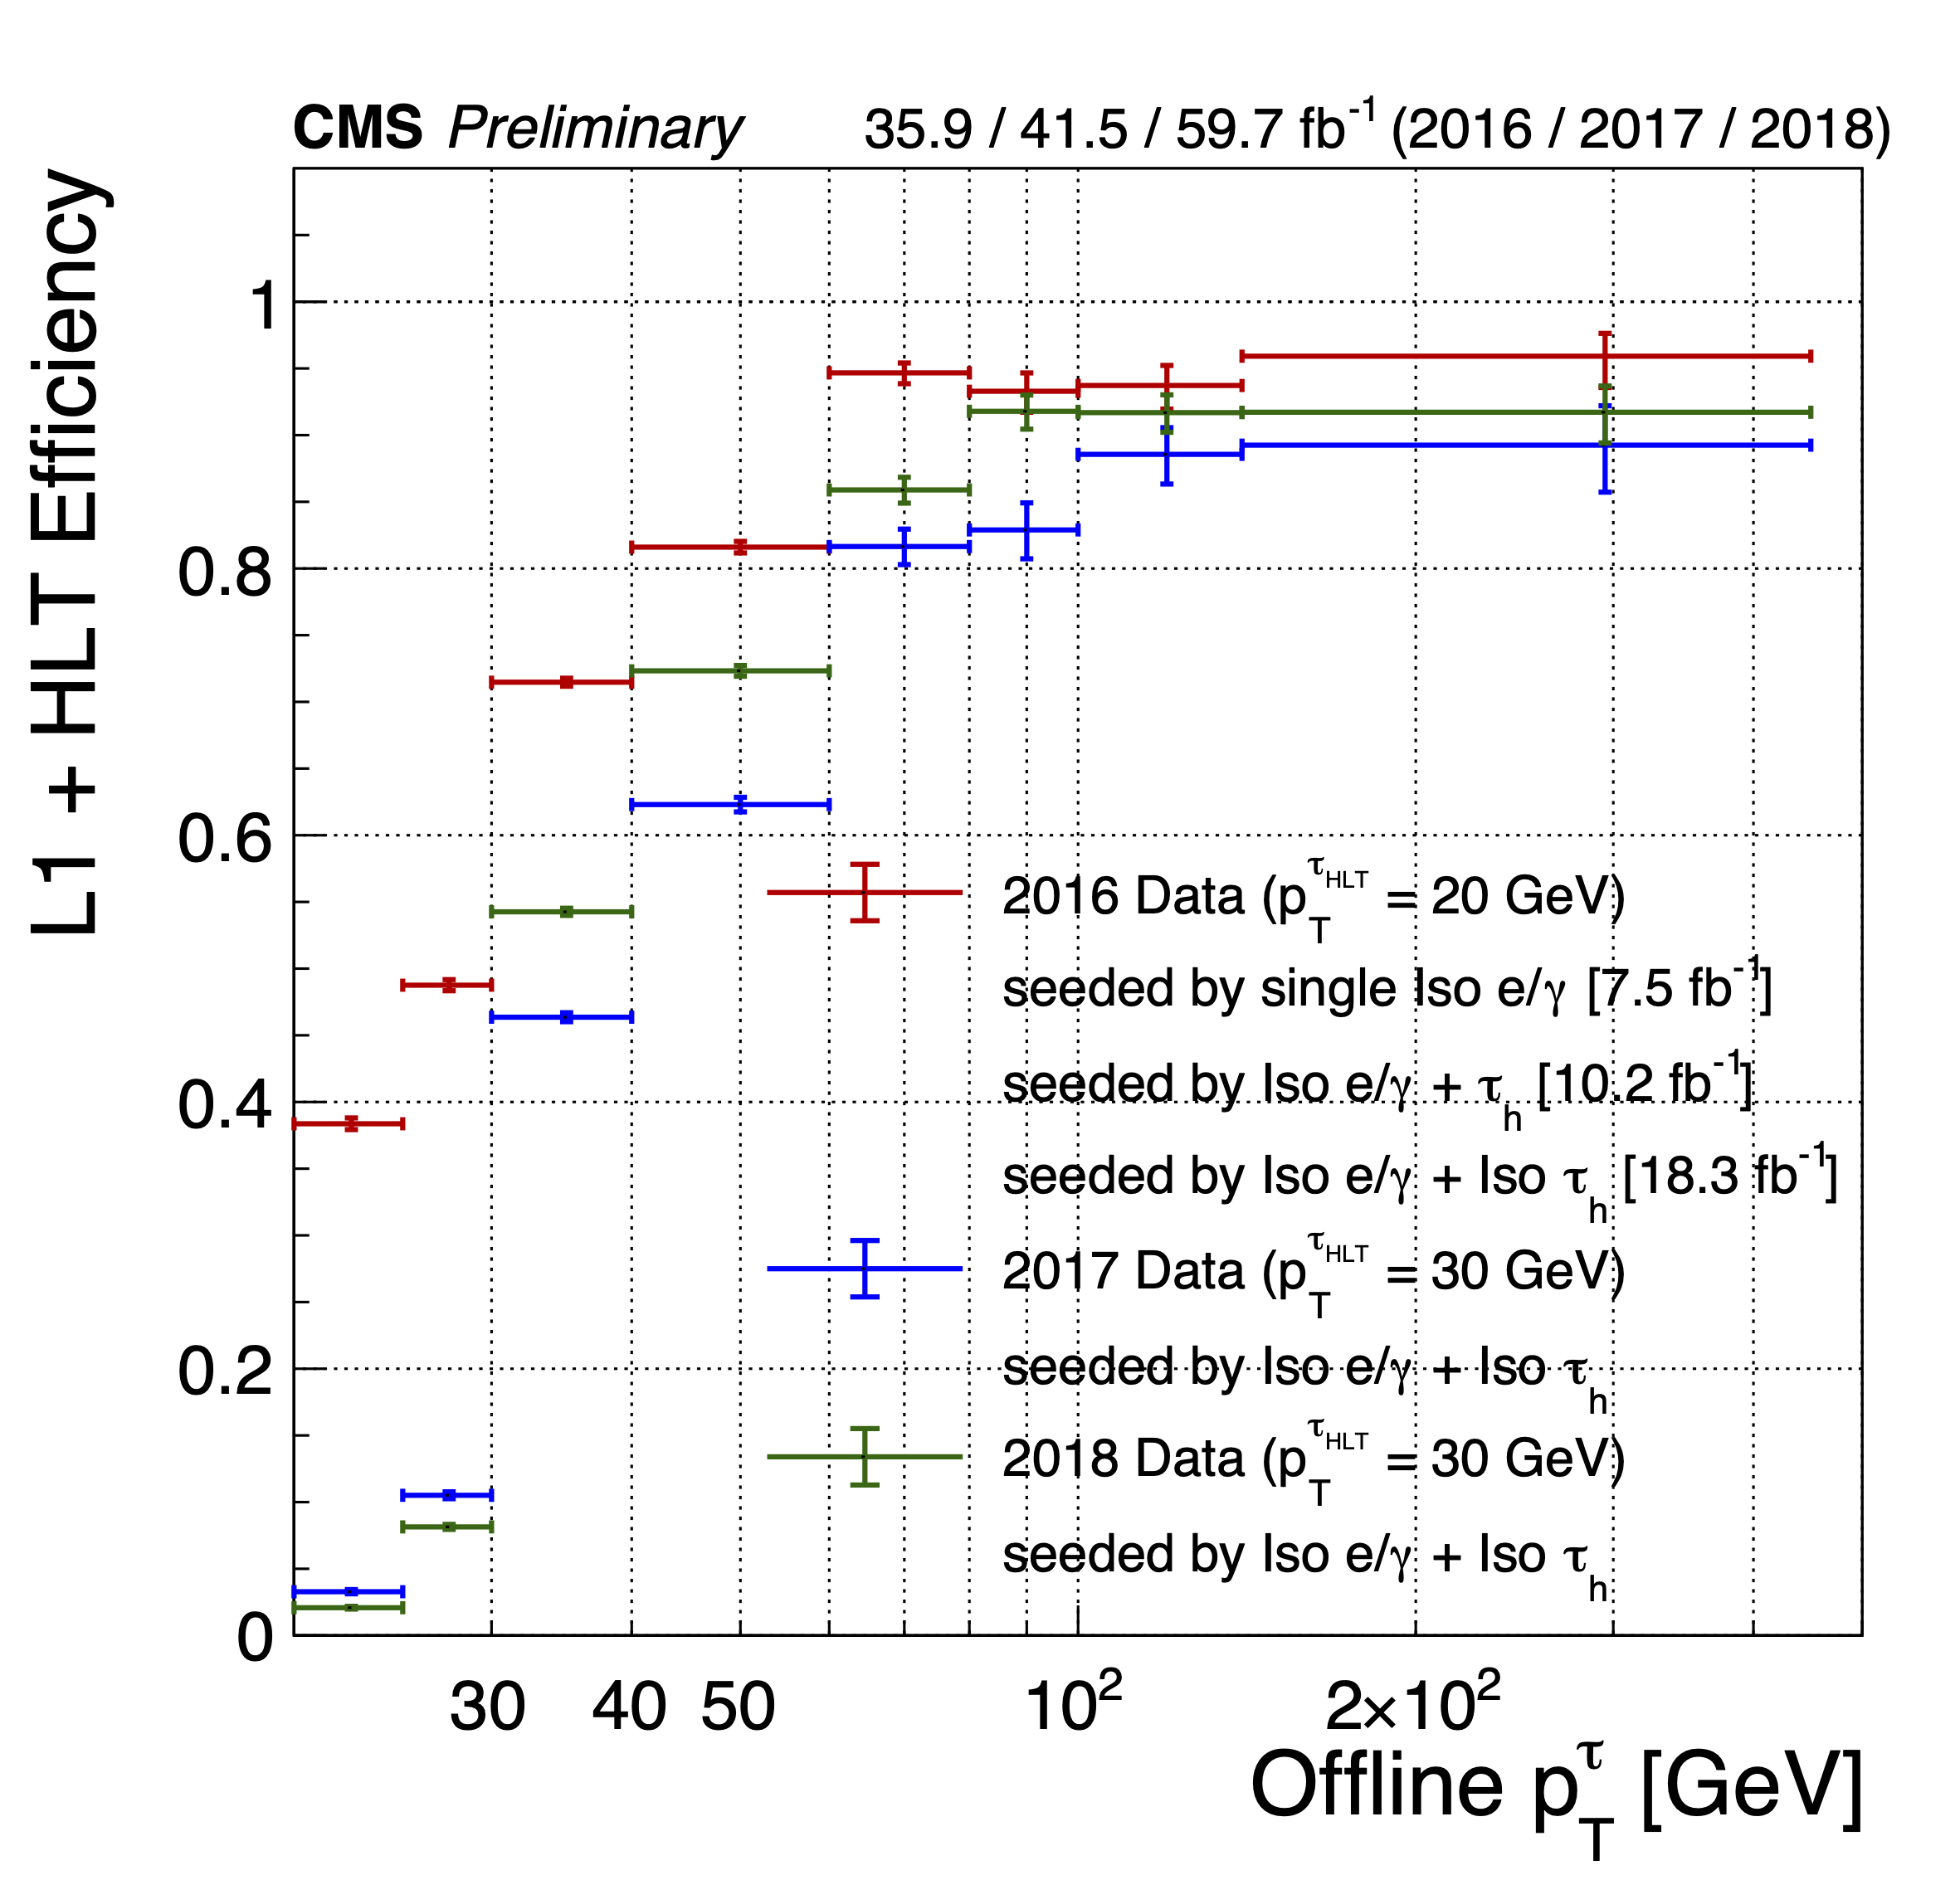
\includegraphics[width=1.0\textwidth]{figures/ch-5-object-reconstruction-and-corrections-applied/etauEfficiencyPt_eachYear_mediumTauMVA_Data.png}
        \caption{$\tau_{h}$ efficiency from $e\tau_{h}$ trigger.}
        \label{fig:etauEfficiencyPt_eachYear_mediumTauMVA_Data}
    \end{subfigure}
    \caption[Hadronic tau leg efficiency of the cross-triggers for $\mu\tau_{h}$ (\textit{left}) and $e\tau_{h}$ (\textit{right}) triggers as a function of offline tau $p_{T}$ for 2016, 2017, and 2018.]{Hadronic tau leg efficiency of the cross-triggers for $\mu\tau_{h}$ (\textit{left}) and $e\tau_{h}$ (\textit{right}) triggers as a function of offline tau $p_{T}$ for the years 2016 (\textit{red}), 2017 (\textit{blue}) and 2018 (\textit{green}), from \cite{twiki_Tau_Lepton_Run_2_trigger_performance}. HLT $p_{T}$ thresholds and L1 seeds are indicated in the legends.} 
\end{figure}


\subsection{Single muon trigger efficiencies}
The efficiencies for the single isolated muon trigger with $p_{T} > 24$ GeV used in this analysis, is shown for the data-taking year 2018 in Fig. \ref{fig:single_muon_24GeV_efficiency_vs_pt} as a function of the muon $p_{T}$ and as a function of the muon $|\eta|$ in Fig. \ref{fig:single_muon_24GeV_efficiency_vs_eta} from \cite{CMS-DP-2018-034}. The data is split with respect to a HLT muon reconstruction update that was deployed on 15/05/2018. A small asymmetry in efficiencies between negative and positive $\eta$ in Fig. \ref{fig:single_muon_24GeV_efficiency_vs_eta} is due to disabled muon chambers (CSCs). The efficiencies shown are estimated using a Tag and Probe method using $Z\rightarrow \mu\mu$ events, with the tag being an offline muon with $p_{T} > 29$ GeV and $|\eta| < 2.4$ passing a tight ID criteria, and the probe is an online (L1) trigger object with $\Delta R < 0.3$ and passing tight ID and Particle Flow based isolation requirements with $p_{T} > 26$ GeV.

\begin{figure}[h]
    \centering
    \begin{subfigure}{0.45\textwidth}
        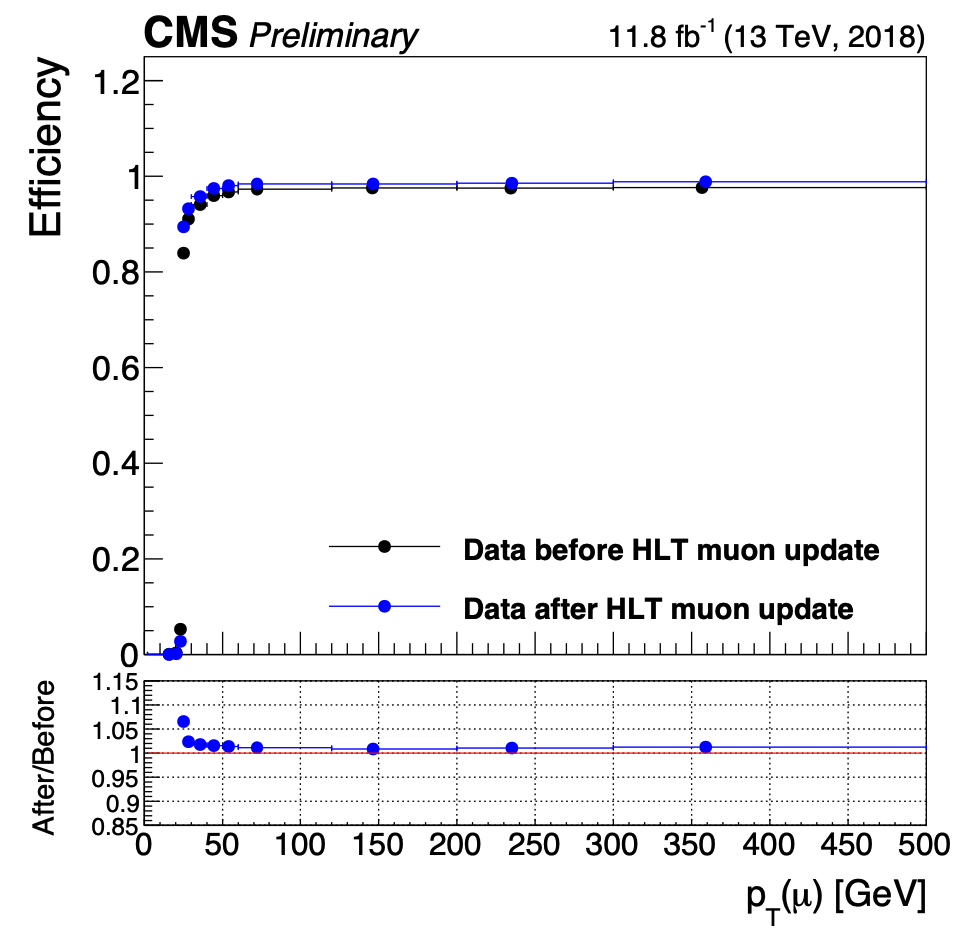
\includegraphics[width=1.0\textwidth]{figures/ch-5-object-reconstruction-and-corrections-applied/singleMuon_isolated_efficiency_vs_pt}
        \caption{Muon efficiency vs $p_{T}$ for SingleMuon.}
        \label{fig:single_muon_24GeV_efficiency_vs_pt}
    \end{subfigure}
    \hfill
    \begin{subfigure}{0.45\textwidth}
        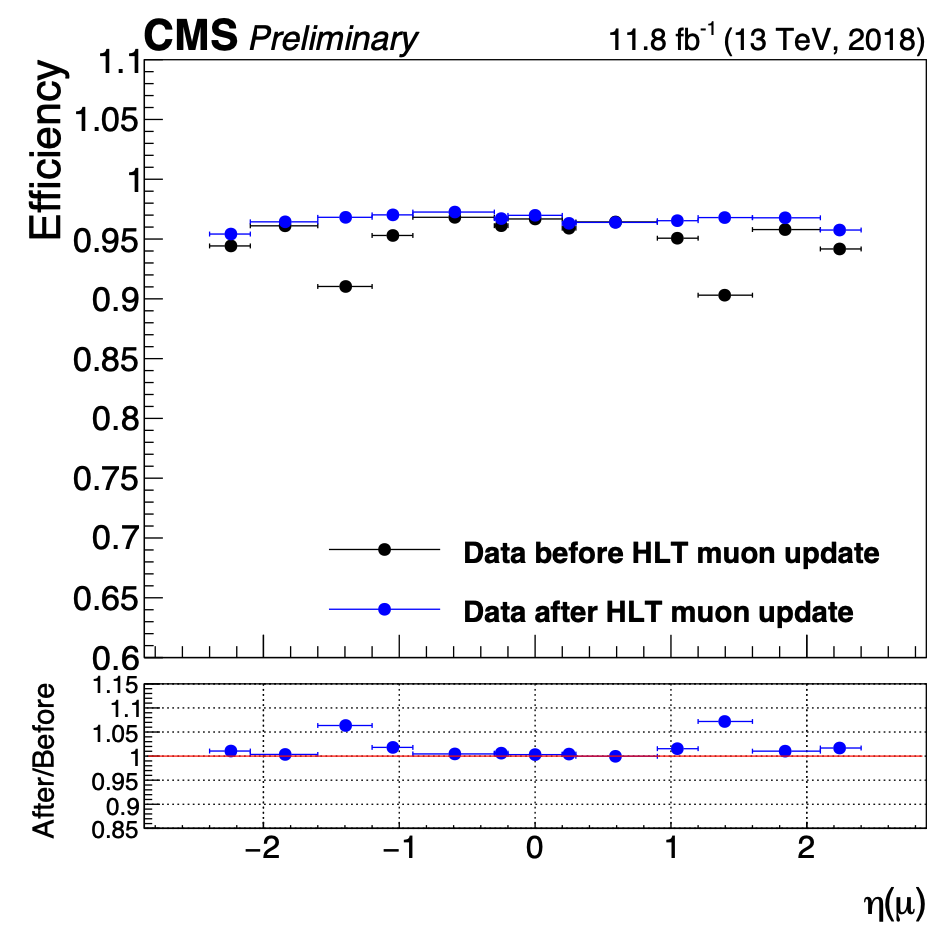
\includegraphics[width=1.0\textwidth]{figures/ch-5-object-reconstruction-and-corrections-applied/singleMuon_isolated_efficiency_vs_eta}
        \caption{Muon efficiency vs $|\eta|$ for SingleMuon.}
        \label{fig:single_muon_24GeV_efficiency_vs_eta}
    \end{subfigure}
    \caption[Trigger efficiencies in data (\textit{top panels}) and ratio of efficiencies after/before a HLT muon reconstruction update (\textit{bottom panels}) for the muon in the isolated single muon trigger with threshold $p_{T} > 24$ GeV in the data-taking year 2018, as functions of the muon $p_{T}$ (\textit{left}) and muon $|\eta|$ (\textit{right}).]{Trigger efficiencies in data (\textit{top panels}) and ratio of efficiencies after/before a HLT muon reconstruction update (\textit{bottom panels}) for the muon in the isolated single muon trigger with threshold $p_{T} > 24$ GeV in the data-taking year 2018, as functions of the muon $p_{T}$ (\textit{left}) and muon $|\eta|$ (\textit{right}). Only statistical errors are shown \cite{CMS-DP-2018-034}.} 
\end{figure}

\subsection{Single electron trigger efficiencies}

The efficiencies in data, and the ratio between data and MC, of the single electron HLT trigger with $p_{T}$ threshold 32 GeV used in this analysis are shown for 2018, as a function of the electron $p_{T}$ in Fig. \ref{fig:single_ele_32GeV_efficiency_vs_pt} and of the electron $|\eta|$ in Fig. \ref{fig:single_ele_32GeV_efficiency_vs_eta}, from \cite{CMS-DP-2020-016}. In the Tag and Probe method used for the 2018 dataset, the tag is an offline reconstructed electron with $|\eta| \leq 2.1$ and not in the barrel and endcap overlap region, with $p_{T} > 35$ GeV with tight isolation and shower shape requirements, firing the tag trigger. The probe is an offline reconstructed electron with $|\eta| \leq 2.5$ with $E_T^\text{ECAL} > 5$ GeV with no extra identification criteria \cite{CMS-DP-2020-016}. 

The disagreement between data and MC, particularly at low transverse momentum, is in part due to detector effects that are difficult to simulate, such as crystal transparency losses in the ECAL and the evolution of dead regions in the pixel tracker \cite{CMS-DP-2020-016}.

\begin{figure}[h]
    \centering
    \begin{subfigure}{0.45\textwidth}
        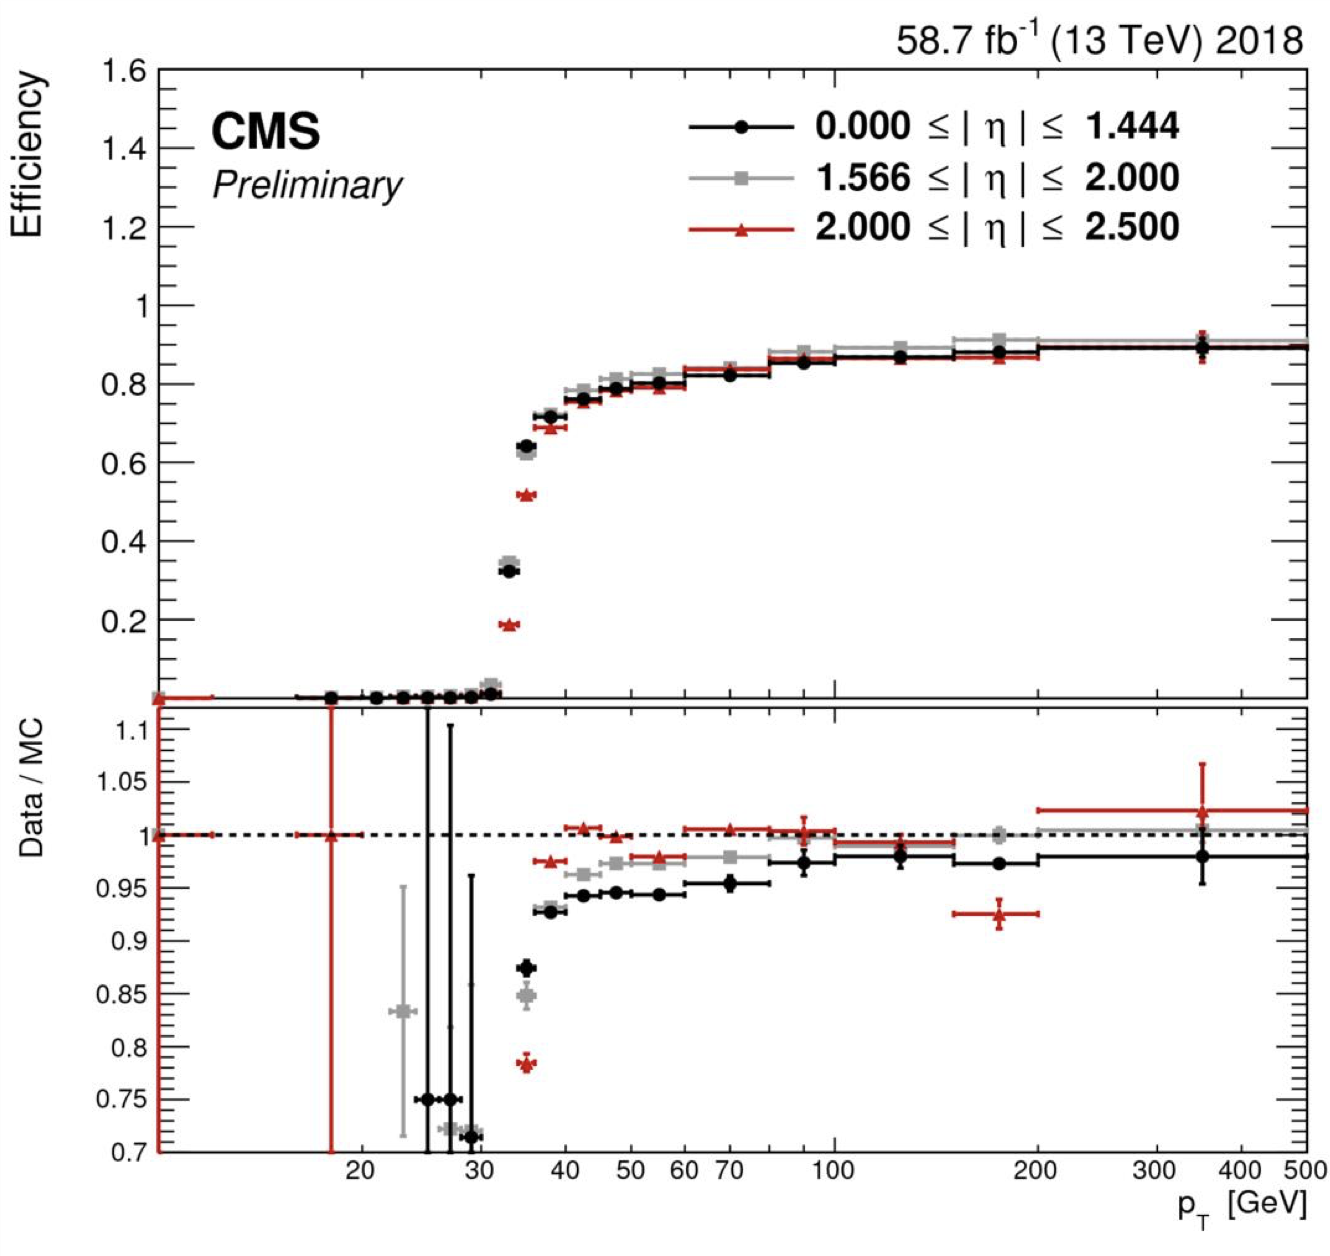
\includegraphics[width=1.0\textwidth]{figures/ch-5-object-reconstruction-and-corrections-applied/electron_Ele32_WPTight_Gsf_efficiency_vsPt}
        \caption{Electron efficiency vs $p_{T}$ for single electron.}
        \label{fig:single_ele_32GeV_efficiency_vs_pt}
    \end{subfigure}
    \hfill
    \begin{subfigure}{0.45\textwidth}
        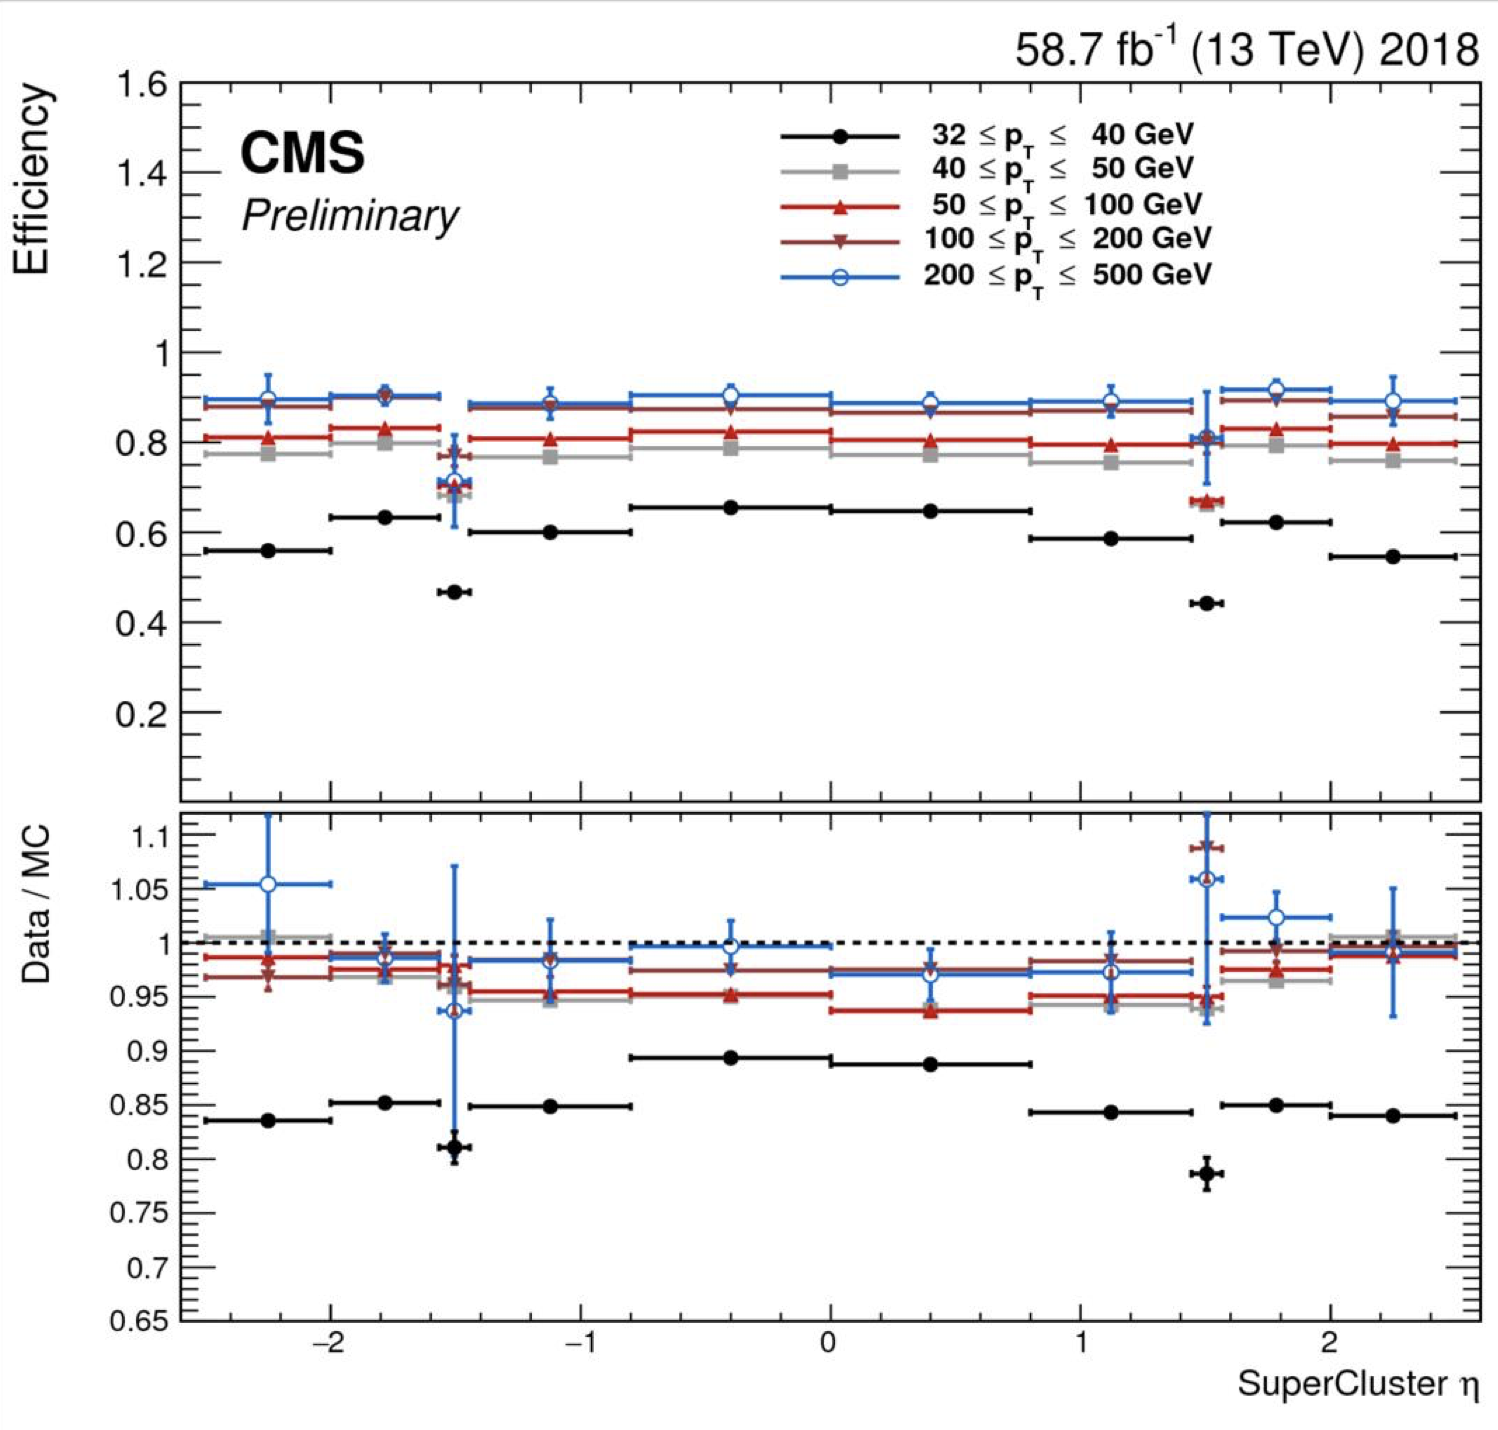
\includegraphics[width=1.0\textwidth]{figures/ch-5-object-reconstruction-and-corrections-applied/electron_Ele32_WPTight_Gsf_efficiency_vsEta}
        \caption{Electron efficiency vs $|\eta|$ for single electron.}
        \label{fig:single_ele_32GeV_efficiency_vs_eta}
    \end{subfigure}
    \caption[Trigger efficiencies in data and the data/MC ratio for the electron in the single electron trigger with threshold $p_{T} > 32$ GeV in the data-taking year 2018, as functions of the electron $p_{T}$ (\textit{left}) and electron $|\eta|$ (\textit{right}).]{Trigger efficiencies in data, and the data/MC ratio for the electron in the single electron trigger with threshold $p_{T} > 32$ GeV in the data-taking year 2018, as functions of the electron $p_{T}$ (\textit{left}) and electron $|\eta|$ (\textit{right}) \cite{CMS-DP-2020-016}. In the plot vs. $p_{T}$, the region 1.442 $\leq |\eta| \leq$ 1.566 is not included as it corresponds to the transition between barrel and endcap parts of the ECAL.} 
\end{figure}


\subsection{\texorpdfstring{$e\mu$}{emu} cross-trigger efficiencies}

The efficiencies of the electron and muons for the cross-trigger with leading muon used in the $e\mu$ channel are shown for data in 2016, 2017, and 2018 in Figures \ref{fig:ele_efficiency_vs_pT_emu} and \ref{fig:muon_efficiency_vs_eta_emu} \cite{CMS-DP-2019-025}. These efficiencies were measured centrally using a Tag and Probe in events with $Z$ to dileptons with the same flavour and opposite charge, where the tags are an isolated muon or electron, and the probe (offline) candidate is required to satisfy the same lepton selection as that of the tag candidate, be matched within $\Delta R < 0.1$ with a corresponding online trigger object, and also to pass the cross-trigger. The trigger efficiency is then:
\begin{equation}
    \text{Efficiency} = \frac{\text{Events passing lepton pair selections and probe passing trigger}}{\text{Events passing lepton pair selections}}
\end{equation}

\begin{figure}[h]
    \centering
    \begin{subfigure}{0.45\textwidth}
        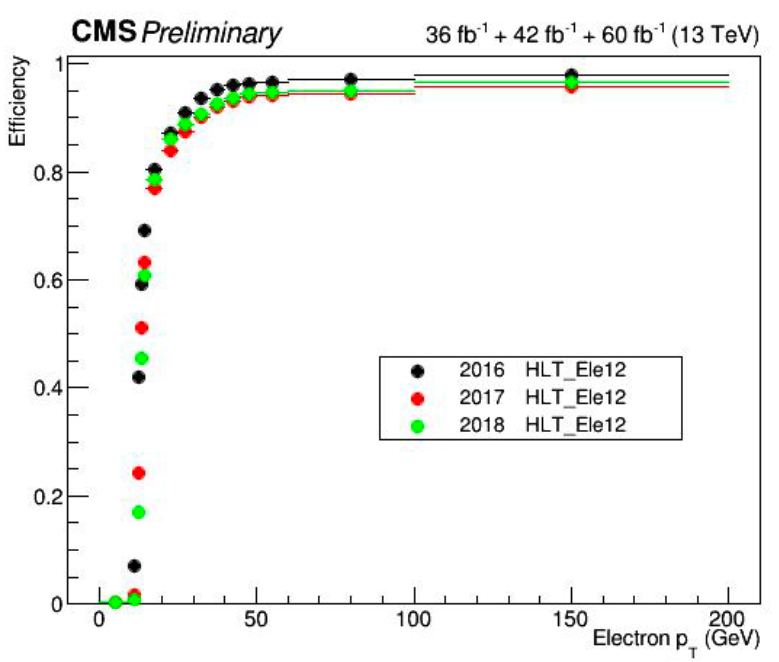
\includegraphics[width=1.0\textwidth]{figures/ch-5-object-reconstruction-and-corrections-applied/ele_efficiency_vs_pT_emu_HLT_Mu23_TrkIsoVVL_Ele12_CaloIdL_TrackIdL_IsoVL_DZ.png}
        \caption{Electron efficiency vs. $p_{T}$.}
        \label{fig:ele_efficiency_vs_pT_emu}
    \end{subfigure}
    \hfill
    \begin{subfigure}{0.45\textwidth}
        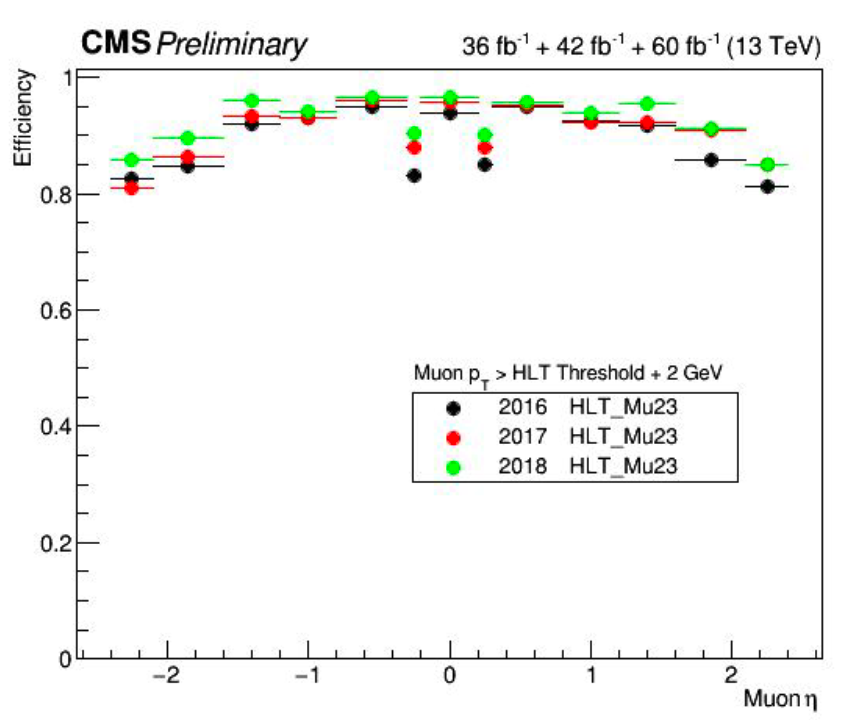
\includegraphics[width=1.0\textwidth]{figures/ch-5-object-reconstruction-and-corrections-applied/muon_efficiency_vs_eta_emu_HLT_Mu23_TrkIsoVVL_Ele12_CaloIdL_TrackIdL_IsoVL_DZ.png}
        \caption{Muon efficiency vs. $\eta$.}
        \label{fig:muon_efficiency_vs_eta_emu}
    \end{subfigure}
    \caption[Efficiencies of the electron leg vs. $p_{T}$ (\textit{left}) and the muon log vs. $\eta$ (\textit{right}), for the HLT path with online thresholds of 12 GeV for the electron and 23 GeV for the muon, with the data-taking years 2016 through 2018 overlaid.]{Efficiencies of the electron leg vs. $p_{T}$ (\textit{left}) and the muon log vs. $\eta$ (\textit{right}), for the HLT path with online thresholds of 12 GeV for the electron and 23 GeV for the muon, for the data-taking years 2016 (\textit{black}), 2017 (\textit{red}), and 2018 (\textit{green}) \cite{CMS-DP-2019-025}.} 
\end{figure}


\subsection{Electrons and muons faking \texorpdfstring{$\tau_{h}$}{tauh}: energy scales}

Energy scales for electrons misidentified as hadronic tau decays ($e$ faking $\tau_{h}$) are provided by the Tau POG, and were measured in the $e\tau_{h}$ channel with the visible invariant mass of the electron and hadronic tau system \cite{twiki_HiggsToTauTauWorkingLegacyRun2}. This energy scale is applied for $\tau_{h}$ with $p_{T} > 20$ GeV regardless of which DeepTau vs. electron working point was used. Values for 2018 are shown in Table \ref{table:electron-faking-tauh-FES-2018}.

% root -l TauFES_eta-dm_DeepTau2017v2p1VSe_2018ReReco.root 
\begin{table}[h]
    \centering
    \begin{tabular}{|c|c|}
    \hline
    \multicolumn{2}{|c|}{Electrons faking $\tau_{h}$ energy scale factor in 2018}      \\ \hline
    \hline
    Reconstructed decay mode of the fake $\tau_{h}$  & Central value and (up, down) shifts \\ \hline
    0   & 1.01362 (+0.00474, -0.00904) \\
    1   & 1.01945 (+0.01598, -0.01226) \\
    10  & 0.96903 (+0.0125, -0.03404) \\
    11 & 0.985 (+0.04309, -0.05499) \\ \hline
    \end{tabular}
    \caption[Energy scales and up/down systematic uncertainties applied to electrons misidentified as hadronic taus.]{Energy scales and up/down systematic uncertainties applied to electrons misidentified as hadronic taus for 2018, binned in decay mode of the fake $\tau_{h}$ \cite{twiki_HiggsToTauTauWorkingLegacyRun2}.}
    \label{table:electron-faking-tauh-FES-2018}
\end{table}

No nominal energy scale is applied for muons mis-reconstructed as $\tau_{h}$, and the uncertainty is treated as $\pm$ 1\% and uncorrelated in the reconstructed decay mode \cite{twiki_HiggsToTauTauWorkingLegacyRun2}. 

\subsection{Electrons and muons faking \texorpdfstring{$\tau_{h}$}{tauh}: misidentification efficiencies}
Corrections on identification efficiencies are applied to genuine electrons and muons misidentified as $\tau$ to account for differences in data and MC.

The specific values depend on the vs. electron and vs. muon discriminator working points used. 
For misidentified $\mu \rightarrow \tau_{h}$, the scale factors are split into different $|\eta|$ regions, determined by the CMS muon and tracker detector geometries, as shown in Table \ref{table:tauIDeff_deepTau_vs_muon} for 2018 \cite{twiki_TAU_POG_tauidrecommendationforrun2}.


\begin{table}[h]
    \centering
    \begin{tabular}{|c|c|c|}
    \hline
    \multicolumn{3}{|c|}{Tau ID efficiency for DeepTau vs. muon WPs in 2018} \\ \hline
    \hline
    $|\eta|$  & Tight working point & VLoose working point \\ \hline
    (0.0, 0.2)     & 0.767 $\pm$ 0.127  & 0.954 $\pm$ 0.069  \\ \hline 
    (0.2, 0.6)     & 1.255 $\pm$ 0.258  & 1.009 $\pm$ 0.098  \\ \hline 
    (0.6, 1.0)     & 0.902 $\pm$ 0.203  & 1.029 $\pm$ 0.075 \\ \hline 
    (1.0, 1.45)    & 0.833 $\pm$ 0.415  & 0.928 $\pm$ 0.145\\ \hline
    (1.45, 2.0)    & 4.436 $\pm$ 0.814   & 5.000 $\pm$ 0.377 \\ \hline
    (2.0, 2.53)    & 1.000 $\pm$ 0.000         & 1.000 $\pm$ 0.000\\ \hline
    \end{tabular}
    \caption[Tau mis-identification efficiency for the DeepTau Tight and Very Loose (VLoose) working points vs. muons in 2018.]{Tau mis-identification efficiency for the DeepTau Tight and Very Loose (VLoose) working points vs. muons in 2018, binned in the muon $|\eta|$ \cite{twiki_TAU_POG_tauidrecommendationforrun2}.}
    \label{table:tauIDeff_deepTau_vs_muon}
\end{table}

For misidentified $e \rightarrow \tau_{h}$, the scale factors are split into barrel and endcap regions, dictated by the ECAL detector geometry, as shown in Table \ref{table:tauIDeff_deepTau_vs_electron} for 2018.

% root -l /Users/stephaniekwan/Dropbox/Princeton_G6/TauIDSFs/data/TauID_SF_eta_DeepTau2017v2p1VSe_2018ReReco.root 
\begin{table}[h]
    \centering
    \begin{tabular}{|c|c|c|}
    \hline
    \multicolumn{3}{|c|}{Tau ID efficiency for DeepTau vs. electron WPs in 2018} \\ \hline
    \hline
    $|\eta|$  & Tight working point & VLoose working point \\ \hline
    (0.0, 0.73)     & 1.47 $\pm$ 0.27  & 0.95 $\pm$ 0.07  \\ \hline 
    (0.73, 1.509)   & 1.509 $\pm$ 0.0  & 1.00 $\pm$ 0.0  \\ \hline 
    (1.509, 1.929)  & 1.929 $\pm$ 0.2  & 0.86 $\pm$ 0.1 \\ \hline 
    (1.929, 2.683)  & 2.683 $\pm$ 0.9  & 2.68 $\pm$ 0.0 \\ \hline
    \end{tabular}
    \caption[Tau mis-identification efficiency for the DeepTau Tight and Very Loose (VLoose) working points vs. electrons in 2018.]{Tau mis-identification efficiency for the DeepTau Tight and Very Loose (VLoose) working points vs. electrons in 2018, binned in the electron $|\eta|$ \cite{twiki_TAU_POG_tauidrecommendationforrun2}.}
    \label{table:tauIDeff_deepTau_vs_electron}
\end{table}


\subsection{Electron ID and tracking efficiency}
Scale factors are applied to MC to correct for differences between MC and data in the performance of electron identification (ID) and tracking.

Electron and photon identification, as discussed earlier, use variables with good signal vs. background discrimination power such as lateral shower shape and ratio of energy deposited in the HCAL to energy deposited in the ECAL at the position of the electron. The cut-based electron identification efficiencies in data and ratio of efficiencies in data to MC are shown in Fig. \ref{fig:electron_MVA_ID_efficiency} for the multivariate analysis (MVA) identification working point. 

The tracking efficiencies in data and the data/MC ratio are shown in Fig. \ref{fig:electron_GSF_tracking_efficiency} for the Gaussian-sum filter (GSF) tracking \cite{CMS-DP-2020-037}. 

\begin{figure}[h]
    \centering
    \begin{subfigure}{0.45\textwidth}
        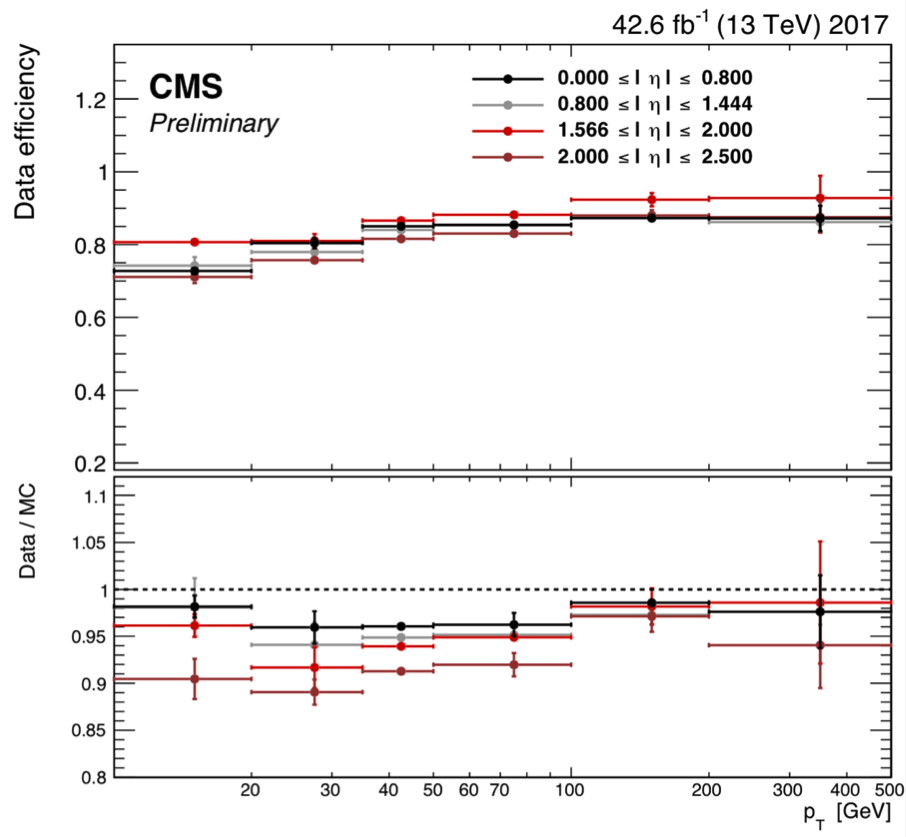
\includegraphics[width=1.0\textwidth]{figures/ch-5-object-reconstruction-and-corrections-applied/electron_MVA_90wp_identification_efficiency}
        \caption{Electron MVA ID.}
        \label{fig:electron_MVA_ID_efficiency}
    \end{subfigure}
    \hfill
    \begin{subfigure}{0.45\textwidth}
        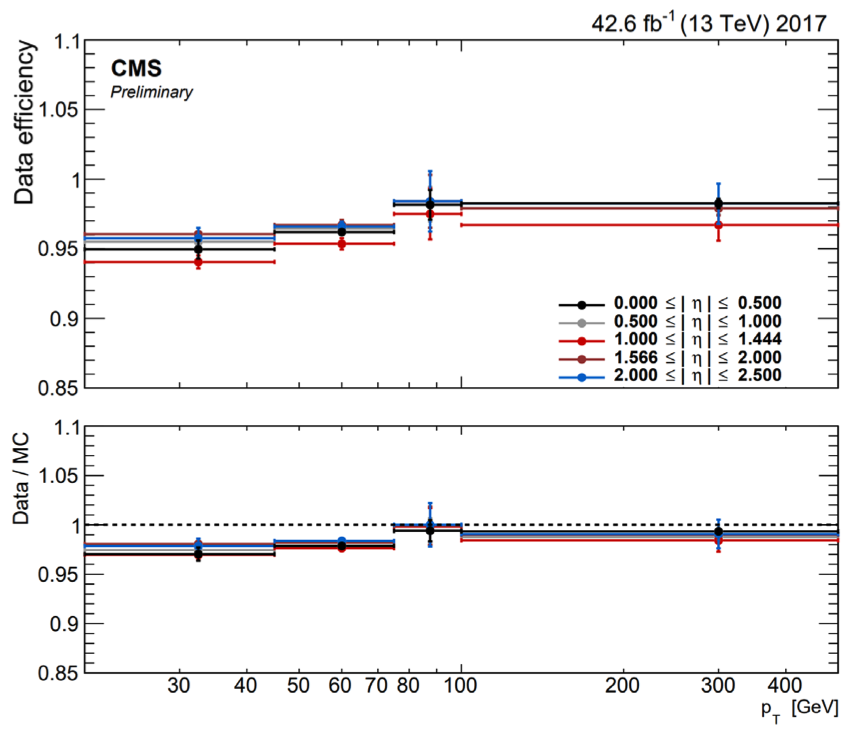
\includegraphics[width=1.0\textwidth]{figures/ch-5-object-reconstruction-and-corrections-applied/electron_gsf_tracking_efficiency}
        \caption{Electron GSF tracking.}
        \label{fig:electron_GSF_tracking_efficiency}
    \end{subfigure}
    \caption[Efficiencies in data (\textit{top panels}) and the ratio of efficiencies in data/MC (\textit{bottom panels}), for the electron multivariate analysis (MVA) identification (\textit{left}) and for the Gaussian-sum filter (GSF) tracking (\textit{right}).]{Efficiencies in data (\textit{top panels}) and the ratio of efficiencies in data/MC (\textit{bottom panels}), for the electron multivariate analysis (MVA) identification (\textit{left}) and for the Gaussian-sum filter (GSF) tracking (\textit{right}) \cite{CMS-DP-2020-037}. Error bars represent statistical and systematic uncertainties.} 
\end{figure}


\subsection{Muon ID, isolation, and tracking efficiencies}
Scale factors are applied to MC to correct for differences between MC and data in the performance of muon identification, isolation, and tracking, as detailed below.

The efficiencies for muon identification measured in 2015 data and MC simulation are shown in Figures \ref{fig:muon_looseID_efficiency} and \ref{fig:muon_tightID_efficiency} for the loose ID and tight ID respectively \cite{CMS-MUO-16-001}. The loose ID is chosen such that efficiency exceeds 99\% over the full $\eta$ range, and the data and simulation agree to within 1\%. The tight ID is chosen such that efficiency varies between 95\% and 99\% as a function of $\eta$, and the data and simulation agree to within 1-3\%. The muon identification working point used in this analysis is the medium ID, which has an efficiency of 98\% for all $\eta$ and an agreement within 1-2\% \cite{CMS-MUO-16-001}. 

\begin{figure}[h]
    \centering
    \begin{subfigure}{0.45\textwidth}
        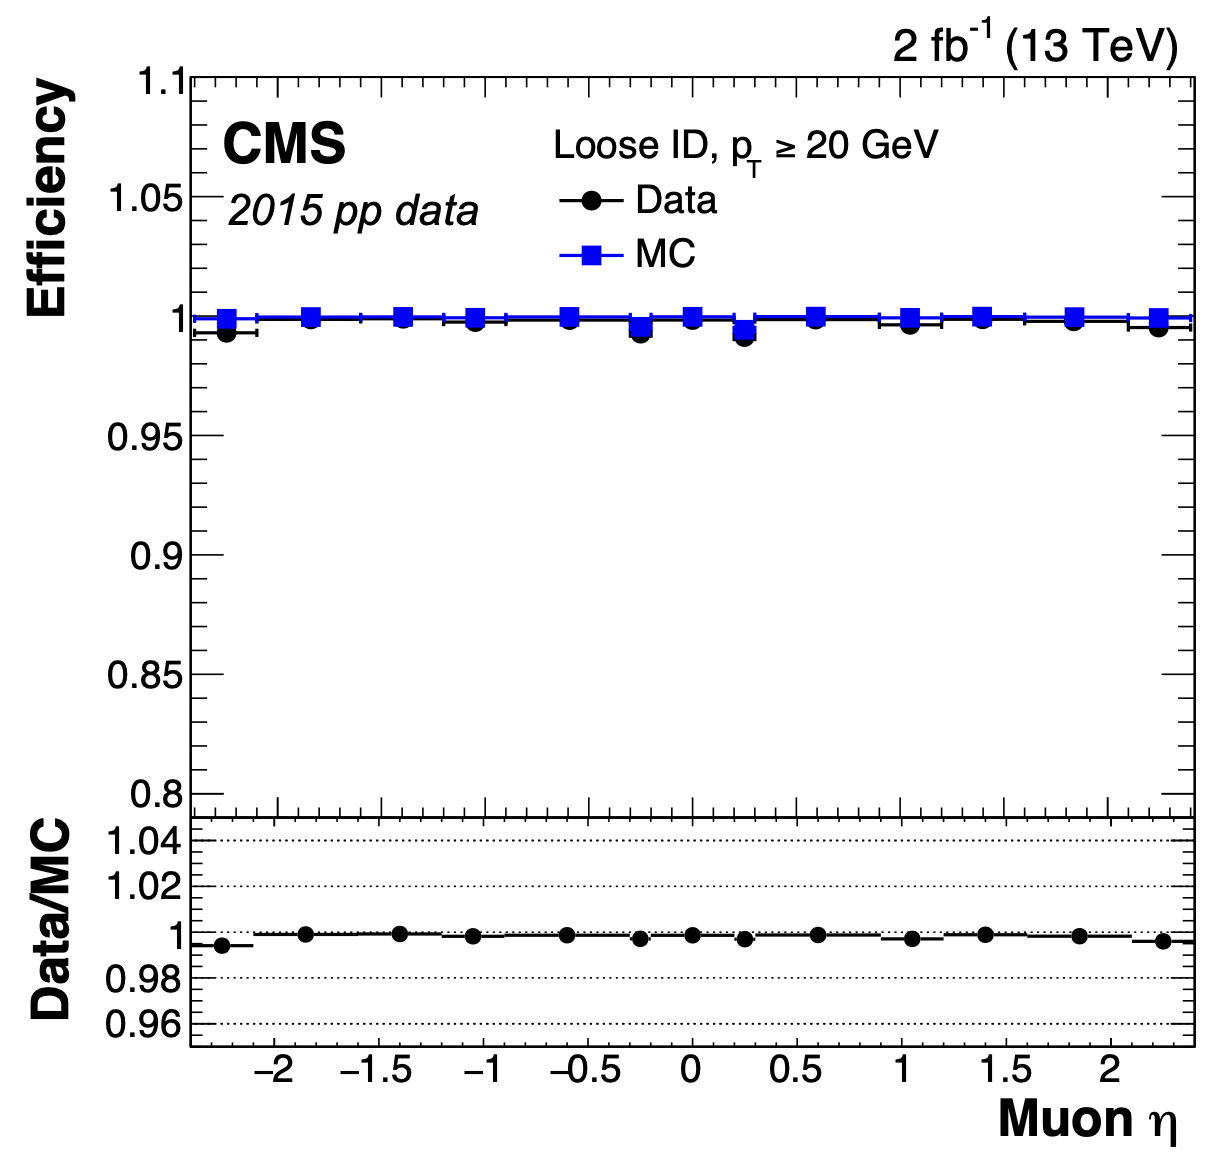
\includegraphics[width=1.0\textwidth]{figures/ch-5-object-reconstruction-and-corrections-applied/muon_efficiency_looseID}
        \caption{Muon efficiency isolation vs $p_{T}$.}
        \label{fig:muon_looseID_efficiency}
    \end{subfigure}
    \hfill
    \begin{subfigure}{0.45\textwidth}
        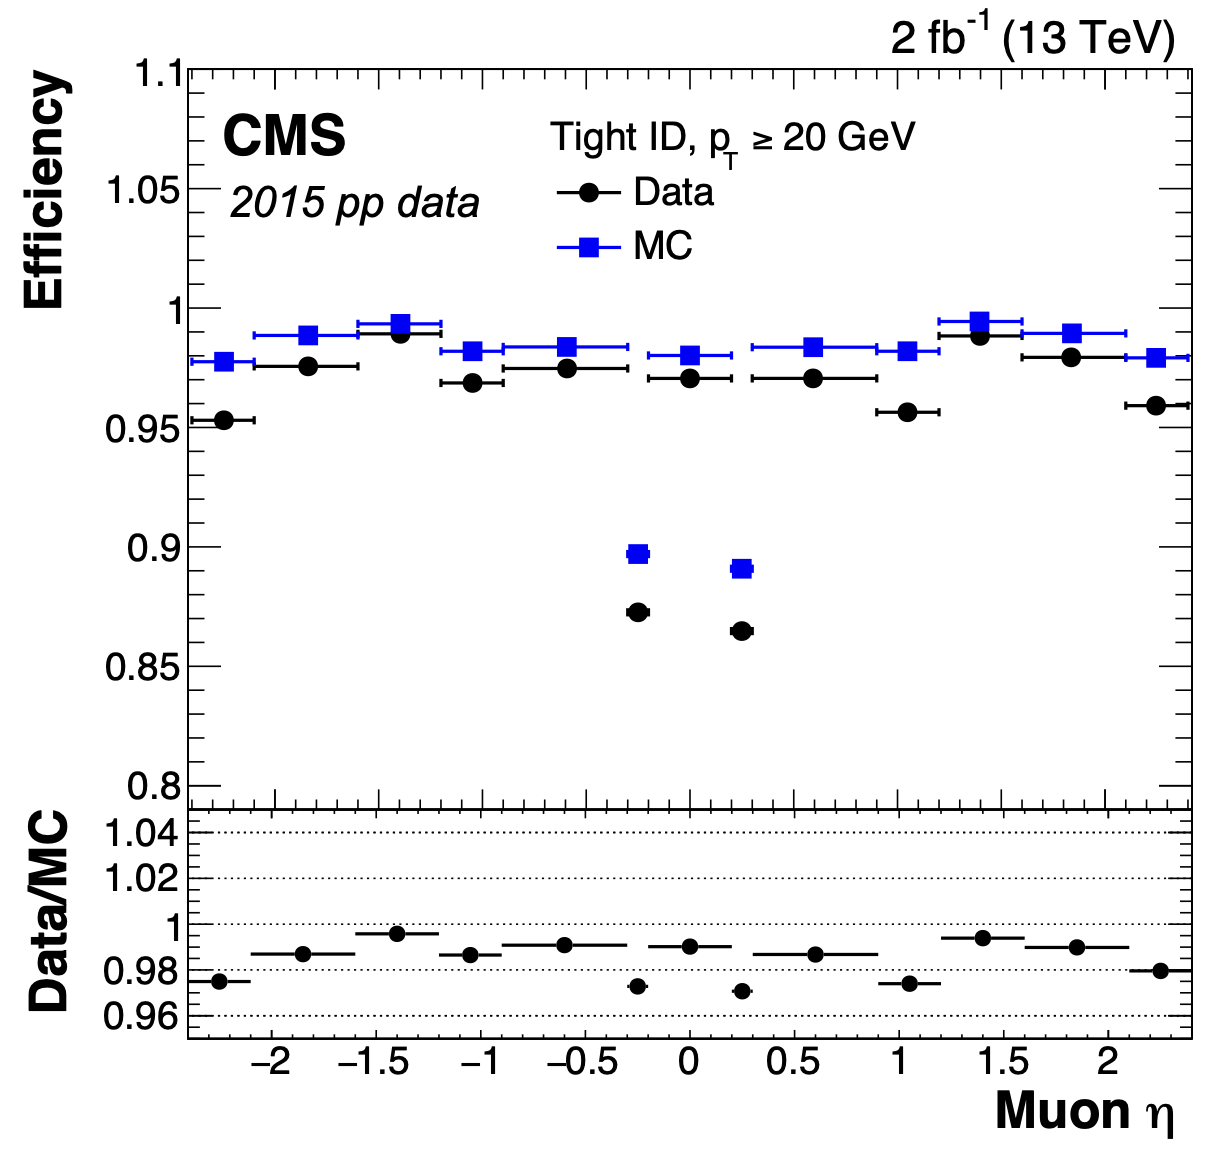
\includegraphics[width=1.0\textwidth]{figures/ch-5-object-reconstruction-and-corrections-applied/muon_efficiency_tightID}
        \caption{Muon isolation efficiency vs. $|\eta|$.}
        \label{fig:muon_tightID_efficiency}
    \end{subfigure}
    \caption[Muon identification efficiencies in 2015 data and MC as a function of the muon $p_{T}$ for the loose ID (\textit{left}) and tight ID (\textit{right}) working points.]{Muon identification efficiencies in 2015 data and MC as a function of the muon $p_{T}$ for the loose ID (\textit{left}) and tight ID (\textit{right}) working points \cite{CMS-MUO-16-001}.} 
\end{figure}

The efficiencies in data for the muon isolation, as measured in Level-3 muons (muons in one of the final stages of reconstruction in the HLT), as a function of the muon $p_{T}$ and $|\eta|$ are shown in Figures \ref{fig:muon_isolation_efficiency_vsPt} and \ref{fig:muon_isolation_efficiency_vsEta} \cite{CMS-MUO-16-001}. The HLT muon reconstruction consists of two steps: Level-2 (L2), where the muon is reconstructed in the muon subdetectors only, and Level-3 (L3) which is a global fit of tracker and muon hits (i.e. the global muon reconstruction as described in Section \ref{section:ch-5-muon-reconstruction}) \cite{Verwilligen-proceedings-2016}.

\begin{figure}[h]
    \centering
    \begin{subfigure}{0.45\textwidth}
        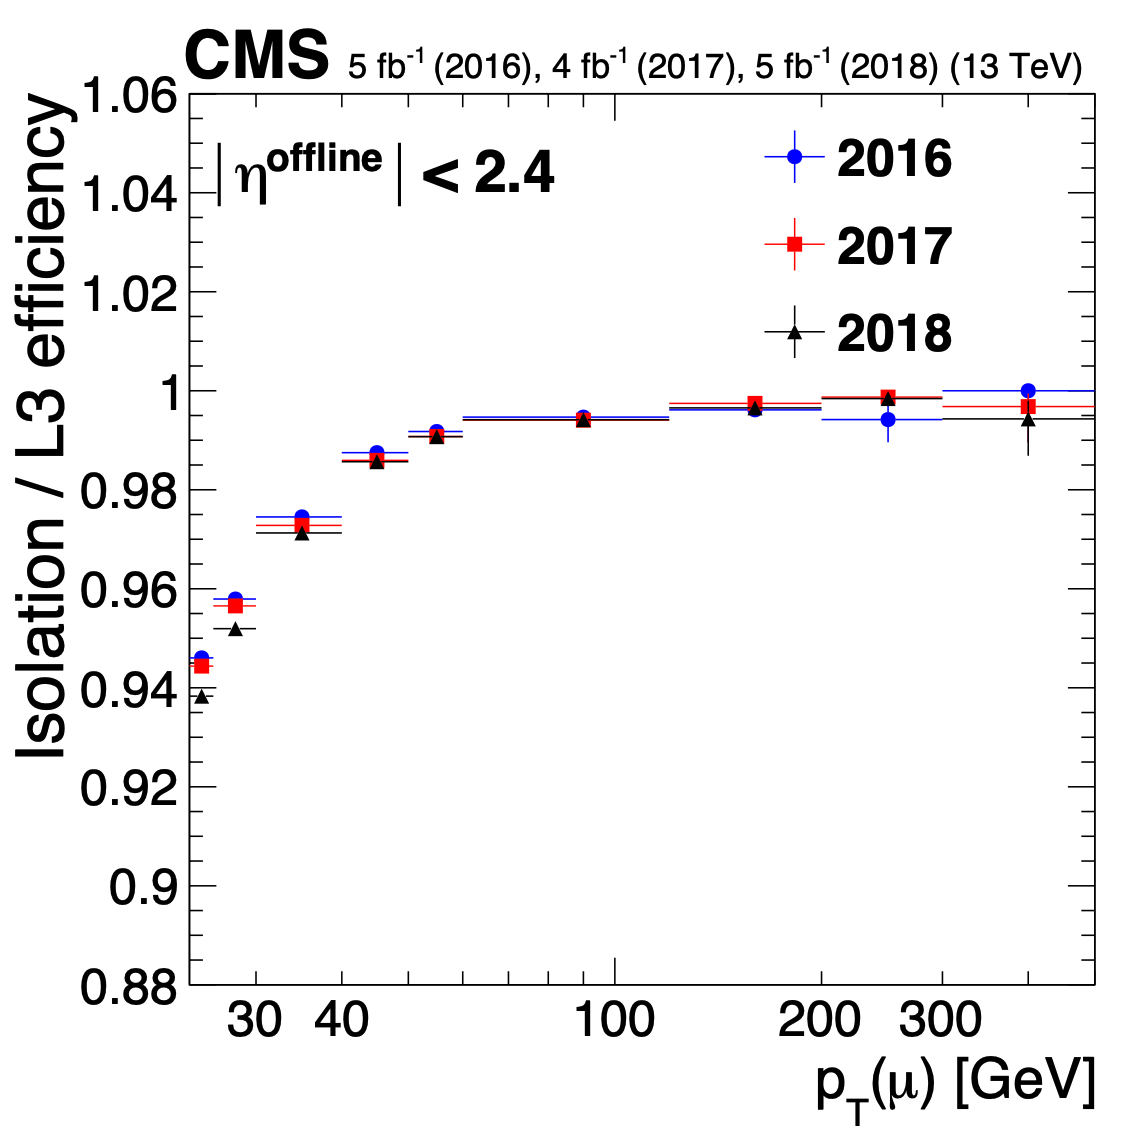
\includegraphics[width=1.0\textwidth]{figures/ch-5-object-reconstruction-and-corrections-applied/muon_efficiency_isolation_vsPt}
        \caption{Muon efficiency isolation vs $p_{T}$.}
        \label{fig:muon_isolation_efficiency_vsPt}
    \end{subfigure}
    \hfill
    \begin{subfigure}{0.45\textwidth}
        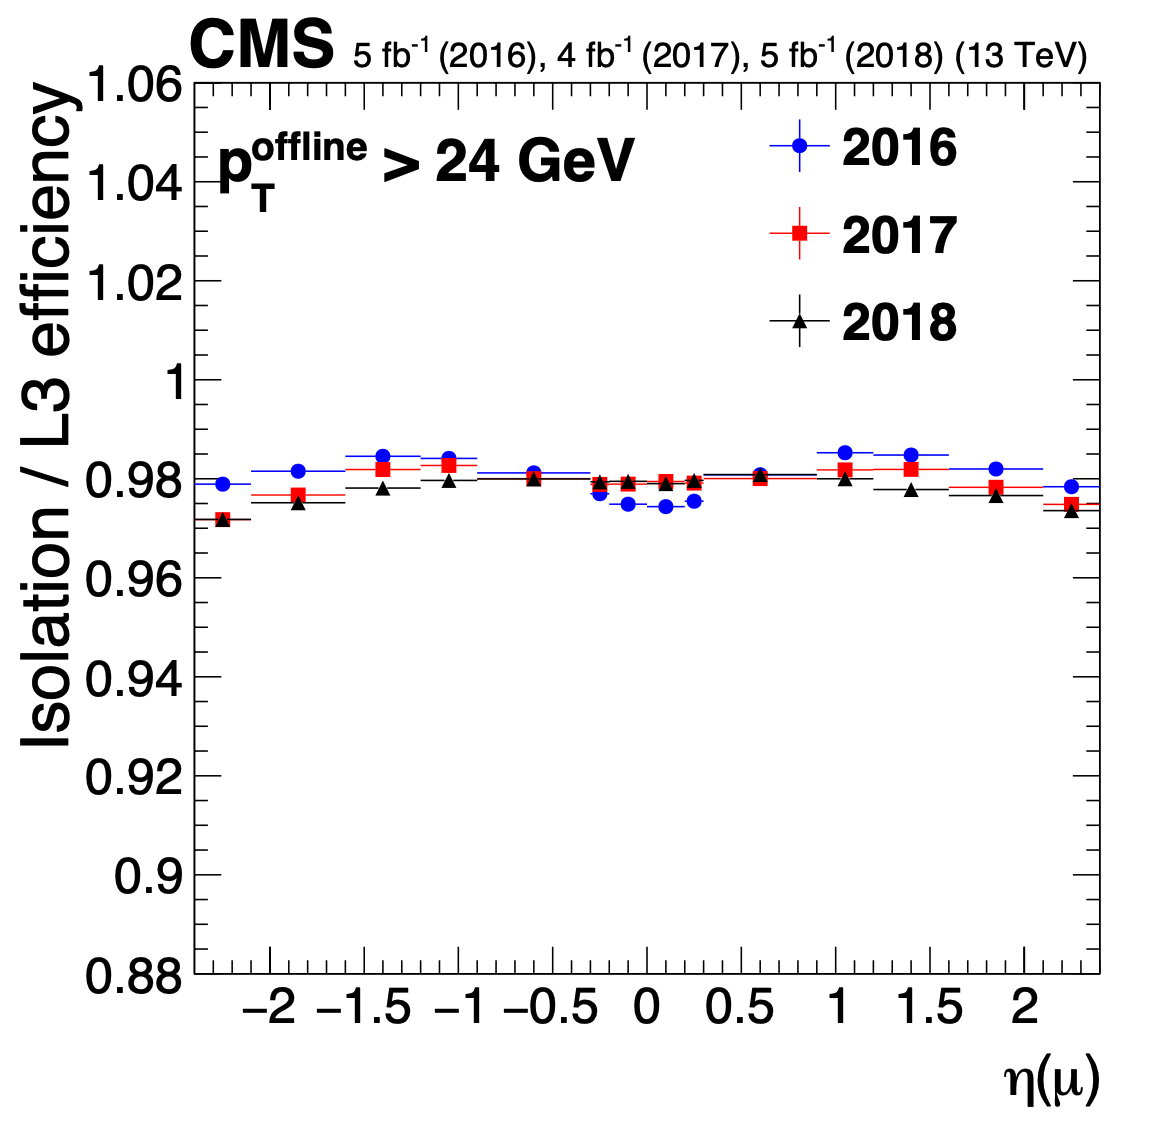
\includegraphics[width=1.0\textwidth]{figures/ch-5-object-reconstruction-and-corrections-applied/muon_efficiency_isolation_vsEta}
        \caption{Muon isolation efficiency vs. $|\eta|$.}
        \label{fig:muon_isolation_efficiency_vsEta}
    \end{subfigure}
    \caption[Muon isolation efficiencies in Run-2 data as a function of the muon $p_{T}$ (\textit{left}) and $|\eta|$ (\textit{right}).]{Muon isolation efficiencies in Run-2 data with respect to Level-3 muons (one of the final stages of HLT muon reconstruction) as a function of the muon $p_{T}$ (\textit{left}) and $|\eta|$ (\textit{right}) \cite{CMS-MUO-16-001}.} 
\end{figure}

The muon tracking efficiencies as a function of $|\eta|$ for standalone muons (i.e. tracks from only the muon system, i.e. DT, CSC, and RPC, as discussed in Section \ref{section:ch-5-muon-reconstruction}), is shown for data and simulated Drell-Yan samples in Fig. \ref{fig:muon_tracking_efficiency} \cite{CMS-DP-2020-035}. 

\begin{figure}[h]
    \centering
    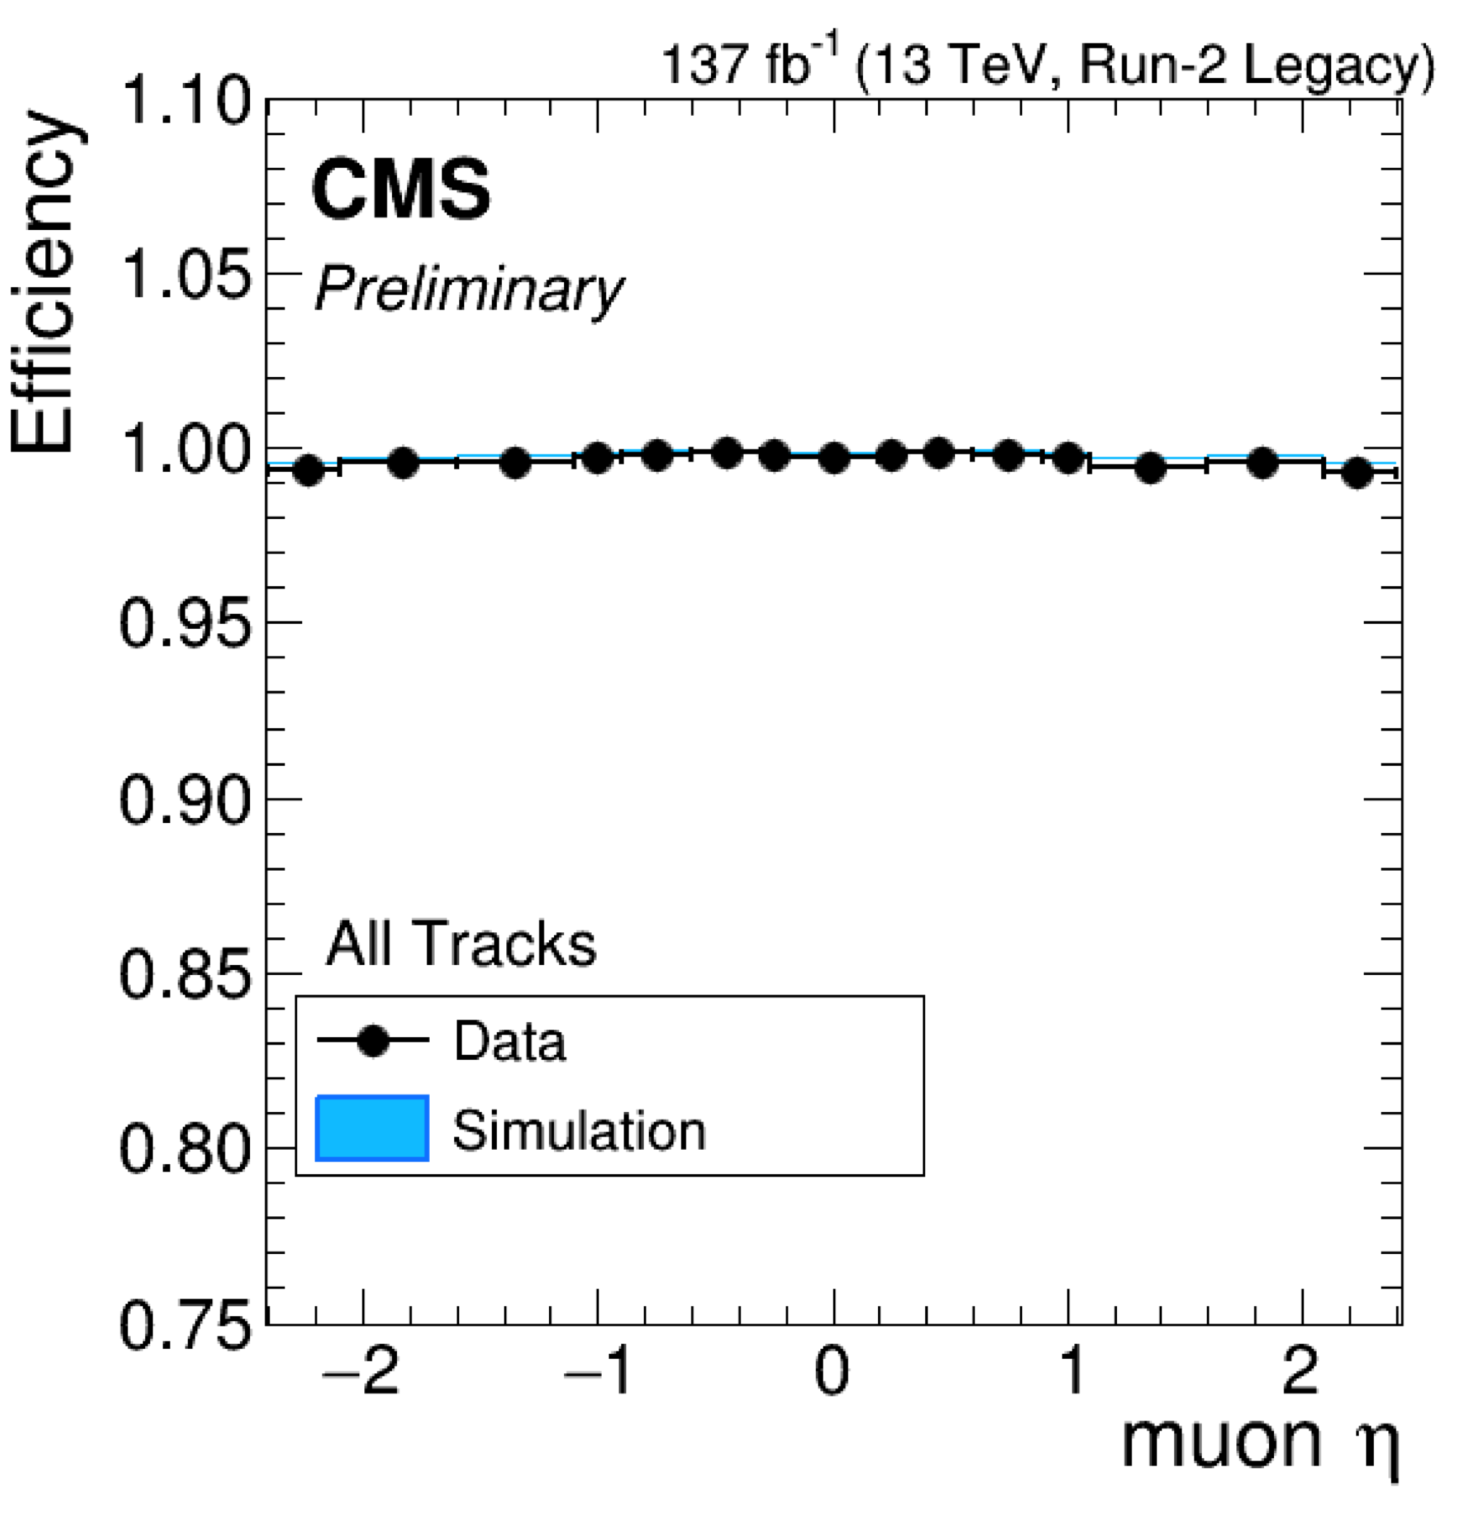
\includegraphics[width=8cm]{figures/ch-5-object-reconstruction-and-corrections-applied/muon_tracking_efficiency}
    \caption[Muon tracking efficiencies as a function of $|\eta|$ for standalone muons in Run-2 data (\textit{black}) and Drell-Yan (\textit{blue}) MC simulation.]{Muon tracking efficiencies as a function of $|\eta|$ for standalone muons in Run-2 data (\textit{black}) and Drell-Yan MC simulation (\textit{blue}) \cite{CMS-DP-2020-035}. All Tracks refers to tracks which exploit the presence of muon candidates in the muon system to seed the track reconstruction in the inner tracker, in contrast to tracks that use tracker-only hits for seeding. Uncertainties shown are statistical.}
    \label{fig:muon_tracking_efficiency}
\end{figure}

    

\subsection{Recoil corrections}
\label{sec:ch-8-recoil-corrections}
In proton-proton collisions, W and Z bosons are predominantly produced through quark-antiquark annihilation. Higher-order processes can induce radiated quarks or gluons that recoil against the boson, imparting a non-zero transverse momentum to the boson \cite{2009-Tevatron-recoil-correction}. Recoil corrections accounting for this effect are applied to samples with W+jets, Z+jets, and Higgs bosons \cite{twiki_HiggsToTauTauWorkingLegacyRun2}. The corrections are performed on the vectorial difference between the measured missing transverse momentum and the total transverse momentum of neutrinos originating from the decay of the W, Z, or Higgs boson. This vector is projected onto the axes parallel and orthogonal to the boson $p_{T}$. This vector, and the resulting correction to use, is measured in $Z \rightarrow \mu\mu$ events, since these events have leptonic recoil that do not contain neutrinos, allowing the 4-vector of the Z boson to be be measured precisely. The corrections are binned in generator-level $p_{T}$ of the parent boson and also the number of jets in the event.

\subsection{Drell-Yan corrections}
The Z boson transverse momentum distribution disagrees between leading-order (LO) simulations and data in a $Z \rightarrow \mu\mu$ control region with at least one b-tag jet \cite{CMS-HIG-17-024}. Per-event weights derived by the 2016 data-only version of this analysis \cite{CMS-HIG-17-024} are applied to $Z \rightarrow \tau\tau / \ell \ell$ events, as a function of the generator-level Z boson $p_{T}$ to provide better matching of MC to data.

\subsection{Pileup reweighing}
Reweighing is performed to rescale MC events to account for differences between MC and data, in the distribution of the pileup (number of additional proton-proton interactions per bunch crossing). A tool for calculating the pileup reweighing for the MC samples used is provided centrally by the Luminosity POG \cite{twiki_LUMI_POG_recommendation}.

\subsection{Pre-firing corrections}
In 2016 and 2017 data-taking, a gradual timing shift of ECAL was not properly propagated to L1 trigger primitives (TPs), resulting in a large fraction of high $\eta$ TPs being incorrectly associated with the previous bunch crossing. L1 trigger rules prevent two consecutive bunch crossings from firing, causing events to be rejected if significant ECAL energy was deposited in $2.0 < |\eta| 3.0$. To account for this issue, MC simulations for 2016 and 2017 are corrected using an event-dependent weight. Embedded samples are not corrected \cite{CMS-HIG-19-010}.

\subsection{Top \texorpdfstring{$p_{T}$}{pT} spectrum reweighing}
In Run-1 and Run-2 it was observed that the $p_{T}$ spectra of top quarks in $t\bar{t}$ data was significantly softer than those predicted by MC simulations \cite{twiki_Top_pt_reweighing}. Possible sources of this discrepancy are higher order QCD and/or electroweak corrections, and non-resonant production of $t\bar{t}$-like final states. To account for this, corrections derived from Run-2 data by the Top Physics Analysis Group (PAG) are applied to the $p_{T}$ of the top and anti-top quarks in MC simulations, computed as a function of their generator-level $p_{T}$ \cite{twiki_Top_pt_reweighing}.

\subsection{B-tagging efficiency}
In order to predict correct b-tagging discriminant distributions and event yields in data, the weight of selected MC events is reweighed according to recommendations by the BTV POG \cite{twiki_btag_SF_methods}. The reweighing depends on the jet $p_{T}$, $\eta$, and the b-tagging discriminant. In this method, there is no migration of events from one b-tag multiplicity bin to another.

\subsection{Jet energy resolution and jet energy smearing}
Calibration of jet energies, i.e. ensuring that the energy and momentum of the reconstructed jet matches that of the quark/gluon-initiated jet, is a challenging task due to time-dependent changes in the detector response and calibration and high pileup \cite{CMS-JME-13-004} \cite{proceedings-Agarwal:2022txa}. Jet calibration is done via jet energy corrections (JECs) applied to the $p_{T}$ of jets in MC samples, accounting successively for the effects of pileup, uniformity of the detector response, and residual data-simulation jet energy scale differences \cite{twiki_JetResolution_JEC}. Typical jet energy resolutions reported at $\sqrt{s} = 8$ TeV in the central rapidities are 15-20\% at 30 GeV and about 10\% at 100 GeV \cite{CMS-JME-13-004}. Jet energy corrections are also propagated to the missing transverse energy.

Measurements show that the jet energy resolution (JER) in data is worse than in simulation, and so the jets in MC need to be smeared to describe the data. JER corrections are applied after JEC on MC simulations, and adjust the width of the $p_{T}$ distribution based on pileup, jet size, and jet flavour \cite{twiki_JetResolution_JER}. Tools for applying JEC and JER are provided centrally by the JER Corrections group. 

\chapter{Event selection}
\section{General procedure for all channels}
For the search for $h \rightarrow aa \rightarrow bb\tau\tau$, three final states of the $\tau\tau$ system are considered: $\mu\tau_{h}$, $e\tau_{h}$, and $e\mu$. The $\tau_{h}\tau_{h}$ final state is not considered because signal events in the $\tau_{h}\tau_{h}$ channel would typically produce hadronic taus with momenta below data-taking trigger thresholds.

In all three final states, events are required to have at least one b-tag jet passing the medium working point of the DeepFlavour tagger, with $p_{T} > 20$ GeV, and $|\eta| < 2.4$. A second b-tag jet is not required because such a requirement would reduce signal acceptance by 80\% compared to only requiring one b-tag jet.


Events in MC samples are sorted into one of the three $\tau\tau$ channels if they pass the following trigger requirements and requirements on the offline reconstructed objects in the event, first checking the HLT paths for the $\mu\tau_{h}$ channel, then $e\tau_{h}$, and finally $e\mu$. The two leading leptons (e.g. muon and hadronic tau for the $\mu\tau_{h}$ channel) that were determined to have originated from the $\tau\tau$ decay, are called the $\tau\tau$ ``legs'' and are respectively subscripted $1$ and $2$ in this work. For events in data and embedded samples, the HLT paths requirements for the corresponding channel are checked.

After sorting events by HLT paths and identifying the leading tau legs in the offline reconstructed objects, the $p_{T}$ of the offline objects is checked against the online trigger thresholds. Trigger matching is also performed, which checks the correspondence between each offline reconstructed object used in the analysis (e.g. a muon), and a trigger object in the HLT (e.g. a HLT muon). An offline object is considered to be matched, if it corresponds to a trigger object of the same object type, with $\Delta R < 0.5$. This matched trigger object is also required to pass the filter(s) of the HLT trigger.

Further cuts are made on the offline objects in each channel to obtain the signal region, or other data regions used to perform data-driven background estimations. These are detailed below. 

\section{Event selection in the \texorpdfstring{$\mu\tau_{h}$}{mutauh} channel}
\label{section:ch-6-event-selection-mutau}
In all three years, a single muon trigger is used if the muon has sufficiently high $p_{T}$, otherwise a dilepton $\mu\tau_{h}$ cross-trigger is used (Tables \ref{table:trigger2016}, \ref{table:trigger2017}, and \ref{table:trigger2018}). For data taken in 2017-2018 (2016), the logical OR of the single muon triggers with online $p_{T}$ thresholds 24 and 27 (23) GeV is used, with the corresponding offline muon required to have with $p_{T}$ 1 GeV above the online threshold. For data taken in 2017-2018 (2016), a dilepton $\mu + \tau_{h}$ cross-trigger with $p_{T}$ thresholds of 20 (19) and 27 (20) GeV for the muon and tau respectively, is used. The $\tau_{h}$ is required to have $|\eta| < 2.3$ if the single trigger is fired, $|\eta| < 2.1$. 

The muon and $\tau_h$ are required to have opposite charge and be separated by $\Delta R > 0.4$. The muon is required to have $|\eta| < 2.4$, and the $\tau_{h}$ is required to have $|\eta| < 2.3$ unless a cross-trigger is required, in which case we require $|\eta| < 2.1$ as discussed above.

The muon is required to pass the medium identification (ID) working point \cite{twiki_MUON_POG_Run2_guide}, which is defined by the Muon POG as a loose muon (i.e. a Particle Flow muon that is either a global or a tracker muon - see Section \ref{section:ch-5-muon-reconstruction}) with additional requirements on track quality and muon quality. This identification criteria is designed to be highly efficiently for prompt muons and for muons from heavy quark decays. In addition to the ID, for prompt muons it is recommended to apply cuts on the impact parameter \cite{twiki_MUON_POG_Run2_guide}: we apply $|\Delta(z)| < 0.2$ and $|\Delta(xy)| < 0.045$. 

In addition, a cut is applied on the muon relative isolation (defined in Section \ref{section:ch-5-muon-reconstruction}), to be less than 0.15 in a cone size of $\Delta R = 0.4$, which corresponds to the Tight Particle Flow isolation requirement \cite{twiki_MUON_POG_Run2_guide}.

The $\tau_h$ is required to pass a cut on its impact parameter of $|\Delta(z)| < 0.2$. The $\tau_h$ is also required to pass the VLoose (Very Loose) DeepTau working point vs. electron, the Tight DeepTau working point vs. muons, and the VVVLoose and Medium DeepTau working point vs. jets. Events with taus reconstructed in two of the decay modes (labeled 5 and 6) are rejected, since these decay modes are meant to recover 3-prong taus, but are only recommended for use in analyses where the benefits in final significance outweigh the resulting increase in background \cite{twiki_TAU_POG_tauidrecommendationforrun2}.

For the estimation of the background from jets faking $\tau_{h}$, which is described in Section \ref{section:ch-7-jet-faking-tauh-background}, anti-isolated events are selected, by requiring events to pass all the selections described above, except failing the Medium DeepTau working point vs. jets.

\section{Event selection in the \texorpdfstring{$e\tau_{h}$}{etauh} channel}
\label{section:ch-6-event-selection-etau}

The HLT trigger paths for the $e\tau_{h}$ channel are summarized in Tables \ref{table:trigger2016}, \ref{table:trigger2017}, and \ref{table:trigger2018}. Similarly to the $\mu\tau_{h}$ channel, a single electron trigger is used if the electron has sufficiently high $p_{T}$ in 2018 and 2017. For data taken in 2018 (2017), the OR of the single electron triggers with online $p_{T}$ thresholds at 32 and 35 (27 and 32) GeV are used, with the corresponding offline electrons required to have $p_{T}$ greater than 33 (28) GeV. A $e + \tau_{h}$ cross-trigger is used for electrons with lower offline $p_{T}$ between 25 and 33 GeV (25 and 28 GeV). For the 2016 dataset, there is no cross trigger but only a single electron trigger with online $p_{T}$ threshold at 25 GeV, which is used if the offline electron has $p_{T}$ greater than 26 GeV.

The electron and $\tau_h$ are required to have opposite charge and be separated by $\Delta R > 0.4$. The electron is required to be within $|\eta| < 2.3$ when no cross trigger is used, and $|\eta| < 2.1$ when the cross trigger is fired. The $\tau_{h}$ is required to have $|\eta| < 2.3$ if no cross trigger is fired, and have $|\eta| < 2.1$ if the cross trigger is fired.

The electron is required to have a relative isolation (same definition as in Section \ref{section:ch-5-muon-reconstruction}) of less than 0.1 in a cone size of $\Delta R = 0.3$, which is the standard recommended cone size giving minimal pileup dependence and reduced probability of other objects overlapping with the cone. The isolation quantity used includes an ``effective area'' (EA) correction to remove the effect of pileup in the barrel and endcap parts of the detector \cite{twiki_EGamma_cutbased_ID_info}.

The electron is also required to pass cuts on its impact parameter of $|\Delta(z)| < 0.2$ and $|\Delta(xy)| < 0.045$. It is also required to pass the non-isolated MVA working point corresponding to 90\% efficiency. The electron's number of missing hits, which are gaps in its trajectory through the inner tracker \cite{twiki_EGamma_cutbased_ID_info}, must be less than or equal to 1. The electron must pass a conversion veto, which rejects electrons coming from photon conversions in the tracker, which should instead be reconstructed as part of the photon \cite{twiki_EGamma_cutbased_ID_info}.

The impact parameter cut for the $\tau_h$ is  $|\Delta(z)| < 0.2$. In contrast to the $\mu\tau_{h}$ event selection, the vs. electron and vs. muon DeepTau working points are flipped, to reject muons faking the $\tau_{h}$ leg. The $\tau_h$ is required to pass the Tight DeepTau working point vs. electrons, the VLoose DeepTau working point vs. muons, and the Medium DeepTau working point vs. jets.

As in the $\mu\tau_{h}$ channel, for the estimation of the background from jets faking $\tau_{h}$, which is described in Section \ref{section:ch-7-jet-faking-tauh-background}, anti-isolated events are selected, by requiring events to pass all the selections described above, except failing the Medium DeepTau working point vs. jets.

\section{Event selection in the \texorpdfstring{$e\mu$}{emu} channel}
\label{section:ch-6-event-selection-emu}

The HLT trigger paths for the $e\mu$ channel are summarized in Tables \ref{table:trigger2016}, \ref{table:trigger2017}, and \ref{table:trigger2018}. Events are selected with the logical OR of two $e+\mu$ cross triggers, where either the electron or muon can have larger $p_{T}$: (1) leading electron, where the electron has online $p_{T} > 23$ GeV and muon has online $p_{T} > 8$ GeV, or (2) leading muon, where electron has online $p_{T} > 12$ GeV and muon has online $p_{T}>23$ GeV.

The leading and sub-leading leptons are required to have an offline $p_{T}$ greater than 1 GeV above the online threshold (i.e. $p_{T} > 24$ GeV). If the sub-leading lepton is the electron, the offline $p_{T}$ threshold is 1 GeV above the online threshold ($p_{T} > 13$ GeV), but if it is a muon, the offline $p_{T}$ threshold is required to be at least 5 GeV greater than the online threshold (i.e. $p_T > 13$ GeV). This is because of poor data and simulation agreement for low-$p_T$ muons with $p_T$ between 9 GeV and 13 GeV, and the higher probability of mis-identifying jets as muons at lower $p_{T}$. With no effect on the expected limits, the offline $p_{T}$ threshold for muons is raised to 13 GeV instead of 9 GeV, even though it may lead to loss in signal acceptance. Both the electron and muon are required to be have $|\eta| < 2.4$.

The electron and muon are required to have opposite charge and be separated by $\Delta R > 0.3$ (note the decreased separation requirement compared to the other two channels). The electron is required to pass the non-isolated MVA identification working point corresponding to 90\% efficiency, and to have a relative isolation less than 0.1 for a cone size of $\Delta R = 0.3$ with the EA pileup subtraction correction. The electron must have one or fewer missing hits and pass the conversion veto (both described previously in Section \ref{section:ch-6-event-selection-etau}). 

The muon is required to pass the medium identification working point (described earlier in \ref{section:ch-6-event-selection-mutau}), and to have a relative isolation less than 0.15 for a cone size of $\Delta R = 0.4$. The muon impact parameter is required to have $|\Delta(z)| > 0.2$ and $|\Delta(xy) < 0.045$. 

For the QCD multijet background estimation described in Section \ref{section:ch-7-QCD-multijet-background}, the same-sign region is selected by requiring all the above selections, except the legs are required to have the same electric charge rather than opposite.


\begin{table}[]
    \centering
    \begin{tabular}{ll}
    \hline
    \multicolumn{2}{|c|}{\footnotesize{2016 $\mu\tau_{h}$ trigger paths}}                                     \\ \hline
    \footnotesize{Notes}          & \footnotesize{HLT Path}                                           \\ \hline
                                  & \footnotesize{HLT\_IsoMu22\_v}                                    \\
                                  & \footnotesize{HLT\_IsoMu22\_eta2p1\_v}                            \\
                                  & \footnotesize{HLT\_IsoTkMu22\_v}                                  \\
                                  & \footnotesize{HLT\_IsoTkMu22\_eta2p1\_v}                          \\
                                  & \footnotesize{HLT\_IsoMu19\_eta2p1\_LooseIsoPFTau20\_v}           \\
                                  & \footnotesize{HLT\_IsoMu19\_eta2p1\_LooseIsoPFTau20\_SingleL1\_v} \\ \hline
    \multicolumn{2}{|c|}{\footnotesize{2016  $e\tau_{h}$ trigger paths}}                                         \\ \hline
    \footnotesize{Notes}          & \footnotesize{HLT Path}                                           \\ \hline
                                  & \footnotesize{HLT\_Ele25\_eta2p1\_WPTight\_Gsf\_v}                \\ \hline
    \multicolumn{2}{|c|}{\footnotesize{2016 $e\mu$ trigger paths}}                                            \\ \hline
    \footnotesize{Notes}           & \footnotesize{HLT Path}                                                     \\ \hline
    \footnotesize{runs B-F and MC} & \footnotesize{HLT\_Mu23\_TrkIsoVVL\_Ele12\_CaloIdL\_TrackIdL\_IsoVL\_v}     \\
    \footnotesize{runs B-F and MC} & \footnotesize{HLT\_Mu8\_TrkIsoVVL\_Ele23\_CaloIdL\_TrackIdL\_IsoVL\_v}      \\
    \footnotesize{runs G-H}        & \footnotesize{HLT\_Mu23\_TrkIsoVVL\_Ele12\_CaloIdL\_TrackIdL\_IsoVL\_DZ\_v} \\
    \footnotesize{runs G-H}        & \footnotesize{HLT\_Mu8\_TrkIsoVVL\_Ele23\_CaloIdL\_TrackIdL\_IsoVL\_DZ\_v} 
    \end{tabular}
    \caption{High-Level Trigger (HLT) paths used to select data and simulation events in 2016 for the three $\tau\tau$ channels.}
    \label{table:trigger2016}
\end{table}

    
\begin{table}[]
    \centering
    \begin{tabular}{ll}
    \hline  
    \multicolumn{2}{|c|}{\footnotesize{2017 $\mu\tau_{h}$ trigger paths}}                                     \\ \hline
    \footnotesize{Notes}         & \footnotesize{HLT Path}                                                           \\ \hline
                                 & \footnotesize{HLT\_IsoMu24\_v}                                                    \\
                                 & \footnotesize{HLT\_IsoMu27\_v}                                                    \\
                                 & \footnotesize{HLT\_IsoMu20\_eta2p1\_LooseChargedIso\_PFTau27\_eta2p1\_CrossL1\_v} \\ \hline
    \multicolumn{2}{|c|}{\footnotesize{2017  $e\tau_{h}$ trigger paths}}                                         \\ \hline
    \footnotesize{Notes}         & \footnotesize{HLT Path}                                                       \\ \hline
                                 & \footnotesize{HLT\_Ele32\_WPTight\_Gsf\_v}                                                    \\
                                 & \footnotesize{HLT\_Ele35\_WPTight\_Gsf\_v}                                                    \\
                                 & \footnotesize{HLT\_Ele24\_eta2p1\_WPTight\_Gsf\_Loose\_ChargedIsoPFTau30\_eta2p1\_CrossL1\_v} \\ \hline
    \multicolumn{2}{|c|}{\footnotesize{2017 $e\mu$ trigger paths}}                                            \\ \hline
    \footnotesize{Notes}         & \footnotesize{HLT Path}                                                        \\ \hline
                                 & \footnotesize{HLT\_Mu23\_TrkIsoVVL\_Ele12\_CaloIdL\_TrackIdL\_IsoVL\_DZ\_v}    \\
                                 & \footnotesize{HLT\_Mu8\_TrkIsoVVL\_Ele23\_CaloIdL\_TrackIdL\_IsoVL\_DZ\_v}                   
    \end{tabular}
    \caption{High-Level Trigger (HLT) paths used to select data and simulation events in 2017 for the three $\tau\tau$ channels.}
    \label{table:trigger2017}
\end{table}
    
    

\begin{table}[]
    \centering
    \begin{tabular}{ll}
    \hline
    \multicolumn{2}{|c|}{\footnotesize{2018 $\mu\tau_{h}$ trigger paths}}                                     \\ \hline
    \footnotesize{Notes}          & \footnotesize{HLT Path}                                                   \\ \hline
                                  & \footnotesize{HLT\_IsoMu24\_v}                                                           \\
                                  & \footnotesize{HLT\_IsoMu27\_v}                                                           \\
    \footnotesize{only data run $<$ 317509}      & \footnotesize{HLT\_IsoMu20\_eta2p1\_ (contd.)} \\
                                                 & \footnotesize{LooseChargedIsoPFTauHPS27\_eta2p1\_CrossL1\_v} \\
    \footnotesize{MC and data run $\geq$ 317509} & \footnotesize{HLT\_IsoMu20\_eta2p1\_ (contd.)} \\
                                                 & \footnotesize{LooseChargedIsoPFTauHPS27\_eta2p1\_TightID\_CrossL1\_v}     \\ \hline
    \multicolumn{2}{|c|}{\footnotesize{2018 $e\tau_{h}$ trigger paths}}                                       \\ \hline
    \footnotesize{Notes}          & \footnotesize{HLT Path}                                                   \\ \hline
                                  & \footnotesize{HLT\_Ele32\_WPTight\_Gsf\_v}                                               \\
                                  & \footnotesize{HLT\_Ele35\_WPTight\_Gsf\_v}                                               \\
    \footnotesize{only data run $<$ 317509}      & \footnotesize{HLT\_Ele24\_eta2p1\_WPTight\_Gsf\_ (contd.)} \\
                                                 & \footnotesize{LooseChargedIsoPFTauHPS30\_eta2p1\_CrossL1\_v}          \\
    \footnotesize{MC and data run $\geq$ 317509} & \footnotesize{HLT\_Ele24\_eta2p1\_WPTight\_Gsf\_ (contd.)} \\
                                                 & \footnotesize{LooseChargedIsoPFTauHPS30\_eta2p1\_TightID\_CrossL1\_v} \\ \hline
    \multicolumn{2}{|c|}{\footnotesize{2018 $e\mu$ trigger paths}}                                            \\ \hline
    \footnotesize{Notes}          & \footnotesize{HLT Path}                                                   \\ \hline
                                  & \footnotesize{HLT\_Mu23\_TrkIsoVVL\_Ele12\_CaloIdL\_TrackIdL\_IsoVL\_DZ\_v}              \\
                                  & \footnotesize{HLT\_Mu8\_TrkIsoVVL\_Ele23\_CaloIdL\_TrackIdL\_IsoVL\_DZ\_v}                             
    \end{tabular}
    \caption{High-Level Trigger (HLT) paths used to select data and simulation events in 2018 for the three $\tau\tau$ channels. In 2018 a HLT trigger path using the hadron plus strips (HPS) tau reconstruction algorithm became available.}
    \label{table:trigger2018}
\end{table}


\section{Extra lepton vetoes in all channels}

Events containing a third lepton (electron or muon) that is neither of the leading $\tau\tau$ legs are rejected, and events with di-muons and di-electrons are vetoed, with criteria taken from the Standard Model $H \rightarrow \tau\tau$ working group \cite{twiki_HiggsToTauTauWorkingLegacyRun2}.

The event is vetoed if a third electron is found with the following properties: $p_{T} > 10$ GeV, $|\eta| < 2.5$, impact parameter $|\Delta(z)| < 0.2$ and $|\Delta(xy)| < 0.045$, passing non-isolation MVA identification with 90\% efficiency, conversion veto, $\leq 1$ missing hits, and relative isolation $<0.3$ with cone size $\Delta R = 0.3$. The event is also vetoed if a third muon is found with the following properties: $p_{T} > 10$ GeV, $|\eta| < 2.4$, impact parameter $|\Delta(z)| < 0.2$ and $|\Delta(xy)| < 0.045$, medium ID, and isolation $<0.3$ with cone size $\Delta R = 0.4$. 

A di-muon veto is applied, which rejects events containing a pair of muons with opposite charge and separation of $\Delta R > 0.15$, that both pass the following selections: $p_T > 15$ GeV, $|\eta| < 2.4$, flag for global muons, flag for tracker muon, flag for Particle Flow muon, $|\Delta(z)| < 0.2$, $|\Delta(xy)| < 0.045$, and isolation $<0.3$ with cone size $\Delta R = 0.4$.

A similar di-electron veto is applied to reject events containing a pair of electrons with opposite charge and separation of $\Delta R > 0.15$, that both pass the following selections: $p_T > 15$ GeV, $|\eta| < 2.5$, a dedicated electron ID (cut-based) for vetoing third leptons, $|\Delta(z)| < 0.2$, $|\Delta(xy)| < 0.045$, with pileup-corrected relative isolation $<0.3$ with cone size $\Delta R = 0.3$. 

These vetoes on extra leptons also ensure orthogonality of events to analyses such as the $bb\mu\mu$ final state, whose results are combined with this $bb\tau\tau$ final state as described in Section \ref{section:ch-13-combination-procedure-with-bbmumu}.

\chapter{Background estimation}
\label{chapter:ch-7:background-estimation}
This section describes methods used to estimate backgrounds from Standard Model processes in the search for $h \rightarrow aa \rightarrow bb\tau\tau$. The background contributions directly taken from MC are described in Sections \ref{section:background-estimation:z-plus-jets} to \ref{section:background-estimation:SM-higgs}. Section \ref{section:ch-7-jet-faking-tauh-background} describes the data-driven method for estimating backgrounds from jets faking hadronic tau decays (jet $\rightarrow \tau_{h}$), which is used in the $\mu\tau_{h}$ and $e\tau_{h}$ channels. Section \ref{section:ch-7-QCD-multijet-background} describes the data-driven method for estimating background from quantum chromodynamic (QCD) processes in the $e\mu$ channel.

\section{Z+jets}
\label{section:background-estimation:z-plus-jets}
A major source of background for $\tau\tau$ analyses is the Drell-Yan (DY) process (Z+jets). The Z boson decays to $\tau\tau/ \mu\mu/ ee$ with equal probability of 3.4\% each, with the dominant decay modes being to hadrons (around 70\%) and neutrinos (invisible) (20\%)~\cite{workman_review_2022}. 

The Drell-Yan contribution with genuine taus, Z $\rightarrow \tau\tau$, is estimated using embedded samples, described in Section \ref{section:embedded-samples}. To avoid double-counting between embedded and MC samples, in all MC samples, events with legs that originated from genuine $\tau$ are discarded.

The other decays of the Z, Z $\rightarrow ee$ and Z $\rightarrow \mu\mu$, are estimated from MC simulation, and are hereafter referred to as simply the Drell-Yan background. These MC samples are generated to leading order (LO) with different numbers of jets (jet multiplicity) in the matrix element: Z+1 jet, Z+2jets, Z+3 jets, Z+4 jets, and inclusive Z+jets. The cross-sections of the samples with $\geq 1$ jets are normalized to next-to-NLO (NNLO) in QCD. For the inclusive Drell-Yan sample, two samples are used with different thresholds for the di-lepton invariant mass ($m_{\ell}$) at the generator level: one with $m_{\ell\ell} > 50$ GeV and the other with $10 < m_{\ell\ell} < 50$. 

\section{W+jets}

The dominant W boson decay modes are to hadrons (67.4\%), $e + \nu_e$ (10.7\%), $\mu + \nu_\mu$ (10.6\%), and $\tau + \nu_\tau$ (11.4\%)~\cite{workman_review_2022}.
The W+jets background is estimated from MC simulation. Similarly to the Z+jets, the W+jets samples are generated with different jet multiplicities in the matrix element. LO samples are used for greater statistics and are normalized to NNLO cross sections. 

\section{\texorpdfstring{$t\bar{t}$}{ttbar} + jets}
In hadron collisions, top quarks are produced singly with the weak interaction, or in pairs via the strong interaction, with interference between these leading-order processes possible in higher orders of the perturbation theory. 
The top quark is the heaviest fermion in the Standard Model and has a short lifetime ($\sim 10^{-25}$ s), decaying without hadronization into a bottom quark and a W boson~\cite{workman_review_2022}, with the decay modes of the W boson as listed in the previous section. With two top quarks, the final states of the two resulting W bosons can be described as fully leptonic, semileptonic, and fully hadronic. These three final states are modeled separately with MC simulation in 2018 and 2017, while for 2016 the sample used is inclusive.

\section{Single top}
% https://cms.cern/news/measurement-t-channel-single-top-quark-production-rates-pp-collisions-7-tev
There are three main production modes of the single top in $pp$ collisions~\cite{CMS-CR-2018-185}: the exchange of a virtual W boson ($t$ channel), the production and decay of a virtual W boson ($s$ channel), and the associated production of a top quark and W boson ($tW$, or W-associated) channel. As the $s$ channel process is rare and only 3\% of the total production, the dominant production mode of the $t-channel$ and the $tW$ production are considered and modeled with MC. 

\section{Diboson}

In $pp$ collisions, the production of dibosons (pairs of electroweak gauge bosons, i.e. WW, WZ, and ZZ) is dominated by quark-antiquark annihilation, with a small contribution from gluon-gluon interactions~\cite{CMS-SMP-20-012}. MC is used to model the pair production and decays of VV to $2\ell 2\nu$, WZ to $2q 2\ell$ and $3 \ell \nu$, and ZZ to $4\ell$ and $2q 2\ell$ ($q$ being quarks and $\ell$ being leptons).

\section{Standard Model Higgs}
\label{section:background-estimation:SM-higgs}
MC is used to simulate backgrounds from major production modes of the Standard Model 125\GeV Higgs boson: gluon-gluon fusion (ggH), vector boson fusion (VBF), associated production with a W or Z (WH, ZH), and associated production with a top pair (ttH) (see Fig. \ref{fig:higgs-boson-production-modes} for leading-order diagrams). For these production modes, samples with the Higgs decaying to $\tau\tau$ or to $WW$ are used. Samples made with higher-order diagrams for WH and ZH that include the production of a jet, with the Higgs decaying to WW, are also used.

\begin{figure}[ht]
    \centering
    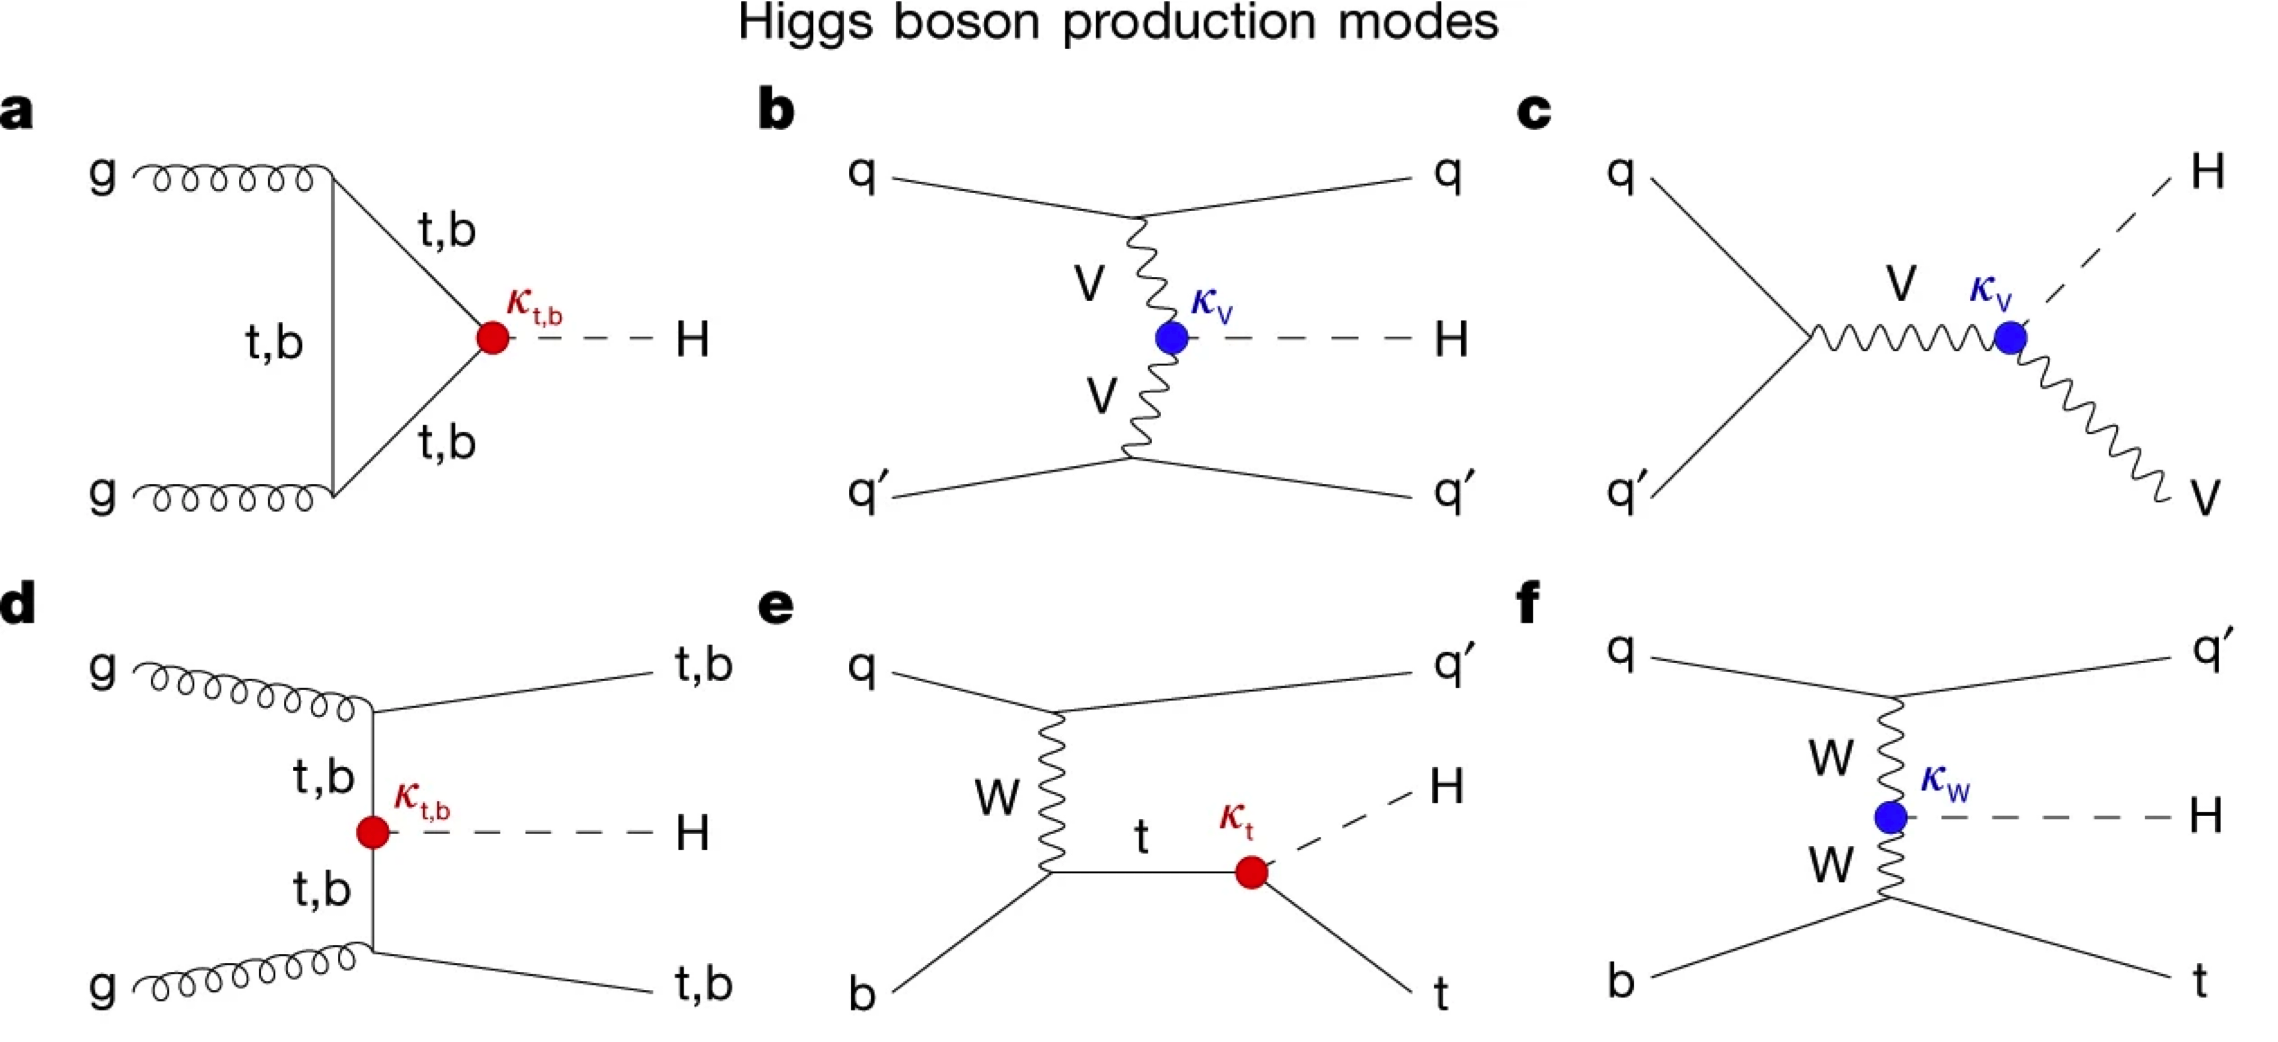
\includegraphics[width=15cm]{figures/ch-7-background-estimation/higgs-boson-production-modes.png}
    \caption[Leading-order Feynman diagrams of Higgs production.]{Leading-order Feynman diagrams of Higgs production from~\cite{CMS-HIG-22-001}, in ggH (\textit{a}) and vector boson fusion (VBF; \textit{b}), associated production with a W or Z (V) boson (VH; \textit{c}), associated production with a top or bottom quark pair (ttH or bbH); \textit{d}, and associated production with a single top quark (tH; \textit{e, f}).} 

     \label{fig:higgs-boson-production-modes}
\end{figure}

\section{Jet faking \texorpdfstring{$\tau_{h}$}{tauh}}
\label{section:ch-7-jet-faking-tauh-background}
Events with a jet mis-reconstructed as the hadronic tau leg $\tau_{h}$ are a major source of background in the $\mu\tau_{h}$ and $e\tau_{h}$ channels. The main processes contributing to jet $\rightarrow \tau_{h}$ events are QCD multijet, W+jets, and $t\bar{t}$ production. These events are estimated using a data-driven method adapted from past analyses~\cite{CMS-HIG-19-010}~\cite{CMS-HIG-17-024}. This background includes contributions from W+jets, QCD multijets, and $t\bar{t}$+jets. To estimate this background, a sideband region is constructed, where events are required to pass all baseline $\mu\tau_{h}/ e\tau_{h}$ selection criteria, but fail the $\tau_{h}$ isolation criteria. The events in this sideband region is reweighed with a factor $f/(1-f)$, where $f$ is the probability for a jet to be misidentified as a $\tau_{h}$. The jet $\rightarrow \tau_{h}$ background is the anti-isolated, reweighed MC and embedded events subtracted from the anti-isolated, reweighted data events.

The fake factor is measured in $Z \rightarrow \mu\mu$+jets events in data in the $\mu\mu\tau_{h}$ final state, as any reconstructed $\tau_{h}$ in these events must originate from a jet. The two muons are required to be isolated $(<0.15)$, have opposite electric charge, and have an invariant mass between 76 and 106 GeV (close to the Z mass). These events are selected with a double muon trigger, with the leading muon having offline $p_T > 20$ GeV and the subleading muon $p_{T} > 10$ GeV. Simulated diboson (ZZ and WZ) events are subtracted to avoid contamination from events with real $\tau_{h}$. The denominator of the fake rate corresponds to fake taus passing the VVVLoose working point of the discriminator vs. jets, while the numerator corresponds to those passing the Medium working point, i.e. $f = N_{\text{jet passing tight}}/ N_{\text{jet passing loose}}$.

$f$ is measured as a function of the $\tau_{h}$ transverse momentum and is 8\% - 10\% in each of the data-taking years. $f$ is derived separately for the $\mu\tau_{h}$ and $e\tau_{h}$ channels because the channels use different anti-lepton identification working points.

\section{QCD multijet background}
\label{section:ch-7-QCD-multijet-background}
In the $e\mu$ channel, the rate of events with jets faking electrons or muons originating from QCD multijet processes, is estimated from data events with the same baseline selection as in the signal region, except with same-signed (SS) charged $e+\mu$, ensuring orthogonality with the signal region which requires opposite-sign (OS) $e\mu$ pairs. All same-sign MC events (both events with real and fake $e+\mu$) are subtracted from same-sign data events to remove contamination from other backgrounds. i.e. QCD$_{\text{SS}}$ = Data$_{\text{SS}}$ - MC$_{\text{SS}}$.

Three scale factors are applied to the QCD$_{\text{SS}}$ events to compute the QCD multijet background~\cite{CMS-HIG-17-024}~\cite{CMS-HIG-22-007}:
\begin{itemize}
    \item \textit{OS-to-SS scale factor}: This scales the SS QCD to the OS region, and is measured from an orthogonal region with an isolated electron and an anti-isolated muon. Only the muon is chosen to be anti-isolated because this scale factor was observed to depend more strongly on electron isolation than on muon isolation. This scale factor is treated as a function of the $\Delta R$ separation of the trajectories of the electron and muon, and is measured separately for events with 0 jets, 1, jet, and greater than 1 jet.
    \item \textit{2D closure correction for the lepton $p_{T}$}: This factor accounts for subleading dependencies of the first scale factor on the $p_{T}$ of the two leptons. A 2D weight is derived in a similar fashion, as a ratio of QCD$_{OS}$ events to QCD$_{\text{SS}}$ events, but parameterized by both electron and muon $p_{T}$, where the SS events have the previous scale factor applied.
    \item \textit{Isolation correction for the muon}: The third and final factor is an isolation correction, which is a bias correction to account for the fact that the fake factor was determined for less-isolated muons. This factor is obtained as the ratio of the OS-to-SS scale factors measured in two other control regions: (1) events where the electron is anti-isolated ($0.15 <$ iso $< 0.5$) and the muon is isolated, and (2) events where both leptons are anti-isolated. 
\end{itemize}

\chapter{Systematic uncertainties}
\label{chapter:ch-8:systematic-uncertainties}
Uncertainties in the measurement of a physical observable can be statistical or systematic in nature. Statistical uncertainties originate from limitations on the number of events and experiments that can be performed. Systematic uncertainties arise from the dependence of the physical observable on quantities whose exact values are unknown and which can only be modeled imperfectly.

The handling of systematic uncertainties is separated into normalization uncertainties (those that affect the total yield of a variables' distribution) and shape uncertainties (those that shift the distribution of events). Normalization uncertainties are expressed as multiplicative factors, while shape uncertainties are represented as up and down shifts of a variable's distribution.

Up/down shifts of shape uncertainties can change the number of background events in a distribution. For instance, hadronic taus receive corrections from the nominal tau energy scale, with the nominal, up, and down energy scales provided centrally by CMS. For the $\mu\tau_{h}$ channel, an event could have a $\tau_{h}$ with $p_{T}$ just below the offline threshold of 20 GeV (for instance, 19.5 GeV), so in the nominal distribution of $m_{\tau\tau}$ (or any other variable for this channel), the event is excluded. However, when we build our distributions with the tau energy scale ``up" shift, the energy of this $\tau_{h}$ may be scaled up to, say, 20.5 GeV, and now the event passes the offline $p_{T}$ threshold for the single muon trigger, leading to the event's inclusion in the distributions made with the tau energy scale ``up'' shift.

In evaluating the up and down shifts of a specific source of uncertainty, all other corrections and scale factors are held at their nominal values, and the full chain of object and event selection and event categorization is performed to obtain the observable distributions. Any ``downstream" variables that depend on the shifted variable, e.g. the invariant di-tau mass $m_{\tau\tau}$, must be computed for the nominal case, and then re-computed separately for each up and down shift of the tau legs' energy scale.  The objective of this process is to quantify the effect of a single source of uncertainty on the resulting observable distributions. Each scale factor and correction described in Section \ref{sec:corrections_applied} has an associated uncertainty. The binning of the uncertainties follows that of the nominal scale factor value.

Sections \ref{section:uncertainties_lepton_energy_scales} to \ref{section:MET_uncertainties} describe uncertainties associated with physics objects, and Sections \ref{section:uncertainties_samples} and \ref{section:uncertainties_others} describe uncertainties associated with sample-level effects. The pulls and impacts for the top sixty most important systematics are shown in Section \ref{section:pulls_and_impacts}.



\section{Uncertainties in the lepton energy scales}
\label{section:uncertainties_lepton_energy_scales}
The uncertainties in the tau energy scales~\cite{twiki_TAU_POG_tauidrecommendationforrun2} are binned by the tau decay mode and are taken as shape uncertainties treated as uncorrelated across the tau decay modes and years. Same as with the application of the nominal scale factor, when applying the up or down shifts, the missing transverse energy ($p_{T}^{\text{miss}}$) of the event is adjusted so that the 4-vector sum of the tau $p_{T}^{\text{miss}}$ is unchanged.

The uncertainties in the muon energy scale~\cite{twiki_MUON_POG_recommendation} are 0.4\% for $|\eta| < 1.2$, 0.9\% for $1.2 < |\eta| < 2.1$, and 2.7\% for $2.1 < |\eta| < 2.4$, and are treated as shape uncertainties, fully uncorrelated between embedded and MC samples.

The uncertainties in the electron energy scale~\cite{twiki_Electron_POG_recommendation} in MC are binned in the electron $|\eta|$ and $p_{T}$, and are shown in Fig. \ref{fig:egamma-POG-UL-egamma-scale-factors}. The uncertainties range from 0.5\% to 2.2\% in the barrel, and 0.3\% to 4.1\% in the endcap, across the $p_{T}$ range. The uncertainties for the embedded sample are binned only in $|\eta|$ and are on the order of 0.5\% and 1.25\% for the barrel and endcap~\cite{twiki_embedded_preUL_2018}.

There are also uncertainties in the energy scales for electrons and muons misidentified as $\tau_{h}$. The uncertainty for muons misidentified as $\tau_{h}$ is 1\%~\cite{twiki_TAU_POG_tauidrecommendationforrun2}. For electrons misidentified as $\tau_{h}$, the uncertainty is binned in barrel/endcap $\eta$ and by 1-prong and 1-prong + $\pi_0$ decays. The probability for $e/\mu$ faking a 3-prong decay mode is much lower. 

\section{Uncertainties from other lepton corrections}
Uncertainties associated with the $\tau_{h}$ identification efficiencies are treated as shapes, uncorrelated across the seven $p_{T}$ bins and years. The shape uncertainties in the embedded samples are taken as 50\% correlated with those of the MC samples.

The uncertainties on electron and muon identification efficiencies are taken as normalization uncertainties of 2\% each, with a 50\% correlation between embedded and MC samples.

In the $e\tau_{h}$ channel, there is an additional uncertainty for the vs. jet discrimination efficiency~\cite{twiki_TAU_POG_tauidrecommendationforrun2}, because the analysis uses a looser anti-lepton working point (VLoose WP) than the working points used in the measurement of the efficiency (namely, VLoose WP vs e, and Tight WP vs mu). For nominal $\tau_{h}$ $p_{T} < 100$ GeV, an additional uncertainty of 3\% (5\%) is used in MC (embedded), and for high $p_{T}$ an uncertainty of 15\% is used for both.

The uncertainties in trigger efficiencies are taken as shapes~\cite{twiki_TAU_POG_tauidrecommendationforrun2}. In the $e\tau_{h}$ and $\mu\tau_{h}$ channels, there are uncertainties for the single and cross lepton triggers, and in the $e\mu$ channel there is one uncertainty each for the two $e+\mu$ triggers, and one combined uncertainty since their trigger phase spaces are not mutually exclusive.

\section{Uncertainties from jet energy scale and resolution}
\label{section:JEC_sys}
The jet energy scale uncertainties are taken as shape uncertainties: there are eleven in total, with seven correlated across years (labeled ``Year" below) and the remainder uncorrelated across years. They affect the b-tag jet $p_{T}$ and mass, and hence the missing transverse energy $p_{T}^{\text{miss}}$. The shifts are propagated through the b-tagging scale factor calculation and b-tag jet counting. 

The uncertainties in the jet energy correction and resolution~\cite{CMS-JME-13-004}~\cite{twiki_JetEnergyScale_Uncertainty_Sources_JERC} are as follows:
    \begin{itemize}
        \item \textit{Absolute, AbsoluteYear}: flat absolute scale uncertainties.
        \item \textit{BBEC1, BBEC1Year}: for sub-detector regions, with barrel ``BB" in $|\eta| < 1.3$ and endcap region 1 ``EC1'': $1.3 < |\eta| < 2.5$.
        \item \textit{EC2, EC2 year}: for sub-detector regions, with endcap region 2 ``EC2'' in $2.5 < |\eta| < 3.0$.
        \item \textit{HF, HF year}: for sub-detector regions, with hadron forward ``HF'' in $|\eta| > 3$.
        \item \textit{FlavorQCD}: for uncertainty in jet flavor (uds/c/b-quark and gluon) estimates based on comparing Pythia and Herwig (different MC generator) predictions. 
        \item \textit{RelativeBal}: account for difference between log-linear fits of the two methods used to study the jet energy response: MPF (missing transverse momentum projection fraction) and $p_{T}$ balance.
        \item \textit{RelativeSample}: account for $\eta$-dependent uncertainty due to a difference between relative residuals, observed with dijet and Z+jets in Run D of 2018 data.
        \item \textit{JetResolution}: uncertainty in the jet energy resolution.
    \end{itemize}

\section{Uncertainties from b-tagging scale factors}
The b-tagging scale factor has its own set of associated uncertainties (not to be confused with shifts in the b-tagging scale factor due to the propagation of the jet energy scale uncertainties described in the previous section \ref{section:JEC_sys}). They are:
\begin{itemize}
    \item \textit{hf}: contamination from heavy flavor (b+c) jets in the light flavor region.
    \item \textit{hfstats1, hfstats2}: linear and quadratic statistical fluctuations from b-flavor jets. 
    \item \textit{lf}: contamination from light flavor (udsg+c jets) in the heavy flavor region.
    \item \textit{lfstats1, lfstats2}: linear and quadratic statistical fluctuations from udsg jets.
    \item \textit{cferr, cferr2}: uncertainty for charm jets.
\end{itemize}
The variations for ``lf, hf, hfstats1/2, lfstats1/2'' are applied to both b and udsg jets. For c-flavor jets, only ``cferr1/2'' is applied.

\section{Uncertainties from MET}
\label{section:MET_uncertainties}
Samples where recoil corrections were applied (Z+jets, W+jets, and Standard Model Higgs, as described in Section \ref{sec:corrections_applied}) have uncertainties from the response and resolution of the hadronic recoil against the leptonic system. These are each binned in jet multiplicity.

\section{Uncertainties associated with samples used}
\label{section:uncertainties_samples}
Normalization uncertainties related to the samples used are:
\begin{itemize}
    \item \textit{Cross-section uncertainties}: $\sigma(t\bar{t})$: 4.2\%, $\sigma$(diboson): 5\%,  $\sigma$(single top): 5\%, $\sigma$(ggH): 3.2\%, $\sigma$(qqH): 2.1\%, $\sigma$(WH): 1.9\%, $\sigma$(ZH): 1.3\%, $\sigma$(ttH): 3.6\%
    \item \textit{Uncertainties in QCD renormalization scale}: QCD scale(qqH): +0.43\%-0.33\%, QCD scale(WH): +0.5\%-0.7\%, QCD scale(ttH): +5.8\%-9.2\%
    \item \textit{Branching ratio uncertainties}: BR(H$\rightarrow\tau\tau$): 1.8\%, and BR(H$\rightarrow$WW): 1.5\%.
    \item \textit{Normalization uncertainties}: 2\% for Drell-Yan, 4\$ for embedded, 20\% pre-fit for the QCD multijet background in the $e\mu$ channel, 20\% pre-fit for the jet faking background.
\end{itemize}

The $t\bar{t}$ process has additional acceptance uncertainties from QCD scale variation and parton shower uncertainties~\cite{twiki_Top_systematics}.  Parton shower uncertainties originate from the modeling of perturbative and non-perturbative QCD effects handled in parton shower MC generators. The scale variations are determined from the envelope of the 6 provided shapes due to variations in the factorization scale, renormalization scale, and their combined variation~\cite{twiki_Top_systematics}.

The uncertainty in the Z $p_{T}$ reweighing in Drell-Yan samples is taken as a shape uncertainty and the up and down values are 0.9 and 1.1 times the nominal reweighing. This 10\% uncertainty is sufficient to cover uncertainties in the weights derived from the discrepancies between LO simulations and data in the di-muon mass in $Z \rightarrow \mu\mu$ events.

The weight applied to anti-isolated events in the $\mu\tau_{h}$ and $e\tau_{h}$ channels to estimate the background from jets faking $\tau_{h}$, has shape uncertainties covering uncertainties in the derivation of the weight. There are six shape uncertainties corresponding to the binning of the fake rate in the $\tau_{h}$ transverse momentum. For the weight applied to scale up anti-isolated events in cross-trigger regions, 20\% of the nominal weight is taken as a shape uncertainty.

\section{Other uncertainties}
\label{section:uncertainties_others}
A 3.6\% yield uncertainty in the signal is used to cover uncertainties in the parton distribution functions (PDFs), knowledge of the $\alpha_s$ (fine structure constant), and QCD scale. The size of these uncertainties was estimated by a different analysis searching for two light scalars decaying to four muons, which compared the PDFs from different model libraries using recommendations from the PDF4LHC Working Group~\cite{CMS-PAS-HIG-13-010}~\cite{Botje:2011sn}.

Uncertainties in the luminosity measurements can originate from uncertainties in the luminosity calibration in the van de Meer scan procedure and from detector operations~\cite{CMS-LUM-18-002}. Some effects are fully uncorrelated (e.g. if the systematic error is limited by the statistical uncertainty in the calibration scans taken independently in each year), and some are correlated, for example in the 2017 and 2018 measurements which used a method with the same systematic bias. The luminosity normalization uncertainties are applied all MC samples, divided into those uncorrelated across years (0.26\% for 2016, 0.60\% for 2017, and 0.65\% for 2018), one correlated between 2017 and 2018 (0.27\%), and one correlated between all three years (1.30\%)~\cite{CMS-LUM-17-001}~\cite{CMS-LUM-17-004}~\cite{CMS-LUM-18-002}~\cite{twiki_LUMI_POG_recommendation}. 

\section{Pulls and impacts}
\label{section:pulls_and_impacts}
The top impacts and pulls computed for the combination of all channels and years is shown in Fig. \ref{fig:impacts_pages_1_2}. The top impacts are related to uncertainty in the signal sample and cross-section of the $t\bar{t}$ cross-section, and also the yields of the jet faking $\tau_{h}$ background, which is a major background in all channels and expected to be constrained due to the yield uncertainty which is taken to be 20\% pre-fit. 

\begin{figure}[ht]
    \begin{center}
        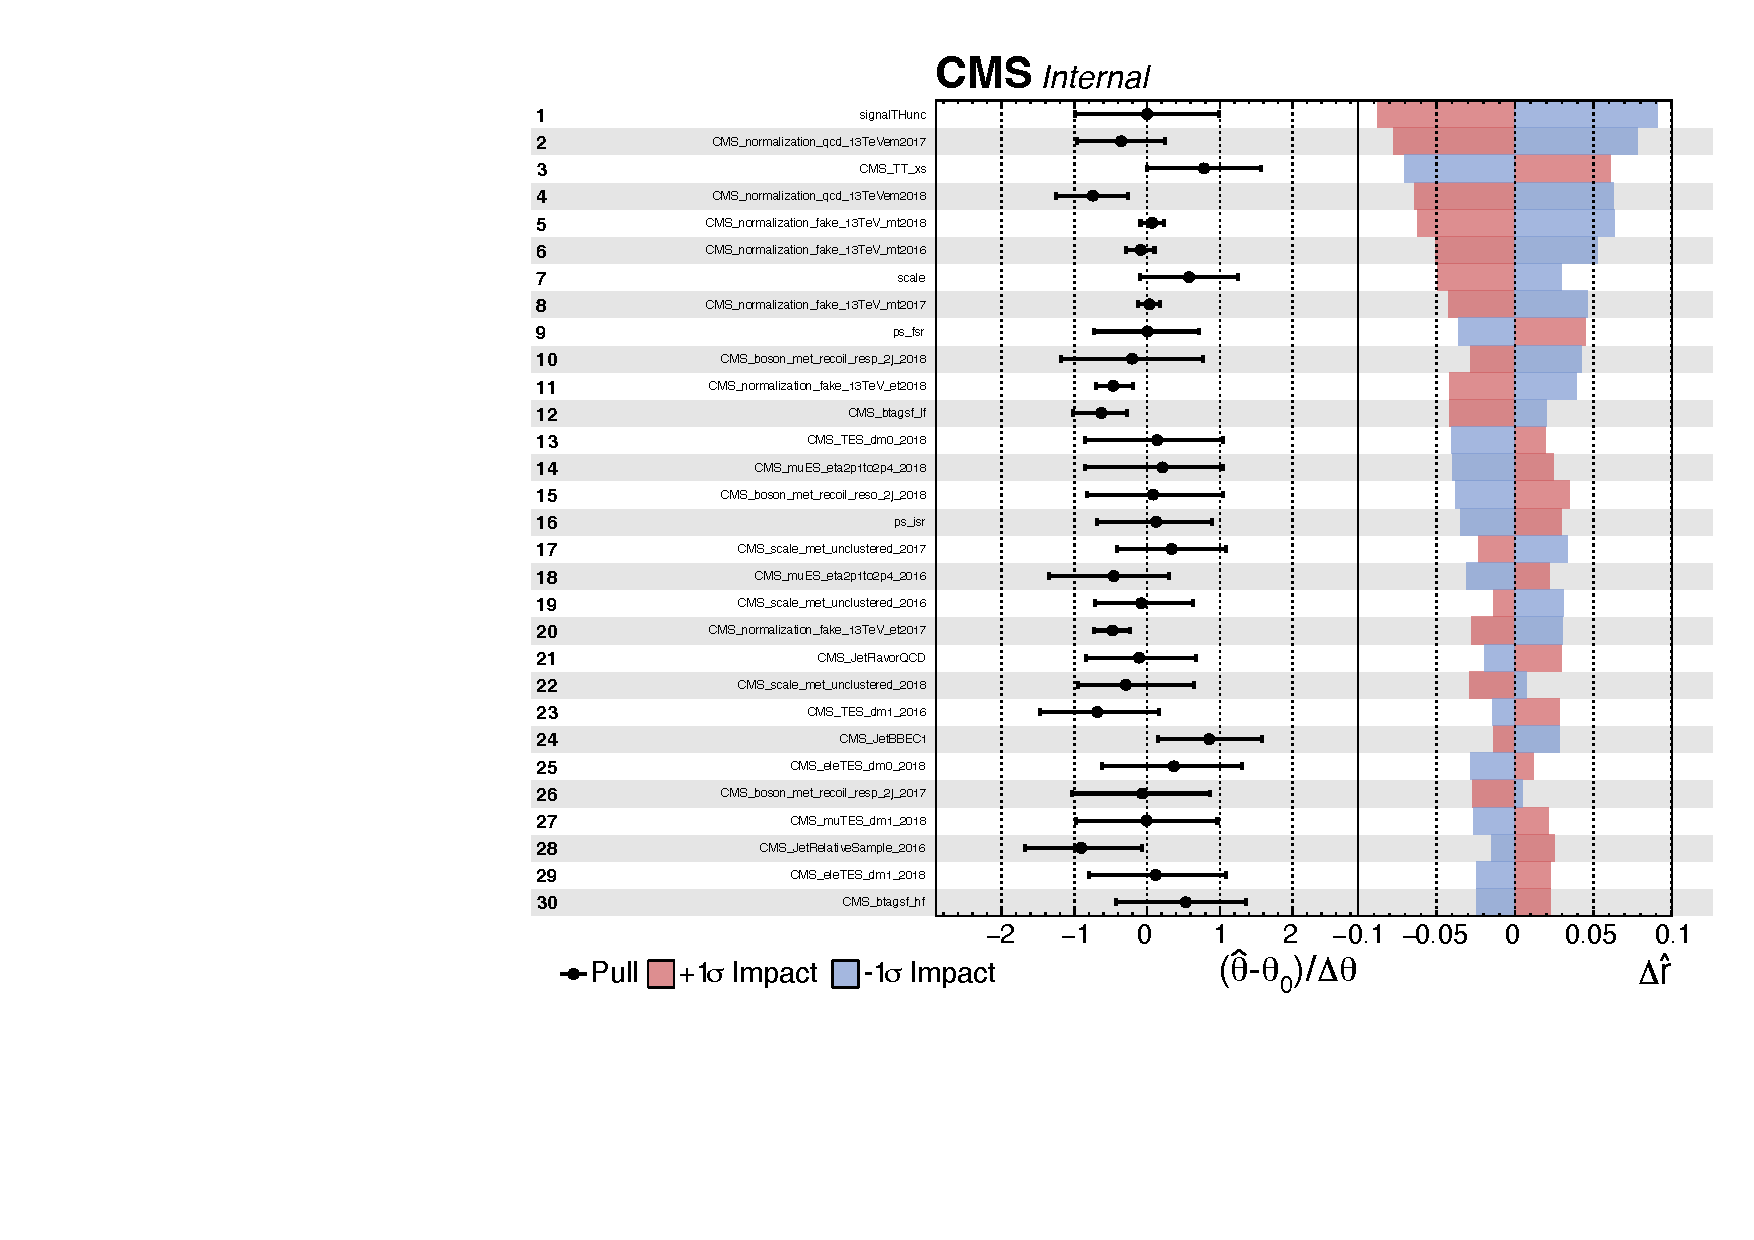
\includegraphics[width=0.8\textwidth]{figures/ch-8-systematic-uncertainties/impacts-all-1.pdf}\\
        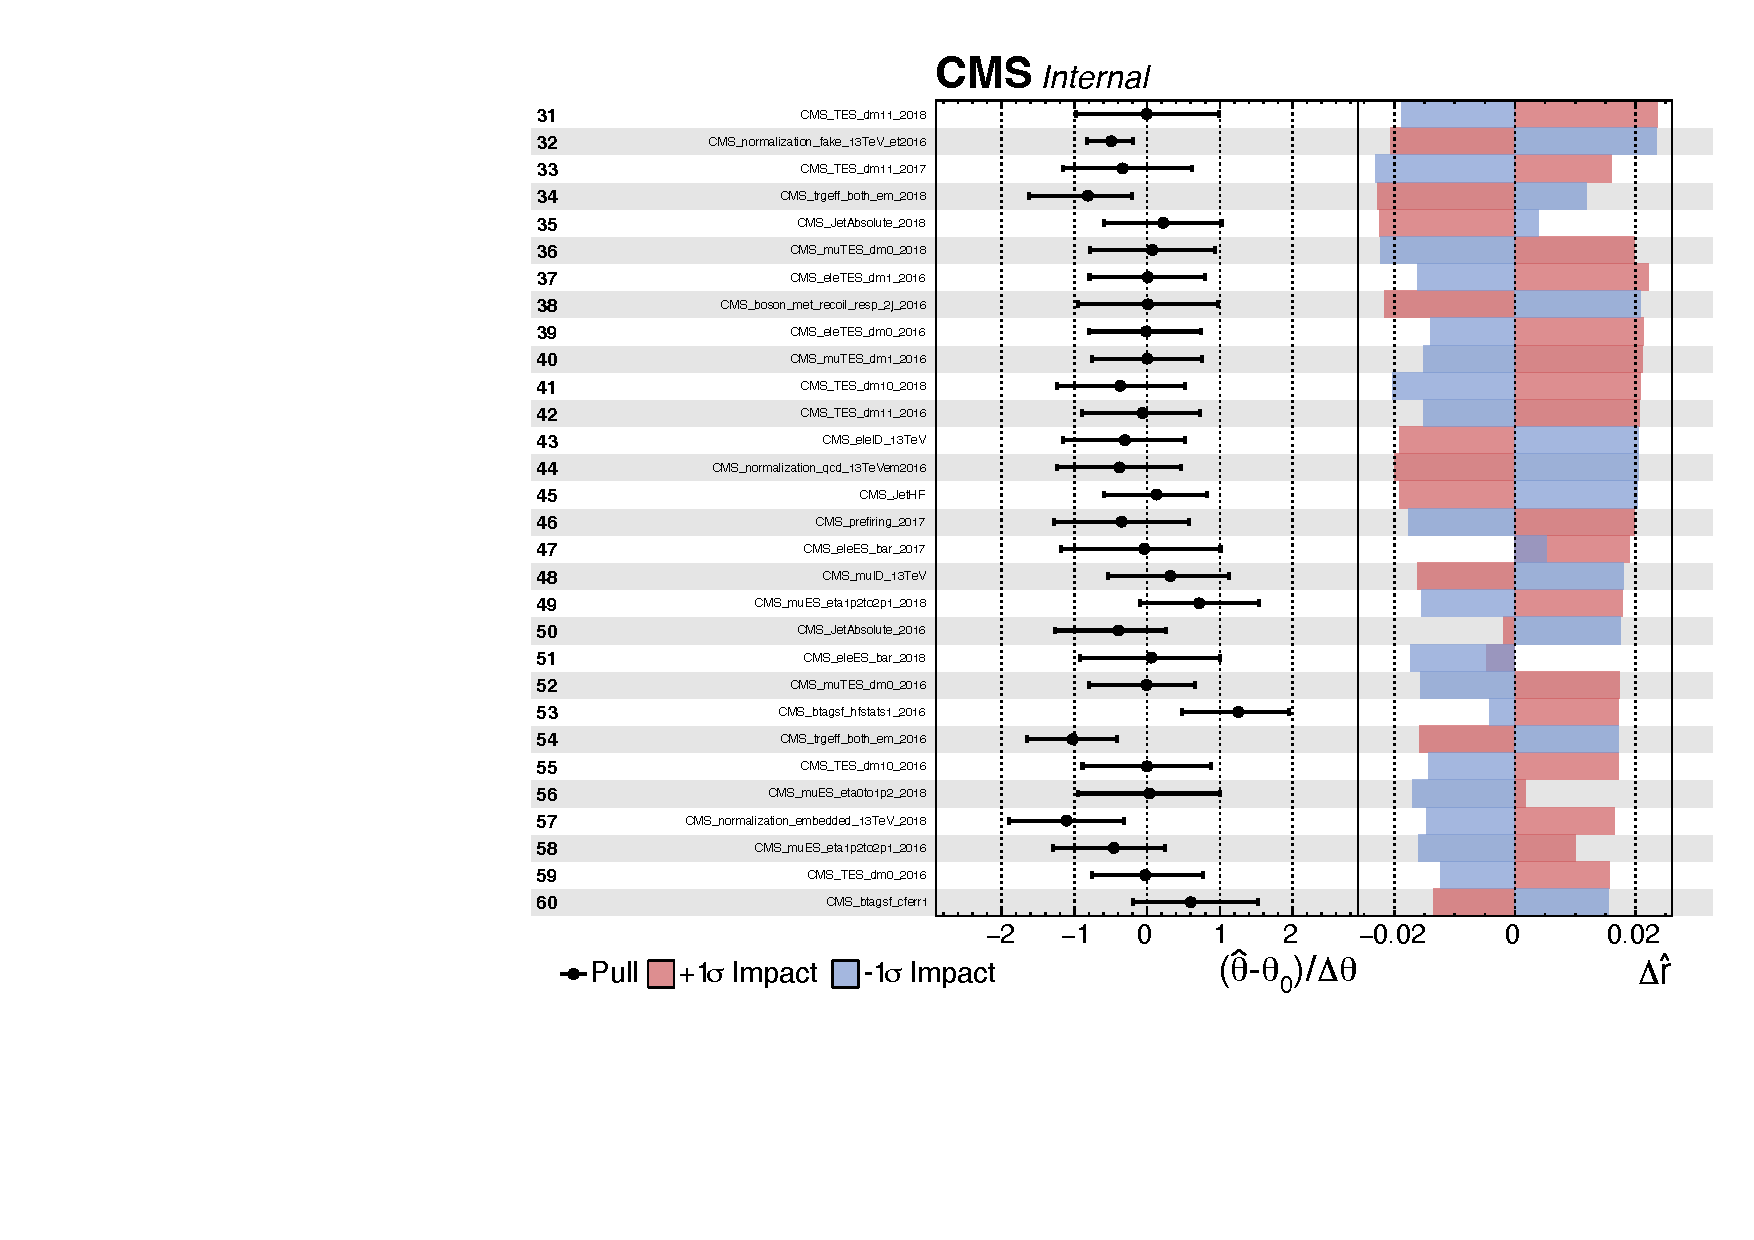
\includegraphics[width=0.8\textwidth]{figures/ch-8-systematic-uncertainties/impacts-all-2.pdf}
    \end{center}
    \caption[Top sixty pulls and impacts for the combination of all channels and years.]{Top sixty pulls and impacts for the combination of all channels and years~\cite{CMS-AN-20-213}.}
    \label{fig:impacts_pages_1_2}
\end{figure}


\chapter{Event categorization and signal extraction}
\label{chapter:ch-9:event-categorization-signal-extraction}
\section{B-tag jet multiplicity}
The increased statistics of the full Run-2 dataset enables the separation of events into events with exactly 1 b-tag jet and events with greater than 1 b-tag jet. Further event categorization is performed with deep neural networks (DNNs) described below. The DNNs  are used only for separating events into signal and control regions in the 1 b-tag and 2 b-tag jets scenarios. The final results are extracted from the statistical fitting to the mass of the $\tau\tau$, $m_{\tau\tau}$.

\section{DNN-based event categorization}
A brief overview of the DNN-based event categorization is given below with a focus on the physics aspects, with full details of the machine learning training in \cite{CMS-HIG-22-007} and associated documentation.

\subsubsection{Training samples}
Neural networks for event categorization are trained for each of the $\mu\tau_{h}$, $e\tau_{h}$, and $e\mu$ channels, for 1 and 2 b-tag jets, giving $3 \times 2 = 6$ networks in total. In the training, the signal is taken to be all of the possible pseudoscalar mass $m_{a}$ hypotheses together. The backgrounds for each DNN are taken to be a representative combination of the three major backgrounds: $Z \rightarrow \tau\tau$, $t\bar{t}$+jets, and fake backgrounds. The proportions of each background for each channel and b-tag jet multiplicity are taken from the yields in the $m_{\tau\tau}$ distribution. For instance, in the $\mu\tau_{h}$ 1 b-tag jet category, the composition of the background for training is 17.4\% from $Z \rightarrow \tau\tau$, 42.4\% from $t\bar{t}$+jets, and 40.2\% fakes.

\subsubsection{Input variables}
The input variables capture the key differences between the signal and the background:
\begin{itemize}
    \item Transverse momentum $p_{T}$ of the electron and muon in the $e\tau_{h}$ and $\mu\tau_{h}$ channels, where the signal tends to have a softer $p_{T}$ spectrum (lower energy) than the background.
    \item $p_{T}$ of the b-tag jet(s). The signal sample b-tag jet(s) tend to have softer $p_{T}$.
    \item Invariant masses of the various objects ($\tau\tau$ legs and the b-tag jet(s)), which tend to be smaller for the signal samples.
    \item The angular separation $\Delta R$ between pairs of the objects, where signal samples peak at smaller $\Delta R$ values.
    
    \item The transverse mass between the missing transverse energy $p_{T}^{\text{miss}}$ and each of the four objects \cite{CMS-HIG-17-024}, defined as
        \begin{equation}
            m_{T}(\ell, p_{T}^{\text{miss}}) \equiv \sqrt{2 p_{T}^{\ell} \cdot p_{T}^{\text{miss}} [1 - \cos(\Delta \phi)]}
        \end{equation}
    where $p_{T}^\ell$ is the transverse momentum of the object $\ell$, and $\Delta \phi$ is the difference in azimuthal angle between the object and the $p_{T}^{\text{miss}}$. Events from $t\bar{t}$+jets and jets faking $\tau_{h}$ backgrounds have larger $p_{T}^{\text{miss}}$ resulting in larger transverse mass values compared to the signal, which tends to have smaller $p_{T}^{\text{miss}}$ that is also more aligned with the lepton legs.

    \item The variable $D_{\zeta}$ \cite{CMS-HIG-17-024}, defined as
        \begin{equation}
            D_{\zeta} \equiv p_{\zeta} - 0.85 p_{\zeta}^{\text{vis}}
        \end{equation}
        where the $\zeta$ axis is the bisector of the transverse directions of the visible $\tau$ decay products. $p_{\zeta}$ is the compomnent of the $p_{T}^{\text{miss}}$ along the $\zeta$ axis, and $p_{\zeta}^{\text{vis}}$ is the sum of the components of the lepton $p_{T}$ along the same axis. This variable captures the fact that in signal the $p_{T}^\text{miss}$ is small and approximately aligned with the $\tau\tau$. In contrast, the $Z \rightarrow \tau\tau$ background tends towards large $D_{\zeta}$ values because the $p_{T}^{\text{miss}}$ is collinear to the $\tau\tau$, and the $t\bar{t}$+jets events tend to have small $D_{\zeta}$ due to a large $p_{T}^{\text{miss}}$ not aligned with the $\tau\tau$.

    \item For events with 2 b-tag jets, one additional variable is defined to capture the difference in the invariant mass of the $bb$ and the $\tau\tau$:
        \begin{equation}
            \Delta m_{a_1} \equiv (m_{bb} - m_{\tau\tau})/{m_{\tau\tau}}
        \end{equation}
    This variable peaks at zero for the $h\rightarrow aa \rightarrow 2b2\tau$ signal.
\end{itemize}

\subsubsection{Categorization using the DNN score}

After training, events in data, MC, and embedded are evaluated with the six DNNs and assigned a raw score between 0 and 1 (background-like or signal-like). In order to flatten the distribution of the score and define score thresholds for categorizing events, the raw output scores are transformed with the function $\tilde{p}(n) = \arctanh(p \times \tanh(n))/n$ where $n$ is a positive integer. The thresholds of the DNN score used for signal/control region definition are determined using scans that optimize the signal sensitivity and are shown in Tables \ref{table:1bNN-final-categories} and \ref{table:2bNN-final-categories}.

\begin{table}[h!]
    \begin{center}
       \begin{tabular}{|c|c|c|c|c|}
       \hline
        & \multicolumn{3}{c}{1bNN $\tilde{p}(n=1.5)$} & \\
       \hline
        & SR1 & SR2 & SR3 & CR \\
       \hline
       $\mu\tau_{h}$ 2018 & $>$ 0.98 & $\in[0.95,0.98]$ & $\in[0.90, 0.95]$ & $<0.90$ \\
       $\mu\tau_{h}$ 2017 & $>$ 0.97 & $\in[0.94,0.97]$ & $\in[0.90, 0.94]$ & $<0.90$ \\
       $\mu\tau_{h}$ 2016 & $>$ 0.97 & $\in[0.94,0.97]$ & $\in[0.89, 0.94]$ & $<0.89$ \\
       \hline
       \hline
        & \multicolumn{3}{c}{1bNN $\tilde{p}(n=1.5)$} & \\
       \hline
        & SR1 & SR2 & SR3 & CR \\
       \hline
       $e\tau_{h}$ 2018 & $>$ 0.97 & $\in[0.945,0.97]$ & $\in[0.90, 0.945]$ & $<0.90$ \\
       $e\tau_{h}$ 2017 & $>$ 0.985 & $\in[0.965,0.985]$ & $\in[0.93, 0.965]$ & $<0.93$ \\
       $e\tau_{h}$ 2016 & $>$ 0.985 & $\in[0.965,0.985]$ & $\in[0.93, 0.965]$ & $<0.93$ \\
       \hline
       \hline
        & \multicolumn{3}{c}{1bNN $\tilde{p}(n=2.5)$} & \\
       \hline
        & SR1 & SR2 & SR3 & CR \\
       \hline
       $e\mu$ 2018 & $>$ 0.99 & $\in[0.95,0.99]$ & $\in[0.85, 0.95]$ & $<0.85$ \\
       $e\mu$ 2017 & $>$ 0.985 & $\in[0.95,0.985]$ & $\in[0.85, 0.95]$ & $<0.85$ \\
       $e\mu$ 2016 & $>$ 0.99 & $\in[0.95,0.99]$ & $\in[0.85, 0.95]$ & $<0.85$ \\
       \hline
      \end{tabular}
    \end{center}
    \caption{Event categorization based on DNN scores for events with exactly 1 b-tag jet (1bNN), for the three $\tau\tau$ channels and three eras.}
    \label{table:1bNN-final-categories}
\end{table}


\begin{table}[h!]
    \begin{center}
       \begin{tabular}{|c|c|c|c|}
       \hline
        & \multicolumn{2}{c}{2bNN $\tilde{p}(n=1.5)$} & \\
       \hline
        & SR1 & SR2 & CR \\
       \hline
       $\mu\tau_{h}$ 2018 & $>0.99$ & $\in[0.96,0.99]$ & $<0.96$ \\
       $\mu\tau_{h}$ 2017 & $>0.98$ & $\in[0.94,0.98]$ & $<0.94$ \\
       $\mu\tau_{h}$ 2016 & $>0.97$ & $\in[0.93,0.97]$ & $<0.93$ \\
       \hline
       \hline
        & \multicolumn{2}{c}{2bNN $\tilde{p}(n=1.5)$} & \\
       \hline
        & SR1 & SR2 & CR \\
       \hline
       $e\tau_{h}$ 2018 & $>0.96$ & NA & $<0.96$ \\
       $e\tau_{h}$ 2017 & $>0.985$ & NA & $<0.985$ \\
       $e\tau_{h}$ 2016 & $>0.96$ & NA & $<0.96$ \\
       \hline
       \hline
        & \multicolumn{2}{c}{2bNN $\tilde{p}(n=2.5)$} & \\
       \hline
        & SR1 & SR2 & CR \\
       \hline
       $e\mu$ 2018 & $>0.98$ & $\in[0.94,0.98]$ & $<0.94$ \\
       $e\mu$ 2017 & $>0.97$ & $\in[0.93,0.97]$ & $<0.93$ \\
       $e\mu$ 2016 & $>0.98$ & $\in[0.94,0.98]$ & $<0.94$ \\
       \hline
      \end{tabular}
    \end{center}
    \caption{Event categorization based on DNN scores for events with 2 b-tag jets (2bNN), for the three $\tau\tau$ channels and three eras.}
    \label{table:2bNN-final-categories}
\end{table}


\section{Methodology for signal extraction}
In this section we outline the statistics terminology and concepts underlying the modified frequentist method $CL_{S}$ used to perform signal extraction.

\subsection{Model building and parameter estimation}
In the frequentist interpretation of probability, an experiment measuring an observable can be repeated, resulting in different values of the observable, e.g. the invariant mass of a candidate Higgs boson in a search for the Higgs \cite{2011-Statistics-Cranmer}. The ensemble of values of the observable $x$ gives rise to the probability density function (PDF) $f(x)$, which has the important property that it is normalized to unity:
\begin{equation*}
    \int f(x) \, dx = 1 \,.
\end{equation*}
A parametric family of PDFs
\begin{equation*}
    f(x|\alpha) \, ,
\end{equation*}
read ``$f$ of $x$ given $\alpha$", is referred to as a probability model or model. The parameters $\alpha$ typically represent parameters of the theory or an unknown property of the detector's response. The parameters are not frequentist in nature, unlike $x$. Out of all the parameters, typically only a few are of interest, and are called the parameters of interest (POI), labeled $\mu$ here. The remaining are referred to as nuisance parameters (NP) \cite{2011-Statistics-Cranmer} and are labeled $\boldsymbol{\theta}$.

$f(x)$ is the probability density for the observable in one event and we wish to describe the probability density for a dataset with many events, $\mathcal{D} = \{x_1, ..., x_n\}$, called the total probability model $\boldsymbol{f}$. For instance, if we also have a prediction for the total number of events expected, called $\nu$, we also account for the overall Poisson probability for observing $n$ events given $\nu$ expected:
\begin{equation}
    \boldsymbol{f}(\mathcal{D}|\nu, \alpha) = \text{Poisson}(n|\nu) \prod_{e=1}^{n} f(x_e | \alpha)
\end{equation}

The likelihood function $L(\alpha)$ is numerically equivalent to $f(x|\alpha)$ for fixed $x$, or $\boldsymbol{f}(\mathcal{D}|\alpha)$ with $\mathcal{D}$ fixed \cite{2011-Statistics-Cranmer}. The likelihood function is not a probability density for $\alpha$ and is not normalized to unity:
\begin{equation*}
    \int L(\alpha) \, d(\alpha) \neq 1 \, .
\end{equation*}
i.e. the likelihood function is the value of $f$ as a function of $\alpha$ given a fixed value of $x$.

To estimate the parameter $\alpha$ we use an estimator, which is a function of the data. Take for example the measurement of data distributed according to a Gaussian probability density $f(x| \mu,\sigma) = \text{Gauss}(x|\mu,\sigma)$. One possible estimator of the mean $\mu$, is the mean of the measured data points $\bar{x} = \sum_{i = 1}^{n} x_i / n$ \cite{2011-Statistics-Cranmer}. 

A commonly used estimator in physics is the maximum likelihood estimator (MLE), defined as the value $\alpha$ which maximizes the likelihood function $L(\alpha)$. This value, labeled $\hat{\alpha}$, also maximizes $\ln L(\alpha)$ and minimizes $-\ln L(\alpha)$. By convention the $-\ln L(\alpha)$ is minimized, in a process called ``fitting", and the maximum likelihood estimate is called the ``best fit value". 


% Profile likelihood ratios

% How to get a Confidence Level 

% Asimov dataset

\subsection{Hypothesis testing}
In this section we next introduce concepts related to hypothesis testing such as the test statistic constructed from the ratio of likelihood functions.

The objective of a likelihood analysis is to distinguish different models representing the various hypotheses, and determine the one that best explains the experimental outcome. In a search for new physics, a signal is additive on top of the background. The background-only hypothesis is the null hypothesis, and the signal-plus-background hypothesis is the alternative. 

As a simple example, take the $p$-value test, for an experiment where we count events in the signal region, $n_{SR}$, and expect $\nu_B$ background events and $\nu_S$ events from the signal \cite{2011-Statistics-Cranmer}. Then 
\begin{enumerate}
    \item The null hypothesis ($H_0$), i.e. the background-only hypothesis in this experiment, with the probability modeled by Poisson($n_{SR}|\nu_B$).
    \item The alternate hypothesis ($H_1$), i.e. signal-plus-background hypothesis, with the probability modeled by Poisson($n_{SR}|(\nu_B + \nu_S)$).
\end{enumerate}
The compatibility of the observed data $\nu^0_{SR}$ and the null hypothesis, is quantified as the probability that the background-only hypothesis would produce at least as many events as was observed. This probability is the $p$-value: 
\begin{equation}
    p = \sum_{n = n^0_{SR}}^{\infty} \text{Poisson}(n | \nu_B) \, .
\end{equation}
If the $p$-value is very small, we might reject the null hypothesis. The $p$-value is not the probability of the null hypothesis given the data; rather, it expresses the probability that data with a certain property was obtained, assuming the null hypothesis \cite{2011-Statistics-Cranmer}.

The $p$-value is an example of a test statistic $T$, which maps the data to a single real number. The Neyman-Pearson lemma states that out of the infinite possibilities of choices of test statistic, the uniformly most powerful test statistic is the likelihood ratio $T_{NP}$ \cite{2011-Statistics-Cranmer}:

\begin{equation}
    T_{NP}(\mathcal{D}) = \frac{L(\mathcal{D} | {H_1})}{L(\mathcal{D}|{H_0})}
\end{equation}
To reiterate, the test statistic $T$ is a real-valued function of the data, implying that a particular probability model $\boldsymbol{f}(\mathcal{D}|\boldsymbol{\alpha})$ implies a distribution of the test statistic, $f(T|\boldsymbol{\alpha})$, which depends on the value of $\alpha$. With this distribution in hand, the $p$-value can be evaluated in the following equivalent formulations:
\begin{align}
    p(\boldsymbol{\alpha}) &= \int_{T_0}^{\infty} f(T|\boldsymbol{\alpha}) \, dT  \\
              &= \int \boldsymbol{f}(\mathcal{D} | \boldsymbol{\alpha}) \, \theta(T(\mathcal{D}) - T_0) \, d\mathcal{D} \\
              &= P(T \geq T_0 | \boldsymbol{\alpha})
\end{align}
where $T_0$ is the value of $T$ based on the observed data, and $\theta()$ is the Heaviside function. The size of the test is conventionally chosen to be 10\%, 5\%, or 1\%. As the $p$-value depends on $\boldsymbol{\alpha}$ (both the POI and NP), the null hypothesis should not be rejected if the $p$-value is larger than the size of the test for any value of the nuisance parameters.

\subsection{Confidence intervals}
In an example of the measurement of the Standard Model Higgs boson, $\boldsymbol{\alpha}_{\text{POI}} = (\sigma/ \sigma_{SM}, M_H)$, with $\sigma/\sigma_{SM}$ is the ratio of the production cross-section for Higgs with respect to its value in the SM, and $M_H$ is the unknown mass of the Higgs, values of these parameters outside specific bounds are said to be ``excluded at the 95\% confidence level''. These allowed regions are called confidence levels or confidence regions, and the parameter values outside of them are considered excluded \cite{2011-Statistics-Cranmer}. A 95\% confidence interval does not mean that there is a 95\% chance that the true value of the parameter is inside the interval. Rather, a 95\% confidence interval covers the true value 95\% of the time (even though we do not know the true value). 

To construct a confidence interval for a parameter $\alpha$, the Neyman Construction is used to invert a series of hypothesis tests; i.e. for each possible value of $\alpha$, the null hypothesis is treated as $\alpha$, and we perform a hypothesis test based on a test statistic. To construct a 95\% confidence interval, we construct a series of hypothesis tests with size of 5\%. The confidence interval $I(\mathcal{D})$ is constructed by taking the set of parameter values $\boldsymbol{\alpha}$ where the null hypothesis is accepted:
\begin{equation}
    I(\mathcal{D}) = \{ \boldsymbol{\alpha} | P(T(\mathcal{D}) > k_\alpha | \boldsymbol{\alpha}) < \alpha \} \, ,
\end{equation} 
where $T(\mathcal{D})$ is the test statistic, and the last $\alpha$ (not bolded) and the subscript $k_\alpha$ refer to the size of the test. A schematic of the Neyman construction is shown in Fig. \ref{fig:neyman-construction}. In a more generalized case, the $x$-axis is the test statistic $T$.

\begin{figure}[ht]
    \centering
    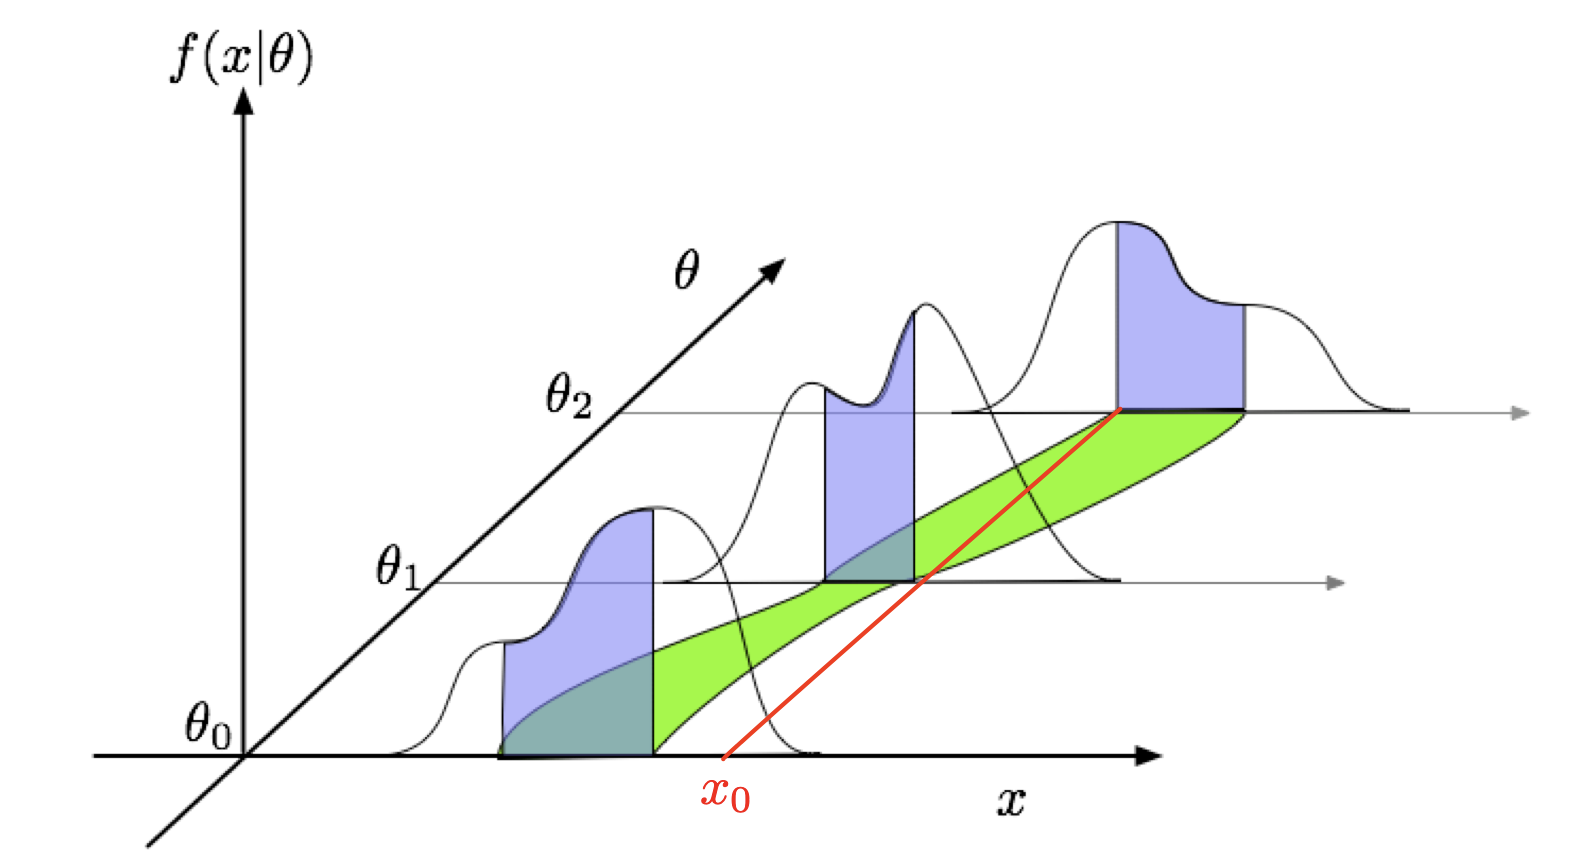
\includegraphics[width=12cm]{figures/ch-9-event-categorization-and-signal-extraction/schematic_neyman_construction.png}
    \caption[Schematic of the Neyman construction for confidence intervals.]{Schematic of the Neyman construction for confidence intervals \cite{2011-Statistics-Cranmer}. For each value of $\theta$, we find a region in $x$ where $\int f(x|\theta) dx$ satisfies the size of the test (\textit{blue}). These regions form a confidence belt (\textit{green}). The intersection of the observation $x_0$ (\textit{red}) with the confidence belt defines the confidence interval $[\theta_1, \theta_2]$ \cite{2011-Statistics-Cranmer}.} 
    \label{fig:neyman-construction}
\end{figure}

\subsection{Profile likelihood ratio}

In this section we describe a frequentist statistical procedure based on the profile likelihood ratio test statistic, which is implemented using asymptotic distributions.

With a multi-parameter likelihood function $L(\boldsymbol{\alpha})$, the the maximum likelihood of one specific parameter $\alpha_p$ with other parameters $\boldsymbol{\alpha}_o$ fixed, is called the conditional maximum likelihood estimate and is denoted $\doublehat{\alpha}_p(\boldsymbol{\alpha_0})$.
The process of choosing specific values of the nuisance parameters for a given value of $\mu$, $\mathcal{D}_{\text{simulated}}$, and value of global observables $\mathcal{G}$ is called profiling. From the full list of parameters $\boldsymbol{\alpha}$, we denote the parameter of interest $\mu$, and the nuisance parameters $\boldsymbol{\theta}$.

We construct the profile likelihood ratio,
\begin{equation}
    \lambda(\mu) = \frac{L(\mu, \doublehat{\boldsymbol{\theta}}(\mu))}{L({\mu, \hat{\boldsymbol{\theta}}})}
\end{equation}
which depends explicitly on the parameter of interest $\mu$, implicitly on the data $\mathcal{D}_{\text{sim}}$ and global observables $\mathcal{G}$, and is independent of the nuisance parameters $\boldsymbol{\theta}$, which have been eliminated in profiling \cite{2011-Statistics-Cranmer}.

The main conceptual reason for constructing the test statistic from the profile likelihood ratio is that asymptotically (i.e. for measurements with many events) the distribution of the profile likelihood ratio $\lambda(\mu = \mu_{\text{true}})$ is independent of the values of the nuisance parameters \cite{2011-Statistics-Cranmer}. 

The following $p$-value is used to quantify the consistency with the hypothesis of a signal strength of $\mu$:
\begin{equation}
    p_\mu = \int_{\tilde{q}_{\mu, \text{obs}}}^{\infty} f(\tilde{q}_\mu | \mu, \doublehat{\boldsymbol{\theta}}(\mu, \text{obs})) \, d\tilde{q}_\mu
\end{equation}


\subsection{Modified frequentist method: $CL_{S}$}
In the modified frequentist method called $CL_{S}$, to test a hypothesis with signal, we define $p'_{\mu}$ as a ratio of $p$-values \cite{2011-Statistics-Cranmer}:
\begin{equation}
    p'_{\mu} = \frac{p_\mu}{1 - p_b}
\end{equation}
where $p_b$ is the $p$-value derived under the background-only hypothesis:
\begin{equation}
    p_b = 1 - p_0 \equiv 1 - \int_{\tilde{q}_{\mu, \text{obs}}}^{\infty} f(\tilde{q}_\mu | 0, \doublehat{\boldsymbol{\theta}}(\mu = 0, \text{obs})) \, d\tilde{q}_{\mu} \, .
\end{equation}
The $CL_{S}$ upper limit on $\mu$, denoted $\mu_{up}$, is obtained by solving for $p'_{\mu_{\text{up}}} = 5\%$. If testing the compatibility of the data with the background-only hypothesis, we consider the $p_b$ value defined above and conventionally convert it into the quantile or ``sigma" of a unit Gaussian. $z$ standard deviations (e.g. $z = 5$ in ``5$\sigma$") means that the probability of falling above these standard deviations, equals $p_b$ (e.g. $3\sigma$ corresponds to $p_b = 2.7 \times 10^{-3}$ or 95.43\%, and $5\sigma$ corresponds to $p_b = 5.7 \times 10^{-7}$ or 99.999943\%).


\chapter{Results}
In this chapter, Section \ref{section:bbtautau_results} presents the results from the $h \rightarrow aa \rightarrow bb\tau\tau$ analysis performed on 137 fb$^{-1}$ of data from the full CMS Run-2 dataset in the years 2016 to 2018, with interpretations provided for different 2HDM+S scenarios. This analysis was combined with a different search in the $h\rightarrow aa \rightarrow bb\mu\mu$ final state, which was also performed on the full Run-2 dataset. The combination procedure and results from the combined analyses ($h \rightarrow aa \rightarrow bb\ell\ell$, with $\ell = \mu, \tau$) are detailed in Sectopm \ref{section:combination-procedure-with-bbmumu}. The combined analysis places some of the most stringent limits to date at CMS for 2HDM+S scenarios in the light scalar mass range $m_a = 12$\GeV to 60 \GeVns.

\section{Results from \texorpdfstring{$bb\tau\tau$}{bbtautau}}
\label{section:bbtautau_results}
In each of the three $\tau\tau$ channels studied ($\mu\tau_{h}$, $e\tau_{h}$, and $e\mu$), events are divided based on whether they contain exactly 1 or 2 b-tag jets, and further divided into signal and control regions (SRs and CRs) using the DNN categorization score as described in Section \ref{section:DNN-event-categorization}. The control regions demonstrate good agreement between observed events in data, and the sum of the contributions from expected backgrounds that are modeled in simulated and embedded samples. The signal regions are defined to be sensitive to the $h \rightarrow aa \rightarrow bb\tau\tau$ signal. The postfit final observed and expected distributions of the di-tau invariant mass $m_{\tau\tau}$ reconstructed with SVFit (described in Section \ref{section:svfit}) are shown in Fig. \ref{fig:results_mtt_postfit_mtall} for the $\mu\tau_{h}$ channel, Fig. \ref{fig:results_mtt_postfit_etall} for the $e\tau_{h}$ channel, and Fig. \ref{fig:results_mtt_postfit_emall} for the $e\mu$ channel. In all figures, the hypothesized yield for the $h\rightarrow aa \rightarrow bb\tau\tau$ signal is shown for the pseudoscalar mass $m_a = 35$ GeV and assuming a branching fraction $B(h \rightarrow aa \rightarrow bb\tau\tau) = 10\%$.
\begin{figure}[ht]
    \begin{center}
        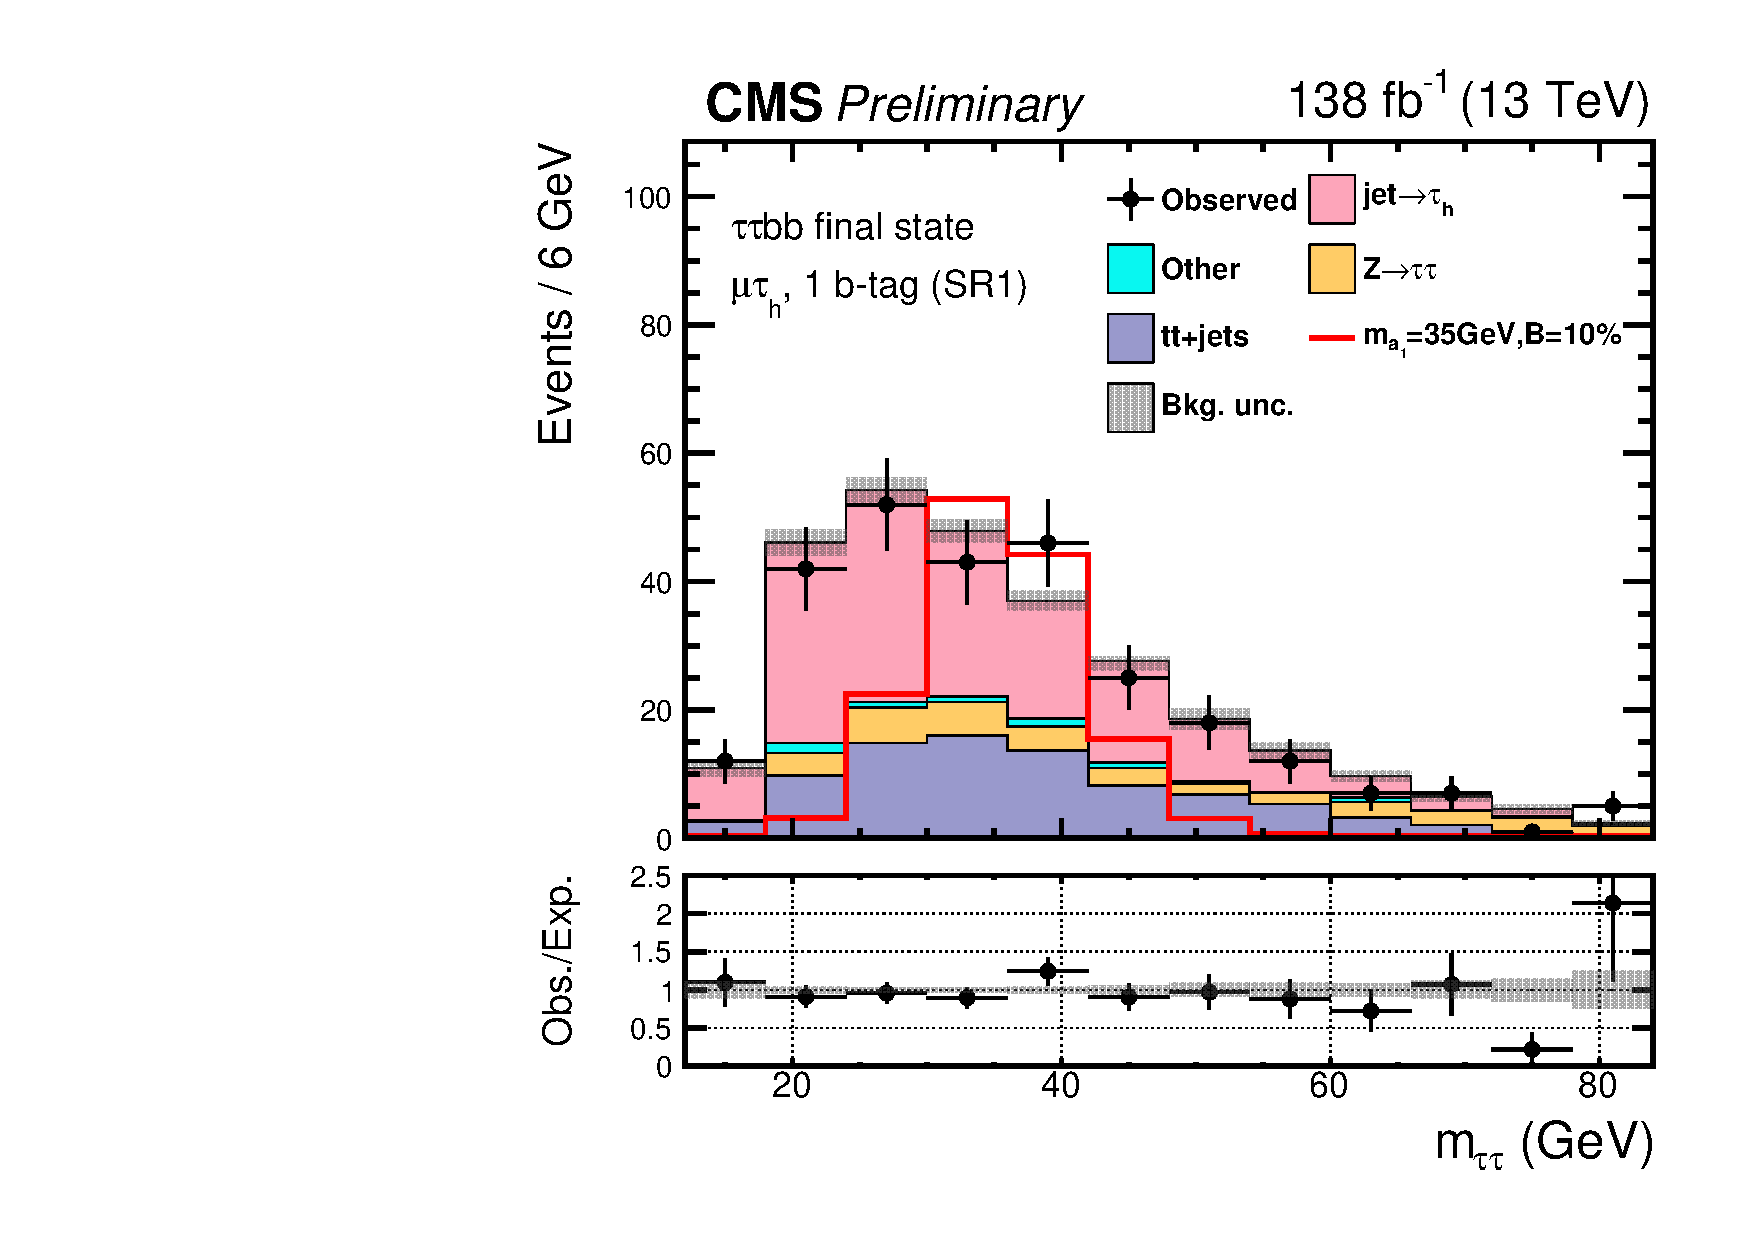
\includegraphics[width=0.32\textwidth]{figures/ch-10-results/mt_all_1_post_prelim-yes.pdf}
        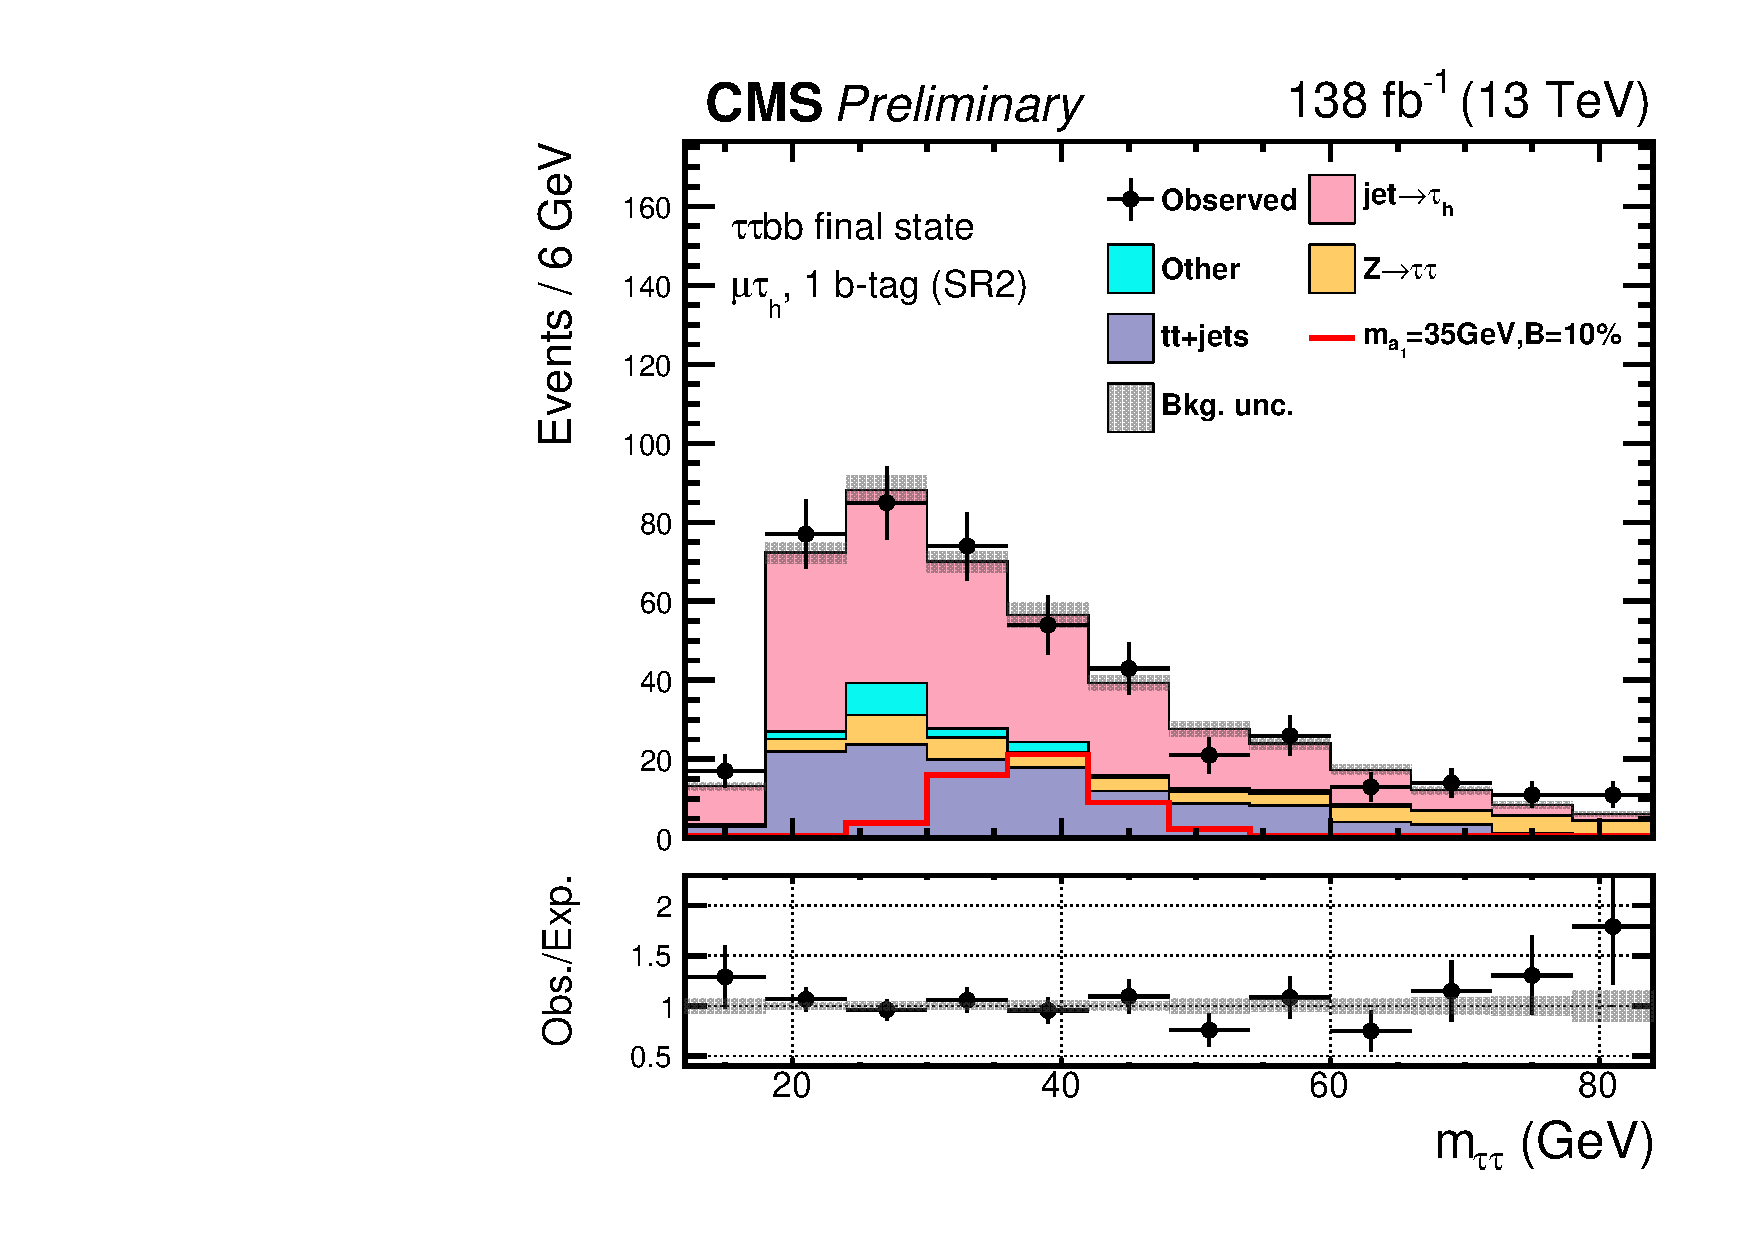
\includegraphics[width=0.32\textwidth]{figures/ch-10-results/mt_all_2_post_prelim-yes.pdf}
        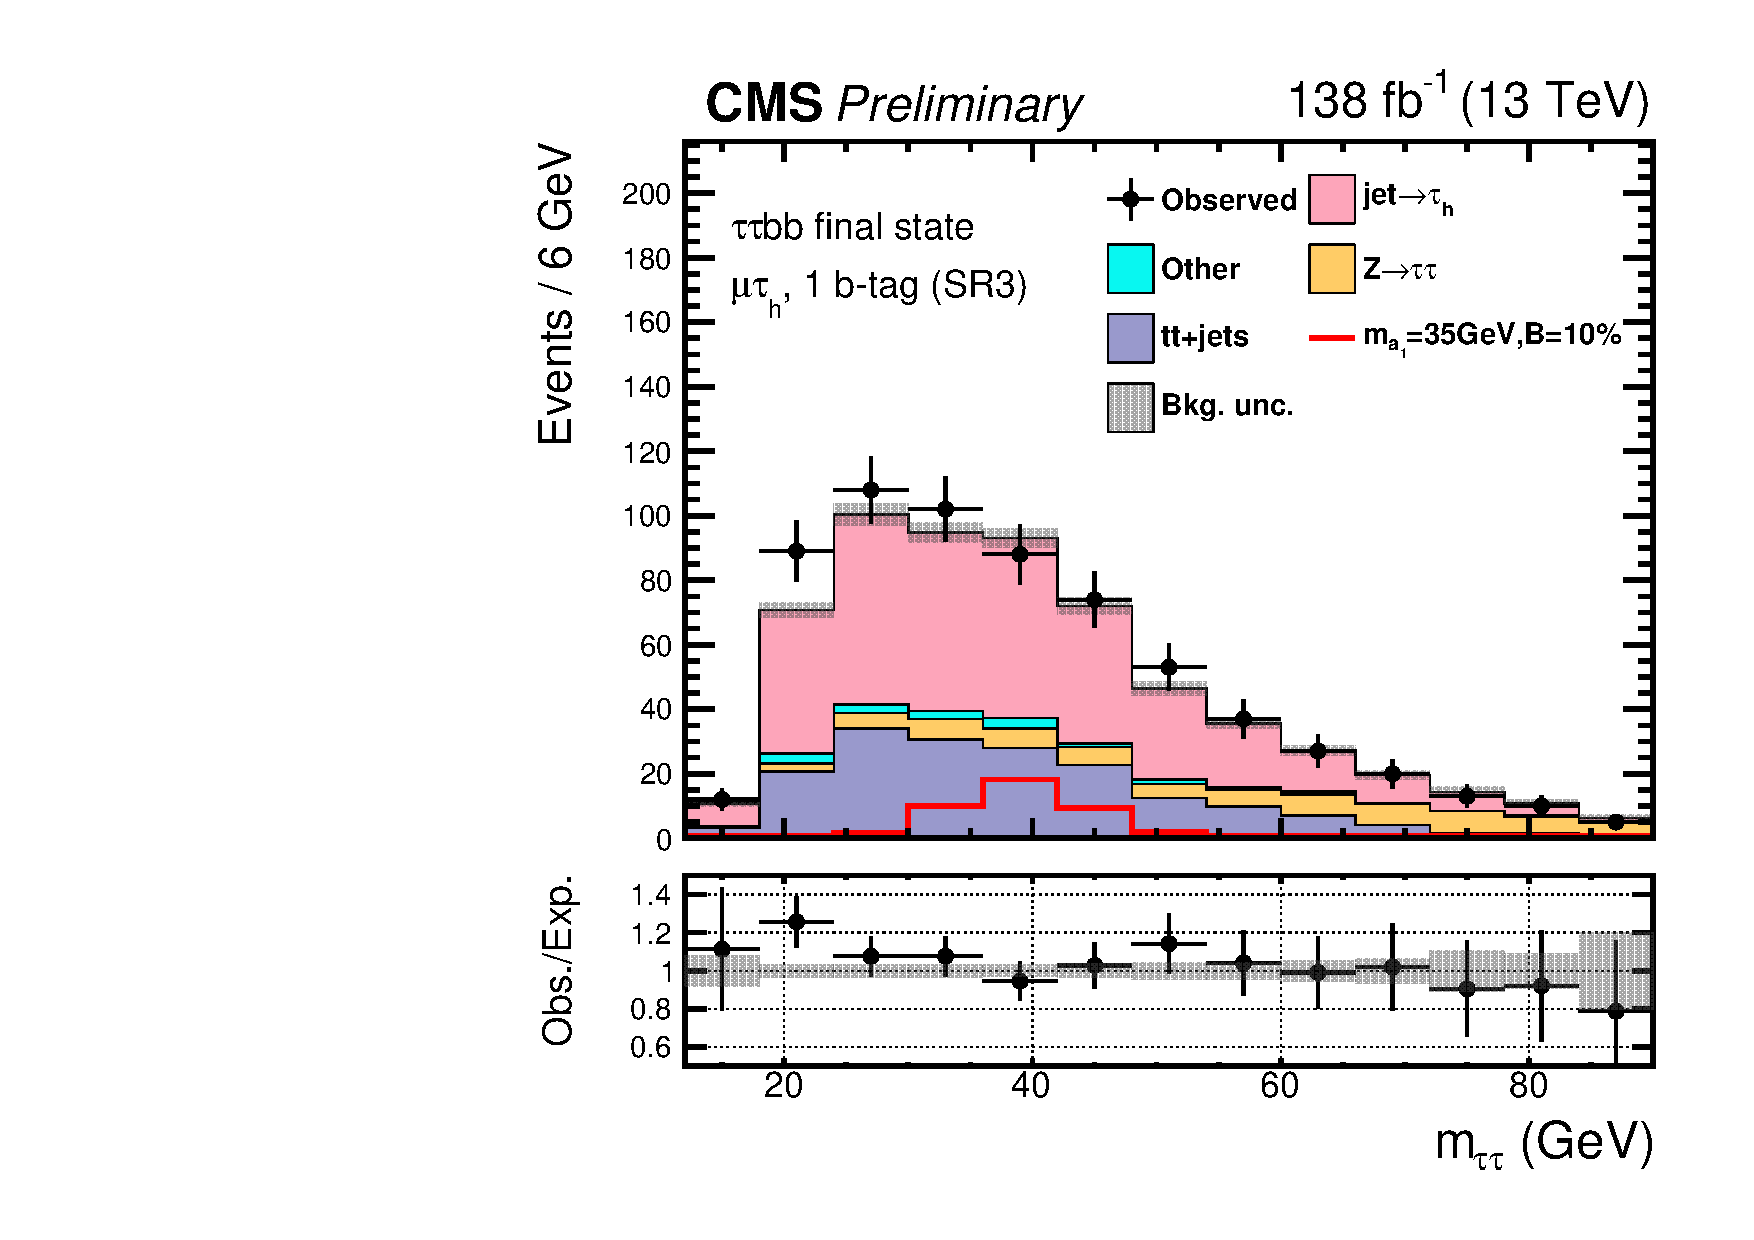
\includegraphics[width=0.32\textwidth]{figures/ch-10-results/mt_all_3_post_prelim-yes.pdf}\\
        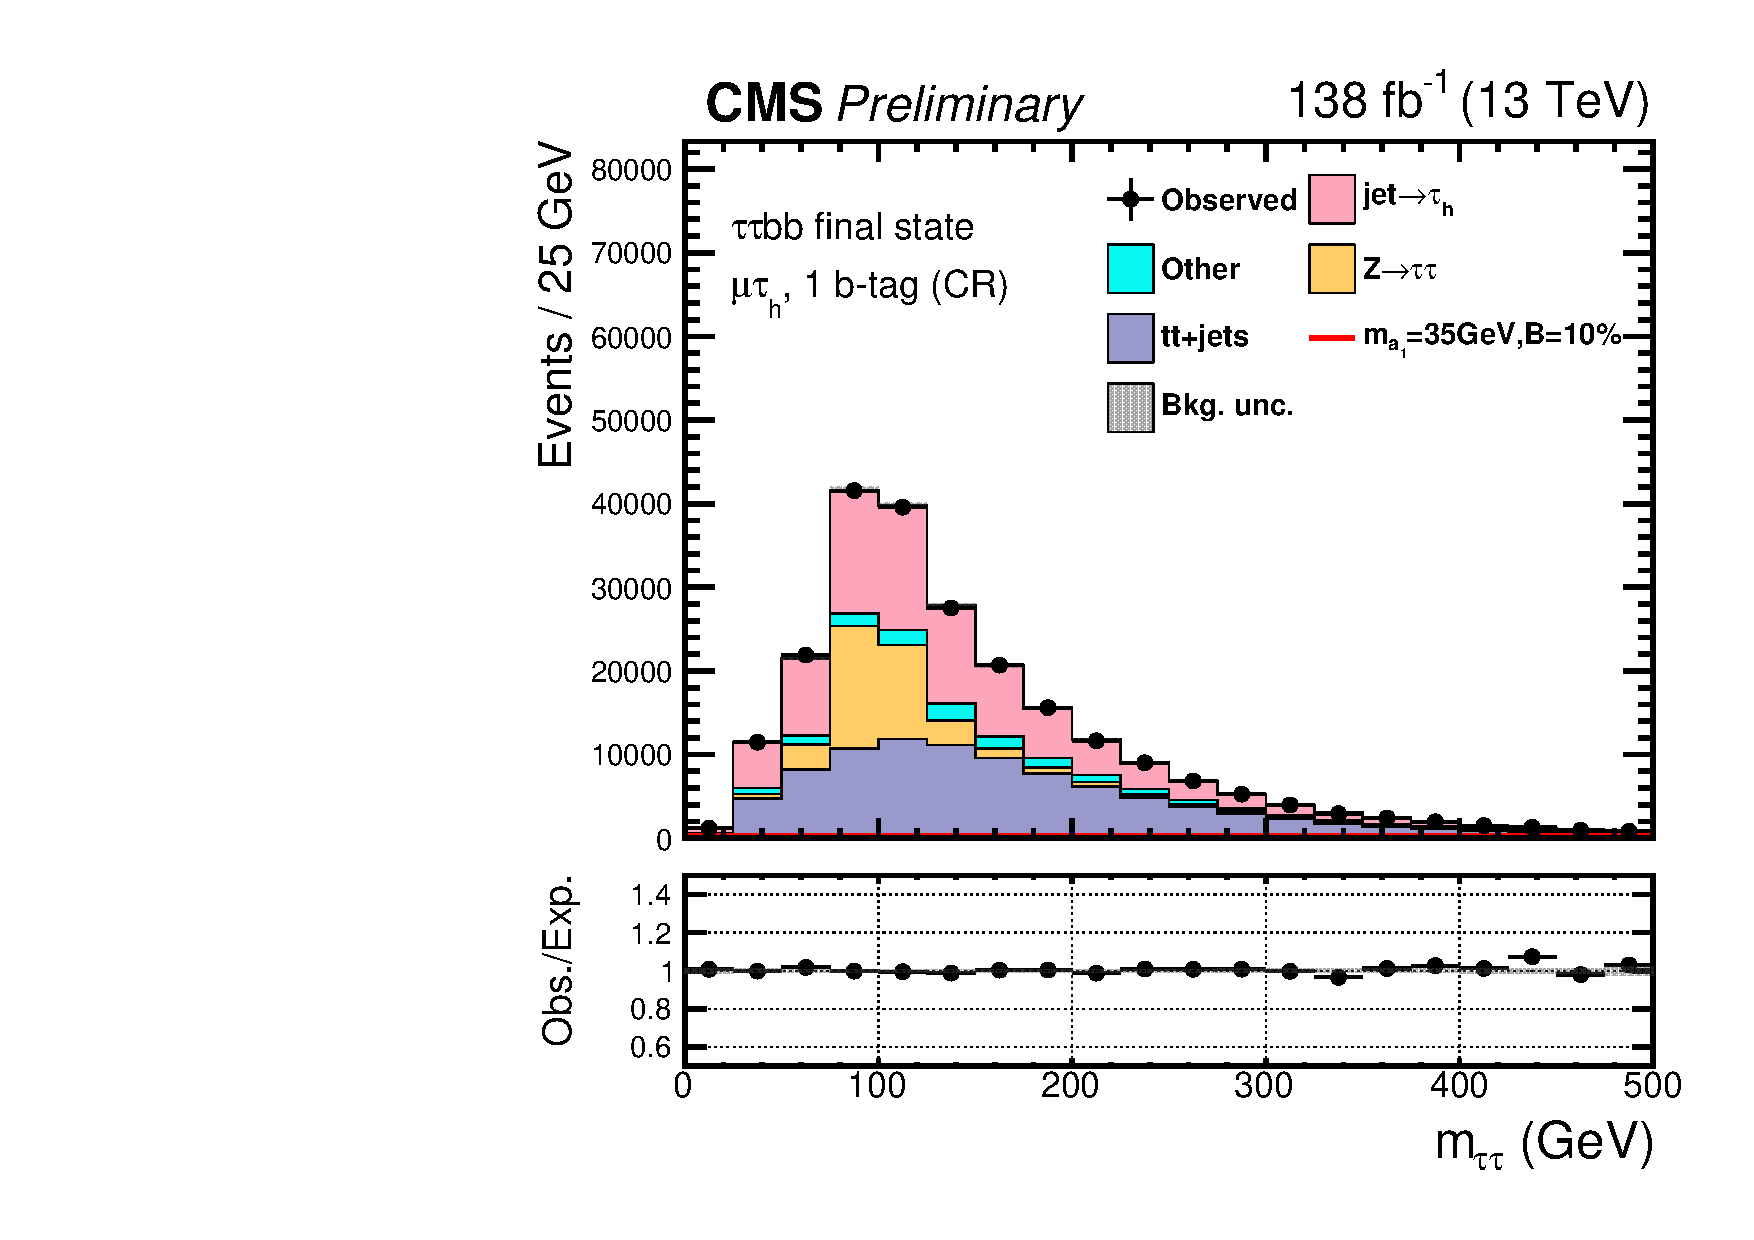
\includegraphics[width=0.32\textwidth]{figures/ch-10-results/mt_all_4_post_prelim-yes.pdf}
        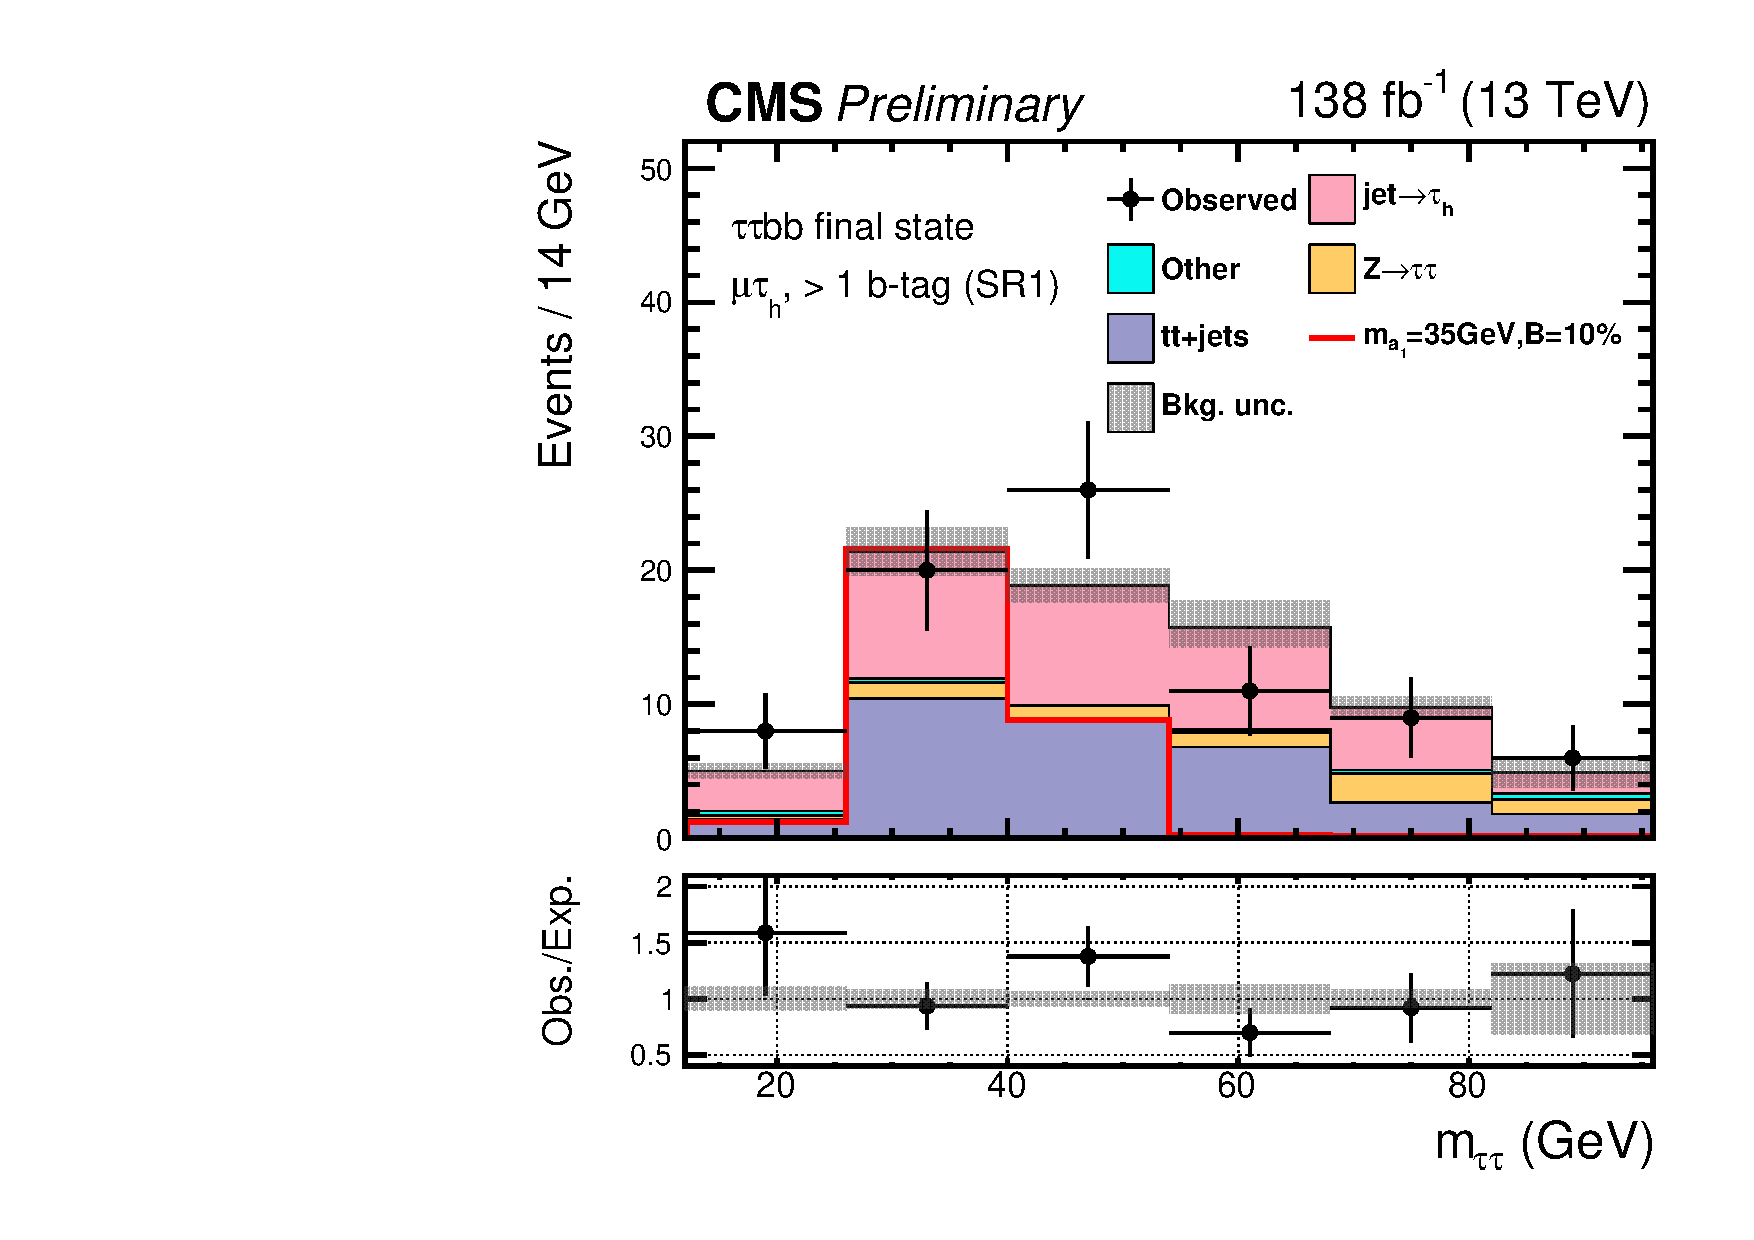
\includegraphics[width=0.32\textwidth]{figures/ch-10-results/mt_all_5_post_prelim-yes.pdf}
        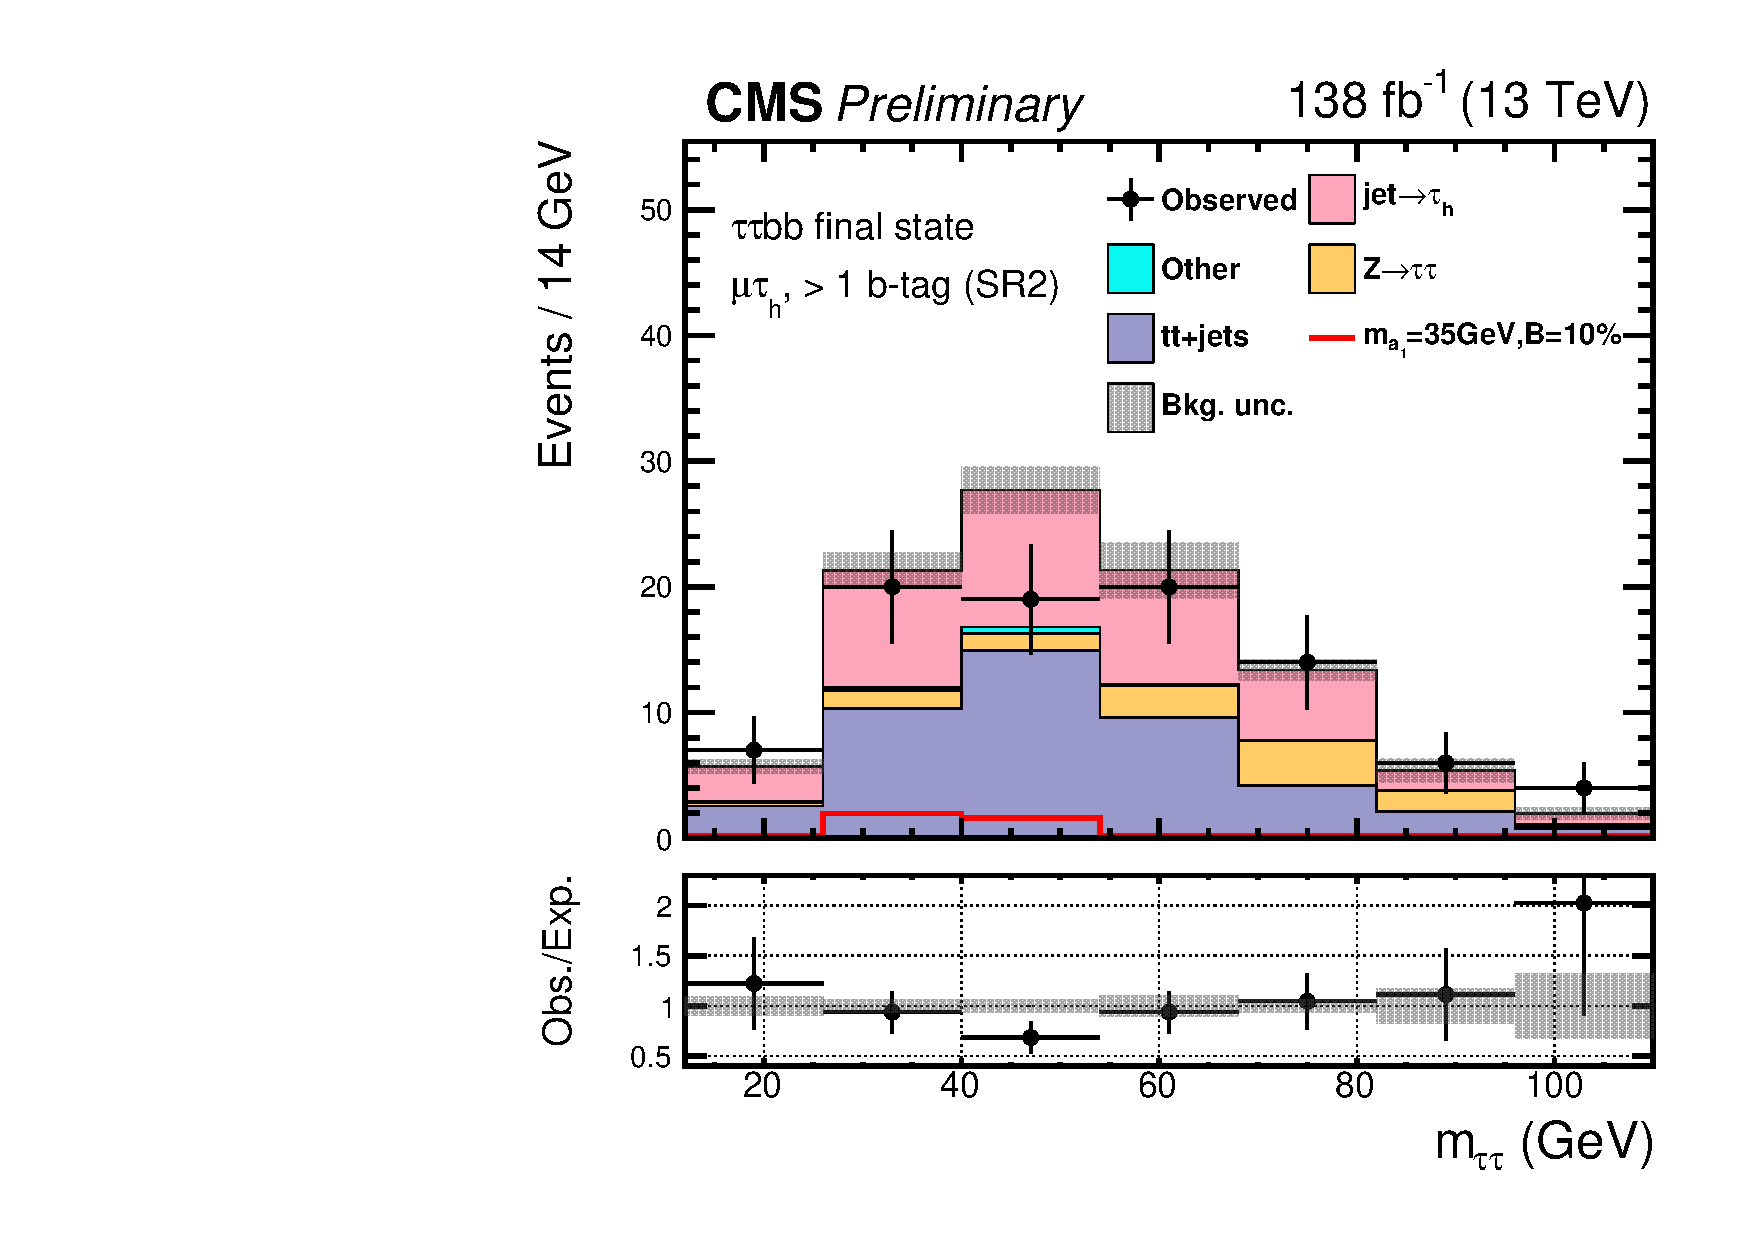
\includegraphics[width=0.32\textwidth]{figures/ch-10-results/mt_all_6_post_prelim-yes.pdf}\\
        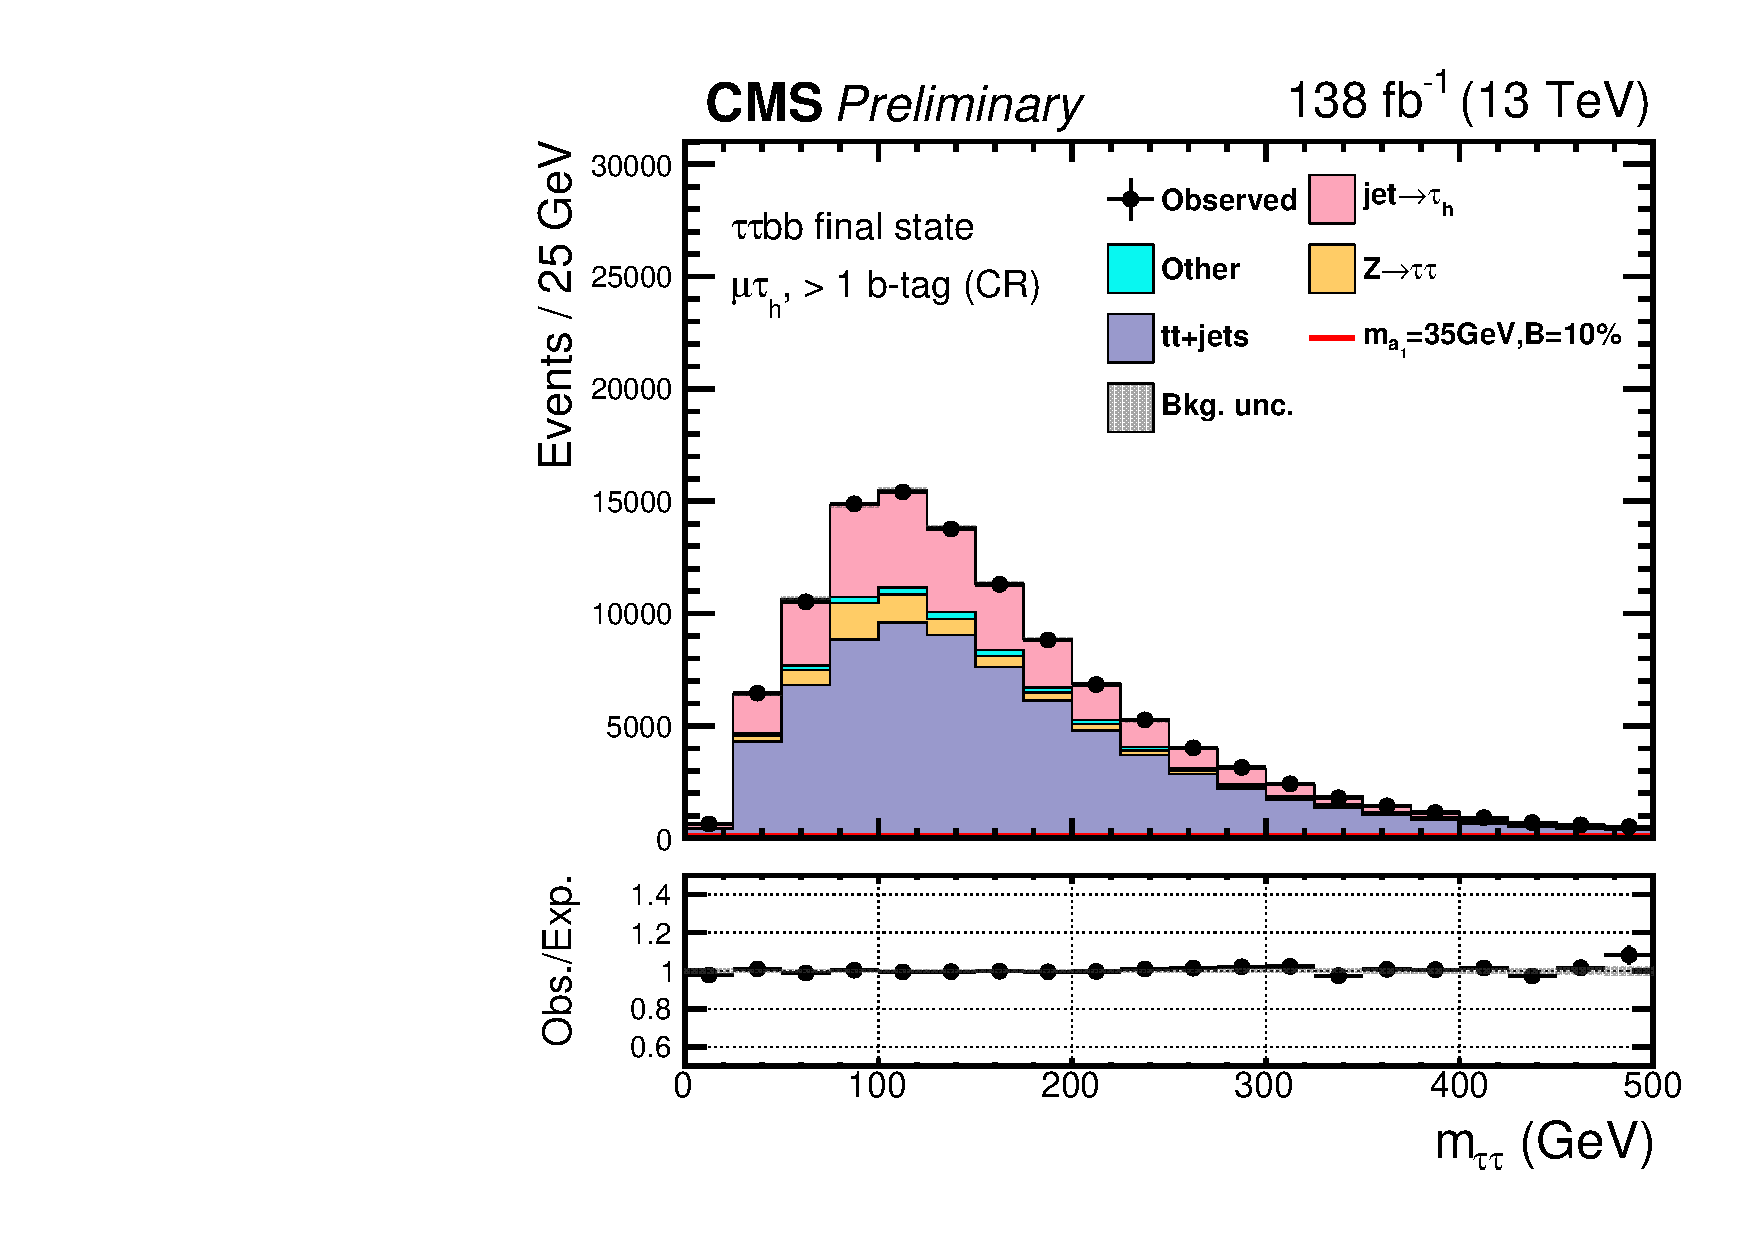
\includegraphics[width=0.32\textwidth]{figures/ch-10-results/mt_all_7_post_prelim-yes.pdf}
    \end{center}
    \caption[Postfit final observed and expected $m_{\tau\tau}$ distributions in the $\mu\tau_{h}$ channel, for the 1 b-tag jet and 2 b-tag jet signal and control regions.]{Postfit final $m_{\tau\tau}$ observed and expected distributions, and the observed/expected ratios, in the $\mu\tau_{h}$ channel~\cite{CMS-AN-20-213}. Events are divided into the 1 b-tag jet signal regions (SR1, SR2, SR3) (\textit{top row}), 1 b-tag jet control region (\textit{middle row}), 2 b-tag jet signal regions (SR1, SR2) (\textit{middle row}), and lastly the 2 b-tag jet control region (CR) (\textit{bottom}). Statistical and systematic sources of uncertainties in the expected events are added in quadrature and labeled ``Bkg. unc" (\textit{shaded gray}). The dominant backgrounds in all categories are jets faking the $\tau_{h}$ leg (\textit{pink}), $Z \rightarrow \tau\tau$ (\textit{orange}), and $t\bar{t}$+jets (\textit{purple}). For illustrative purposes, the beyond-Standard Model signal yield from $h\rightarrow aa \rightarrow bb\tau\tau$ is shown for the pseudoscalar mass hypothesis $m_a = 35$ GeV, assuming a branching fraction $B(h \rightarrow aa \rightarrow bb\tau\tau) = 10\%$ (\textit{red line}).}
    \label{fig:results_mtt_postfit_mtall}
\end{figure}

\begin{figure}[ht]
    \begin{center}
        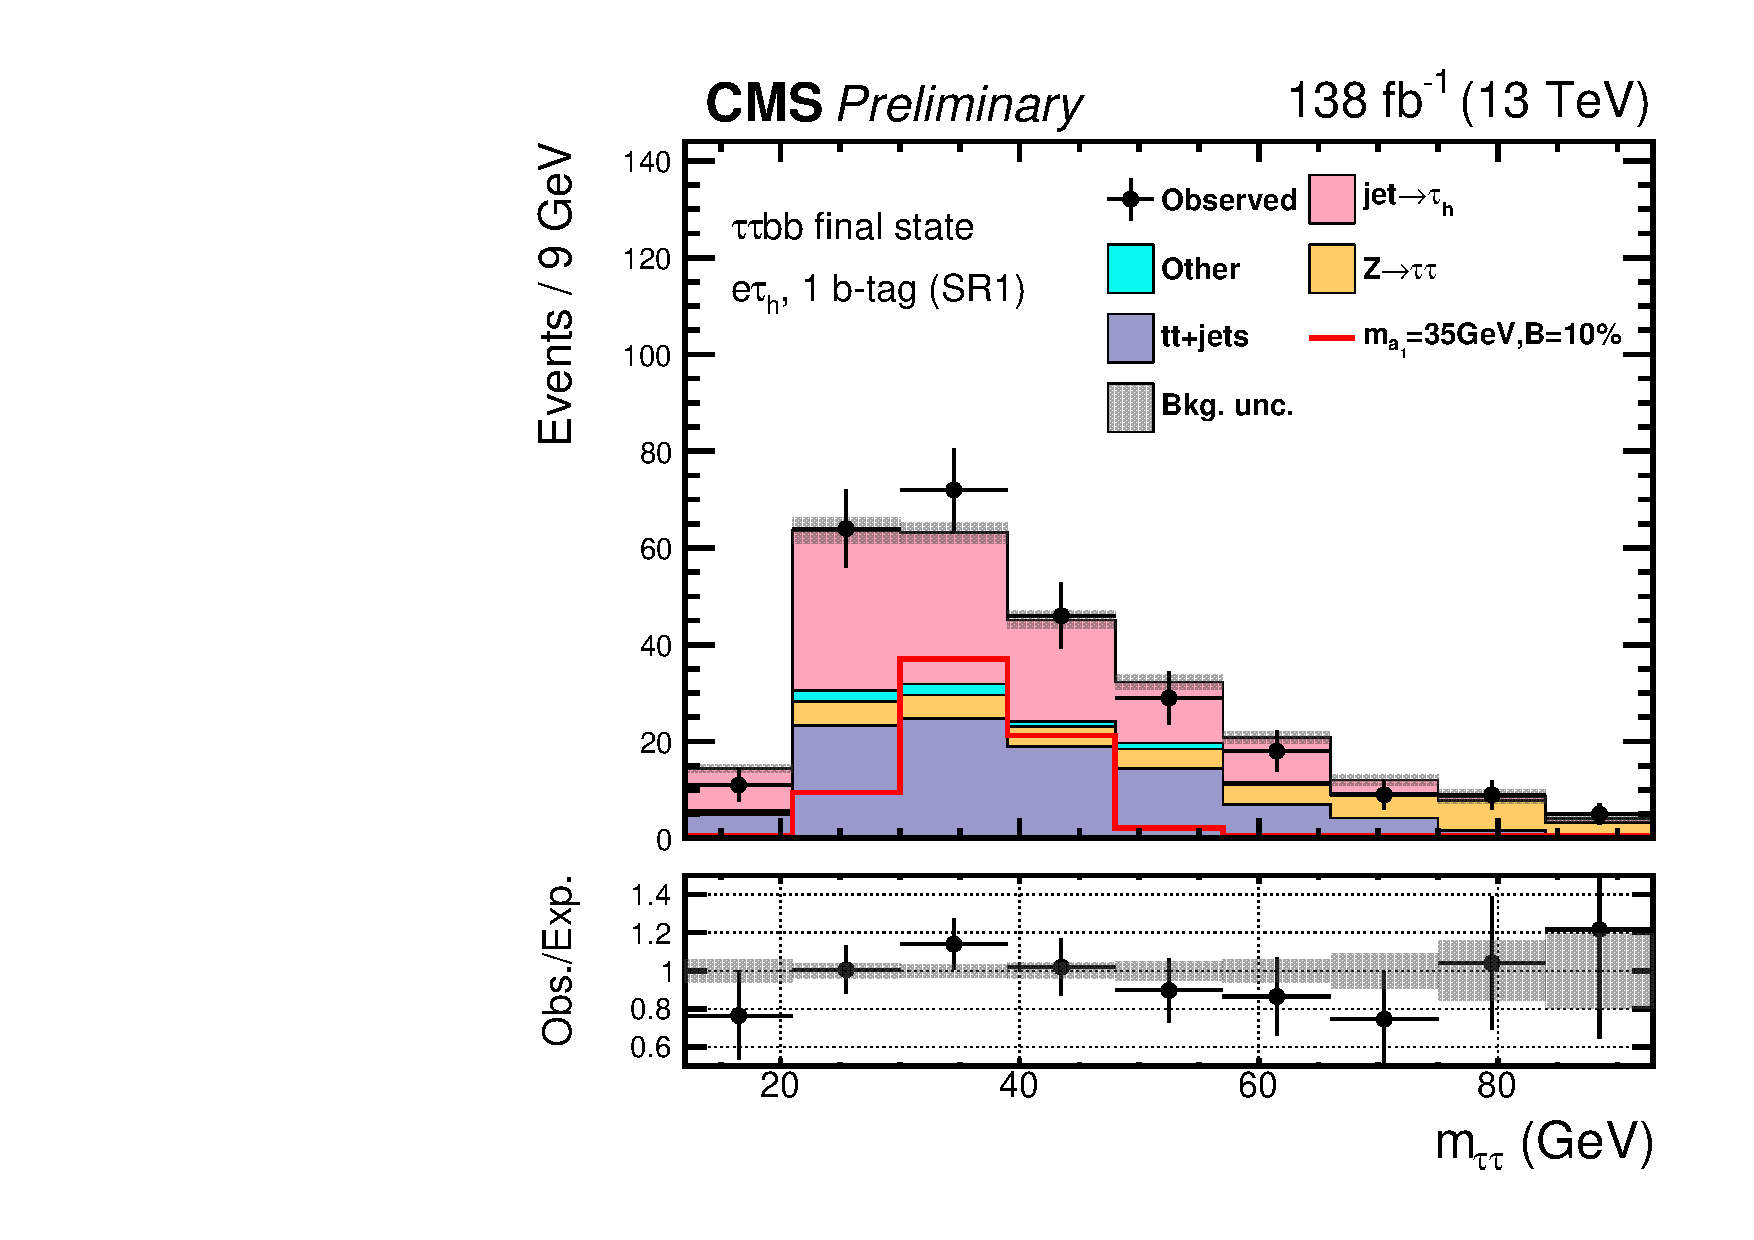
\includegraphics[width=0.32\textwidth]{figures/ch-10-results/et_all_1_post_prelim-yes.pdf}
        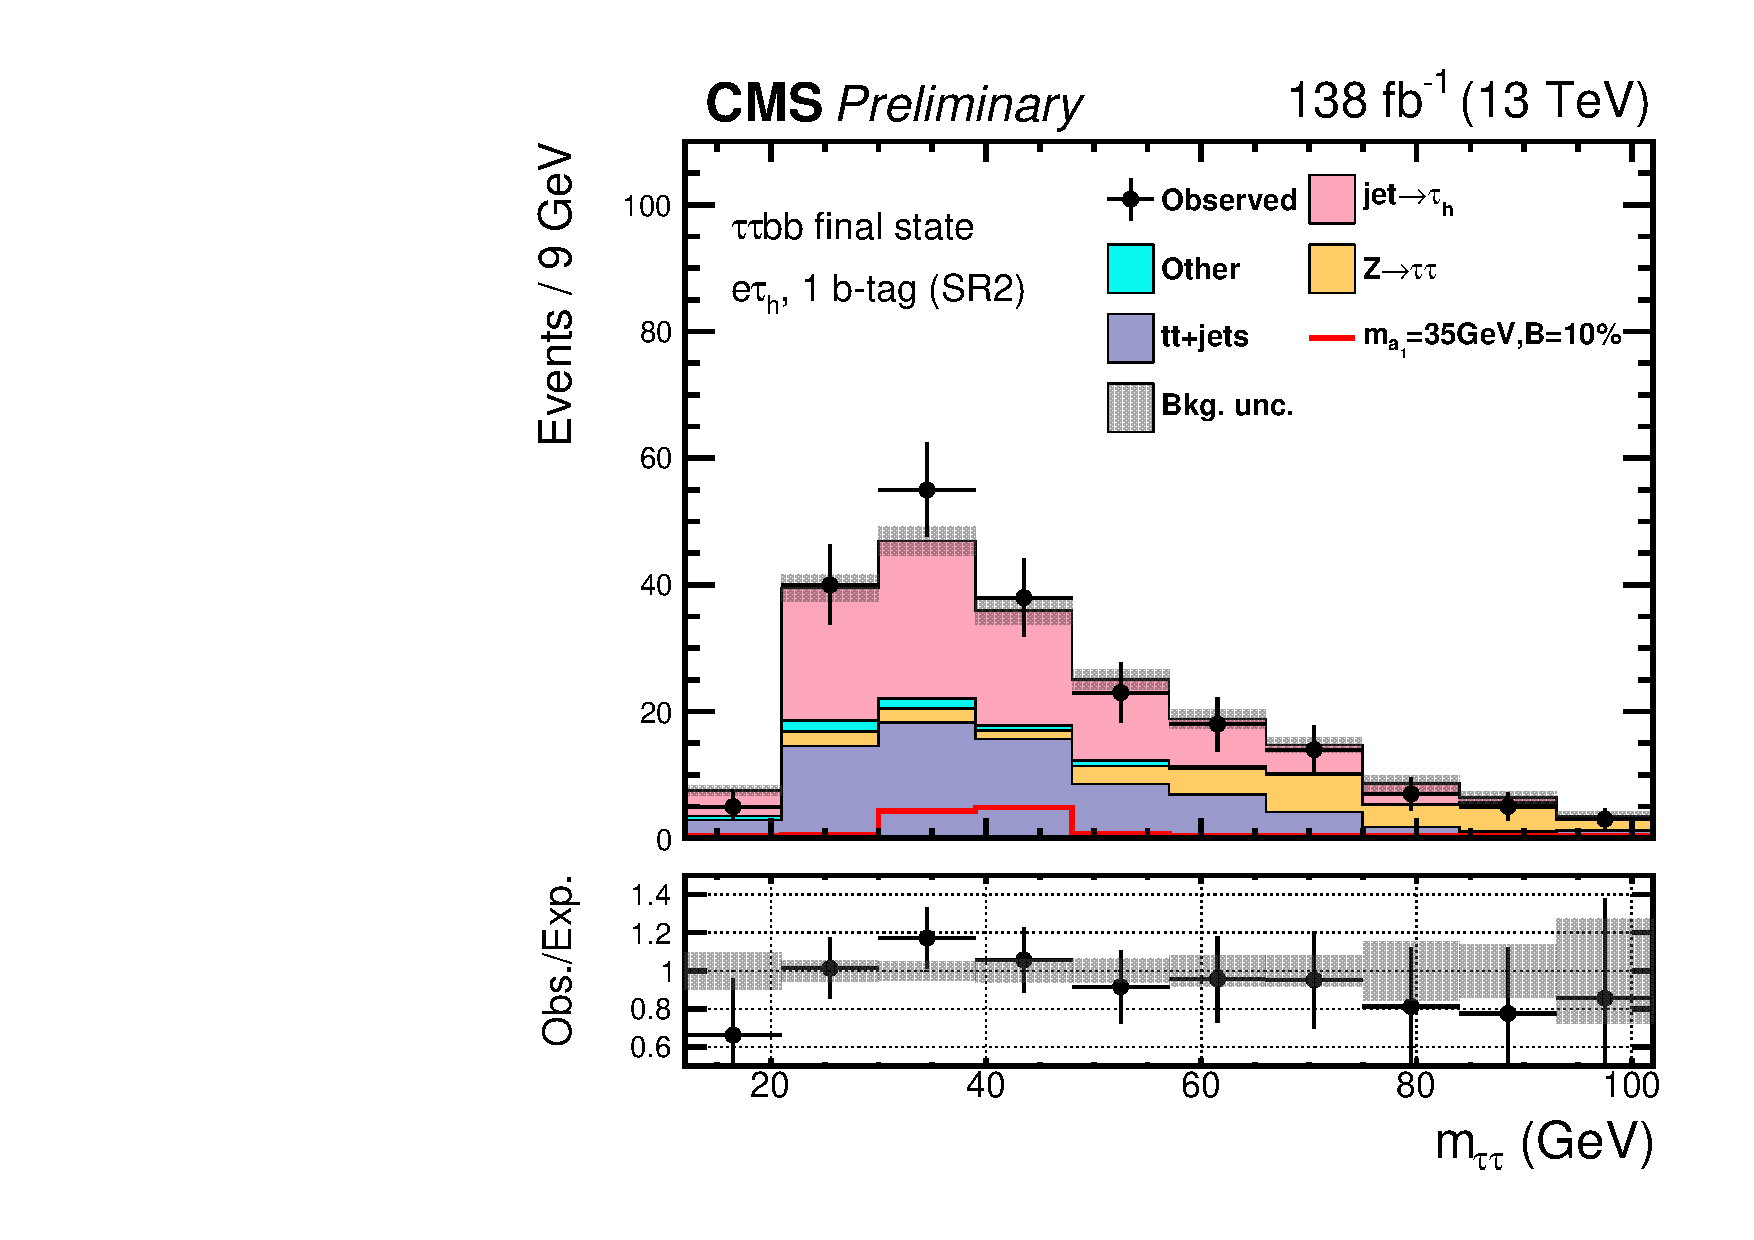
\includegraphics[width=0.32\textwidth]{figures/ch-10-results/et_all_2_post_prelim-yes.pdf}
        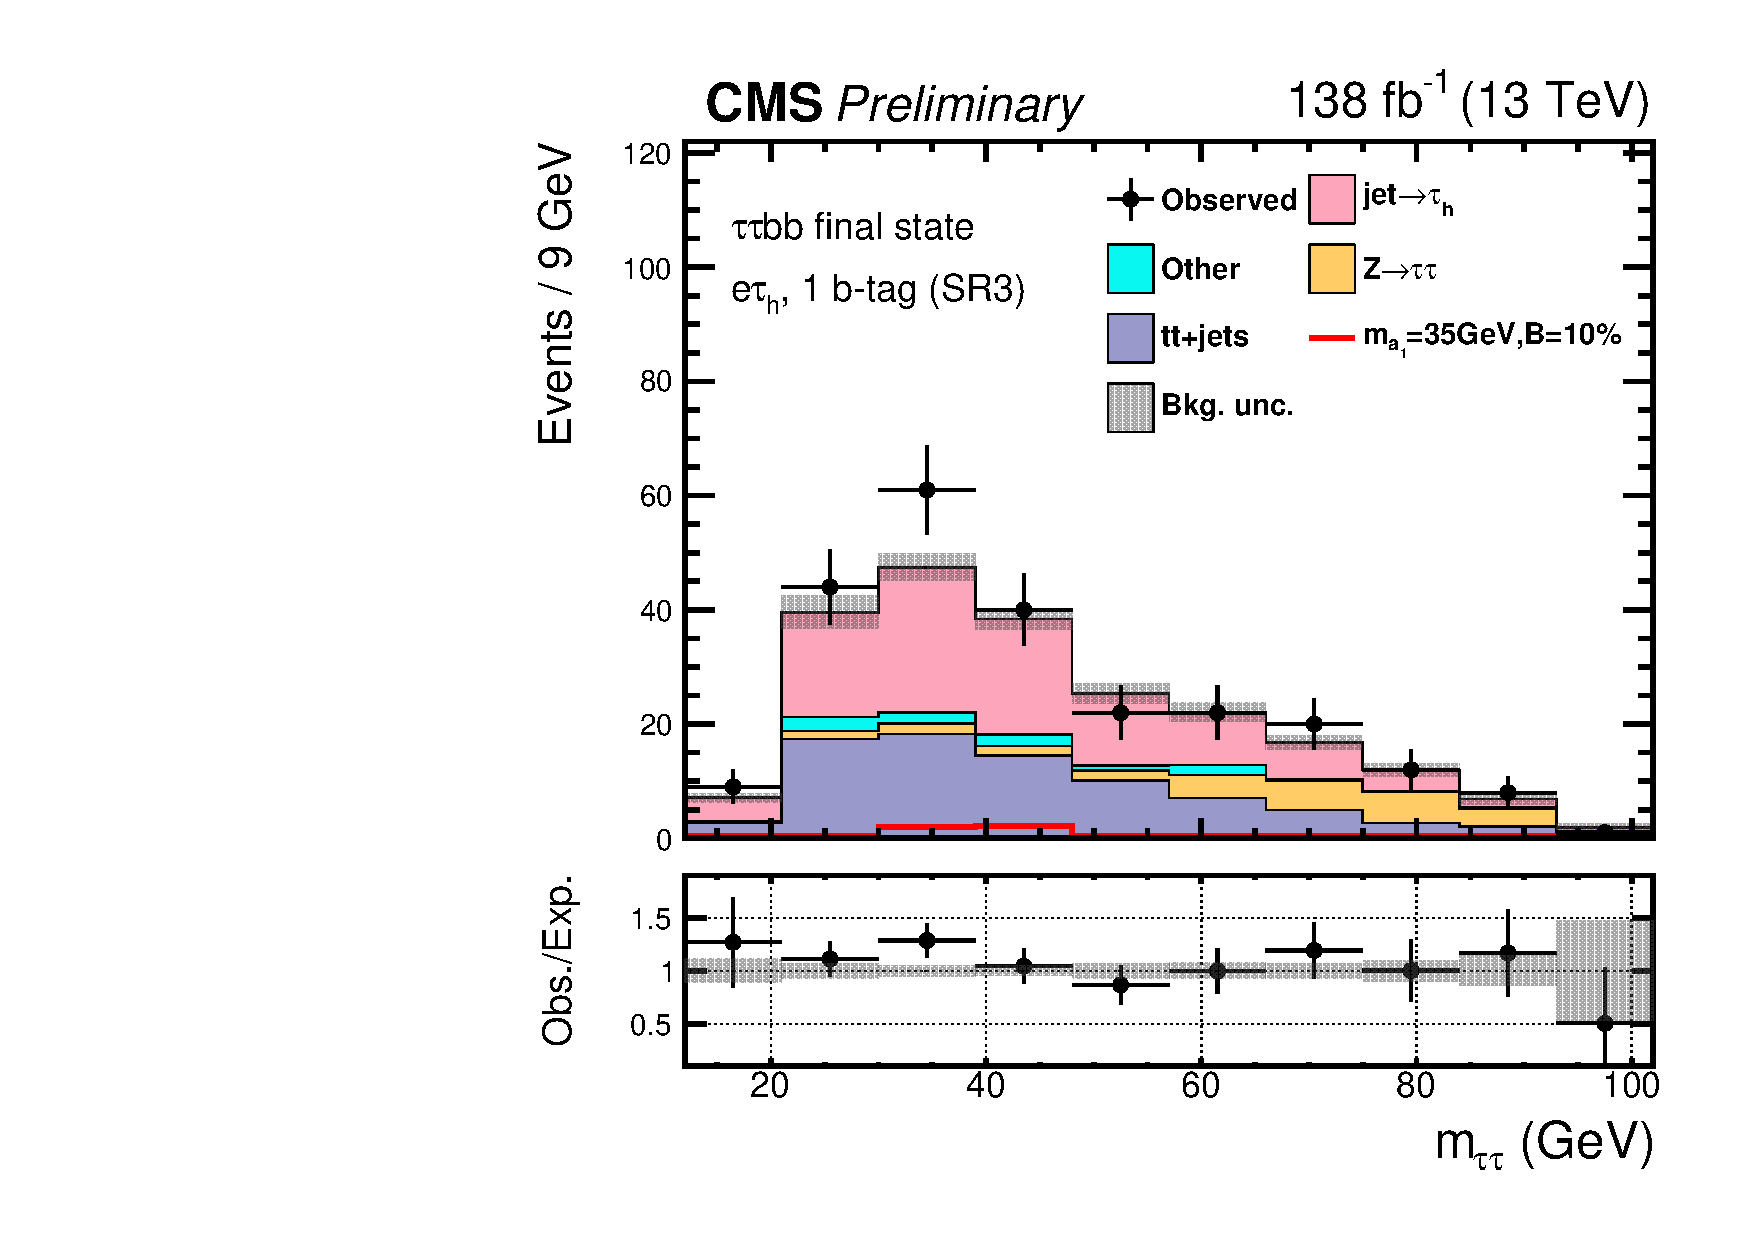
\includegraphics[width=0.32\textwidth]{figures/ch-10-results/et_all_3_post_prelim-yes.pdf}\\
        \includegraphics[width=0.32\textwidth]{figures/ch-10-results/et_all_4_post_prelim-yes.pdf}
        \includegraphics[width=0.32\textwidth]{figures/ch-10-results/et_all_5_post_prelim-yes.pdf}
        \includegraphics[width=0.32\textwidth]{figures/ch-10-results/et_all_6_post_prelim-yes.pdf}
    \end{center}
    \caption[Postfit final observed and expected $m_{\tau\tau}$ distributions in the $e\tau_{h}$ channel, for the 1 b-tag jet and 2 b-tag jet signal and control regions.]{Postfit final observed and expected $m_{\tau\tau}$ distributions, and the observed/expected ratios, in the $e\tau_{h}$ channel~\cite{CMS-AN-20-213}. Events are divided into the 1 b-tag jet signal regions (SR1, SR2, SR3) (\textit{top row}), the 1 b-tag jet control region (CR) (\textit{bottom row}), and 2 b-tag jet signal region (SR) and control region (CR) (\textit{bottom row}). Statistical and systematic sources of uncertainties in the expected events are added in quadrature and labeled ``Bkg. unc" (\textit{shaded gray}). In this channel, the dominant backgrounds are jets faking the $\tau_{h}$ leg (\textit{pink}), $Z \rightarrow \tau\tau$ (\textit{orange}), and $t\bar{t}$+jets (\textit{purple}). For illustrative purposes, the beyond-Standard Model signal yield from $h\rightarrow aa \rightarrow bb\tau\tau$ is shown for the pseudoscalar mass hypothesis $m_a = 35$ GeV, assuming a branching fraction $B(h \rightarrow aa \rightarrow bb\tau\tau) = 10\%$ (\textit{red line}).}
    \label{fig:results_mtt_postfit_etall}
\end{figure}

\begin{figure}[ht]
    \begin{center}
        \includegraphics[width=0.32\textwidth]{figures/ch-10-results/em_all_1_post_prelim-yes.pdf}
        \includegraphics[width=0.32\textwidth]{figures/ch-10-results/em_all_2_post_prelim-yes.pdf}
        \includegraphics[width=0.32\textwidth]{figures/ch-10-results/em_all_3_post_prelim-yes.pdf}\\
        \includegraphics[width=0.32\textwidth]{figures/ch-10-results/em_all_4_post_prelim-yes.pdf}
        \includegraphics[width=0.32\textwidth]{figures/ch-10-results/em_all_5_post_prelim-yes.pdf}
        \includegraphics[width=0.32\textwidth]{figures/ch-10-results/em_all_6_post_prelim-yes.pdf}\\
        \includegraphics[width=0.32\textwidth]{figures/ch-10-results/em_all_7_post_prelim-yes.pdf}
    \end{center}
    \caption[Postfit final observed and expected $m_{\tau\tau}$ distributions in the $e\mu$ channel.]{Postfit final observed and expected $m_{\tau\tau}$ distributions, and the observed/expected ratios, in the $e\mu$ channel~\cite{CMS-AN-20-213}. Events are divided into the 1 b-tag jet signal regions (SR1, SR2, and SR3) (\textit{top row}), 1 b-tag jet control region (CR) (\textit{middle row}), 2 b-tag jet signal regions (SR1 and SR2) (\textit{middle row}), and 2 b-tag jet control region (CR) (\textit{bottom row}). Statistical and systematic sources of uncertainties in the expected events are added in quadrature and labeled ``Bkg. unc" (\textit{shaded gray}). The $t\bar{t}$+jets process(\textit{purple}) is a major background, and in the signal regions the QCD multijet (\textit{pink}) is also a major background. For illustrative purposes, the beyond-Standard Model signal yield from $h\rightarrow aa \rightarrow bb\tau\tau$ is shown for the pseudoscalar mass hypothesis $m_a = 35$ GeV, assuming a branching fraction $B(h \rightarrow aa \rightarrow bb\tau\tau) = 10\%$ (\textit{red line}).}
    \label{fig:results_mtt_postfit_emall}
\end{figure}


The 95\% CL expected and observed exclusion limits on the signal strength of the branching fraction $B(h \rightarrow aa \rightarrow bb\tau\tau)$ as a function of the pseudoscalar mass $m_a$ ranging from 12 GeV to 60 GeV, are shown for the three $\tau\tau$ channels and all three channels combined in Fig. \ref{fig:results_limits}. The limits are shown as percentages and normalized to the production cross-section of the Standard Model Higgs boson. No excess of events above the Standard Model expectations is observed. In the limits for the three $\tau\tau$ channels combined, expected (observed) limits range from 1.4 to 5.6\% (1.7 to 7.6\%) for pseudoscalar masses between 12 and 60 GeV.


The $e\mu$ channel is the only channel that has signal sensitivity to the $m_a = 12$ GeV pseudoscalar mass hypothesis, because the minimum required spatial separation $\Delta R = \sqrt{(\Delta \eta)^2 + (\Delta \phi)^2}$ between the two $\tau$ legs is smaller than the other two channels ($\Delta R < 0.3$ for $e\mu$, compared to $\Delta R < 0.4$ for the other two channels). This decreased $\Delta R$ requirement results in better signal acceptance for low mass signals for the $e\mu$ channel. The $\mu\tau_{h}$ and $e\tau_{h}$ channels are most sensitive to the intermediate mass points studied, since the analysis targets a resolved signature: at low mass points, the tau legs are boosted, and at high mass points, the $m_{\tau\tau}$ distributions in signal have larger overlap with background distributions. In the combination of the three $\tau\tau$ channels, the limit for $m_a = 12$ GeV comes only from the $e\mu$ channel, and the best sensitivity is attained at intermediate mass points around $m_a = 20$ GeV to 45 GeV.


\begin{figure}[h!]
    \begin{center}
        \includegraphics[width=0.45\textwidth]{figures/ch-10-results/Limit_mt_prelim.pdf}
        \includegraphics[width=0.45\textwidth]{figures/ch-10-results/Limit_et_prelim.pdf}\\
        \includegraphics[width=0.45\textwidth]{figures/ch-10-results/Limit_em_prelim.pdf}
        \includegraphics[width=0.45\textwidth]{figures/ch-10-results/Limit_all_prelim.pdf}
    \end{center}
    \caption[Observed 95\% CL exclusion limits (\textit{black, solid lines}) and expected 95\% CL and 68\% CL limits (\textit{shaded yellow and green}) on the branching fraction B($h\rightarrow aa\rightarrow bb\tau\tau$) in percentages, assuming the Standard Model production for the 125\GeV Higgs ($h$). Limits are shown for the $\mu\tau_{h}$ channel (\textit{top left}), the $e\tau_{h}$ channel (\textit{top right}), and the $e\mu$ channel (\textit{bottom left}), and lastly the combination of all three channels (\textit{bottom right}) The dataset corresponds to 138 fb$^{-1}$ of data collected in the years 2016-2018 at a center-of-mass energy 13 TeV.]{Observed 95\% CL exclusion limits (\textit{black, solid lines}) and expected 95\% CL and 68\% CL limits (\textit{shaded yellow and green}) on the branching fraction B($h\rightarrow aa\rightarrow bb\tau\tau$) in percentages, assuming the Standard Model production for the 125\GeV Higgs ($h$). Limits are shown for the $\mu\tau_{h}$ channel (\textit{top left}), the $e\tau_{h}$ channel (\textit{top right}), and the $e\mu$ channel (\textit{bottom left}), and lastly the combination of all three channels (\textit{bottom right})~\cite{CMS-AN-20-213}. The dataset corresponds to 138 fb$^{-1}$ of data collected in the years 2016-2018 at a center-of-mass energy 13 TeV. Only the $e\mu$ channel has sensitivity to the mass hypothesis $m_a = 12$ GeV. The best sensitivity is attained at intermediate mass points.}
    \label{fig:results_limits}
\end{figure}

To set limits on the branching fraction of the 125\GeV Higgs to the two pseudoscalars, $B(h \rightarrow aa)$, we interpret the results in four types of 2HDM+S, which were introduced in Section \ref{section:theory-2HDM}. In 2HDM+S, the theorized branching fraction of the pseudoscalars depends on the 2HDM+S model type, the pseudoscalar mass $m_a$, and the ratio of the two Higgs doublets' vacuum expectation values $\tan\beta$. In Type I models, the branching fraction is independent of $\tan\beta$, while in Types II, III, and IV, it is a function of $m_a$ and $\tan\beta$. Limits for the $bb\tau\tau$ final state as a function of $m_a$ for 2HDM+S Type I (valid for all $\tan\beta$ values), Type II with $\tan\beta = 2.0$, Type III with $\tan\beta = 2.0$, and Type IV with $\tan\beta = 0.6$ are overlaid and shown in Fig. \ref{fig:bbtautau_only_limits}.


\section{Combination with \texorpdfstring{$bb\mu\mu$}{bbmumu} final state}
\label{section:combination-procedure-with-bbmumu}
Results from this analysis for the $h \rightarrow aa \rightarrow bb\tau\tau$ final state are combined with the analysis for the $h \rightarrow aa \rightarrow bb\mu\mu$ final state~\cite{CMS-AN-21-058-bbmumu}. While the predicted branching ratio for $aa \rightarrow bb\mu\mu$ is comparatively small, the $bb\mu\mu$ final state has competitive results due to the excellent di-muon resolution measured by CMS. The $bb\mu\mu$ analysis uses an unbinned fit to the data using the di-muon mass $m_{\mu\mu}$ distribution. Details can be found in~\cite{CMS-AN-21-058-bbmumu}.

Combining the results is possible since the $bb\tau\tau$ analysis explicitly rejects events with extra leptons, so there is no overlap between the events studied in the $bb\tau\tau$ analysis and the $bb\mu\mu$ analysis. In the statistical combination, several systematic uncertainties are treated as correlated: the integrated luminosity normalization, the b-tagging scale factor, the scale factors related to muon reconstruction, identification, and trigger efficiencies, the inefficiency in the ECAL trigger readout, and the theoretical uncertainties related to signal modeling.

Since the results in both final states are statistically limited, the combination benefits from the additional data. For $m_a = 35$ GeV, all systematic uncertainties amount to around 6\% of the total uncertainty, with the dominant systematic uncertainties coming from jet energy systematics in the $bb\mu\mu$ final state, theoretical uncertainties in the signal, and uncertainties in the QCD multijet backgrounds in the $e\mu$ channel of the $bb\tau\tau$ final state.

The mass distributions of the di-muon and di-tau objects ($m_{\mu\mu}$ and $m_{\tau\tau}$) are compared to the data in a combined maximum likelihood fit to derive upper limits on $B(h\rightarrow aa)$. The observed limits at 95\% CL on $B(h \rightarrow aa)$ for different 2HDM+S scenarios, are shown for the search for $h \rightarrow aa \rightarrow bb\mu\mu$ in Fig. \ref{fig:bbmumu_only_limits}, and the combined analyses $h \rightarrow aa \rightarrow bb\ell\ell$ in Fig. \ref{fig:results_limits_combined}. 

\begin{figure}[ht]
  \begin{subfigure}{0.45\textwidth}
    \includegraphics[width=1.0\textwidth]{figures/ch-10-results/HAA_bbtt_all_prelim.pdf}
    \caption{$bb\tau\tau$ final state.}
    \label{fig:bbtautau_only_limits}
\end{subfigure}
\hfill
\begin{subfigure}{0.45\textwidth}
    \includegraphics[width=1.0\textwidth]{figures/ch-10-results/HAA_bbmm_all_prelim.pdf}
      \caption{$bb\mu\mu$ final state.}
      \label{fig:bbmumu_only_limits}
  \end{subfigure}
  \caption[Observed 95\% CL upper limits on B$(h \rightarrow aa)$ in \%, for the $bb\tau\tau$ final state (\textit{left}) and $bb\mu\mu$ final state (\textit{right}) using the full Run 2 integrated luminosity of 138 fb$^{-1}$ in 2HDM+S type I (\textit{blue}), type II with $\tan\beta = 2.0$ (\textit{orange dashed}), type III with $\tan\beta = 2.0$ (\textit{dotted green}), and type IV with $\tan\beta = 0.6$ (\textit{red dashed}).]{Observed 95\% CL upper limits on B$(h \rightarrow aa)$ in \%, for the $bb\tau\tau$ final state (\textit{left}) and $bb\mu\mu$ final state (\textit{right}) using the full Run 2 integrated luminosity of 138 fb$^{-1}$ in 2HDM+S type I (\textit{blue}), type II with $\tan\beta = 2.0$ (\textit{orange dashed}), type III with $\tan\beta = 2.0$ (\textit{dotted green}), and type IV with $\tan\beta = 0.6$ (\textit{red dashed})~\cite{CMS-AN-20-213}. Linear interpolation is used between points in the graphs. The $\tan\beta$ values chosen here correspond to the most stringent limits in each model.}
  \label{fig:results_limits_bbtautau_bbmumu_separate}
\end{figure}

Exclusion limits in a two-dimensional plane as a function of $\tan\beta$ and $m_{a}$ are set for 2HDM+S Types II, III, and IV in Fig. \ref{fig:results_limits_combined_2D}. The most stringent constraints are observed for 2HDM+S type III because of large branching fractions predicted in theory, with predicted branching fractions between 0.47 and 0.42 for $\tan\beta = 2.0$ and values of $m_{a}$ between 15 and 60 GeV, compared to the observed 95\% CL upper limits which are between 0.08 and 0.03. For 2HDM+S type IV, the predicted branching fractions from theory are between 0.26 and 0.20 for $\tan\beta = 0.6$ for values of $m_{a}$ between 15 and 60 GeV, and the 95\% CL observed upper limits are between 0.12 and 0.05.  

  \begin{figure}[h!]
    \begin{center}
      \includegraphics[width=0.6\textwidth]{figures/ch-10-results/HAA_comb_all_prelim.pdf}
    \end{center}
    \caption[Observed 95\% CL upper limits on the branching fraction of the 125\GeV Higgs boson to two pseudoscalars, $B(h\to aa)$, in percentages, as a function of the pseudoscalar mass $m_a$, in 2HDM+S type I (\textit{blue}), type II with $\tan\beta = 2.0$ (\textit{orange dashed}), type III with $\tan\beta = 2.0$ (\textit{dotted green}), and type IV with $\tan\beta = 0.6$ (\textit{red dashed}), for the combination of $bb\mu\mu$ and $bb\tau\tau$ channels using the full Run 2 integrated luminosity of 138 fb$^{-1}$.]{Observed 95\% CL upper limits on the branching fraction of the 125\GeV Higgs boson to two pseudoscalars, $B(h\to aa)$, in percentages, as a function of the pseudoscalar mass $m_a$, in 2HDM+S type I (\textit{blue}), type II with $\tan\beta = 2.0$ (\textit{orange dashed}), type III with $\tan\beta = 2.0$ (\textit{dotted green}), and type IV with $\tan\beta = 0.6$ (\textit{red dashed}), for the combination of $bb\mu\mu$ and $bb\tau\tau$ channels using the full Run 2 integrated luminosity of 138 fb$^{-1}$~\cite{CMS-AN-20-213}.}
      \label{fig:results_limits_combined}
  \end{figure}
  


\begin{figure}[h]
    \begin{center}
      \includegraphics[width=0.32\textwidth]{figures/ch-10-results/HAA_comb_II_prelim.pdf}
      \includegraphics[width=0.32\textwidth]{figures/ch-10-results/HAA_comb_III_prelim.pdf}
      \includegraphics[width=0.32\textwidth]{figures/ch-10-results/HAA_comb_IV_prelim.pdf}
    \end{center}
    \caption[Observed 95\% CL upper limits on $\mathcal{B}(h\to aa)$ in \%, for the combination of $bb\mu\mu$ and $bb\tau\tau$ channels using the full Run 2 integrated luminosity of 138 fb$^{-1}$ for Type II (\textit{left}), Type III (\textit{middle}), and Type IV (\textit{right}) 2HDM+S in the $\tan\beta$ vs. $m_a$ phase space.]{Observed 95\% CL upper limits on $\mathcal{B}(h\to aa)$ in \%, for the combination of $bb\mu\mu$ and $bb\tau\tau$ channels using the full Run 2 integrated luminosity of 138 fb$^{-1}$ for Type II (\textit{left}), Type III (\textit{middle}), and Type IV (\textit{right}) 2HDM+S in the $\tan\beta$ vs. $m_a$ phase space. The contours (\textit{dashed black}) correspond to branching fractions of 100\% and 16\%, where 16\% is the combined upper limit on Higgs boson to undetected particle decays from previous Run-2 results. All points inside the contour are allowed within that upper limit. Linear extrapolation has been used between different points on the figures~\cite{CMS-AN-20-213}.}
      \label{fig:results_limits_combined_2D}
  \end{figure}
  
The combined results from $h\rightarrow aa \rightarrow bb\ell\ell$ are compared with CMS results in other final states as a function of the pseudoscalar mass $m_a$: for 2HDM+S type I in Fig. \ref{fig:summary_plot_type_I}, type II with $\tan\beta = 2.0$ in Fig. \ref{fig:summary_plot_typeII_tan_beta_2p0}, and type III with $\tan\beta = 2.0$ in Fig. \ref{fig:summary_plot_typeIII_tan_beta_2p0}. In other scenarios, e.g. type III with $\tan\beta = 5.0$, more stringent limits are set by analyses in other final states, $\mu\mu\tau\tau$ in this case. Other summary plots for other model types and $\tan\beta$ values can be found at~\cite{twiki_2HDM+S_summary-plots}.


\begin{figure}[h]
    \begin{center}
      \includegraphics[width=0.6\textwidth]{figures/ch-10-results/summary_plot_full_run2_plot_BRaa_Type1.pdf}
    \end{center}
    \caption[Summary plot of current observed and expected 95\% CL limits on the branching ratio of the 125\GeV Higgs boson to two pseudoscalars, normalized to the Standard Model Higgs production cross-section, $\frac{\sigma(h)}{\sigma_{\text{SM}}} \times B(h \rightarrow aa)$, in the 2HDM+S type I scenario, obtained at CMS with data collected at 13 TeV.]{Summary plot of current 95\% limits on the branching ratio of the 125\GeV Higgs boson to two pseudoscalars, normalized to the Standard Model Higgs production cross-section, $\frac{\sigma(h)}{\sigma_{\text{SM}}} \times B(h \rightarrow aa)$ in the 2HDM+S type I scenario performed with data collected at 13 TeV~\cite{twiki_2HDM+S_summary-plots}. Results from different final states studied at CMS are overlaid on this figure: $\mu\mu\mu\mu$ (\textit{blue}), $\tau\tau\tau\tau$ (\textit{green}), boosted $2\mu 2\tau$ (\textit{red}), resolved $2\mu 2\tau$ (\textit{yellow}), $bbbb$ (\textit{magenta}), and the combined result for $\ell\ell bb$ ($\ell = \mu, \tau$) (\textit{purple}).}
      \label{fig:summary_plot_type_I}
  \end{figure}
  \begin{figure}[h]
    \begin{center}
      \includegraphics[width=0.6\textwidth]{figures/ch-10-results/summary_plot_full_run2_plot_BRaa_Type2_tanbeta2.pdf}
    \end{center}
    \caption[Summary plot of current observed and expected 95\% CL limits on the branching ratio of the 125\GeV Higgs boson to two pseudoscalars, normalized to the Standard Model Higgs production cross-section, $\frac{\sigma(h)}{\sigma_{\text{SM}}} \times B(h \rightarrow aa)$, in the 2HDM+S type II scenario with $\tan\beta = 2.0$, obtained at CMS with data collected at 13 TeV.]{Summary plot of current observed and expected 95\% CL limits on the branching ratio of the 125\GeV Higgs boson to two pseudoscalars, normalized to the Standard Model Higgs production cross-section, $\frac{\sigma(h)}{\sigma_{\text{SM}}} \times B(h \rightarrow aa)$, in the 2HDM+S type II scenario with $\tan\beta = 2.0$, obtained at CMS with data collected at 13 TeV~\cite{twiki_2HDM+S_summary-plots}. Results from different final states studied at CMS are overlaid on this figure: $\mu\mu\mu\mu$ (\textit{blue}), $\tau\tau\tau\tau$ (\textit{green}), boosted $2\mu 2\tau$ (\textit{red}), resolved $2\mu 2\tau$ (\textit{yellow}), $bbbb$ (\textit{magenta}), and the combined result for $\ell\ell bb$ ($\ell = \mu, \tau$) (\textit{purple}).}
      \label{fig:summary_plot_typeII_tan_beta_2p0}
  \end{figure}
  \begin{figure}[h]
    \begin{center}
      \includegraphics[width=0.6\textwidth]{figures/ch-10-results/summary_plot_full_run2_plot_BRaa_Type3_tanbeta2.pdf}
    \end{center}
    \caption[Summary plot of current observed and expected 95\% CL limits on the branching ratio of the 125\GeV Higgs boson to two pseudoscalars, normalized to the Standard Model Higgs production cross-section, $\frac{\sigma(h)}{\sigma_{\text{SM}}} \times B(h \rightarrow aa)$, in the 2HDM+S type III scenario with $\tan\beta = 2.0$, obtained at CMS with data collected at 13 TeV.]{Summary plot of current observed and expected 95\% CL limits on the branching ratio of the 125\GeV Higgs boson to two pseudoscalars, normalized to the Standard Model Higgs production cross section, $\frac{\sigma(h)}{\sigma_{\text{SM}}} \times B(h \rightarrow aa)$ in the 2HDM+S type-III scenario with $\tan\beta = 2.0$, obtained at CMS with data collected at 13 TeV~\cite{twiki_2HDM+S_summary-plots}. Results from different final states studied at CMS are overlaid on this figure: $\mu\mu\mu\mu$ (\textit{blue}), $\tau\tau\tau\tau$ (\textit{green}), boosted $2\mu 2\tau$ (\textit{red}), resolved $2\mu 2\tau$ (\textit{yellow}), $bbbb$ (\textit{magenta}), and the combined result for $\ell\ell bb$ ($\ell = \mu, \tau$) (\textit{purple}).}
      \label{fig:summary_plot_typeIII_tan_beta_2p0}
  \end{figure}
  


\chapter{Asymmetric exotic Higgs decays}
In this chapter, progress towards a search for exotic Higgs decays to two light scalars with unequal mass ($h \rightarrow a_1 a_2$) final states with bottom quarks and $\tau$ leptons is presented. To date, the asymmetric decay $h_{125} \rightarrow a_1 a_2$ has not been directly searched for at the CMS experiment.

\section{Signal masses}
As discussed in Section \ref{section:theory-TRSM}, $h \rightarrow a_1 a_2$ can result in a ``cascade" decay if one of the scalars, $a_2$ is sufficiently heavy ($m_{a_2} > 2m_{a_1}$). The ``non-cascade" case is where the light scalars decay directly to Standard Model particles. 

The mass hypotheses (mass points) $(m_{a_1}, m_{a_2})$ studied here are:
\begin{itemize}
    \item \textit{Cascade mass points:} (15, 30), (15, 40), (15, 50), (15, 60), (15, 70), (15, 80), (15, 90), (15, 100), (15, 110), (20, 40), (20, 50), (20, 60), (20, 70), (20, 80), (20, 90), (20, 100), (30, 60), (30, 70), (30, 80), and (30, 90) GeV
    \item \textit{Non-cascade mass points:} (15, 20), (15, 30), (20, 30), (20, 40), (30, 40), (30, 50), (30, 60), (40, 50), (40, 60), (40, 70), (40, 80), (50, 60), and (50, 70) GeV
\end{itemize}
Samples were produced using the MadGraph5\_aMCatNLO event generator, for each signal mass point in the gluon-gluon fusion (ggF) and vector boson fusion (VBF) production modes of the 125 GeV Higgs boson. In the sample generation, the decays of $a$ to Standard Model particles were specified to be decays to bottom quarks or $\tau$ leptons.


\section{Cascade scenario signal studies}
Studies of the signal phenomenology in the cascade scenario were performed to determine the viability of the $4b2\tau$ and/or $2b4\tau$ channels. 

Cross sections and branching fractions of the $4b2\tau$ and $2b4\tau$ final states were compared using cross-section predictions provided by the authors of \cite{Robens:2019kga}. For an example mass point $m_{a_2} = 80$ GeV, $m_{a_1} = 30$ GeV, the branching fractions to $4b2\tau$ is ten times larger than $2b4\tau$: $B(h \rightarrow a_1 a_2 \rightarrow 3 a_1 \rightarrow 4b2\tau) = 0.00857$, vs. $B(h \rightarrow a_1 a_2 \rightarrow 3 a_1 \rightarrow 2b4\tau) = 0.00068$. The $4b2\tau$ final state is chosen for this analysis.

In general the four b-jets have low $p_{T}$ at generator level, as illustrated for example mass points (100, 15) GeV and (40, 20) GeV in Fig. \ref{fig:overlay_cascade_b_jet_gen_pT}. The $p_{T}$ distribution of the sub-leading jet peaks at an energy below 20 GeV, with the third and fourth jets tending to have even softer energies.

An event category with three or more b-tag jets was determined to be infeasible due to low statistics in this category, due to the difficulties in reconstructing the third and fourth b jets which have very low transverse momenta $p_{T}$. Event categories with exactly 1 b-tag jet and $\geq 2$ b-tag jets will be used.

\begin{figure}[h]
    \centering
    \begin{subfigure}{0.45\textwidth}
        \includegraphics[width=1.0\textwidth]{figures/ch-11-asymmetric/Cascade_ggH_MA2-100_MA1-15_overlay}
    \end{subfigure}
    \hfill
    \begin{subfigure}{0.45\textwidth}
        \includegraphics[width=1.0\textwidth]{figures/ch-11-asymmetric/Cascade_ggH_MA2-40_MA1-20_overlay}
    \end{subfigure}  
    \caption{Generator-level b-jet transverse momenta $p_{T}$, for $h \rightarrow a_1 a_2$ cascade scenario in the $4b2\tau$ final state, for mass hypotheses $(m_{a_1}, m_{a_2}) = (100, 15)$ GeV (\textit{left}) and (40, 20) GeV (\textit{right}). In each plot the generator-level $p_{T}$ of the leading (\textit{black}), sub-leading (\textit{red}), third (\textit{blue}), and fourth (\textit{light green}) are overlaid.}
    \label{fig:overlay_cascade_b_jet_gen_pT}
\end{figure}


In the $4b2\tau$ final state, the possibility of the leading and sub-leading b-tag jets being sufficiently close in $\Delta R$ to require boosted jet reconstruction techniques was explored. In the $4b2\tau$ case, the two b-jets in the generated event that were spatially closest in $\Delta R$ were considered as one object. This two b-jet object was spatially matched in $\Delta R$ to the jets reconstructed with the standard AK4 algorithm which uses a cone size of $\Delta R = 0.4$. The quality of the $p_{T}$ resolution (computed as $(p_{T, \text{reconstructed}} - p_{T, \text{gen}})/ p_{T, \text{gen}}$) and closeness in distance $\Delta R$ of the reconstructed jet to the nearest generator-level jets, was seen to depend on the absolute and relative masses of the light scalars. The best (worst) performance occurred in samples with large (small) mass differences between the heavier scalar $a_2$ and the lighter scalar $a_1$, as illustrated for the mass hypotheses $(m_{a_1}, m_{a_2})$ (100, 15) GeV and (40, 20) GeV in Fig. \ref{fig:cascade_matching_to_AK4_jets}.


\begin{figure}[h]
    \centering
    \begin{subfigure}{0.45\textwidth}
        \includegraphics[width=1.0\textwidth]{figures/ch-11-asymmetric/Cascade_ggH_MA2-100_MA1-15_pt_resolution_ak4_leadingPair}
    \end{subfigure}
    \hfill
    \begin{subfigure}{0.45\textwidth}
        \includegraphics[width=1.0\textwidth]{figures/ch-11-asymmetric/Cascade_ggH_MA2-100_MA1-15_deltaR_ak4_leadingPair}
    \end{subfigure} \\
    \begin{subfigure}{0.45\textwidth}
        \includegraphics[width=1.0\textwidth]{figures/ch-11-asymmetric/Cascade_ggH_MA2-40_MA1-20_pt_resolution_ak4_leadingPair}
    \end{subfigure}
    \hfill
    \begin{subfigure}{0.45\textwidth}
        \includegraphics[width=1.0\textwidth]{figures/ch-11-asymmetric/Cascade_ggH_MA2-40_MA1-20_deltaR_ak4_leadingPair}
        % \caption{$\tau_{h}$ efficiency from $e\tau_{h}$ trigger.}
        % \label{fig:}
    \end{subfigure}     
    \caption{Distributions (arbitrary units) of transverse momentum $p_{T}$ resolution and $\Delta R$ between the two closest generator-level $b$ jets, treated as one object, and the nearest reconstructed AK4 jet, for two different $h\rightarrow a_1 a_2$ mass hypotheses $(m_{a_1}, m_{a_2}) = (100, 15)$ GeV (\textit{top left, top right}) and $(40, 20)$ GeV (\textit{bottom left, bottom right}) in the ggH production of the 125 GeV $h$. In the $(40, 20)$ GeV mass point, the longer $p_{T}$ resolution tail (\textit{bottom left}) indicates that the reconstructed jet underestimates the generator b-jets' energy, and the significant fraction of events with larger $\Delta R$ values (\textit{bottom right}) indicate worse matching.}
    \label{fig:cascade_matching_to_AK4_jets}
\end{figure}



\section{Current control plots for $\mu\tau_{h}$ channel}

The $\tau\tau$ states for the $h \rightarrow a_1 a_2$ to $4b2\tau$ analysis will be similar to those studied in $h\rightarrow aa \rightarrow bb\tau\tau$. For the $\mu\tau_{h}$ channel, histograms of the key kinematic variables are made for data and the sum of the expected backgrounds, which are estimated from Monte Carlo samples, embedded samples, and the data-driven method for estimating jets faking $\tau_{h}$ as described in Chapter \ref{chapter:ch-7:background-estimation}. Nominal values of the scale factors and event reweighing are applied, as described in Chapter \ref{chapter:ch-8:scale-factors-and-corrections}. The errors shown in the figures only include statistical errors and only several of the full set of systematic errors (only those associated with the lepton energy scales and $\tau_{h}$ identification efficiency, described in Sections \ref{sec:tau_energy_scale}, \ref{sec:muon_energy_scale}, and \ref{sec:tauh_id_efficiency}). 

The $p_{T}$, $\eta$, and $\phi$ of the leading muon and hadronic tau $\tau_{h}$, and the di-tau visible mass $m_{\text{vis}}$ and momentum $p_{T, \text{vis}}$, are shown in Fig. \ref{fig:nanoAOD_mutau_control_plots_leading_mutauh}. The $p_{T}$, $\eta$, and $\phi$ of the the leading and sub-leading b-tag jets, and the missing transverse energy magnitude and azimuthal direction, are shown in Fig. \ref{fig:nanoAOD_mutau_control_plots_btagjets_met_metphi}.

\begin{figure}[h]
    \centering
    \begin{subfigure}{0.45\textwidth}
        \includegraphics[width=1.0\textwidth]{figures/ch-11-asymmetric/mutau_pt_1.png}
    \end{subfigure}
    \hfill
    \begin{subfigure}{0.45\textwidth}
        \includegraphics[width=1.0\textwidth]{figures/ch-11-asymmetric/mutau_pt_2.png}
    \end{subfigure} \\
    \begin{subfigure}{0.45\textwidth}
        \includegraphics[width=1.0\textwidth]{figures/ch-11-asymmetric/mutau_eta_1.png}
    \end{subfigure}
    \hfill
    \begin{subfigure}{0.45\textwidth}
        \includegraphics[width=1.0\textwidth]{figures/ch-11-asymmetric/mutau_eta_2.png}
    \end{subfigure} \\   
    \begin{subfigure}{0.45\textwidth}
        \includegraphics[width=1.0\textwidth]{figures/ch-11-asymmetric/mutau_phi_1.png}
    \end{subfigure}
    \hfill
    \begin{subfigure}{0.45\textwidth}
        \includegraphics[width=1.0\textwidth]{figures/ch-11-asymmetric/mutau_phi_2.png}
    \end{subfigure} \\     
    \begin{subfigure}{0.45\textwidth}
        \includegraphics[width=1.0\textwidth]{figures/ch-11-asymmetric/mutau_m_vis.png}
    \end{subfigure}
    \hfill
    \begin{subfigure}{0.45\textwidth}
        \includegraphics[width=1.0\textwidth]{figures/ch-11-asymmetric/mutau_pt_vis.png}
    \end{subfigure} \\   
    \caption{Kinematic properties of the leading muon and $\tau_{h}$ in the $\mu\tau_{h}$ channel: $p_T$ (\textit{top row}), $\eta$ (\textit{second row}), and $\phi$ (\textit{third row}). The visible 4-momenta of the muon and $\tau_{h}$ are summed, giving the visible di-tau mass $m_{\text{vis}}$ and transverse momentum $p_{T, \text{vis}}$.  The errors shown in the figures only include statistical errors and only several of the full set of systematic errors (only those associated with the lepton energy scales and $\tau_{h}$ identification efficiency).}
    \label{fig:nanoAOD_mutau_control_plots_leading_mutauh}
\end{figure}

\begin{figure}[h]
    \centering
    \begin{subfigure}{0.45\textwidth}
        \includegraphics[width=1.0\textwidth]{figures/ch-11-asymmetric/mutau_bpt_deepflavour_1.png}
    \end{subfigure}
    \hfill
    \begin{subfigure}{0.45\textwidth}
        \includegraphics[width=1.0\textwidth]{figures/ch-11-asymmetric/mutau_bpt_deepflavour_2.png}
    \end{subfigure} \\
    \begin{subfigure}{0.45\textwidth}
        \includegraphics[width=1.0\textwidth]{figures/ch-11-asymmetric/mutau_beta_deepflavour_1.png}
    \end{subfigure}
    \hfill
    \begin{subfigure}{0.45\textwidth}
        \includegraphics[width=1.0\textwidth]{figures/ch-11-asymmetric/mutau_beta_deepflavour_2.png}
    \end{subfigure} \\   
    \begin{subfigure}{0.45\textwidth}
        \includegraphics[width=1.0\textwidth]{figures/ch-11-asymmetric/mutau_bphi_deepflavour_1.png}
    \end{subfigure}
    \hfill
    \begin{subfigure}{0.45\textwidth}
        \includegraphics[width=1.0\textwidth]{figures/ch-11-asymmetric/mutau_bphi_deepflavour_2.png}
    \end{subfigure} \\     
    \begin{subfigure}{0.45\textwidth}
        \includegraphics[width=1.0\textwidth]{figures/ch-11-asymmetric/mutau_met.png}
    \end{subfigure}
    \hfill
    \begin{subfigure}{0.45\textwidth}
        \includegraphics[width=1.0\textwidth]{figures/ch-11-asymmetric/mutau_metphi.png}
    \end{subfigure} \\   
    \caption{Kinematic properties of the leading and sub-leading b-tag jets in the $\mu\tau_{h}$ final state: jet $p_{T}$ (\textit{top row}), $\eta$ (\textit{second row}), $\phi$ (\textit{third row}), as well as the missing transverse energy magnitude and azimuthal direction (\textit{bottom row}). The errors shown in the figures only include statistical errors and only several of the full set of systematic errors (only those associated with the lepton energy scales and $\tau_{h}$ identification efficiency).}
    \label{fig:nanoAOD_mutau_control_plots_btagjets_met_metphi}
\end{figure}


\chapter{Conclusion and outlook}
This thesis presents a direct search at the CMS experiment for exotic decays of the Higgs boson with mass 125\GeV in data collected in the years 2016-2018 in proton-proton collisions at center-of-mass energy 13\TeV, to two light neutral scalar particles that decay to two bottom quarks and two tau leptons ($h \rightarrow aa \rightarrow bb\tau\tau$). The results are combined with another search that was performed in the $h \rightarrow aa \rightarrow bb\mu\mu$ final state, giving the most stringent limits to date for theories with Two Higgs Doublet Models extended with a singlet scalar (2HDM+S), for pseudoscalar masses $m_a$ ranging from 15\GeV to 60\GeV, in a number of 2HDM+S scenarios such as type II and III with $\tan\beta = 2.0$.

As the rich physics program of CMS has set stringent limits on the exotic decay $h \rightarrow aa$, we turn our attention to direct searches for decays to light neutral scalars with potentially unequal mass, $h \rightarrow a_1 a_2$, which has not been performed at CMS to date. Preliminary studies on $h \rightarrow a_1 a_2$ signals in the Two Real Singlet Model (TRSM) are shown, and work is ongoing to develop the analysis for $h \rightarrow a_1 a_2$ in final states with bottom quarks and tau leptons.

To ensure the continued performance of the CMS detector and to enhance its data-taking capabilities in the intense pile-up conditions of the Phase-2 upgrade of the High-Luminosity LHC, upgrades of the Level-1 Trigger are paramount for filtering the increased data rate of the HL-LHC. This thesis presents work on the standalone barrel calorimeter algorithm for reconstructing and identifying electron and photon candidates, using high granularity crystal-level information from the ECAL subdetector. For Phase-2, the increase in the granularity of information sent from the electromagnetic calorimeter to the Level-1 trigger, from energy sums over towers (which are $5\times 5$ in crystals) to crystal-level information, allows for the implementation of a more sophisticated clustering algorithm that can exploit the fact that genuine electrons and photons tend to leave energies concentrated a $3 \times 5$ window in crystals, and use shape and isolation information to distinguish genuine electrons and photons from noise. Electrons and photons are key to characterizing Standard Model processes and performing searches for new physics, and this represents one of the many upgrades of the CMS detector in preparation for Phase-2. With the ongoing Run-3 data collecting period, and wealth of ongoing and scheduled upgrades, there remains an abundance of directions for detector development and physics at CMS heading into Phase-2 of the LHC.

\appendix
\chapter{Samples used}
\label{appendix-a:samples}
The datasets used in the MiniAOD-based framework for the $h \rightarrow aa \rightarrow bb\tau\tau$ analysis are listed in this appendix. The NanoAOD-based framework uses the NanoAOD versions of these datasets. The data used for the years 2016-2018 are listed in Tables~\ref{tab:2016datasets}, \ref{tab:2017datasets}, and \ref{tab:2018datasets} respectively. The embedded samples used for the years 2016-2018 are listed in Tables~\ref{tab:2016emb}, \ref{tab:2017emb}, and \ref{tab:2018emb} respectively. The Monte Carlo simulated samples used to estimate backgrounds for the years 2016-2018 are listed in Tables~\ref{tab:2016mcbkg}, \ref{tab:2017mcbkg}, and \ref{tab:2018mcbkg} respectively. 

The $h \rightarrow aa \rightarrow bb\tau\tau$ signal samples are generated for 11 psuedoscalar masses between 12\GeV and 60\GeV for gluon fusion (ggF) and vector boson fusion (VBF) Higgs production. The 2016-2018 signal samples are listed in Tables~\ref{tab:2016signal}, \ref{tab:2017signal} and \ref{tab:2018signal} respectively. A filter is applied at the generator level for each $\tau\tau$ final state:
\begin{itemize}
    \item $ee$ final state: $p_{T}(e_1) > 22$\GeV, $p_{T}(e_{2}) > 10$\GeV, $|\eta(e_{1})| < 2.6$, and $|\eta(e_{2})| < 2.6$.
    \item $e\tau_{h}$ final state: $p_{T}(e) > 22$\GeV, $p_{T}(\tau_{h}) > 16$\GeV, $|\eta(e)| < 2.6$, and $|\eta(\tau_{h})| < 2.7$.
    \item $e\mu$ final state: $p_{T}(e) > 11$\GeV, $p_{T}(\mu) > 7$\GeV, $|\eta(e)| < 2.6$, and $|\eta(\mu)| < 2.5$.
    \item $\tau_{h}\tau_{h}$ final state: $p_{T}(\tau_{h1}) > 28$\GeV, $p_{T}(\tau_{h2}) > 28$\GeV, $|\eta(\tau_{h1})| < 2.5$, and $|\eta(\tau_{h2})| < 2.5$.
    \item $\mu\tau_{h}$ final state: $p_{T}(\mu) > 19$\GeV, $p_{T}(\tau_{h}) > 16$\GeV, $|\eta(\mu)| < 2.5$, and $|\eta(\tau_{h})| < 2.7$.
    \item $\mu\mu$ final state: $p_{T}(\mu_{1}) > 17$\GeV, $p_{T}(\mu_{2}) > 8$\GeV, $|\eta(\mu_{1})| < 2.5$, and $|\eta(\mu_{2})| < 2.5$.
\end{itemize}
The tables also show for each sample the filter efficiencies, which is the percentage of events that pass the above filters, and the number of events that were generated after applying the filters.


\begin{table}[ht]
    \begin{center}
    {\scriptsize
    \begin{tabular}{|c|l|c|}
    \hline
    Channel & Datasets (2016) & Run range\\
    \hline
    $e\mu$ & \texttt{/MuonEG/Run2016B-17Jul2018\_ver1-v1/MINIAOD} & 272760-273017\\
    & \texttt{/MuonEG/Run2016B-17Jul2018\_ver2-v1/MINIAOD} & 273150-275376\\
    & \texttt{/MuonEG/Run2016C-17Jul2018-v1/MINIAOD} & 275656-276283\\
    & \texttt{/MuonEG/Run2016D-17Jul2018-v1/MINIAOD} & 276315-276811\\
    & \texttt{/MuonEG/Run2016E-17Jul2018-v2/MINIAOD} & 276831-277420\\
    & \texttt{/MuonEG/Run2016F-17Jul2018-v1/MINIAOD} & 277932-278808\\
    & \texttt{/MuonEG/Run2016G-17Jul2018-v1/MINIAOD} & 278820-280385\\
    & \texttt{/MuonEG/Run2016H-17Jul2018-v1/MINIAOD} & 281613-284044\\
    \hline
    $e\tau_{h}$ & \texttt{/SingleElectron/Run2016B-17Jul2018\_ver1-v1/MINIAOD} & 272760-273017\\
    & \texttt{/SingleElectron/Run2016B-17Jul2018\_ver2-v1/MINIAOD} & 273150-275376\\
    & \texttt{/SingleElectron/Run2016C-17Jul2018-v1/MINIAOD} & 275656-276283\\
    & \texttt{/SingleElectron/Run2016D-17Jul2018-v1/MINIAOD} & 276315-276811\\
    & \texttt{/SingleElectron/Run2016E-17Jul2018-v1/MINIAOD} & 276831-277420\\
    & \texttt{/SingleElectron/Run2016F-17Jul2018-v1/MINIAOD} & 277932-278808\\
    & \texttt{/SingleElectron/Run2016G-17Jul2018-v1/MINIAOD} & 278820-280385\\
    & \texttt{/SingleElectron/Run2016H-17Jul2018-v1/MINIAOD} & 281613-284044\\
    \hline
    $\mu\tau_{h}$ & \texttt{/SingleMuon/Run2016B-17Jul2018\_ver1-v1/MINIAOD} & 272760-273017\\
    & \texttt{/SingleMuon/Run2016B-17Jul2018\_ver2-v1/MINIAOD} & 273150-275376\\
    & \texttt{/SingleMuon/Run2016C-17Jul2018-v1/MINIAOD} & 275656-276283\\
    & \texttt{/SingleMuon/Run2016D-17Jul2018-v1/MINIAOD} & 276315-276811\\
    & \texttt{/SingleMuon/Run2016E-17Jul2018-v1/MINIAOD} & 276831-277420\\
    & \texttt{/SingleMuon/Run2016F-17Jul2018-v1/MINIAOD} & 277932-278808\\
    & \texttt{/SingleMuon/Run2016G-17Jul2018-v1/MINIAOD} & 278820-280385\\
    & \texttt{/SingleMuon/Run2016H-17Jul2018-v1/MINIAOD} & 281613-284044\\
    \hline
    \end{tabular}
    }
    \end{center}
    \caption{Datasets used in the $h\rightarrow aa \rightarrow bb\tau\tau$ analysis for the 2016 era.}
    \label{tab:2016datasets}
    \end{table}
    
    \begin{table}[ht]
    \begin{center}
    {\scriptsize
    \begin{tabular}{|c|l|c|}
    \hline
    Channel & Datasets (2017) & Run range\\
    \hline
    $e\mu$ & \texttt{/MuonEG/Run2017B-31Mar2018-v1/MINIAOD} & 297047-299329\\
    & \texttt{/MuonEG/Run2017C-31Mar2018-v1/MINIAOD} & 299368-302029\\
    & \texttt{/MuonEG/Run2017D-31Mar2018-v1/MINIAOD} & 302031-302663\\
    & \texttt{/MuonEG/Run2017E-31Mar2018-v1/MINIAOD} & 303824-304797\\
    & \texttt{/MuonEG/Run2017F-31Mar2018-v1/MINIAOD} & 305040-306460\\
    \hline
    $e\tau_{h}$ & \texttt{/SingleElectron/Run2017B-31Mar2018-v1/MINIAOD} & 297047-299329\\
    & \texttt{/SingleElectron/Run2017C-31Mar2018-v1/MINIAOD} & 299368-302029\\
    & \texttt{/SingleElectron/Run2017D-31Mar2018-v1/MINIAOD} & 302031-302663\\
    & \texttt{/SingleElectron/Run2017E-31Mar2018-v1/MINIAOD} & 303824-304797\\
    & \texttt{/SingleElectron/Run2017F-31Mar2018-v1/MINIAOD} & 305040-306460\\
    \hline
    $\mu\tau_{h}$ & \texttt{/SingleMuon/Run2017B-31Mar2018-v1/MINIAOD} & 297047-299329\\
    & \texttt{/SingleMuon/Run2017C-31Mar2018-v1/MINIAOD} & 299368-302029\\
    & \texttt{/SingleMuon/Run2017D-31Mar2018-v1/MINIAOD} & 302031-302663\\
    & \texttt{/SingleMuon/Run2017E-31Mar2018-v1/MINIAOD} & 303824-304797\\
    & \texttt{/SingleMuon/Run2017F-31Mar2018-v1/MINIAOD} & 305040-306460\\
    \hline
    \end{tabular}
    }
    \end{center}
    \caption{Datasets used in the $h\rightarrow aa \rightarrow bb\tau\tau$ analysis for the 2017 era.}
    \label{tab:2017datasets}
    \end{table}
    
    \begin{table}[ht]
    \begin{center}
    {\scriptsize
    \begin{tabular}{|c|l|c|}
    \hline
    Channel & Datasets (2018) & Run range\\
    \hline
    $e\mu$ & \texttt{/MuonEG/Run2018A-17Sep2018-v1/MINIAOD} & 315257-316995\\
    & \texttt{/MuonEG/Run2018B-17Sep2018-v1/MINIAOD} & 317080-319310\\
    & \texttt{/MuonEG/Run2018C-17Sep2018-v1/MINIAOD} & 319337-320065\\
    & \texttt{/MuonEG/Run2018D-PromptReco-v2/MINIAOD} & 320500-325175\\
    \hline
    $e\tau_{h}$ & \texttt{/EGamma/Run2018A-17Sep2018-v2/MINIAOD} & 315257-316995\\
    & \texttt{/EGamma/Run2018B-17Sep2018-v1/MINIAOD} & 317080-319310\\
    & \texttt{/EGamma/Run2018C-17Sep2018-v1/MINIAOD} & 319337-320065\\
    & \texttt{/EGamma/Run2018D-PromptReco-v2/MINIAOD} & 320497-325175\\
    \hline
    $\mu\tau_{h}$ & \texttt{/SingleMuon/Run2018A-17Sep2018-v2/MINIAOD} & 315257-316995\\
    & \texttt{/SingleMuon/Run2018B-17Sep2018-v1/MINIAOD} & 317080-319310\\
    & \texttt{/SingleMuon/Run2018C-17Sep2018-v1/MINIAOD} & 319337-320065\\
    & \texttt{/SingleMuon/Run2018D-PromptReco-v2/MINIAOD} & 320500-325175\\
    \hline
    \end{tabular}
    }
    \end{center}
    \caption{Datasets used in the $h\rightarrow aa \rightarrow bb\tau\tau$ analysis for the 2018 eras.}
    \label{tab:2018datasets}
\end{table}
    
\begin{table}[ht]
    \begin{center}
    {\scriptsize
    \begin{tabular}{|c|l|}
    \hline
    Channel & Embedded samples (2016)\\
    \hline
    $e\mu$ & \texttt{/EmbeddingRun2016B/ElMuFinalState-inputDoubleMu\_94X\_Legacy\_miniAOD-v5}\\
    & \texttt{/EmbeddingRun2016C/ElMuFinalState-inputDoubleMu\_94X\_Legacy\_miniAOD-v5}\\
    & \texttt{/EmbeddingRun2016D/ElMuFinalState-inputDoubleMu\_94X\_Legacy\_miniAOD-v5}\\
    & \texttt{/EmbeddingRun2016E/ElMuFinalState-inputDoubleMu\_94X\_Legacy\_miniAOD-v5}\\
    & \texttt{/EmbeddingRun2016F/ElMuFinalState-inputDoubleMu\_94X\_Legacy\_miniAOD-v5}\\
    & \texttt{/EmbeddingRun2016G/ElMuFinalState-inputDoubleMu\_94X\_Legacy\_miniAOD-v5}\\
    & \texttt{/EmbeddingRun2016H/ElMuFinalState-inputDoubleMu\_94X\_Legacy\_miniAOD-v5}\\
    \hline
    $e\tau_{h}$ & \texttt{/EmbeddingRun2016B/ElTauFinalState-inputDoubleMu\_94X\_Legacy\_miniAOD-v5}\\
    & \texttt{/EmbeddingRun2016C/ElTauFinalState-inputDoubleMu\_94X\_Legacy\_miniAOD-v5}\\
    & \texttt{/EmbeddingRun2016D/ElTauFinalState-inputDoubleMu\_94X\_Legacy\_miniAOD-v5}\\
    & \texttt{/EmbeddingRun2016E/ElTauFinalState-inputDoubleMu\_94X\_Legacy\_miniAOD-v5}\\
    & \texttt{/EmbeddingRun2016F/ElTauFinalState-inputDoubleMu\_94X\_Legacy\_miniAOD-v5}\\
    & \texttt{/EmbeddingRun2016G/ElTauFinalState-inputDoubleMu\_94X\_Legacy\_miniAOD-v5}\\
    & \texttt{/EmbeddingRun2016H/ElTauFinalState-inputDoubleMu\_94X\_Legacy\_miniAOD-v5}\\
    \hline
    $\mu\tau_{h}$ & \texttt{/EmbeddingRun2016B/MuTauFinalState-inputDoubleMu\_94X\_Legacy\_miniAOD-v5}\\
    & \texttt{/EmbeddingRun2016C/MuTauFinalState-inputDoubleMu\_94X\_Legacy\_miniAOD-v5}\\
    & \texttt{/EmbeddingRun2016D/MuTauFinalState-inputDoubleMu\_94X\_Legacy\_miniAOD-v5}\\
    & \texttt{/EmbeddingRun2016E/MuTauFinalState-inputDoubleMu\_94X\_Legacy\_miniAOD-v5}\\
    & \texttt{/EmbeddingRun2016F/MuTauFinalState-inputDoubleMu\_94X\_Legacy\_miniAOD-v5}\\
    & \texttt{/EmbeddingRun2016G/MuTauFinalState-inputDoubleMu\_94X\_Legacy\_miniAOD-v5}\\
    & \texttt{/EmbeddingRun2016H/MuTauFinalState-inputDoubleMu\_94X\_Legacy\_miniAOD-v5}\\
    \hline
    \end{tabular}
    }
    \end{center}
    \caption{Embedded samples used in the analysis for the 2016 era.}
    \label{tab:2016emb}
    \end{table}
    
    \begin{table}[ht]
    \begin{center}
    {\scriptsize
    \begin{tabular}{|c|l|}
    \hline
    Channel & Embedded samples (2017)\\
    \hline
    $e\mu$ & \texttt{/EmbeddingRun2017B/ElMuFinalState-inputDoubleMu\_94X\_miniAOD-v2}\\
    & \texttt{/EmbeddingRun2017C/ElMuFinalState-inputDoubleMu\_94X\_miniAOD-v2}\\
    & \texttt{/EmbeddingRun2017D/ElMuFinalState-inputDoubleMu\_94X\_miniAOD-v2}\\
    & \texttt{/EmbeddingRun2017E/ElMuFinalState-inputDoubleMu\_94X\_miniAOD-v2}\\
    & \texttt{/EmbeddingRun2017F/ElMuFinalState-inputDoubleMu\_94X\_miniAOD-v2}\\
    \hline
    $e\tau_{h}$ & \texttt{/EmbeddingRun2017B/ElTauFinalState-inputDoubleMu\_94X\_miniAOD-v2}\\
    & \texttt{/EmbeddingRun2017C/ElTauFinalState-inputDoubleMu\_94X\_miniAOD-v2}\\
    & \texttt{/EmbeddingRun2017D/ElTauFinalState-inputDoubleMu\_94X\_miniAOD-v2}\\
    & \texttt{/EmbeddingRun2017E/ElTauFinalState-inputDoubleMu\_94X\_miniAOD-v2}\\
    & \texttt{/EmbeddingRun2017F/ElTauFinalState-inputDoubleMu\_94X\_miniAOD-v2}\\
    \hline
    $\mu\tau_{h}$ & \texttt{/EmbeddingRun2017B/MuTauFinalState-inputDoubleMu\_94X\_miniAOD-v2}\\
    & \texttt{/EmbeddingRun2017C/MuTauFinalState-inputDoubleMu\_94X\_miniAOD-v2}\\
    & \texttt{/EmbeddingRun2017D/MuTauFinalState-inputDoubleMu\_94X\_miniAOD-v2}\\
    & \texttt{/EmbeddingRun2017E/MuTauFinalState-inputDoubleMu\_94X\_miniAOD-v2}\\
    & \texttt{/EmbeddingRun2017F/MuTauFinalState-inputDoubleMu\_94X\_miniAOD-v2}\\
    \hline
    \end{tabular}
    }
    \end{center}
    \caption{Embedded samples used in the analysis for the 2017 era.}
    \label{tab:2017emb}
    \end{table}
    
    \begin{table}[ht]
    \begin{center}
    {\scriptsize
    \begin{tabular}{|c|l|}
    \hline
    Channel & Embedded samples (2018)\\
    \hline
    $e\mu$ & \texttt{/EmbeddingRun2018A/ElMuFinalState-inputDoubleMu\_102X\_miniAOD-v1}\\
    & \texttt{/EmbeddingRun2018B/ElMuFinalState-inputDoubleMu\_102X\_miniAOD-v1}\\
    & \texttt{/EmbeddingRun2018C/ElMuFinalState-inputDoubleMu\_102X\_miniAOD-v1}\\
    & \texttt{/EmbeddingRun2018D/ElMuFinalState-inputDoubleMu\_102X\_miniAOD-v1}\\
    \hline
    $e\tau_{h}$ & \texttt{/EmbeddingRun2018A/ElTauFinalState-inputDoubleMu\_102X\_miniAOD-v1}\\
    & \texttt{/EmbeddingRun2018B/ElTauFinalState-inputDoubleMu\_102X\_miniAOD-v1}\\
    & \texttt{/EmbeddingRun2018C/ElTauFinalState-inputDoubleMu\_102X\_miniAOD-v1}\\
    & \texttt{/EmbeddingRun2018D/ElTauFinalState-inputDoubleMu\_102X\_miniAOD-v1}\\
    \hline
    $\mu\tau_{h}$ & \texttt{/EmbeddingRun2018A/MuTauFinalState-inputDoubleMu\_102X\_miniAOD-v1}\\
    & \texttt{/EmbeddingRun2018B/MuTauFinalState-inputDoubleMu\_102X\_miniAOD-v1}\\
    & \texttt{/EmbeddingRun2018C/MuTauFinalState-inputDoubleMu\_102X\_miniAOD-v1}\\
    & \texttt{/EmbeddingRun2018D/MuTauFinalState-inputDoubleMu\_102X\_miniAOD-v1}\\
    \hline
    \end{tabular}
    }
    \end{center}
    \caption{Embedded samples used in the analysis for the 2018 era.}
    \label{tab:2018emb}
\end{table}
    
    
\begin{table}[ht]
    \begin{center}
    {\scriptsize
    \begin{tabular}{|c|l|c|}
    \hline
    Process & Simulated background samples (2016) & Cross section (pb) \\
    \hline
    DY & \texttt{/DY1JetsToLL\_M-50\_TuneCUETP8M1} & 1012.5 (LO)\\
    & \texttt{/DY2JetsToLL\_M-50\_TuneCUETP8M1} & 332.8 (LO)\\
    & \texttt{/DY3JetsToLL\_M-50\_TuneCUETP8M1} & 101.8 (LO)\\
    & \texttt{/DY4JetsToLL\_M-50\_TuneCUETP8M1} & 54.8 (LO)\\
    & \texttt{/DYJetsToLL\_M-50\_TuneCUETP8M1} & 4963.0 (LO)\\
    & \texttt{/DY1JetsToLL\_M-10to50\_TuneCUETP8M1} & 730.3 (LO)\\
    & \texttt{/DY2JetsToLL\_M-10to50\_TuneCUETP8M1} & 387.4 (LO)\\
    & \texttt{/DY3JetsToLL\_M-10to50\_TuneCUETP8M1} & 95.0 (LO)\\
    & \texttt{/DY4JetsToLL\_M-10to50\_TuneCUETP8M1} & 36.7 (LO)\\
    & \texttt{/DYJetsToLL\_M-10to50\_TuneCUETP8M1} & 16290.0 (LO)\\
    \hline
    Top & \texttt{/TTTo2L2Nu\_TuneCP5\_PSweights} & 88.29\\
    & \texttt{/TTToHadronic\_TuneCP5\_PSweights} & 377.96\\
    & \texttt{/TTToSemiLeptonic\_TuneCP5\_PSweights} & 365.35\\
    & \texttt{/ST\_t-channel\_antitop\_4f\_inclusiveDecays}$^\dagger$ & 26.23\\
    & \texttt{/ST\_t-channel\_top\_4f\_inclusiveDecays}$^\dagger$ & 44.07\\
    & \texttt{/ST\_tW\_antitop\_5f\_inclusiveDecays\_TuneCUETP8M1} & 35.6\\
    & \texttt{/ST\_tW\_top\_5f\_inclusiveDecays\_TuneCUETP8M1} & 35.6\\
    \hline
    VV & \texttt{/VVTo2L2Nu\_13TeV\_amcatnloFXFX\_madspin\_pythia8} & 13.84\\
    & \texttt{/WZTo2L2Q\_13TeV\_amcatnloFXFX\_madspin\_pythia8} & 5.52\\
    & \texttt{/WZTo3LNu\_TuneCUETP8M1\_13TeV-amcatnloFXFX-pythia8} & 4.43\\
    & \texttt{/ZZTo2L2Q\_13TeV\_amcatnloFXFX\_madspin\_pythia8} & 3.38\\
    & \texttt{/ZZTo4L\_13TeV-amcatnloFXFX-pythia8} & 1.212\\
    \hline
    W & \texttt{/W1JetsToLNu\_TuneCUETP8M1} & 8104.0 (LO)\\
    & \texttt{/W2JetsToLNu\_TuneCUETP8M1} & 2793.0 (LO)\\
    & \texttt{/W3JetsToLNu\_TuneCUETP8M1} & 992.5 (LO)\\
    & \texttt{/W4JetsToLNu\_TuneCUETP8M1} & 544.3 (LO)\\
    & \texttt{/WJetsToLNu\_TuneCUETP8M1} & 52940.0 (LO)\\
    \hline
    H & \texttt{/GluGluHToTauTau\_M125} & 48.58*0.0627\\
    & \texttt{/GluGluHToWWTo2L2Nu\_M125} & 48.58*0.2137*0.3258*0.3258\\
    & \texttt{/GluGluZH\_HToWW\_M125} & 0.1227*0.2137\\
    & \texttt{/HWminusJ\_HToWW\_M125} & 0.5328*0.2137\\
    & \texttt{/HWplusJ\_HToWW\_M125} & 0.840*0.2137\\
    & \texttt{/HZJ\_HToWW\_M125} & 0.7612*0.2137\\
    & \texttt{/VBFHToTauTau\_M125} & 3.782*0.0627\\
    & \texttt{/VBFHToWWTo2L2Nu\_M125} & 3.782*0.2137*0.3258*0.3258\\
    & \texttt{/WminusHToTauTau\_M125} & 0.5328*0.0627\\
    & \texttt{/WplusHToTauTau\_M125} & 0.840*0.0627\\
    & \texttt{/ZHToTauTau\_M125} & 0.7612*0.0627\\
    & \texttt{/ggZH\_HToTauTau\_ZToLL\_M125} & 0.1227*0.0627*3*0.033658\\
    & \texttt{/ggZH\_HToTauTau\_ZToNuNu\_M125} & 0.1227*0.0627*0.2000\\
    & \texttt{/ggZH\_HToTauTau\_ZToQQ\_M125} & 0.1227*0.0627*0.6991\\
    & \texttt{/ttHToNonbb\_M125\_TuneCUETP8M2\_ttHtranche3} & 0.5071*(1-0.5824)\\
    & \texttt{/ttHTobb\_M125\_TuneCP5} & 0.5071*0.5824\\
    \hline
    \end{tabular}
    }
    \end{center}
    \caption{Background MC samples used in the analysis for the 2016 era. Samples marked with a $^{\dagger}$ are generated with the powhegV2-madspin-pythia8 tag.}
    \label{tab:2016mcbkg}
    \end{table}
    
    \begin{table}[ht]
    \begin{center}
    {\scriptsize
    \begin{tabular}{|c|l|c|}
    \hline
    Process & Simulated background samples (2017) & Cross section (pb)\\
    \hline
    DY & \texttt{DY1JetsToLL\_M-50\_TuneCP5} & 877.8 (LO)\\
    & \texttt{DY2JetsToLL\_M-50\_TuneCP5} & 304.4 (LO)\\
    & \texttt{DY3JetsToLL\_M-50\_TuneCP5} & 111.5 (LO)\\
    & \texttt{DY4JetsToLL\_M-50\_TuneCP5} & 44.0 (LO)\\
    & \texttt{DYJetsToLL\_M-50\_TuneCP5} & 5343.0 (LO)\\
    & \texttt{DYJetsToLL\_M-10to50\_TuneCP5} & 15810.0 (LO)\\
    \hline
    Top & \texttt{TTTo2L2Nu\_TuneCP5} & 88.29\\
    & \texttt{TTToHadronic\_TuneCP5} & 377.96\\
    & \texttt{TTToSemiLeptonic\_TuneCP5} & 365.35\\
    & \texttt{ST\_t-channel\_antitop\_4f\_inclusiveDecays\_TuneCP5}$^{\dagger}$ & 80.94\\
    & \texttt{ST\_t-channel\_top\_4f\_inclusiveDecays\_TuneCP5}$^{\dagger}$ & 136.02\\
    & \texttt{ST\_tW\_antitop\_5f\_inclusiveDecays\_TuneCP5} & 35.85\\
    & \texttt{ST\_tW\_top\_5f\_inclusiveDecays\_TuneCP5} & 35.85\\
    \hline
    VV & \texttt{VVTo2L2Nu\_13TeV\_amcatnloFXFX\_madspin\_pythia8} & 13.84\\
    & \texttt{WZTo2L2Q\_13TeV\_amcatnloFXFX\_madspin\_pythia8} & 5.52\\
    & \texttt{WZTo3LNu\_TuneCP5\_13TeV-amcatnloFXFX-pythia8} & 4.43\\
    & \texttt{ZZTo2L2Q\_13TeV\_amcatnloFXFX\_madspin\_pythia8} & 3.38\\
    & \texttt{ZZTo4L\_TuneCP5\_13TeV-amcatnloFXFX-pythia8} & 1.212\\
    \hline
    W & \texttt{W1JetsToLNu\_TuneCP5} & 8104.0 (LO)\\
    & \texttt{W2JetsToLNu\_TuneCP5} & 2793.0 (LO)\\
    & \texttt{W3JetsToLNu\_TuneCP5} & 992.5 (LO)\\
    & \texttt{W4JetsToLNu\_TuneCP5} & 544.3 (LO)\\
    & \texttt{WJetsToLNu\_TuneCP5} & 52940.0 (LO)\\
    \hline
    H & \texttt{GluGluHToTauTau\_M125} & 48.58*0.0627\\
    & \texttt{GluGluHToWWTo2L2Nu\_M125}$^{\dagger\dagger\dagger}$ & 48.58*0.2137*0.3258*0.3258\\
    & \texttt{GluGluZH\_HToWW\_M125} & 0.1227*0.2137\\
    & \texttt{HWminusJ\_HToWW\_M125} & 0.5328*0.2137\\
    & \texttt{HWplusJ\_HToWW\_M125} & 0.840*0.2137\\
    & \texttt{HZJ\_HToWW\_M125}$^{\dagger\dagger}$ & 0.7612*0.2137\\
    & \texttt{VBFHToTauTau\_M125} & 3.782*0.0627\\
    & \texttt{VBFHToWWTo2L2Nu\_M125}$^{\dagger\dagger}$ & 3.782*0.2137*0.3258*0.3258\\
    & \texttt{WminusHToTauTau\_M125} & 0.5328*0.0627\\
    & \texttt{WplusHToTauTau\_M125} & 0.840*0.0627\\
    & \texttt{ZHToTauTau\_M125} & 0.7612*0.0627\\
    & \texttt{ggZH\_HToTauTau\_ZToLL\_M125} & 0.1227*0.0627*3*0.033658\\
    & \texttt{ggZH\_HToTauTau\_ZToNuNu\_M125} & 0.1227*0.0627*0.2000\\
    & \texttt{ggZH\_HToTauTau\_ZToQQ\_M125} & 0.1227*0.0627*0.6991\\
    & \texttt{ttHToNonbb\_M125\_TuneCP5} & 0.5071*(1-0.5824)\\
    & \texttt{ttHTobb\_M125\_TuneCP5} & 0.5071*0.5824\\
    \hline
    \end{tabular}
    }
    \end{center}
    \caption{Background MC samples used in the analysis for the 2017 era. All samples use powheg, except the DYJets and WJets samples, which use madgraphMLM. Samples marked with a $^\dagger$, $^{\dagger\dagger}$, or $^{\dagger\dagger\dagger}$ were produced with Powheg2 and Pythia8, and Madspin, JHUGenV714, or jhugen724 respectively.}
    \label{tab:2017mcbkg}
    \end{table}
    
    \begin{table}[ht]
    \begin{center}
    {\scriptsize
    \begin{tabular}{|c|l|c|}
    \hline
    Process & Simulated background samples (2018) & Cross section (pb)\\
    \hline
    DY & \texttt{DY1JetsToLL\_M-50\_TuneCP5} & 877.8 (LO)\\
    & \texttt{DY2JetsToLL\_M-50\_TuneCP5} & 304.4 (LO)\\
    & \texttt{DY3JetsToLL\_M-50\_TuneCP5} & 111.5 (LO)\\
    & \texttt{DY4JetsToLL\_M-50\_TuneCP5} & 44.0 (LO)\\
    & \texttt{DYJetsToLL\_M-50\_TuneCP5} & 5343.0 (LO)\\
    & \texttt{DYJetsToLL\_M-10to50\_TuneCP5} & 15810.0 (LO)\\
    \hline
    Top & \texttt{TTTo2L2Nu\_TuneCP5} & 88.29\\
    & \texttt{TTToHadronic\_TuneCP5} & 377.96\\
    & \texttt{TTToSemiLeptonic\_TuneCP5} & 365.35\\
    & \texttt{ST\_t-channel\_antitop\_4f\_InclusiveDecays\_TuneCP5}$^\dagger$ & 80.94\\
    & \texttt{ST\_t-channel\_top\_5f\_TuneCP5}$^\dagger$ & 136.02\\
    & \texttt{ST\_tW\_antitop\_5f\_inclusiveDecays\_TuneCP5} & 35.85\\
    & \texttt{ST\_tW\_top\_5f\_inclusiveDecays} & 35.85\\
    \hline
    VV & \texttt{VVTo2L2Nu\_13TeV\_amcatnloFXFX\_madspin} & 13.84\\
    & \texttt{WZTo2L2Q\_13TeV\_amcatnloFXFX\_madspin} & 5.52\\
    & \texttt{WZTo3LNu\_TuneCP5\_13TeV-amcatnloFXFX-pythia8} & 4.43\\
    & \texttt{ZZTo2L2Q\_13TeV\_amcatnloFXFX\_madspin} & 3.38\\
    & \texttt{ZZTo4L\_TuneCP5\_13TeV-amcatnloFXFX-pythia8} & 1.212\\
    \hline
    W & \texttt{W1JetsToLNu\_TuneCP5} & 8104.0 (LO)\\
    & \texttt{W2JetsToLNu\_TuneCP5} & 2793.0 (LO)\\
    & \texttt{W3JetsToLNu\_TuneCP5} & 992.5 (LO)\\
    & \texttt{W4JetsToLNu\_TuneCP5} & 544.3 (LO)\\
    & \texttt{WJetsToLNu\_TuneCP5} & 52940.0 (LO)\\
    \hline
    H & \texttt{GluGluHToTauTau\_M125} & 48.58*0.0627\\
    & \texttt{GluGluHToWWTo2L2Nu\_M125}$^\dagger\dagger$ & 48.58*0.2137*0.3258*0.3258\\
    & \texttt{GluGluZH\_HToWW\_M125} & 0.1227*0.2137\\
    & \texttt{HWminusJ\_HToWW\_M125}$^{\dagger\dagger\dagger}$ & 0.5328*0.2137\\
    & \texttt{HWplusJ\_HToWW\_M125}$^{\dagger\dagger\dagger}$ & 0.840*0.2137\\
    & \texttt{HZJ\_HToWW\_M125}${\dagger\dagger}$ & 0.7612*0.2137\\
    & \texttt{VBFHToTauTau\_M125} & 3.782*0.0627\\
    & \texttt{VBFHToWWTo2L2Nu\_M125}$^{\dagger\dagger\dagger}$ & 3.782*0.2137*0.3258*0.3258\\
    & \texttt{WminusHToTauTau\_M125} & 0.5328*0.0627\\
    & \texttt{WplusHToTauTau\_M125} & 0.840*0.0627\\
    & \texttt{ZHToTauTau\_M125} & 0.7612*0.0627\\
    & \texttt{ggZH\_HToTauTau\_ZToLL\_M125} & 0.1227*0.0627*3*0.033658\\
    & \texttt{ggZH\_HToTauTau\_ZToNuNu\_M125} & 0.1227*0.0627*0.2000\\
    & \texttt{ggZH\_HToTauTau\_ZToQQ\_M125} & 0.1227*0.0627*0.6991\\
    & \texttt{ttHToNonbb\_M125\_TuneCP5} & 0.5071*(1-0.5824)\\
    & \texttt{ttHTobb\_M125\_TuneCP5} & 0.5071*0.5824\\
    \hline
    \end{tabular}
    }
    \end{center}
    \caption{Background Monte Carlo samples used in the analysis for the 2018 era. All samples listed are generated for 13\TeV collisions and use pythia8. All samples use powheg, except the DYJets and WJets samples, which use madgraphMLM. Samples marked with a $^\dagger$, $^{\dagger\dagger}$, or $^{\dagger\dagger\dagger}$, were produced with Powheg and Pythia8, and Madspin, JHUGenV714, and Jhugen724 respectively.}
    \label{tab:2018mcbkg}
    \end{table}
    
    


\begin{table}[ht]
    \begin{center}
    {\scriptsize
    \begin{tabular}{|l|c|c|}
    \hline
    Signal samples (2016) & \# events & Filter eff.\\
    \hline
    \texttt{/SUSYGluGluToHToAA\_AToBB\_AToTauTau\_M-12\_FilterTauTauTrigger} & 0.4M & 3.81\%\\
    \texttt{/SUSYGluGluToHToAA\_AToBB\_AToTauTau\_M-15\_FilterTauTauTrigger} & 0.4M & 3.54\%\\
    \texttt{/SUSYGluGluToHToAA\_AToBB\_AToTauTau\_M-20\_FilterTauTauTrigger} & 1M & 3.37\\
    \texttt{/SUSYGluGluToHToAA\_AToBB\_AToTauTau\_M-25\_FilterTauTauTrigger} & 0.2M & 3.56\%\\
    \texttt{/SUSYGluGluToHToAA\_AToBB\_AToTauTau\_M-30\_FilterTauTauTrigger} & 0.2M & 3.16\%\\
    \texttt{/SUSYGluGluToHToAA\_AToBB\_AToTauTau\_M-35\_FilterTauTauTrigger} & 0.2M & 3.30\%\\
    \texttt{/SUSYGluGluToHToAA\_AToBB\_AToTauTau\_M-40\_FilterTauTauTrigger} & 1M & 3.30\%\\
    \texttt{/SUSYGluGluToHToAA\_AToBB\_AToTauTau\_M-45\_FilterTauTauTrigger} & 0.2M & 3.23\%\\
    \texttt{/SUSYGluGluToHToAA\_AToBB\_AToTauTau\_M-50\_FilterTauTauTrigger} & 0.2M & 3.42\%\\
    \texttt{/SUSYGluGluToHToAA\_AToBB\_AToTauTau\_M-55\_FilterTauTauTrigger} & 0.2M & 3.65\%\\
    \texttt{/SUSYGluGluToHToAA\_AToBB\_AToTauTau\_M-60\_FilterTauTauTrigger} & 1M & 3.73\\
    \hline
    \texttt{/SUSYVBFHToAA\_AToBB\_AToTauTau\_M-12\_FilterTauTauTrigger} & 0.2M & 7.94\%\\
    \texttt{/SUSYVBFHToAA\_AToBB\_AToTauTau\_M-15\_FilterTauTauTrigger} & 0.2M & 7.38\%\\
    \texttt{/SUSYVBFHToAA\_AToBB\_AToTauTau\_M-20\_FilterTauTauTrigger} & 0.2M & 7.27\%\\
    \texttt{/SUSYVBFHToAA\_AToBB\_AToTauTau\_M-25\_FilterTauTauTrigger} & 0.2M & 7.21\%\\
    \texttt{/SUSYVBFHToAA\_AToBB\_AToTauTau\_M-30\_FilterTauTauTrigger} & 0.2M & 6.87\%\\
    \texttt{/SUSYVBFHToAA\_AToBB\_AToTauTau\_M-35\_FilterTauTauTrigger} & 0.2M & 6.80\%\\
    \texttt{/SUSYVBFHToAA\_AToBB\_AToTauTau\_M-40\_FilterTauTauTrigger} & 0.2M & 6.78\%\\
    \texttt{/SUSYVBFHToAA\_AToBB\_AToTauTau\_M-45\_FilterTauTauTrigger} & 0.2M & 6.56\%\\
    \texttt{/SUSYVBFHToAA\_AToBB\_AToTauTau\_M-50\_FilterTauTauTrigger} & 0.2M & 6.40\%\\
    \texttt{/SUSYVBFHToAA\_AToBB\_AToTauTau\_M-55\_FilterTauTauTrigger} & 0.2M & 6.54\%\\
    \texttt{/SUSYVBFHToAA\_AToBB\_AToTauTau\_M-60\_FilterTauTauTrigger} & 0.2M & 6.55\%\\
    \hline
    \end{tabular}
    }
    \end{center}
    \caption{Signal samples used in the analysis for the 2016 era. All belong to the RunIISummer16MiniAODv3 campaign and are produced with Madgraph and Pythia8. The second column is the number of events after the generator-level filter is applied, and the third column is the filter efficiency (percentage of all events that pass the generator-level filter).}
    \label{tab:2016signal}
    \end{table}
    
    \begin{table}[ht]
    \begin{center}
    {\scriptsize
    \begin{tabular}{|l|c|c|}
    \hline
    Signal samples (2017) & \# events & Filter eff.\\
    \hline
    \texttt{/SUSYGluGluToHToAA\_AToBB\_AToTauTau\_M-12\_FilterTauTauTrigger} & 0.4M & 3.78\%\\
    \texttt{/SUSYGluGluToHToAA\_AToBB\_AToTauTau\_M-15\_FilterTauTauTrigger} & 0.4M & 3.55\%\\
    \texttt{/SUSYGluGluToHToAA\_AToBB\_AToTauTau\_M-20\_FilterTauTauTrigger} & 1M & 3.40\%\\
    \texttt{/SUSYGluGluToHToAA\_AToBB\_AToTauTau\_M-25\_FilterTauTauTrigger} & 0.2M & 3.32\%\\
    \texttt{/SUSYGluGluToHToAA\_AToBB\_AToTauTau\_M-30\_FilterTauTauTrigger} & 0.2M & 3.36\%\\
    \texttt{/SUSYGluGluToHToAA\_AToBB\_AToTauTau\_M-35\_FilterTauTauTrigger} & 0.2M & 3.27\%\\
    \texttt{/SUSYGluGluToHToAA\_AToBB\_AToTauTau\_M-40\_FilterTauTauTrigger} & 1M & 3.03\%\\
    \texttt{/SUSYGluGluToHToAA\_AToBB\_AToTauTau\_M-45\_FilterTauTauTrigger} & 0.2M & 3.03\%\\
    \texttt{/SUSYGluGluToHToAA\_AToBB\_AToTauTau\_M-50\_FilterTauTauTrigger} & 0.2M & 3.31\%\\
    \texttt{/SUSYGluGluToHToAA\_AToBB\_AToTauTau\_M-55\_FilterTauTauTrigger} & 0.2M & 3.56\%\\
    \texttt{/SUSYGluGluToHToAA\_AToBB\_AToTauTau\_M-60\_FilterTauTauTrigger} & 1M & 3.95\%\\
    \hline
    \texttt{/SUSYVBFHToAA\_AToBB\_AToTauTau\_M-12\_FilterTauTauTrigger} & 0.2M & 7.73\%\\
    \texttt{/SUSYVBFHToAA\_AToBB\_AToTauTau\_M-15\_FilterTauTauTrigger} & 0.2M & 7.35\%\\
    \texttt{/SUSYVBFHToAA\_AToBB\_AToTauTau\_M-20\_FilterTauTauTrigger} & 0.2M & 7.33\%\\
    \texttt{/SUSYVBFHToAA\_AToBB\_AToTauTau\_M-25\_FilterTauTauTrigger} & 0.2M & 7.23\%\\
    \texttt{/SUSYVBFHToAA\_AToBB\_AToTauTau\_M-30\_FilterTauTauTrigger} & 0.2M & 6.84\%\\
    \texttt{/SUSYVBFHToAA\_AToBB\_AToTauTau\_M-35\_FilterTauTauTrigger} & 0.2M & 6.97\%\\
    \texttt{/SUSYVBFHToAA\_AToBB\_AToTauTau\_M-40\_FilterTauTauTrigger} & 0.2M & 6.17\%\\
    \texttt{/SUSYVBFHToAA\_AToBB\_AToTauTau\_M-45\_FilterTauTauTrigger} & 0.2M & 6.67\%\\
    \texttt{/SUSYVBFHToAA\_AToBB\_AToTauTau\_M-50\_FilterTauTauTrigger} & 0.2M & 6.61\%\\
    \texttt{/SUSYVBFHToAA\_AToBB\_AToTauTau\_M-55\_FilterTauTauTrigger} & 0.2M & 6.51\%\\
    \texttt{/SUSYVBFHToAA\_AToBB\_AToTauTau\_M-60\_FilterTauTauTrigger} & 0.2M & 6.71\%\\
    \hline
    \end{tabular}
    }
    \end{center}
    \caption{Signal samples used in the analysis for the 2017 era. All belong to the RunIIFall17MiniAODv2 campaign and are produced with Madgraph and Pythia8. The second column is the number of events after the generator-level filter is applied, and the third column is the filter efficiency (percentage of all events that pass the generator-level filter).}
    \label{tab:2017signal}
    \end{table}
    
    \begin{table}[ht]
    \begin{center}
    {\scriptsize
    \begin{tabular}{|l|c|c|}
    \hline
    Signal samples (2018) & \# events & Filter eff.\\
    \hline
    \texttt{/SUSYGluGluToHToAA\_AToBB\_AToTauTau\_M-12\_FilterTauTauTrigger} & 0.4M & 3.78\%\\
    \texttt{/SUSYGluGluToHToAA\_AToBB\_AToTauTau\_M-15\_FilterTauTauTrigger} & 0.4M & 3.49\%\\
    \texttt{/SUSYGluGluToHToAA\_AToBB\_AToTauTau\_M-20\_FilterTauTauTrigger} & 1M & 3.36\%\\
    \texttt{/SUSYGluGluToHToAA\_AToBB\_AToTauTau\_M-25\_FilterTauTauTrigger} & 0.2M & 3.46\%\\
    \texttt{/SUSYGluGluToHToAA\_AToBB\_AToTauTau\_M-30\_FilterTauTauTrigger} & 0.2M & 3.18\%\\
    \texttt{/SUSYGluGluToHToAA\_AToBB\_AToTauTau\_M-35\_FilterTauTauTrigger} & 0.2M & 3.28\%\\
    \texttt{/SUSYGluGluToHToAA\_AToBB\_AToTauTau\_M-40\_FilterTauTauTrigger} & 1M & 3.10\%\\
    \texttt{/SUSYGluGluToHToAA\_AToBB\_AToTauTau\_M-45\_FilterTauTauTrigger} & 0.2M & 3.21\%\\
    \texttt{/SUSYGluGluToHToAA\_AToBB\_AToTauTau\_M-50\_FilterTauTauTrigger} & 0.2M & 3.14\%\\
    \texttt{/SUSYGluGluToHToAA\_AToBB\_AToTauTau\_M-55\_FilterTauTauTrigger} & 0.2M & 3.56\%\\
    \texttt{/SUSYGluGluToHToAA\_AToBB\_AToTauTau\_M-60\_FilterTauTauTrigger} & 1M & 3.38\%\\
    \hline
    \texttt{/SUSYVBFHToAA\_AToBB\_AToTauTau\_M-12\_FilterTauTauTrigger} & 0.2M & 7.78\%\\
    \texttt{/SUSYVBFHToAA\_AToBB\_AToTauTau\_M-15\_FilterTauTauTrigger} & 0.2M & 7.52\%\\
    \texttt{/SUSYVBFHToAA\_AToBB\_AToTauTau\_M-20\_FilterTauTauTrigger} & 0.2M & 6.87\%\\
    \texttt{/SUSYVBFHToAA\_AToBB\_AToTauTau\_M-25\_FilterTauTauTrigger} & 0.2M & 7.21\%\\
    \texttt{/SUSYVBFHToAA\_AToBB\_AToTauTau\_M-30\_FilterTauTauTrigger} & 0.2M & 6.51\%\\
    \texttt{/SUSYVBFHToAA\_AToBB\_AToTauTau\_M-35\_FilterTauTauTrigger} & 0.2M & 6.95\%\\
    \texttt{/SUSYVBFHToAA\_AToBB\_AToTauTau\_M-40\_FilterTauTauTrigger} & 0.2M & 6.81\%\\
    \texttt{/SUSYVBFHToAA\_AToBB\_AToTauTau\_M-45\_FilterTauTauTrigger} & 0.2M & 6.62\%\\
    \texttt{/SUSYVBFHToAA\_AToBB\_AToTauTau\_M-50\_FilterTauTauTrigger} & 0.2M & 6.56\%\\
    \texttt{/SUSYVBFHToAA\_AToBB\_AToTauTau\_M-55\_FilterTauTauTrigger} & 0.2M & 6.64\%\\
    \texttt{/SUSYVBFHToAA\_AToBB\_AToTauTau\_M-60\_FilterTauTauTrigger} & 0.2M & 6.75\%\\
    \hline
    \end{tabular}
    }
    \end{center} 
    \caption{Signal samples used in the analysis for the 2018 era. All belong to the RunIIAutumn18MiniAOD campaign and are produced with Madgraph and Pythia8. The second column is the number of events after the generator-level filter is applied, and the third column is the filter efficiency (percentage of all events that pass the generator-level filter).}
    \label{tab:2018signal}
    \end{table}
    

\bibliography{Thesis} \label{bib}
%\nocite{*}

\end{document}



